%% abtex2-modelo-trabalho-academico.tex, v-1.9.7 laurocesar
%% Copyright 2012-2018 by abnTeX2 group at http://www.abntex.net.br/ 
%%
%% This work may be distributed and/or modified under the
%% conditions of the LaTeX Project Public License, either version 1.3
%% of this license or (at your option) any later version.
%% The latest version of this license is in
%%   http://www.latex-project.org/lppl.txt
%% and version 1.3 or later is part of all distributions of LaTeX
%% version 2005/12/01 or later.
%%
%% This work has the LPPL maintenance status `maintained'.
%% 
%% The Current Maintainer of this work is the abnTeX2 team, led
%% by Lauro César Araujo. Further information are available on 
%% http://www.abntex.net.br/
%%
%% This work consists of the files abntex2-modelo-trabalho-academico.tex,
%% abntex2-modelo-include-comandos and abntex2-modelo-references.bib
%%

% ------------------------------------------------------------------------
% ------------------------------------------------------------------------
% abnTeX2: Modelo de Trabalho Academico (tese de doutorado, dissertacao de
% mestrado e trabalhos monograficos em geral) em conformidade com 
% ABNT NBR 14724:2011: Informacao e documentacao - Trabalhos academicos -
% Apresentacao
% ------------------------------------------------------------------------
% ------------------------------------------------------------------------

\documentclass[
	% -- opções da classe memoir --
	12pt,				% tamanho da fonte
	%openright,			% capítulos começam em pág ímpar (insere página vazia caso preciso)
	oneside,
	%twoside,			% para impressão em recto e verso. Oposto a oneside
	a4paper,			% tamanho do papel. 
	% -- opções da classe abntex2 --
	%chapter=TITLE,		% títulos de capítulos convertidos em letras maiúsculas
	%section=TITLE,		% títulos de seções convertidos em letras maiúsculas
	%subsection=TITLE,	% títulos de subseções convertidos em letras maiúsculas
	%subsubsection=TITLE,% títulos de subsubseções convertidos em letras maiúsculas
	% -- opções do pacote babel --
	english,			% idioma adicional para hifenização
	french,				% idioma adicional para hifenização
	spanish,			% idioma adicional para hifenização
	brazil				% o último idioma é o principal do documento
	]{abntex2}

% ---
% Pacotes básicos 
% ---
\usepackage{lmodern}			% Usa a fonte Latin Modern			
\usepackage[T1]{fontenc}		% Selecao de codigos de fonte.
\usepackage[utf8]{inputenc}		% Codificacao do documento (conversão automática dos acentos)
\usepackage{indentfirst}		% Indenta o primeiro parágrafo de cada seção.
\usepackage{color}				% Controle das cores
\usepackage{graphicx}			% Inclusão de gráficos
\usepackage{microtype} 			% para melhorias de justificação
\usepackage{rotating}
\usepackage{here}
\usepackage{amsmath}
\usepackage{amssymb} 
\usepackage{amsfonts}
%\usepackage[demo]{graphicx}
\usepackage{caption}
\usepackage{subcaption}
\usepackage{enumitem}
% ---
\usepackage{tikz}
\usetikzlibrary{arrows.meta, positioning, shapes.geometric, calc, fit}
\usepackage{algorithm}
%\usepackage{algorithmic}
\usepackage{algpseudocode}
% --- pacotes e macros do texto incorporado dos relatórios do projeto ---
\usepackage{array}
\usepackage{booktabs}
\usepackage{longtable}
\usepackage{tabularx}
\newcolumntype{L}[1]{>{\raggedright\arraybackslash}p{#1}}
\newcommand{\completar}[1]{\textcolor{red}{[#1]}}   % informação a completar pelo autor
% Gerado por embarcado/figuras_sim.py a partir de ciclos_mb.csv e dos ELFs. NÃO EDITAR.
\newcommand{\mbMlpIntSoftUs}{2\,053}
\newcommand{\mbMlpIntFpuUs}{1\,463}
\newcommand{\mbHitSoft}{38\,287}
\newcommand{\mbHitFpu}{4\,232}
\newcommand{\mbCargaEnsaioMax}{1}
\newcommand{\mbMlpFloatSoft}{3\,353\,499}
\newcommand{\mbMlpFloatFpu}{212\,130}
\newcommand{\mbQuantSoft}{66\,296}
\newcommand{\mbQuantFpu}{7\,232}
\newcommand{\mbMlpIntSoft}{139\,042}
\newcommand{\mbMlpIntFpu}{139\,042}
\newcommand{\mbHitHistSoft}{45\,323}
\newcommand{\mbHitHistFpu}{5\,122}
\newcommand{\mbFecharSoft}{749\,938}
\newcommand{\mbFecharFpu}{117\,676}
\newcommand{\mbFecharHistSoft}{214\,316}
\newcommand{\mbFecharHistFpu}{91\,974}
\newcommand{\mbParagrafoMlp}{Sem FPU, a inferência em float32 custou 3\,353\,499 ciclos (33{,}5\,ms), 16 vezes a inferência int8, porque cada operação de ponto flutuante é emulada em software. Com FPU, o float32 caiu para 212\,130 ciclos, 1{,}5 vezes o int8. O núcleo int8 não usa ponto flutuante e custou exatamente o mesmo nas duas configurações (139\,042 ciclos, ou 15{,}5 ciclos por multiplicação-acumulação dos 8\,960 pesos); a diferença entre elas está na quantização da entrada, com algumas dezenas de operações de ponto flutuante, que custou 66\,296 ciclos sem FPU e 7\,232 com FPU.}
\newcommand{\mbParagrafoCarga}{O custo por \textit{hit} é dominado pelos logaritmos, emulados em software sem FPU: 38\,287 ciclos sem FPU e 4\,232 com FPU, no modo exato. O histograma custa um pouco mais por \textit{hit} (45\,323 e 5\,122 ciclos), porque calcula o índice da classe, mas fecha a janela mais depressa (214\,316 contra 749\,938 ciclos sem FPU), porque não ordena: sem FPU, cada comparação da ordenação é uma chamada à biblioteca de ponto flutuante. Na taxa dos ensaios, cerca de 16 \textit{hits}/s nos dois canais, a cadeia completa ocupa 0{,}80\,\% da CPU sem FPU e 0{,}12\,\% com FPU. A 333 \textit{hits}/s por canal (666 no total), a ocupação chega a 25{,}7\,\% sem FPU e 2{,}9\,\% com FPU; nesse regime, a FPU passa a ser recomendável, ou o cálculo dos logaritmos por tabela.}
\newcommand{\mbTextoMin}{36{,}2}
\newcommand{\mbTextoMax}{42{,}4}
\newcommand{\mbTextoExatoSoft}{42{,}0}
\newcommand{\mbTextoExatoFpu}{36{,}2}
\newcommand{\mbTextoHistSoft}{42{,}4}
\newcommand{\mbTextoHistFpu}{36{,}7}
\newcommand{\mbParagrafoRota}{Na MicroBlaze sem FPU, a inferência int8 leva 2\,053\,\(\mu\)s, 0{,}041\,\% de uma janela, e mesmo o float32 emulado (33{,}5\,ms) seria aceitável; a rota em software não exige nenhum recurso adicional de lógica.}
\newcommand{\mbFatorHls}{18}
                                  % números medidos na simulação RTL da MicroBlaze
% Opcional: definir comando \Return
%\newcommand{\Return}{\State \textbf{return} }
% ---
% Pacotes adicionais, usados apenas no âmbito do Modelo Canônico do abnteX2
% ---
\usepackage{lipsum} % para geração de dummy text

%Ajustes no texto
%\usepackage[final,expansion=true,protrusion=true]{microtype}
\usepackage{microtype}
\linepenalty=50        % você usou 100; 50–100 é razoável, teste valores
\emergencystretch=1em  % permite “espichar” um pouco mais os parágrafos
\tolerance=2000

%\raggedbottom          % evita o LaTeX tentar “forçar” altura de página igual

\clubpenalty=10000		%frases orfãs	
\widowpenalty=10000		%frases viuvas	
\displaywidowpenalty=5000
\usepackage[all]{nowidow}
%\tolerance=1				%sem hifenização
%\emergencystretch=\maxdimen
\hyphenpenalty=10000
\hbadness=10000

% ---
% Pacotes de citações
% ---
\usepackage[brazilian,hyperpageref]{backref}	 % Paginas com as citações na bibl
\usepackage[alf]{abntex2cite}	% Citações padrão ABNT

% --- 
% CONFIGURAÇÕES DE PACOTES
% --- 

% ---
% Configurações do pacote backref
% Usado sem a opção hyperpageref de backref
\renewcommand{\backrefpagesname}{Citado na(s) página(s):~}
% Texto padrão antes do número das páginas
\renewcommand{\backref}{}
% Define os textos da citação
\renewcommand*{\backrefalt}[4]{
	\ifcase #1 %
		Nenhuma citação no texto.%
	\or
		Citado na página #2.%
	\else
		Citado #1 vezes nas páginas #2.%
	\fi}%
% ---

% ---
% Informações de dados para CAPA e FOLHA DE ROSTO
% ---
\titulo{Uma Arquitetura de Processamento em FPGA para Detecção de Falhas em Motobombas}
\autor{Fabricio Michel Denes}
\newcommand{\tituloen}{An FPGA-Based Processing Architecture for Fault Detection in Motor Pumps}
\local{Cascavel-PR}
\data{2026}
\orientador[Orientador(a):]{Dr. Marcio Seiji Oyamada }
\coorientador[Coorientador(a):]{}
\instituicao{%
  Universidade Estadual do Oeste do Paraná -- Unioeste -- Cascavel
  \par
  Centro de Ciências Exatas e Tecnológicas -- CCET
  \par
  Programa de Pós-Graduação em Ciência da Computação -- PPGComp}
\tipotrabalho{Dissertação (Mestrado)}
% O preambulo deve conter o tipo do trabalho, o objetivo, 
% o nome da instituição e a área de concentração 
\preambulo{Dissertação apresentada ao Programa de Pós-Graduação em Ciência da Computação (PPGComp) da Universidade Estadual do Oeste do Paraná \\ Unioeste, campus de Cascavel, como requisito parcial para a obtenção do título de Mestre em Ciência da Computação.}
% ---


% ---
% Configurações de aparência do PDF final

% alterando o aspecto da cor azul
\definecolor{blue}{RGB}{41,5,195}

% informações do PDF
\makeatletter
\hypersetup{
     	%pagebackref=true,
		pdftitle={\@title}, 
		pdfauthor={\@author},
    	pdfsubject={\imprimirpreambulo},
	    pdfcreator={LaTeX with abnTeX2},
		pdfkeywords={abnt}{latex}{abntex}{abntex2}{trabalho acadêmico}, 
		colorlinks=true,       		% false: boxed links; true: colored links
    	linkcolor=blue,          	% color of internal links
    	citecolor=blue,        		% color of links to bibliography
    	filecolor=magenta,      		% color of file links
		urlcolor=blue,
		bookmarksdepth=4
}
\makeatother
% --- 

% ---
% Posiciona figuras e tabelas no topo da página quando adicionadas sozinhas
% em um página em branco. Ver https://github.com/abntex/abntex2/issues/170
\makeatletter
\setlength{\@fptop}{5pt} % Set distance from top of page to first float
\makeatother
% ---

% ---
% Possibilita criação de Quadros e Lista de quadros.
% Ver https://github.com/abntex/abntex2/issues/176
%
\newcommand{\quadroname}{Quadro}
\newcommand{\listofquadrosname}{Lista de quadros}

% \newfloat[chapter]{quadro}{loq}{\quadroname}
\newlistof{listofquadros}{loq}{\listofquadrosname}
\newlistentry{quadro}{loq}{0}

% configurações para atender às regras da ABNT
\setfloatadjustment{quadro}{\centering}
\counterwithout{quadro}{chapter}
\renewcommand{\cftquadroname}{\quadroname\space} 
\renewcommand*{\cftquadroaftersnum}{\hfill--\hfill}

\setfloatlocations{quadro}{hbtp} % Ver https://github.com/abntex/abntex2/issues/176
% ---

% --- 
% Espaçamentos entre linhas e parágrafos 
% --- 

% O tamanho do parágrafo é dado por:
\setlength{\parindent}{1.3cm}

% Controle do espaçamento entre um parágrafo e outro:
\setlength{\parskip}{0.2cm}  % tente também \onelineskip

% ---
% compila o indice
% ---
\makeindex
% ---

% ----
% ajuste de resumo e abstract
% ABNT NBR 6028:2021
%

\newcommand{\comocitar}[2]{
	{#1}, {#2}. \textbf{\imprimirtitulo}.  \imprimirorientadorRotulo~ \imprimirorientador. {\imprimirdata}. {\thelastpage}f. Dissertação (Mestrado em Ciência da Computação) -- Universidade Estadual do Oeste do Paraná, Cascavel -- Paraná, {\imprimirdata}.
}

\newcommand{\howtocite}[2]{
	{#1}, {#2}. \textbf{\tituloen}.   \imprimirorientadorRotulo~ \imprimirorientador. {\imprimirdata}. {\thelastpage}f. Dissertação (Mestrado em Ciência da Computação) -- Universidade Estadual do Oeste do Paraná, Cascavel -- Paraná, {\imprimirdata}.
}


% ----
% Início do documento
% ----
\begin{document}

% Seleciona o idioma do documento (conforme pacotes do babel)
%\selectlanguage{english}
\selectlanguage{brazil}

% Retira espaço extra obsoleto entre as frases.
\frenchspacing 

% ----------------------------------------------------------
% ELEMENTOS PRÉ-TEXTUAIS
% ----------------------------------------------------------
% \pretextual

% ---
% Capa
% ---
\imprimircapa
% ---

% ---
% Folha de rosto
% (o * indica que haverá a ficha bibliográfica)
% ---
\imprimirfolhaderosto*
% ---

% ---
% Inserir a ficha bibliografica
% ---

% Isto é um exemplo de Ficha Catalográfica, ou ``Dados internacionais de
% catalogação-na-publicação''. Você pode utilizar este modelo como referência. 
% Porém, provavelmente a biblioteca da sua universidade lhe fornecerá um PDF
% com a ficha catalográfica definitiva após a defesa do trabalho. Quando estiver
% com o documento, salve-o como PDF no diretório do seu projeto e substitua todo
% o conteúdo de implementação deste arquivo pelo comando abaixo:
%
% \begin{fichacatalografica}
%     \includepdf{fig_ficha_catalografica.pdf}
% \end{fichacatalografica}

%OMITIR NA QUALIFICAÇÃO
%\begin{fichacatalografica}
%	\sffamily
%	\vspace*{\fill}					% Posição vertical
%	\begin{center}					% Minipage Centralizado
%	\fbox{\begin{minipage}[c][8cm]{15.5cm}		% Largura
%	\small
%	\imprimirautor
%	%Sobrenome, Nome do autor
%	
%	\hspace{0.5cm} \imprimirtitulo  / \imprimirautor. --
%	\imprimirlocal, \imprimirdata-
%	
%	\hspace{0.5cm} \thelastpage p. : il. (algumas color.) ; 30 cm.\\
%	
%	\hspace{0.5cm} \imprimirorientadorRotulo~\imprimirorientador\\
%	
%	\hspace{0.5cm}
%	\parbox[t]{\textwidth}{\imprimirtipotrabalho -- \imprimirinstituicao,
%	\imprimirdata.}\\
%	
%	\hspace{0.5cm}
%	1. Emissão Acústica (EA)
%	2. Cavitação
%	3. FPGA
%	4. Processamento Embarcado
%	5. Redes Neurais Multicamada (rede MLP)
%%		I. Orientador.
%%		II. Universidade Estadual do Oeste do Paraná.
%%		III. Faculdade de xxx.
%%		IV. Título 			
%	\end{minipage}}
%	\end{center}
%\end{fichacatalografica}
%% ---

% ---
% Inserir errata
% ---
% \begin{errata}
% Elemento opcional da \citeonline[4.2.1.2]{NBR14724:2011}. Exemplo:

% \vspace{\onelineskip}

% FERRIGNO, C. R. A. \textbf{Tratamento de neoplasias ósseas apendiculares com
% reimplantação de enxerto ósseo autólogo autoclavado associado ao plasma
% rico em plaquetas}: estudo crítico na cirurgia de preservação de membro em
% cães. 2011. 128 f. Tese (Livre-Docência) - Faculdade de Medicina Veterinária e
% Zootecnia, Universidade de São Paulo, São Paulo, 2011.

% \begin{table}[htb]
% \center
% \footnotesize
% \begin{tabular}{|p{1.4cm}|p{1cm}|p{3cm}|p{3cm}|}
%   \hline
%    \textbf{Folha} & \textbf{Linha}  & \textbf{Onde se lê}  & \textbf{Leia-se}  \\
%     \hline
%     1 & 10 & auto-conclavo & autoconclavo\\
%    \hline
% \end{tabular}
% \end{table}

% \end{errata}
% ---

% ---
% Inserir folha de aprovação
% ---

% Isto é um exemplo de Folha de aprovação, elemento obrigatório da NBR
% 14724/2011 (seção 4.2.1.3). Você pode utilizar este modelo até a aprovação
% do trabalho. Após isso, substitua todo o conteúdo deste arquivo por uma
% imagem da página assinada pela banca com o comando abaixo:
%
% \begin{folhadeaprovacao}
% \includepdf{folhadeaprovacao_final.pdf}
% \end{folhadeaprovacao}
%

%OMITIR NA QUALIFICAÇÃO
\begin{folhadeaprovacao}

  \begin{center}
    {\ABNTEXchapterfont\large\imprimirautor}

    \vspace*{\fill}\vspace*{\fill}
    \begin{center}
      \ABNTEXchapterfont\bfseries\Large\imprimirtitulo
    \end{center}
    \vspace*{\fill}
    
    \hspace{.45\textwidth}
    \begin{minipage}{.5\textwidth}
        \imprimirpreambulo
    \end{minipage}%
    \vspace*{\fill}
   \end{center}
        
   % Banca de defesa: confirmar nomes e data (abaixo, a banca da qualificação).
   \imprimirlocal, \completar{dia} de \completar{mês} de 2026:

   \assinatura{\textbf{\imprimirorientador} \\ Orientador(a)}
   \assinatura{\textbf{Dr. Thiago Berticelli Ló} \\ IFPR -- Cascavel}
   \assinatura{\textbf{Dr. Guilherme Galante}  \\ UNIOESTE -- Cascavel}
%   %\assinatura{\textbf{Professor} \\ Convidado 3}
%   %\assinatura{\textbf{Professor} \\ Convidado 4}
      
   \begin{center}
    \vspace*{0.5cm}
    {\large\imprimirlocal}
    \par
    {\large\imprimirdata}
    \vspace*{1cm}
  \end{center}
  
\end{folhadeaprovacao}
% ---

% ---
% Dedicatória - OMITIR NA QUALIFICAÇÃO
% ---

% \begin{dedicatoria}
%    \vspace*{\fill}
%    \centering
%    \noindent
%    \textit{ Este trabalho é dedicado às crianças adultas que,\\
%    quando pequenas, sonharam em se tornar cientistas.} \vspace*{\fill}
% \end{dedicatoria}
% ---

% ---
% Agradecimentos  - OMITIR NA QUALIFICAÇÃO
% ---
% \begin{agradecimentos}
% Os agradecimentos principais são direcionados à Gerald Weber, Miguel Frasson,
% Leslie H. Watter, Bruno Parente Lima, Flávio de Vasconcellos Corrêa, Otavio Real
% Salvador, Renato Machnievscz\footnote{Os nomes dos integrantes do primeiro
% projeto abn\TeX\ foram extraídos de
% \url{http://codigolivre.org.br/projects/abntex/}} e todos aqueles que
% contribuíram para que a produção de trabalhos acadêmicos conforme
% as normas ABNT com \LaTeX\ fosse possível.

% Agradecimentos especiais são direcionados ao Centro de Pesquisa em Arquitetura
% da Informação\footnote{\url{http://www.cpai.unb.br/}} da Universidade de
% Brasília (CPAI), ao grupo de usuários
% \emph{latex-br}\footnote{\url{http://groups.google.com/group/latex-br}} e aos
% novos voluntários do grupo
% \emph{\abnTeX}\footnote{\url{http://groups.google.com/group/abntex2} e
% \url{http://www.abntex.net.br/}}~que contribuíram e que ainda
% contribuirão para a evolução do \abnTeX.

% \end{agradecimentos}
% ---

% ---
% Epígrafe - OMITIR NA QUALIFICAÇÃO
% ---
% \begin{epigrafe}
%     \vspace*{\fill}
% 	\begin{flushright}
% 		\textit{``Não vos amoldeis às estruturas deste mundo, \\
% 		mas transformai-vos pela renovação da mente, \\
% 		a fim de distinguir qual é a vontade de Deus: \\
% 		o que é bom, o que Lhe é agradável, o que é perfeito.\\
% 		(Bíblia Sagrada, Romanos 12, 2)}
% 	\end{flushright}
% \end{epigrafe}
% ---

% ---
% RESUMOS
% ---

% resumo em português
\setlength{\absparsep}{18pt} % ajusta o espaçamento dos parágrafos do resumo
\begin{resumo}
O monitoramento contínuo de máquinas hidráulicas por Emissão Acústica (EA) exige amostrar os sinais a vários megahertz, o que produz dezenas de gigabytes por hora por canal e desloca para o computador uma carga de transmissão, armazenamento e processamento desproporcional à atividade de interesse, que é esparsa. Esta dissertação propõe e avalia uma arquitetura de processamento em FPGA para a detecção de falhas em motobombas, na qual o sinal é reduzido a registros de \textit{hits} na lógica programável e a condição de operação é inferida por redes neurais MLP a partir desses registros. O extrator de \textit{hits}, implementado em um Artix-7 XC7A35T com as mesmas convenções temporais do sistema comercial Vallen AMSY-6, transmite por UDP um registro de 32 bytes por evento. Em ensaio simultâneo com o AMSY-6, com \textit{bursts} senoidais de 50 a 450\,kHz, o extrator registrou de 99,94 a 99,96\,\% de 48\,303 estímulos, sem perda na comunicação, com amplitudes 0,47 a 0,76\,dB acima das do instrumento comercial e redução de cerca de 770 vezes no volume de dados. Com 36 descritores de \textit{hits} agregados em janelas de 5\,s, MLPs estimaram a frequência de rotação de uma bomba com erro médio de 4 a 6\,Hz em corridas não vistas; a configuração das válvulas, reconhecida com 89 a 95\,\% de acurácia quando a corrida aparecia no treino, caiu para 21 a 28\,\% quando a corrida inteira foi deixada de fora, o que expôs as limitações do delineamento dos dados. A classificação foi quantizada em int8 e implementada no processador MicroBlaze e em lógica dedicada gerada por síntese de alto nível, com verificação inteiramente por simulação: o código embarcado reproduziu o modelo de referência bit a bit, a inferência levou cerca de 2\,ms na MicroBlaze sem FPU, medida em simulação RTL, e 114\,\(\mu\)s no acelerador, que ocupou 656 LUTs após o roteamento. Na base pública de rolamentos CWRU, \textit{hits} detectados com limiar flutuante recuperaram as frequências teóricas de defeito, e a validação que separa rolamentos físicos reduziu a acurácia de 87--92\,\% para 21--63\,\%. Os resultados mostram que a extração de \textit{hits} na borda resolve o problema de volume e preserva informação suficiente para inferir a condição de operação, e que a confiança nessa inferência depende de validações que separem as unidades físicas independentes.

\textbf{Palavras-chave}: emissão acústica; detecção de \textit{hits}; FPGA; redes neurais MLP; processamento na borda; cavitação.
\end{resumo}




% abstract
\begin{resumo}[Abstract]
Continuous monitoring of hydraulic machines by Acoustic Emission (AE) requires sampling at several megahertz, which produces tens of gigabytes per hour per channel and places on the host computer a transmission, storage and processing load out of proportion to the sparse activity of interest. This dissertation proposes and evaluates an FPGA-based processing architecture for fault detection in motor pumps, in which the signal is reduced to hit records in programmable logic and the operating condition is inferred from these records by MLP neural networks. The hit extractor, implemented on an Artix-7 XC7A35T with the same timing conventions as the commercial Vallen AMSY-6 system, transmits one 32-byte record per event over UDP. In a simultaneous test with the AMSY-6, using sine bursts from 50 to 450\,kHz, the extractor recorded 99.94 to 99.96\,\% of 48,303 stimuli with no communication loss, amplitudes 0.47 to 0.76\,dB above those of the commercial instrument and a data reduction of about 770 times. Using 36 hit descriptors aggregated in 5\,s windows, MLPs estimated the rotation frequency of a pump with a mean error of 4 to 6\,Hz on unseen runs; the valve configuration, recognized with 89 to 95\,\% accuracy when the run was present in training, dropped to 21 to 28\,\% when the whole run was left out, exposing the limitations of the data design. The classification was quantized to int8 and implemented on the MicroBlaze processor and in dedicated logic generated by high-level synthesis, verified entirely by simulation: the embedded code reproduced the reference model bit-exactly, inference took about 2\,ms on the MicroBlaze without FPU, as measured in RTL simulation, and 114\,\(\mu\)s on the accelerator, which used 656 LUTs after routing. On the public CWRU bearing dataset, hits detected with a floating threshold recovered the theoretical defect frequencies, and the validation that separates physical bearings reduced accuracy from 87--92\,\% to 21--63\,\%. The results show that hit extraction at the edge solves the data volume problem while preserving enough information to infer the operating condition, and that confidence in this inference depends on validations that separate independent physical units.

\textbf{Keywords}: acoustic emission; hit detection; FPGA; MLP neural networks; edge processing; cavitation.
\end{resumo}

%\begin{resumo}[Abstract]
%This work investigates cavitation detection techniques in centrifugal pumps through the analysis of Acoustic Emission (AE) signals, with an emphasis on the implementation of efficient processing architectures for continuous condition monitoring. The research is aligned with the MOMEA Project — Online Monitoring via the Acoustic Emission Method — developed by the Itaipu ParqueTec research group in partnership with Itaipu Binacional, whose goal is to deliver intelligent and low-cost diagnostic solutions applicable to industrial hydraulic systems.In the initial stage of the project, the MomeaProbe/MomeaCapture platform was developed, comprising a high-throughput data acquisition hardware (12-bit ADC at 8 MSps per channel, USB 3.0 interface) and a software environment responsible for signal transfer, compression, storage, and visualization. This infrastructure enabled continuous acquisition of long time series as well as the generation of time–frequency maps using windowed FFT. Based on these spectrograms, two-dimensional convolutional neural networks (CNN-2D) were trained to classify different cavitation stages, achieving promising classification accuracy.However, experimental results revealed significant limitations related to the large data volumes generated (tens of gigabytes per hour) and the high computational cost associated with continuous compression, storage, and processing using a general-purpose CPU. The increasing software complexity—encompassing multithreading, circular buffers, LZMA compression, experimental use of Redis, and subsequent replacement by lock-free data structures—highlighted scalability challenges and difficulties in maintaining a sustained high-throughput data flow. Comparative tests showed that, even with software optimizations, CPU-based compression becomes a bottleneck when the system operates at higher activity levels.
%To overcome these limitations, this work proposes the development and simulation of an FPGA-based embedded architecture, employing HIT detection to filter relevant acoustic events directly in hardware and a quantized MLP network for near–real-time inference. Embedded filtering drastically reduces data granularity and volume prior to transmission, enabling the replacement of the USB 3.0 interface with a 100 Mb/s Ethernet link. This redistribution of processing significantly alleviates the computational burden on the host system and establishes a far more efficient and predictable pipeline for field monitoring.
%The proposed combination of FPGA-based processing and MLP inference is expected to reduce latency, power consumption, and transmitted data volume while preserving high sensitivity for the detection of incipient cavitation and microstructural faults. Consequently, this study contributes to the development of an intelligent, robust monitoring platform suitable for industrial environments, effectively combining the accuracy of machine learning techniques with the performance and parallelism offered by reconfigurable hardware.
%\end{abstract}


% inserir lista de ilustrações
% ---
\pagebreak
\pdfbookmark[0]{\listfigurename}{lof}
\listoffigures*
\cleardoublepage
% ---

%% ---
%% inserir lista de quadros
%% ---
%\pdfbookmark[0]{\listofquadrosname}{loq}
%\listofquadros*
%\cleardoublepage
%% ---

% ---
% inserir lista de tabelas
% ---
\pdfbookmark[0]{\listtablename}{lot}
\listoftables*
\cleardoublepage
% ---

% ---
% inserir lista de abreviaturas e siglas
% ---
\begin{siglas}
	\item[\textbf{A/D}] Analógico-digital
	\item[\textbf{ADC}] \textit{Analog-to-Digital Converter}
	\item[\textbf{AM}] Aprendizado de Máquina
	\item[\textbf{AMD}] \textit{Advanced Micro Devices}
	\item[\textbf{ARI}] \textit{Adjusted Rand Index}
	\item[\textbf{AXI}] \textit{Advanced eXtensible Interface}
	\item[\textbf{BPFI}] \textit{Ball Pass Frequency, Inner race}
	\item[\textbf{BPFO}] \textit{Ball Pass Frequency, Outer race}
	\item[\textbf{BRAM}] \textit{Block RAM}
	\item[\textbf{BSF}] \textit{Ball Spin Frequency}
	\item[\textbf{CNN}] \textit{Convolutional Neural Network}
	\item[\textbf{CPU}] \textit{Central Processing Unit}
	\item[\textbf{CWRU}] \textit{Case Western Reserve University}
	\item[\textbf{dB\(_{\mathrm{AE}}\)}] Decibel em relação a \(1\,\mu\)V na entrada do pré-amplificador
	\item[\textbf{DDT}] \textit{Duration Discrimination Time} (tempo de definição do \textit{hit}; o mesmo que HDT)
	\item[\textbf{DMA}] \textit{Direct Memory Access}
	\item[\textbf{DSP}] \textit{Digital Signal Processing} (bloco DSP48 do FPGA)
	\item[\textbf{EA}] Emissão Acústica
	\item[\textbf{FFT}] \textit{Fast Fourier Transform}
	\item[\textbf{FIFO}] \textit{First In, First Out}
	\item[\textbf{FPGA}] \textit{Field-Programmable Gate Array}
	\item[\textbf{FPU}] \textit{Floating-Point Unit}
	\item[\textbf{GB}] \textit{Gradient Boosting}
	\item[\textbf{GMM}] \textit{Gaussian Mixture Model}
	\item[\textbf{GPU}] \textit{Graphics Processing Unit}
	\item[\textbf{HDL}] \textit{Hardware Description Language}
	\item[\textbf{HDT}] \textit{Hit Definition Time}
	\item[\textbf{HLS}] \textit{High-Level Synthesis}
	\item[\textbf{HLT}] \textit{Hit Lockout Time}
	\item[\textbf{IA}] Inteligência Artificial
	\item[\textbf{IIR}] \textit{Infinite Impulse Response}
	\item[\textbf{IP}] \textit{Intellectual Property} (bloco de \textit{hardware} reutilizável)
	\item[\textbf{k-NN}] \textit{k-Nearest Neighbors}
	\item[\textbf{LOLO}] \textit{Leave-One-Load-Out}
	\item[\textbf{LORO}] \textit{Leave-One-Run-Out}
	\item[\textbf{LOSO}] \textit{Leave-One-Series-Out} / \textit{Leave-One-Size-Out}
	\item[\textbf{LSTM}] \textit{Long Short-Term Memory}
	\item[\textbf{LUT}] \textit{Look-Up Table}
	\item[\textbf{MAC}] Multiplicação-acumulação
	\item[\textbf{MAE}] \textit{Mean Absolute Error}
	\item[\textbf{MARSE}] \textit{Measured Area under the Rectified Signal Envelope}
	\item[\textbf{MAXDUR}] Duração máxima do \textit{hit}
	\item[\textbf{MLP}] \textit{Multilayer Perceptron}
	\item[\textbf{MOMEA}] Monitoramento Online de Rotores de Turbinas pelo Método de Emissão Acústica
	\item[\textbf{NMI}] \textit{Normalized Mutual Information}
	\item[\textbf{PCA}] \textit{Principal Component Analysis}
	\item[\textbf{RA}] Razão entre tempo de subida e amplitude
	\item[\textbf{ReLU}] \textit{Rectified Linear Unit}
	\item[\textbf{RF}] \textit{Random Forest}
	\item[\textbf{RMS}] \textit{Root Mean Square}
	\item[\textbf{RNA}] Rede Neural Artificial
	\item[\textbf{ROVL}] Indicador de \textit{hit} com rearme durante o bloqueio
	\item[\textbf{RTL}] \textit{Register-Transfer Level}
	\item[\textbf{SVM}] \textit{Support Vector Machine}
	\item[\textbf{UDP}] \textit{User Datagram Protocol}
	\item[\textbf{USB}] \textit{Universal Serial Bus}
\end{siglas}

% ---

% ---
%% inserir lista de símbolos
%% ---
\begin{simbolos}
\item[\textbf{$x$}] Sinal de entrada (vetor de amostras).
\item[\textbf{$\mathbb{R}^{N}$}] Espaço vetorial dos números reais com dimensão $N$.
\item[\textbf{$N$}] Tamanho total do sinal de entrada.
\item[\textbf{$\mathbb{R}^{K}$}] Espaço vetorial dos números reais com dimensão $K$.
%\item[\textbf{$y_j[i]$}] Valor de ativação do $j$-ésimo neurônio na posição $i$.
%\item[\textbf{$f(\cdot)$}] Função de ativação não linear.
%\item[\textbf{$b_j$}] Viés (\textit{bias}) do $j$-ésimo neurônio.
%\item[\textbf{$\sum_{m=1}^{K}$}] Operador somatório sobre o tamanho $K$ do kernel.
%\item[\textbf{$w_j[m]$}] Peso (coeficiente) do $j$-ésimo kernel na posição $m$.
%\item[\textbf{$x[i + m - 1]$}] Amostra do sinal de entrada na posição de cálculo.
%\item[\textbf{$i$}] Índice temporal da sequência de saída.
%\item[\textbf{$x_{i,l}$}] Valor da $l$-ésima variável de entrada associado à $i$-ésima amostra.
\item[\textbf{$l$}] Índice do neurônio na camada de entrada, com $l = \{1,\ldots,p\}$.
\item[\textbf{$p$}] Número total de variáveis explicativas (neurônios da camada de entrada).
\item[\textbf{$\omega^{h}_{j,l}$}] Peso sináptico que conecta o neurônio $l$ da camada de entrada ao neurônio $j$ da camada oculta.
\item[\textbf{$\theta^{h}_{j}$}] Viés (\textit{bias}) associado ao $j$-ésimo neurônio da camada oculta.
\item[\textbf{$j$}] Índice do neurônio na camada oculta, com $j = \{1,\ldots,h\}$.
\item[\textbf{$h$}] Número de neurônios na camada oculta.
\item[\textbf{$\mathrm{rede}^{h}_{j}$}] Potencial interno (soma ponderada das entradas) do $j$-ésimo neurônio da camada oculta.
\item[\textbf{$f^{h}_{j}(\cdot)$}] Função de ativação aplicada ao $j$-ésimo neurônio da camada oculta.
\item[\textbf{$f^{h}_{j}(\mathrm{rede}^{h}_{j})$}] Saída do $j$-ésimo neurônio da camada oculta.
\item[\textbf{$\omega^{o}_{k,j}$}] Peso sináptico que conecta o neurônio $j$ da camada oculta ao neurônio $k$ da camada de saída.
\item[\textbf{$\theta^{o}_{k}$}] Viés (\textit{bias}) associado ao $k$-ésimo neurônio da camada de saída.
\item[\textbf{$k$}] Índice do neurônio na camada de saída, com $k = \{1,\ldots,c\}$.
\item[\textbf{$c$}] Número de neurônios na camada de saída (classes do problema).
\item[\textbf{$\mathrm{rede}^{o}_{k}$}] Potencial interno do $k$-ésimo neurônio da camada de saída.
\item[\textbf{$f^{o}_{k}(\cdot)$}] Função de ativação aplicada ao $k$-ésimo neurônio da camada de saída.
\item[\textbf{$\hat{y}_{i,k}$}] Saída estimada da rede para a $i$-ésima amostra na classe $k$.
\item[\textbf{$v_k$}] Potencial interno genérico do neurônio $k$, resultante da soma ponderada das entradas.
\item[\textbf{$\varphi(\cdot)$}] Função de ativação não linear aplicada ao neurônio.
\item[\textbf{$y_k$}] Saída do neurônio $k$ após a aplicação da função de ativação.

\item[\textbf{$x$}] Vetor de entrada do modelo.
\item[\textbf{$x_i$}] Vetor de entrada associado ao $i$-ésimo exemplo do conjunto de dados.
\item[\textbf{$y$}] Rótulo (saída desejada) associado a uma entrada.
\item[\textbf{$y_i$}] Rótulo associado ao $i$-ésimo exemplo do conjunto de dados.
\item[\textbf{$\hat{y}$}] Saída estimada (predição) produzida pela MLP.
\item[\textbf{$f_{\theta}(\cdot)$}] Função representada pela MLP parametrizada por $\theta$.
\item[\textbf{$\theta$}] Conjunto de parâmetros treináveis da MLP (pesos e vieses).

\item[\textbf{$\mathbb{R}^{d}$}] Espaço vetorial dos números reais de dimensão $d$.
\item[\textbf{$d$}] Dimensão do vetor de entrada (número de atributos).

\item[\textbf{$a^{(0)}$}] Ativação da camada de entrada, definida como $a^{(0)} = x$.
\item[\textbf{$a^{(\ell)}$}] Vetor de ativações (saídas) da camada $\ell$ após a não linearidade.
\item[\textbf{$z^{(\ell)}$}] Vetor pré-ativação da camada $\ell$ (combinação linear antes da ativação).
\item[\textbf{$W^{(\ell)}$}] Matriz de pesos da camada $\ell$.
\item[\textbf{$b^{(\ell)}$}] Vetor de vieses (\textit{bias}) da camada $\ell$.
\item[\textbf{$\phi^{(\ell)}(\cdot)$}] Função de ativação aplicada na camada $\ell$.
\item[\textbf{$\ell$}] Índice de camada, com $\ell = 1,\ldots,L$.
\item[\textbf{$L$}] Número total de camadas parametrizadas da MLP (camadas com pesos).

\item[\textbf{$\mathcal{D}$}] Conjunto de dados de treinamento, $\mathcal{D}=\{(x_i,y_i)\}_{i=1}^{N}$.
\item[\textbf{$N$}] Número total de exemplos no conjunto de treinamento.
\item[\textbf{$\mathcal{B}$}] Mini-batch (subconjunto) de $\mathcal{D}$ usado em uma iteração de treinamento.
\item[\textbf{$|\mathcal{B}|$}] Cardinalidade (tamanho) do mini-batch.
\item[\textbf{$B$}] Tamanho do mini-batch, $|\mathcal{B}|=B$.

\item[\textbf{$\mathcal{L}(\hat{y},y)$}] Função de perda (erro) que quantifica discrepância entre predição e rótulo.
\item[\textbf{$J_{\mathcal{B}}(\theta)$}] Função custo restrita ao mini-batch $\mathcal{B}$ (perda média + regularização).
\item[\textbf{$\Omega(\theta)$}] Termo de regularização aplicado aos parâmetros do modelo.
\item[\textbf{$\lambda$}] Hiperparâmetro que pondera a contribuição da regularização.

\item[\textbf{$\nabla_{\theta}$}] Operador gradiente em relação aos parâmetros $\theta$.
\item[\textbf{$g$}] Gradiente do custo em relação a $\theta$, tipicamente $g \gets \nabla_{\theta} J_{\mathcal{B}}(\theta)$.
\item[\textbf{$\eta$}] Taxa de aprendizado (\textit{learning rate}) usada na atualização dos parâmetros.

\item[\textbf{$E$}] Número de épocas de treinamento.
\item[\textbf{$e$}] Índice da época, com $e = 1,\ldots,E$.
\end{simbolos}
%% ---

% ---
% inserir o sumario
% ---
\pdfbookmark[0]{\contentsname}{toc}
\tableofcontents*
\cleardoublepage
% ---



% ----------------------------------------------------------
% ELEMENTOS TEXTUAIS
% ----------------------------------------------------------
\textual

% ----------------------------------------------------------
% Introdução (exemplo de capítulo sem numeração, mas presente no Sumário)
% ----------------------------------------------------------
\chapter{Introdução}
\label{chap:introducao}
% =======================================================================================================
% Capítulo 1 - Introdução (versão enxuta)
% Convenção de siglas: na primeira ocorrência, nome em português, termo em inglês (quando houver) e
% sigla; depois, só a sigla.
% =======================================================================================================

\section{Problema e motivação}
\label{sec:formulacao}
\label{sec:motivacao}

A cavitação é um dos fenômenos que mais comprometem bombas centrífugas e turbinas hidráulicas. Quando a pressão local cai abaixo da pressão de vapor do líquido, formam-se bolhas que colapsam ao atingir regiões de pressão mais alta, causando erosão, trincas, ruído e perda de desempenho \cite{brennen1995,liu2023review}. Detectá-la cedo, sem interromper a operação, é relevante para a segurança e para a manutenção preditiva \cite{mba2006development}.

A Emissão Acústica (EA) é uma técnica adequada a essa tarefa: ela capta as ondas elásticas geradas pelo colapso das bolhas e pela erosão incipiente e é sensível já nas fases iniciais da falha \cite{Neill1997Detection,Alfayez2005ndt,FernandezOsete2024}. Essa sensibilidade tem um custo. Os sinais de EA ocupam a faixa de dezenas de quilohertz a cerca de 1\,MHz e precisam ser amostrados a vários megahertz \cite{grosse2008acoustic}. No Projeto MOMEA (Monitoramento Online de Rotores de Turbinas pelo Método de Emissão Acústica), do Itaipu Parquetec e da Itaipu Binacional, a aquisição contínua a 8\,MSa/s por canal produziu dezenas de gigabytes por hora e exigiu compactação e gravação contínuas no computador, com a análise feita só depois da gravação (Seção~\ref{sec:mm_antecedentes}).

A literatura de sistemas embarcados aponta uma saída: deslocar para o \textit{hardware} reconfigurável a etapa que reduz o sinal a poucos atributos, de modo que apenas a informação relevante siga adiante \cite{kang2015,wirtz2018,toumi2022fpga}. Os \textit{Field-Programmable Gate Arrays} (FPGAs) combinam paralelismo e latência determinística, o que os torna adequados a essa função \cite{trimberger2015three,Shawahna2019}. Na prática da EA, a redução mais estabelecida é a detecção de \textit{hits}: o sinal só é registrado quando ultrapassa um limiar, e cada evento é resumido por amplitude, duração, contagens e energia \cite{unnthorsson2013,vallen2022}. Resta saber se esses descritores bastam para reconhecer a condição de operação da máquina por Aprendizado de Máquina (AM) e se essa classificação pode ser executada no próprio FPGA.

\section{Objetivos}
\label{sec:objetivos}

O objetivo geral é desenvolver e avaliar uma arquitetura de processamento em FPGA para a detecção de falhas em motobombas por EA, na qual os sinais são reduzidos a registros de \textit{hits} na lógica programável e a condição de operação é inferida por uma Rede Neural Multicamadas (\textit{Multilayer Perceptron}, MLP) a partir desses registros. Os objetivos específicos são:
\begin{enumerate}[label=\textbf{\arabic*.}]
	\item implementar a extração de \textit{hits} em um FPGA Artix-7, com registro compacto por evento e as mesmas convenções temporais de um sistema comercial;
	\item avaliar o extrator em ensaio simultâneo com o sistema comercial Vallen AMSY-6, quanto a detecção, descritores, integridade da comunicação e redução de dados;
	\item treinar MLPs com descritores de \textit{hits} de uma bomba em bancada e avaliar a generalização com validações que separem corridas e sessões independentes;
	\item quantizar o modelo em int8 e implementá-lo no processador MicroBlaze e em lógica dedicada, verificando por simulação a fidelidade, a latência e o uso de recursos;
	\item validar o método em uma base pública de defeitos em rolamentos.
\end{enumerate}

\section{Contribuições e organização do texto}
\label{sec:contribuicoes}
\label{sec:organizacao}

As contribuições são: um extrator de \textit{hits} de EA em FPGA de baixo custo, equivalente a um instrumento comercial na faixa ensaiada e com redução de cerca de 770 vezes no volume de dados; a demonstração de que descritores de \textit{hits} permitem estimar a condição de operação de uma bomba, com uma análise crítica de quando o resultado se generaliza; uma cadeia de inferência int8 com fonte única para MicroBlaze e Vitis HLS, verificada em seis níveis até a simulação RTL do processador; e a validação externa do método na base CWRU.

O Capítulo~\ref{chap:fundamentacao} apresenta os fundamentos de EA e de detecção de \textit{hits}, de redes MLP e de FPGAs. O Capítulo~\ref{chap:metodos} descreve a arquitetura proposta, os ensaios, os dados e os métodos de classificação, de implementação embarcada e de validação. O Capítulo~\ref{chap:resultados} apresenta e discute os resultados, e o Capítulo~\ref{chap:conclusoes} reúne as conclusões e os trabalhos futuros.


\chapter{Fundamentação Teórica}
\label{chap:fundamentacao}
% Capítulo 2 - Fundamentação Teórica (versão enxuta): Emissão Acústica
Este capítulo apresenta os fundamentos necessários ao trabalho: a EA e a detecção de \textit{hits} (Seções~\ref{sec:UsoEA} e~\ref{sec:fund_hits}), o AM e as redes MLP (Seções~\ref{sec:AM} e~\ref{sec:MLP}) e os FPGAs, com as técnicas para executar modelos de AM nesses dispositivos (Seção~\ref{sec:FPGA}).

\section{Emissão Acústica na detecção de falhas}
\label{sec:UsoEA}

A EA é um método passivo de ensaio não destrutivo: eventos como trincas, erosão e o colapso de bolhas liberam energia de forma abrupta e geram ondas elásticas transitórias, captadas na superfície do equipamento por sensores piezoelétricos \cite{grosse2008acoustic,iso12716_2026}. Por registrar a atividade do próprio material em operação, a EA permite o monitoramento contínuo e não intrusivo e é sensível às fases iniciais da falha \cite{mba2006development}.

A Figura~\ref{fig:nde-ed-org-Fig1} mostra a cadeia de medição de um canal. O sensor converte a onda em um sinal elétrico da ordem de microvolts; um pré-amplificador eleva esse nível e, em geral, filtra a faixa de interesse, tipicamente de 100\,kHz a 1\,MHz; o sinal é então digitalizado por um conversor analógico-digital (\textit{Analog-to-Digital Converter}, ADC), a taxas de 1 a 40\,MSa/s, e processado para detectar eventos e calcular seus parâmetros \cite{grosse2008acoustic,vallen2022}.

\begin{figure}[htbp]
    \centering
    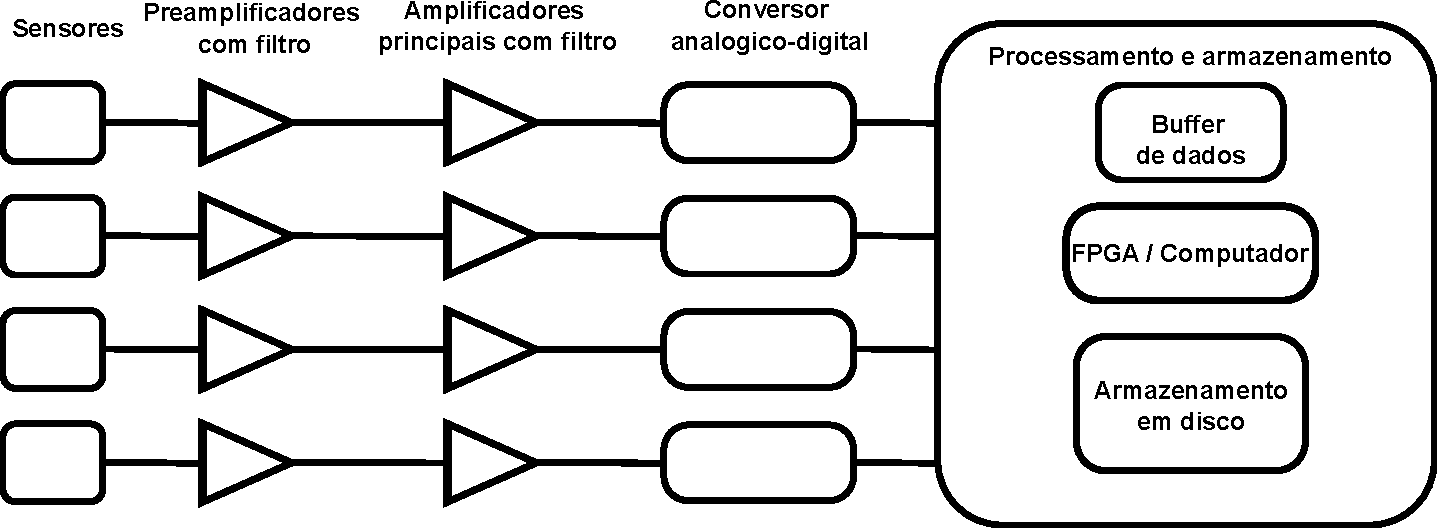
\includegraphics[width=.85\linewidth]{figs/Artigos/nde-ed-org/Figura1.pdf}
    \caption{Esquema funcional de um sistema de EA com sensores piezoelétricos, pré-amplificadores, filtros, amplificadores e aquisição digital. Adaptado de \citeonline{nde-ed-ae-equipment}.}
    \label{fig:nde-ed-org-Fig1}
\end{figure}

Um evento é registrado quando o sinal ultrapassa um \textbf{limiar} (\textit{threshold}) definido acima do ruído. Ele termina quando o sinal permanece abaixo do limiar por um intervalo pré-definido (\textit{hit definition time}, HDT, também chamado de DDT), e segue-se um tempo de bloqueio (\textit{hit lockout time}, HLT) em que novos cruzamentos não iniciam outro evento. Esse procedimento é a \textbf{detecção de \textit{hits}} (\textit{hit detection}), e o evento delimitado é um \textit{hit} \cite{vallen2022,unnthorsson2013}. De cada \textit{hit} extraem-se os parâmetros da Figura~\ref{fig:nde-ed-org-Fig2}: amplitude de pico, tempo de subida, duração, contagens de cruzamentos do limiar e energia. A definição operacional usada neste trabalho é detalhada na Seção~\ref{sec:fund_hits}.

\begin{figure}[htbp]
    \centering
    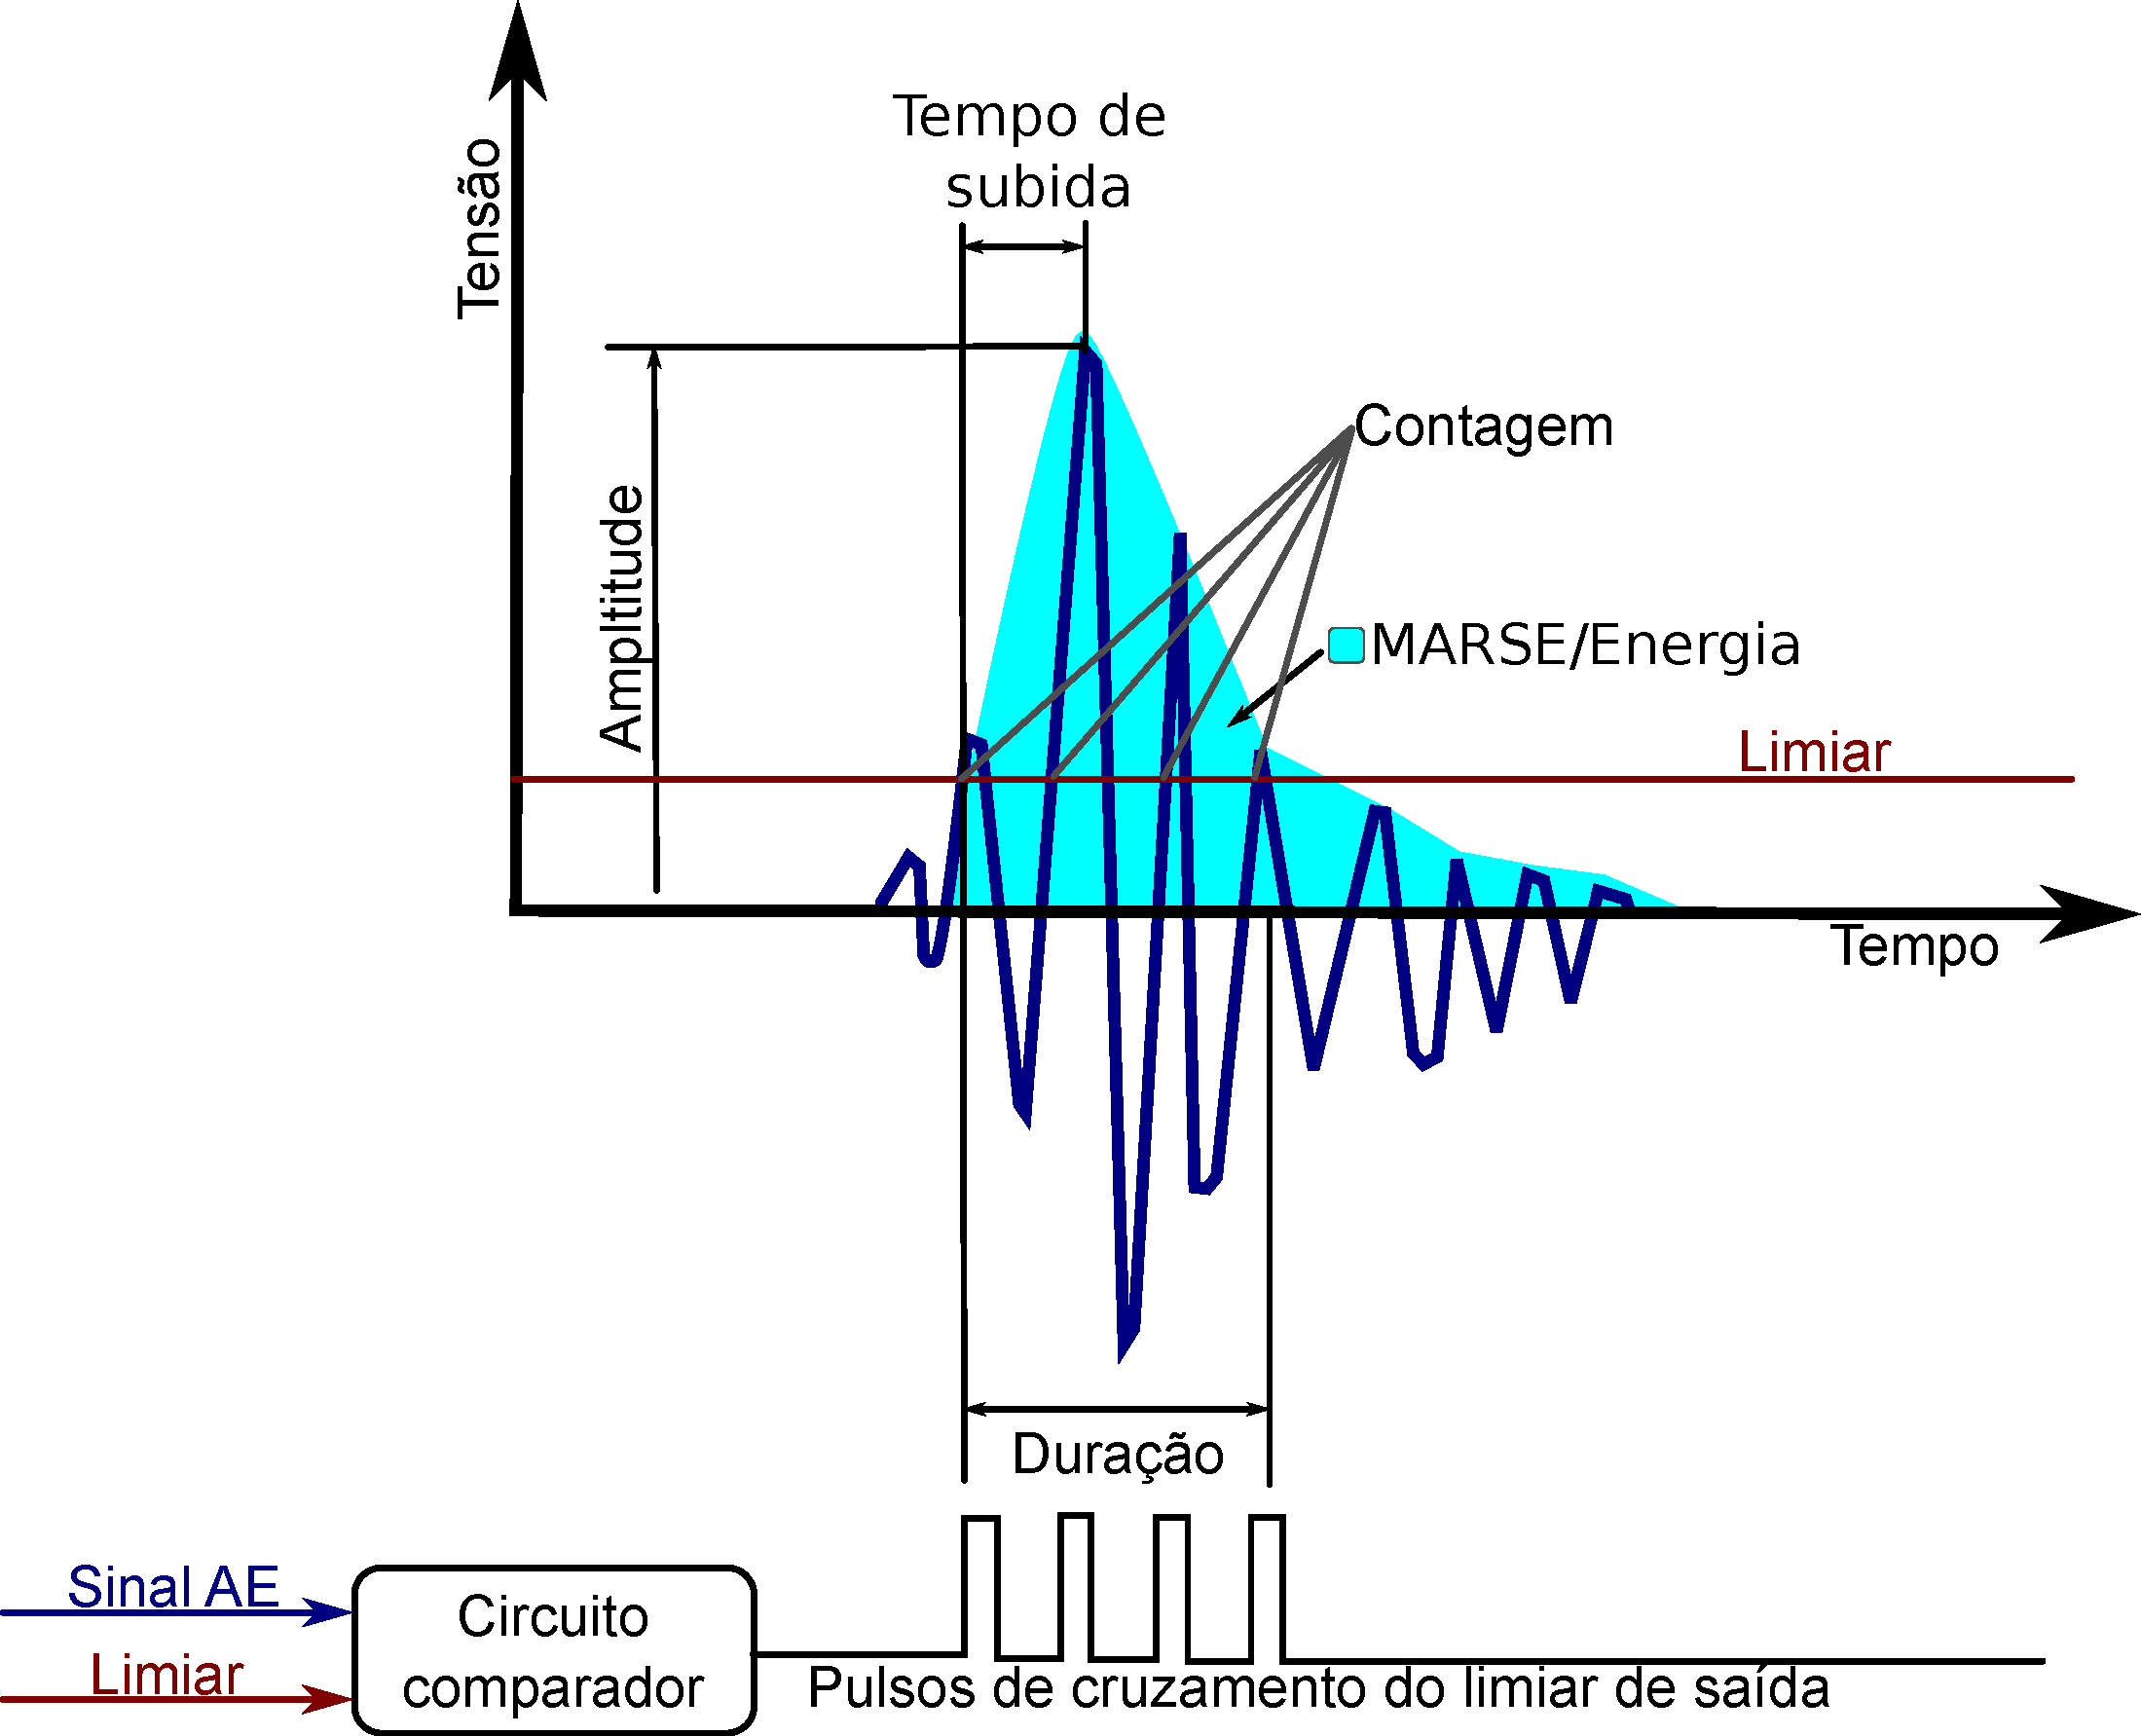
\includegraphics[width=.65\linewidth]{figs/Artigos/nde-ed-org/Figura2.pdf}
    \caption{Parâmetros de um \textit{hit} de EA: amplitude, tempo de subida, duração, contagens e energia (MARSE). Adaptado de \citeonline{nde-ed-ae-equipment}.}
    \label{fig:nde-ed-org-Fig2}
\end{figure}

A energia não tem definição única na literatura. Alguns autores usam a MARSE (\textit{measured area under the rectified signal envelope}, área medida sob o envelope retificado do sinal); outros, a soma dos quadrados do sinal, proporcional à energia elétrica do evento \cite{nde-ed-ae-equipment,liu2023review}. Este trabalho adota a forma quadrática, que é também a do sistema comercial usado como referência (Seção~\ref{sec:fund_hits}). Nem toda EA indica falha: atrito, vazamentos e o próprio escoamento geram sinais semelhantes, chamados de pseudo-fontes, e por isso os parâmetros dos \textit{hits} costumam ser interpretados em conjunto, ao longo do tempo, e não individualmente \cite{grosse2008acoustic}.

\subsection{Detecção de cavitação e trabalhos relacionados}

\citeonline{liu2023review} revisam a detecção de cavitação em bombas por vibração, EA, ruído e pulsação de pressão. Os métodos seguem um fluxo comum (Figura~\ref{fig:LiuFig1}): aquisição, processamento nos domínios do tempo, da frequência ou do tempo-frequência, extração de atributos e reconhecimento do estado por algoritmos de Inteligência Artificial (IA). A EA destaca-se na detecção incipiente, por operar em altas frequências, nas quais os transientes do colapso de bolhas têm relação sinal-ruído elevada \cite{Neill1997Detection,Alfayez2005}.

\begin{figure}[htbp]
    \centering
    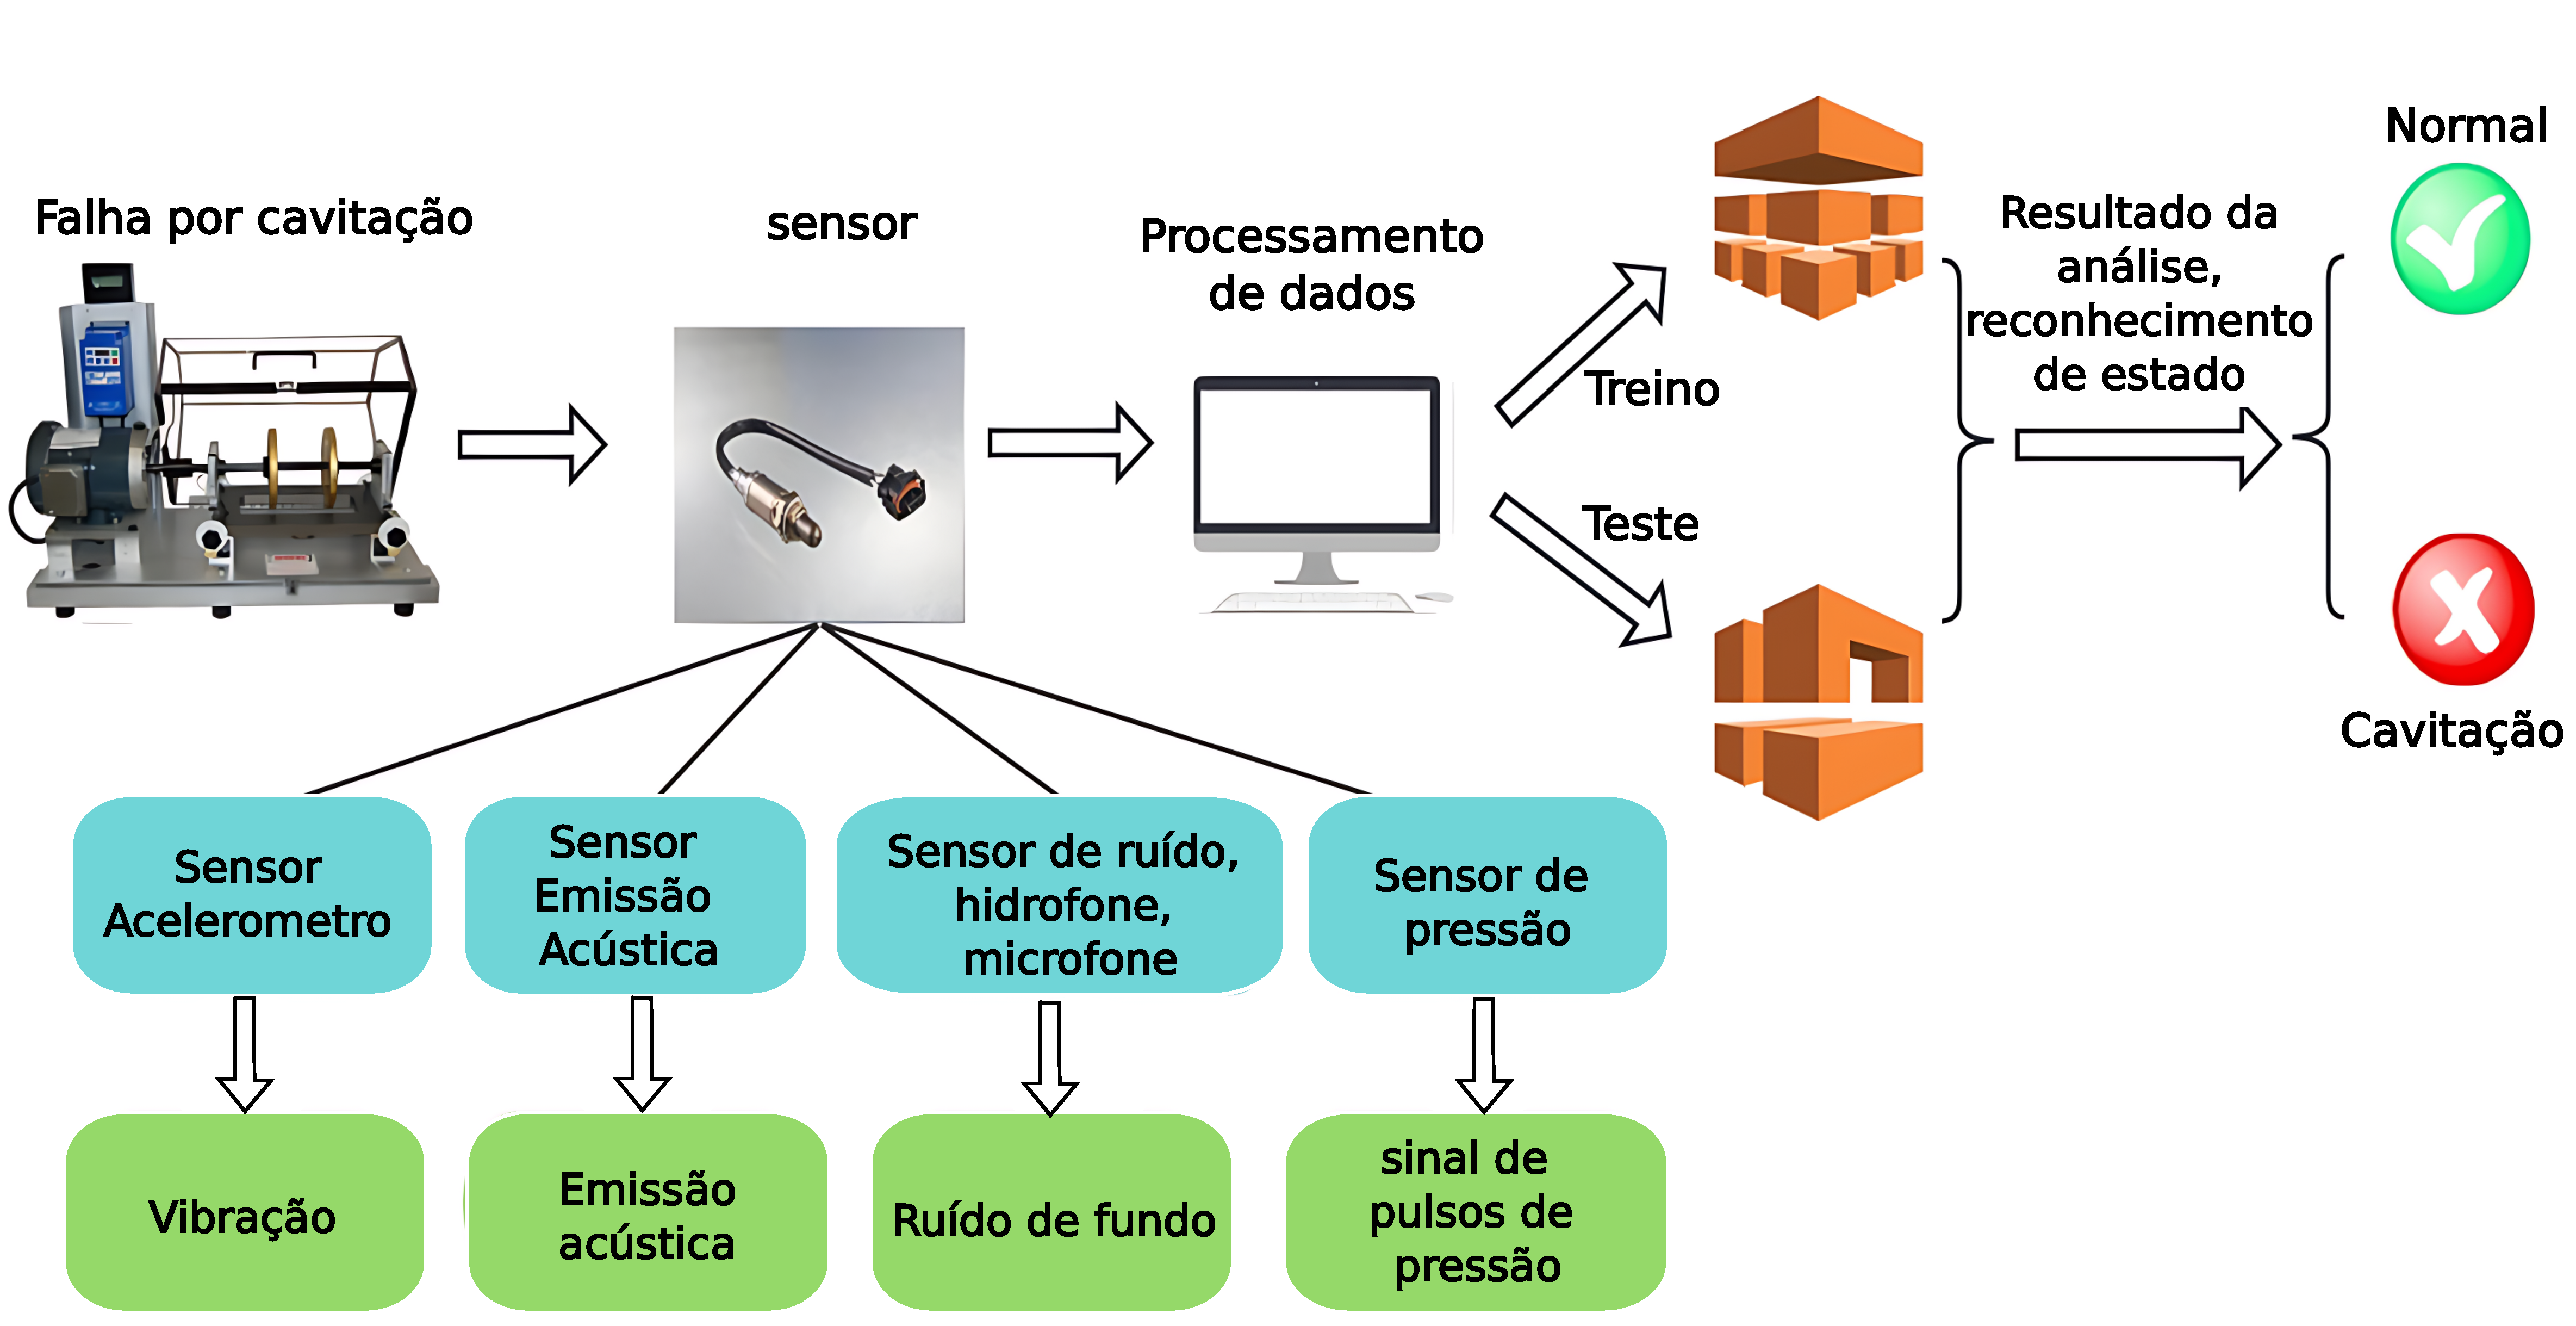
\includegraphics[width=.95\linewidth]{figs/Artigos/Liu/Figura1.pdf}
    \caption{Fluxo básico de detecção de cavitação com base em diferentes sinais. Adaptado de \citeonline{liu2023review}.}
    \label{fig:LiuFig1}
\end{figure}

A Tabela~\ref{tab:sintese_literatura_unificada} resume os trabalhos mais próximos deste, com os resultados relatados. A revisão não aponta um modelo superior de modo absoluto: o desempenho depende do sinal, do delineamento experimental e da validação adotada.

\begin{table}[htbp]
	\footnotesize
	\centering
	\caption{Síntese da literatura: sinais, atributos, modelos e resultados relatados, com destaque para implementações em FPGA.}
	\label{tab:sintese_literatura_unificada}
	\renewcommand{\arraystretch}{1.2}
	\resizebox{\textwidth}{!}{%
		\begin{tabular}{p{2.6cm} p{2.0cm} p{3.6cm} p{3.4cm} p{4.0cm} p{2.6cm}}
			\hline
			\textbf{Alvo} & \textbf{Sinal} & \textbf{Atributos} & \textbf{Modelo / implementação} & \textbf{Resultados relatados} & \textbf{Referências} \\ \hline
			\multicolumn{6}{l}{\textit{Estratégias gerais de detecção de cavitação}} \\ \hline
			Cavitação em bombas & Vibração & RMS, curtose, fator de crista, \textit{cepstrum} & SVM, \textit{Random Forest}, LSTM, CNN & Eficaz em cavitação moderada a severa; menos sensível à incipiente & \citeonline{liu2023review} \\ \hline
			Cavitação em bombas & EA & Amplitude, RMS, energia, contagens & Parâmetros e limiares & Detecção incipiente antes da queda de desempenho & \citeonline{Neill1997Detection,Alfayez2005,Alfayez2005ndt} \\ \hline
			Mancais hidrodinâmicos & EA e vibração & RMS, energia, contagens, tempo-frequência & Comparação e classificação & EA mais sensível nos estágios iniciais & \citeonline{poddar2021classification} \\ \hline
			Cavitação em turbinas & Acústico & Atributos espectrais & \(k\)-NN e GMM & 100\,\% (estático); \(>\)95\,\% (dinâmico) & \citeonline{amini2022development} \\ \hline
			\multicolumn{6}{l}{\textit{Aplicações com implementação em FPGA}} \\ \hline
			Rolamentos & EA & Atributos de EA em taxa ultrassônica & Multinúcleo em FPGA & Diagnóstico em tempo real & \citeonline{kang2015} \\ \hline
			Motores de indução & Corrente & Descritores estatísticos & MLP em FPGA & Precisão de 93,18\,\% & \citeonline{garcia2025detection} \\ \hline
			Qualidade de energia & Tensão & Parâmetros temporais e espectrais & MLP em Artix-7 & Classificação em tempo real & \citeonline{gaona2025fpga} \\ \hline
			Sistemas automotivos & Diversos & Características temporais & MLP em Zynq & Latência \(<\)1\,\(\mu\)s & \citeonline{shreejith2016} \\ \hline
			Rolamentos & Vibração & Envelope e estatísticas & MLP em Zynq-7000 & 95\,\% (tipo) e 89\,\% (severidade), base CWRU & \citeonline{toumi2022fpga} \\ \hline
			\textbf{Este trabalho} & \textbf{EA} & \textbf{Descritores de \textit{hits} por janela} & \textbf{MLP int8 em MicroBlaze ou IP HLS} & \textbf{Ver Capítulo~\ref{chap:resultados}} & --- \\ \hline
	\end{tabular}}
\end{table}

Este trabalho difere dos anteriores em três pontos. A redução de dados é feita na própria lógica, por detecção de \textit{hits} de EA a 10\,MSa/s, e não sobre sinais de baixa taxa. O classificador recebe estatísticas de populações de \textit{hits}, e não atributos de um sinal contínuo, de modo que o fluxo de dados acompanha a atividade acústica, e não a taxa de amostragem. E a avaliação separa as unidades físicas independentes (corridas, sessões ou rolamentos), o que, como se mostra no Capítulo~\ref{chap:resultados}, muda as conclusões em relação às acurácias usualmente relatadas. Os ensaios do MOMEA usam apenas EA; sinais de vibração aparecem só na validação externa com a base CWRU.


\section{Detecção e parametrização de \textit{hits}}
\label{sec:fund_hits}
% Seção 2.2 - Detecção e parametrização de hits (versão enxuta; o título está no Main.tex)

A cadeia de medição determina os descritores tanto quanto a fonte: amplitude, forma de onda e espectro medidos dependem da propagação, do sensor, do acoplamento e da configuração do instrumento. Por isso, comparar instrumentos exige registrar ganho, banda, limiar e parâmetros temporais, referidos ao mesmo ponto da cadeia.

\subsection{Definição operacional do \textit{hit}}
\label{subsec:formalizacao_hit}

Um \textit{hit} é uma unidade de detecção em um único canal, sem correspondência biunívoca com um evento físico: uma fonte pode gerar \textit{hits} em vários sensores, e parâmetros temporais inadequados podem fragmentar uma resposta ou fundir respostas distintas \cite{unnthorsson2013}. Seja \(x[n]\) o código do ADC, amostrado com período \(\Delta t = 1/f_{\mathrm{s}}\). No sistema proposto, o sinal de decisão é a magnitude em relação ao zero calibrado do canal, \(z_{\mathrm{c}}\),
\begin{equation}
	u[n] = \left| x[n] - z_{\mathrm{c}} \right|,
	\label{eq:sinal_decisao}
\end{equation}
e há cruzamento ascendente do limiar \(V_{\mathrm{th}}\) quando \(u[n-1] < V_{\mathrm{th}}\) e \(u[n] \geq V_{\mathrm{th}}\). Sejam \(n_0\) o primeiro cruzamento e \(n_\ell\) o último do mesmo \textit{hit}. O temporizador de definição (DDT, implementado como HDT) é reiniciado a cada amostra acima do limiar, e o \textit{hit} se encerra na \(N_{\mathrm{DDT}}\)-ésima amostra consecutiva de silêncio, com
\begin{equation}
	N_{\mathrm{DDT}} = \left\lceil T_{\mathrm{DDT}} f_{\mathrm{s}} \right\rceil.
	\label{eq:ddt_amostras}
\end{equation}

\subsection{Descritores}
\label{subsec:descritores_hit}
\label{v2:subsec:energia_ea}

Com \(v[n]\) a tensão referida à entrada do pré-amplificador, os descritores são:
\begin{itemize}
	\item \textbf{amplitude de pico}, \(V_{\mathrm{pico}} = \max|v[n]|\), em dB\(_{\mathrm{AE}}\), isto é, \(A = 20\log_{10}(V_{\mathrm{pico}}/1\,\mu\mathrm{V})\);
	\item \textbf{tempo de subida}, do primeiro cruzamento até a primeira ocorrência do pico;
	\item \textbf{duração}, \(t_{\mathrm{dur}} = (n_\ell - n_0)\Delta t\), sem incluir a espera pelo DDT;
	\item \textbf{contagens}, número de cruzamentos ascendentes do limiar no \textit{hit};
	\item \textbf{energia}, na forma quadrática que o AMSY-6 denomina \textit{True Energy} \cite{vallen2022},
	\begin{equation}
		E_{\mathrm{V^2s}} \approx \Delta t\,K_q^2 \sum_{n=n_0}^{n_\ell} u^2[n], \qquad E_{\mathrm{eu}} = \frac{E_{\mathrm{V^2s}}}{10^{-14}\,\mathrm{V^2s}},
		\label{eq:true_energy}
	\end{equation}
	em que \(K_q\) converte um código em volts referidos à entrada; e
	\item \textbf{\textit{Signal Strength}}, \(\Delta t\,K_q\sum|u[n]|\), em nVs.
\end{itemize}
Como \(K_q\) entra ao quadrado, a energia é o descritor mais sensível à calibração. Ela descreve o sinal elétrico, e não a energia mecânica liberada pela fonte.

\subsection{Parâmetros temporais}
\label{subsec:parametros_temporizacao}

As nomenclaturas da literatura e do AMSY-6 não coincidem integralmente \cite{unnthorsson2013,vallen2022}. A Tabela~\ref{tab:parametros_temporizacao} resume a correspondência adotada. O ponto mais delicado é o RAT do AMSY-6, que combina o bloqueio após o \textit{hit} com o agrupamento de \textit{hits} em cascatas; o sistema proposto reproduz o bloqueio e o indicador de rearme, mas não as cascatas. O limiar também interfere na segmentação: valores altos reduzem os \textit{hits} de ruído, mas excluem respostas fracas.

\begin{table}[htbp]
	\centering
	\small
	\caption{Correspondência entre os parâmetros temporais do sistema proposto e do AMSY-6.}
	\label{tab:parametros_temporizacao}
	\begin{tabular}{L{0.20\textwidth}L{0.34\textwidth}L{0.36\textwidth}}
		\toprule
		\textbf{Função} & \textbf{Sistema proposto} & \textbf{AMSY-6} \\
		\midrule
		Encerramento & HDT: expira na \(N_{\mathrm{DDT}}\)-ésima amostra de silêncio & DDT; convenção equivalente \\
		Bloqueio e rearme & HLT re-armável: cruzamento no bloqueio reinicia a espera e marca o \textit{hit} com ROVL & RAT com indicador R; bloqueio equivalente \\
		Cascatas & Não implementadas & Descritores de cascata; não comparáveis \\
		Duração máxima & 100\,ms, indicador MAXDUR & \textit{Timeout} de \(\approx 100\,\mathrm{ms}\) \\
		\bottomrule
	\end{tabular}
\end{table}


% Capítulo 2 - Fundamentação Teórica (versão enxuta): Aprendizado de Máquina e MLP
\section{Aprendizado de Máquina}
\label{sec:AM}

O AM estuda algoritmos que ajustam seus parâmetros a partir de exemplos, em vez de seguir regras programadas manualmente \cite{bishop2006pattern,goodfellow2016deep}. Quanto à forma de aprender, distinguem-se três paradigmas: o supervisionado, em que cada exemplo tem um rótulo conhecido e o modelo aprende a relação entre entradas e saídas; o não supervisionado, que busca estruturas em dados sem rótulo, como agrupamentos ou componentes principais \cite{jolliffe2016}; e o aprendizado por reforço, em que um agente aprende por recompensas ao interagir com um ambiente. Este trabalho trata de classificação supervisionada: cada janela de \textit{hits} recebe o rótulo da condição de operação em que foi registrada.

O objetivo do treinamento não é acertar os exemplos vistos, e sim generalizar para dados novos. A estimativa dessa capacidade depende de como os dados são separados entre treino e teste. Quando as amostras são correlacionadas no tempo ou agrupadas em unidades físicas (corridas, sessões, máquinas), uma partição aleatória coloca amostras quase idênticas nos dois conjuntos e superestima o desempenho; a validação deve então separar grupos inteiros, de modo que o teste contenha apenas unidades não vistas no treino \cite{roberts2017,varma2006}. Esse cuidado orienta os protocolos de validação descritos no Capítulo~\ref{chap:metodos}.

\section{Redes Neurais MLP}
\label{sec:MLP}

Entre os métodos de AM, as RNAs são modelos formados por unidades simples, os neurônios artificiais, que calculam uma soma ponderada das entradas seguida de uma função de ativação \cite{haykin2009neural}. A MLP é uma RNA \textit{feedforward} totalmente conectada, organizada em uma camada de entrada, uma ou mais camadas ocultas e uma camada de saída (Figura~\ref{fig:mlp}); a informação flui da entrada para a saída, sem realimentação \cite{rumelhart1986learning,haykin2009neural}.

\begin{figure}[htbp]
	\centering
	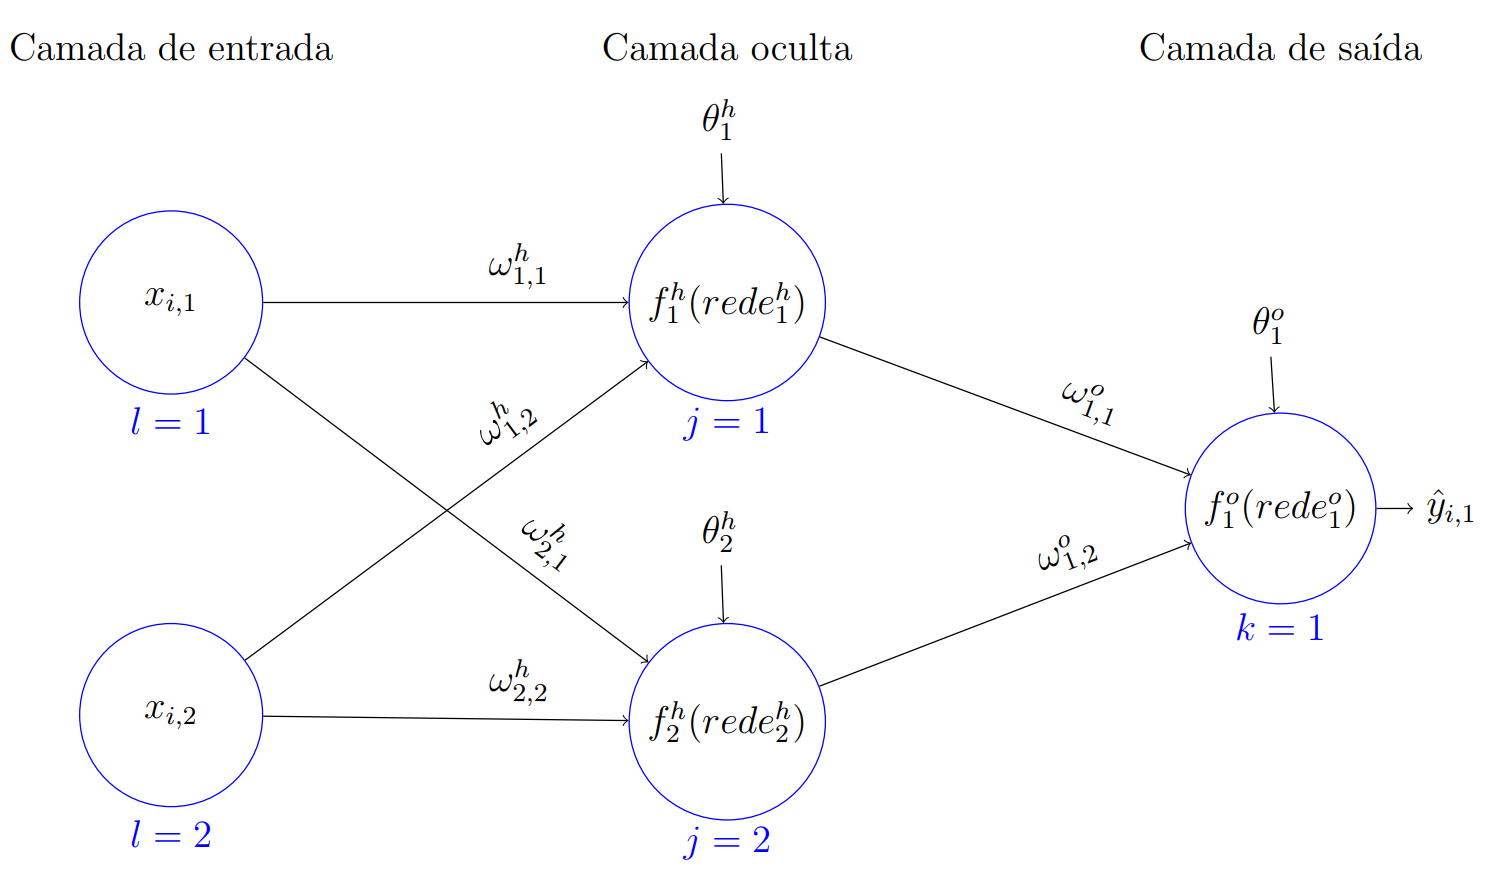
\includegraphics[width=0.8\linewidth]{figs/MLP/MLP}
	\caption{Exemplo de Perceptron Multicamadas. Fonte: o autor.}
	\label{fig:mlp}
\end{figure}

Dado um vetor de entrada \(x \in \mathbb{R}^{d}\), a MLP calcula a saída por transformações afins sucessivas, cada uma seguida de uma não linearidade:
\begin{equation}
	a^{(0)} = x,\qquad
	z^{(\ell)} = W^{(\ell)} a^{(\ell-1)} + b^{(\ell)},\qquad
	a^{(\ell)} = \phi^{(\ell)}\!\big(z^{(\ell)}\big), \quad \ell = 1,\ldots,L,
	\label{eq:mlp_forward}
\end{equation}
em que \(W^{(\ell)}\) e \(b^{(\ell)}\) são os pesos e vieses da camada \(\ell\) e \(\phi^{(\ell)}\) é a função de ativação. Nas camadas ocultas usa-se em geral a ReLU, \(\phi(z)=\max(0,z)\), que é barata de calcular e se reduz a uma comparação em \textit{hardware}. Na classificação, a camada de saída tem um neurônio por classe e a função \textit{softmax} converte os escores em probabilidades; a classe prevista é a de maior escore. É a não linearidade das camadas ocultas que permite separar classes não linearmente separáveis: uma MLP com uma única camada oculta e neurônios suficientes aproxima qualquer função contínua com precisão arbitrária \cite{cybenko1989approximation,hornik1991approximation}.

O treinamento ajusta os parâmetros \(\theta=\{(W^{(\ell)},b^{(\ell)})\}_{\ell=1}^{L}\) minimizando a perda empírica com regularização,
\begin{equation}
	\min_{\theta}\;\; \frac{1}{N}\sum_{i=1}^{N}\mathcal{L}\big(f_{\theta}(x_i),y_i\big)\;+\;\lambda\,\Omega(\theta),
	\label{eq:mlp_perda}
\end{equation}
em que \(\mathcal{L}\) é a entropia cruzada e \(\Omega(\theta)\), em geral, a norma \(\ell_2\) dos pesos. O gradiente é obtido por retropropagação (\textit{backpropagation}), que aplica a regra da cadeia às camadas da rede \cite{rumelhart1986learning}, e os parâmetros são atualizados por gradiente descendente estocástico em mini-lotes (Algoritmo~\ref{alg:mlp_sgd_minibatch}) ou por variantes adaptativas, como o Adam \cite{kingma2015adam}. A parada antecipada, que interrompe o treinamento quando o erro em um conjunto de validação deixa de cair, é outra forma usual de limitar o sobreajuste \cite{prechelt1998}.

\begin{algorithm}[htbp]
	\caption{Treinamento de uma MLP por gradiente descendente estocástico em mini-lotes}
	\label{alg:mlp_sgd_minibatch}
	\begin{algorithmic}[1]
		\Require Treino \(\mathcal{D}=\{(x_i,y_i)\}_{i=1}^{N}\); taxa \(\eta>0\); mini-lote \(B\); épocas \(E\)
		\Ensure Parâmetros treinados \(\theta\)
		\State Inicializar \(\theta\) aleatoriamente (Xavier ou He)
		\For{\(e = 1,\dots,E\)}
		\State Embaralhar \(\mathcal{D}\)
		\For{cada mini-lote \(\mathcal{B}\subset\mathcal{D}\), \(|\mathcal{B}|=B\)}
		\State Propagar \(\hat{y}=f_{\theta}(x)\) e calcular a perda \(J_{\mathcal{B}}(\theta)\)
		\State Retropropagar: \(g \gets \nabla_{\theta} J_{\mathcal{B}}(\theta)\)
		\State Atualizar: \(\theta \gets \theta - \eta g\)
		\EndFor
		\EndFor
		\State \Return \(\theta\)
	\end{algorithmic}
\end{algorithm}

Modelos mais complexos, como as redes convolucionais, superam as MLPs quando a entrada tem estrutura espacial ou sequencial explícita, mas, sobre atributos já extraídos, a MLP continua competitiva \cite{abd2023multi}. Sua inferência se reduz a produtos matriz-vetor e funções simples, com número de operações conhecido de antemão, o que favorece o mapeamento em FPGA, discutido a seguir \cite{Shawahna2019}.


% Capítulo 2 - Fundamentação Teórica (versão enxuta): FPGAs e MLP em FPGA
\section{\textit{Field-Programmable Gate Arrays} (FPGAs)}
\label{sec:FPGA}

Os FPGAs são circuitos integrados cuja lógica interna é configurada após a fabricação. Diferem dos circuitos integrados de aplicação específica (\textit{Application-Specific Integrated Circuits}, ASICs), que executam uma função fixa, e dos processadores, que executam instruções em sequência: no FPGA, o algoritmo é descrito em uma linguagem de descrição de \textit{hardware} (\textit{Hardware Description Language}, HDL), como VHDL ou Verilog, e convertido em um circuito digital dedicado, com operações paralelas e latência determinística \cite{kuon2008fpga,trimberger2015three}. Essa combinação de reconfigurabilidade, paralelismo e baixa latência faz do FPGA uma plataforma adequada à aquisição e ao processamento de sinais em alta taxa e à inferência de redes neurais embarcadas \cite{Shawahna2019}.

\subsection{Arquitetura e recursos}

Um FPGA é uma matriz de blocos lógicos ligados por uma rede de interconexão programável e complementados por blocos dedicados (Figura~\ref{fig:FPGA_internal_architeture}) \cite{langhammer2014design}. Os recursos que limitam um projeto, e que são relatados neste trabalho, são:
\begin{itemize}
	\item \textbf{LUTs e \textit{flip-flops}}: os blocos lógicos configuráveis (\textit{Configurable Logic Blocks}, CLBs) contêm tabelas de consulta (\textit{Look-Up Tables}, LUTs), que implementam funções lógicas arbitrárias de poucas entradas, e \textit{flip-flops}, que armazenam estado;
	\item \textbf{BRAM}: blocos de memória interna, usados como \textit{buffers} e para guardar coeficientes e dados intermediários sem acesso à memória externa;
	\item \textbf{DSP}: blocos aritméticos dedicados a multiplicação e acumulação (\textit{multiply-accumulate}, MAC), a operação básica de filtros e camadas densas;
	\item \textbf{blocos de entrada e saída}, que fazem a interface com conversores, memórias e redes de comunicação.
\end{itemize}

\begin{figure}[htbp]
    \centering
    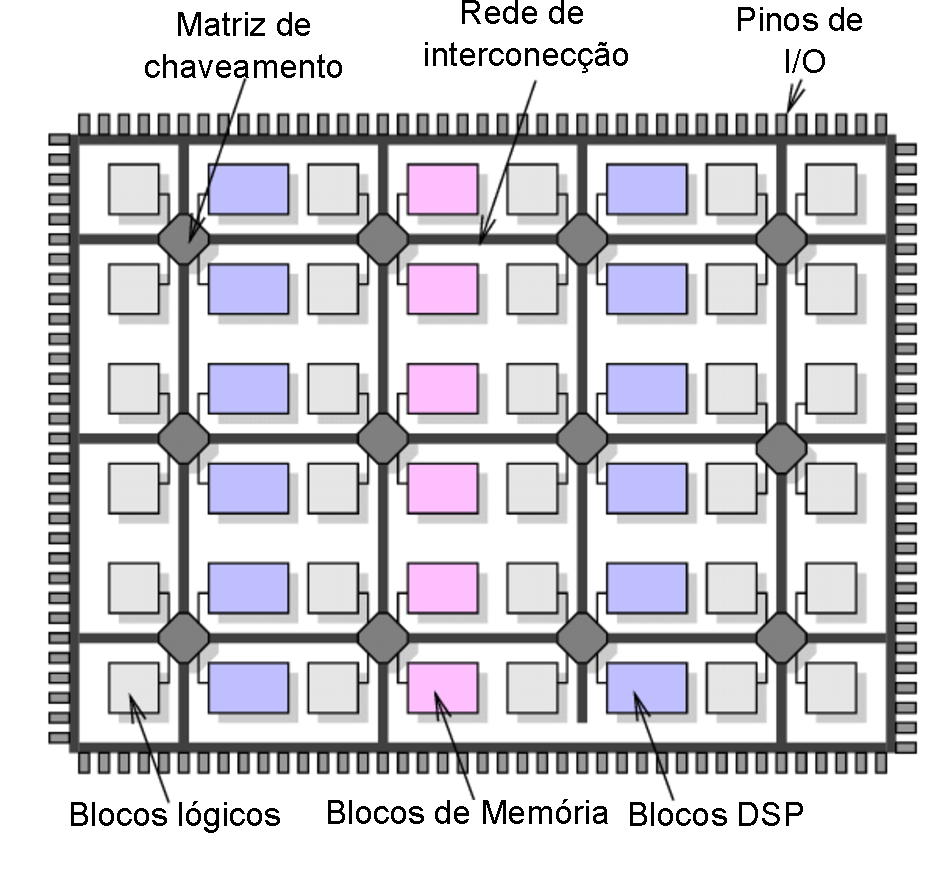
\includegraphics[width=0.6\linewidth]{figs/FPGA/FPGA.pdf}
    \caption{Arquitetura interna de um FPGA. Adaptado de \citeonline{langhammer2014design}.}
    \label{fig:FPGA_internal_architeture}
\end{figure}

Parte da lógica pode ser usada para instanciar um processador \textit{soft-core}, como o MicroBlaze da AMD, que executa código C sobre a lógica programável e se comunica com os demais blocos por barramentos AXI \cite{amd_ug984}. O projeto pode então ser particionado: funções de controle, comunicação e cálculo pouco crítico ficam em \textit{software}, enquanto as operações intensivas ou de latência estrita são implementadas em lógica dedicada.

\subsection{Fluxo de desenvolvimento}

A Figura~\ref{fig:FluxoDesenvolvimentoFPGA} resume o fluxo de desenvolvimento. Parte-se do algoritmo ou do modelo, que é otimizado (por exemplo, quantizado) e descrito em HDL ou em C/C++ para síntese de alto nível (\textit{High-Level Synthesis}, HLS). Na HLS, a ferramenta converte o código C em um circuito, e o projetista orienta o paralelismo por diretivas, como \textit{pipeline} e desenrolamento de laços \cite{cong2011hls,amd_ug1399}. Seguem a síntese lógica, que mapeia o projeto em LUTs, \textit{flip-flops}, DSPs e BRAMs, o posicionamento e roteamento (\textit{place \& route}) e a análise estática de temporização, que verifica se todos os caminhos cumprem o período de \textit{clock}. O fluxo é iterativo: os relatórios de recursos e de temporização e a verificação por simulação e em \textit{hardware} realimentam as etapas anteriores \cite{amd_ug900}.

\begin{figure}[htbp]
    \centering
    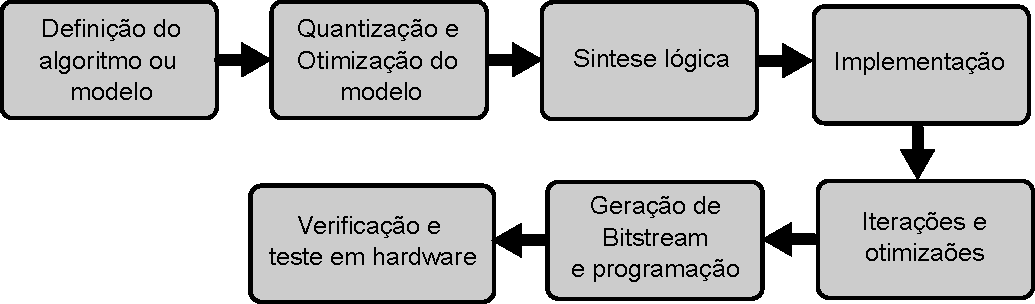
\includegraphics[width=0.75\linewidth]{figs/FPGA/FluxoOtimização.pdf}
    \caption{Fluxo de desenvolvimento e otimização de projetos em FPGA. Fonte: o autor.}
    \label{fig:FluxoDesenvolvimentoFPGA}
\end{figure}

\subsection{Quantização}

A técnica de otimização mais usada para executar redes neurais em FPGAs é a quantização: pesos e ativações deixam de ser representados em ponto flutuante de 32 bits e passam a inteiros de 8 bits ou menos, o que reduz memória, DSPs e lógica, com perda de acurácia em geral pequena \cite{jacob2018,nagel2021}. Na quantização afim, um valor real \(r\) é representado por um inteiro \(q\) com escala \(s\) e ponto zero \(z\),
\begin{equation}
	r \approx s\,(q - z), \qquad q = \mathrm{clip}\!\left(\mathrm{round}(r/s) + z,\; q_{\min},\; q_{\max}\right),
	\label{eq:quantizacao}
\end{equation}
e, na forma simétrica (\(z=0\)), comum para os pesos, \(s = \max|r|/127\) em int8. Os produtos de uma camada densa são acumulados em 32 bits e reescalados para a camada seguinte, de modo que toda a inferência usa só aritmética inteira. A quantização pode ser aplicada após o treinamento ou simulada durante ele (\textit{quantization-aware training}). Outras técnicas, como poda de conexões, fusão de camadas, \textit{pipeline} e uso de memória local, complementam a quantização \cite{Shawahna2019,mouri2025optimizing}.

\subsection{MLP em FPGA para diagnóstico de falhas}
\label{subsection:MLP}

Há diversas implementações de MLPs em FPGA. Alguns trabalhos tratam do custo da implementação: estimativa de recursos antes da síntese \cite{kokkinis2025fast}, poda e quantização \cite{ron2022experimental}, funções de ativação adequadas ao \textit{hardware} \cite{si2020neural}, co-projeto automático da rede e do circuito \cite{colangelo2020automl} e arquiteturas em \textit{pipeline} \cite{bahoura2011fpga}. No diagnóstico de máquinas, \citeonline{garcia2025detection} classificam curtos-circuitos incipientes entre espiras de motores de indução com uma MLP alimentada por descritores estatísticos da corrente, com precisão de 93,18\,\%. \citeonline{gaona2025fpga} classificam distúrbios de qualidade de energia com uma MLP 3-6-6 em um Artix-7. \citeonline{shreejith2016} usam reconfiguração parcial em um Zynq para alternar entre uma rede de detecção e outra que substitui um sensor defeituoso, com latência abaixo de 1\,\(\mu\)s. Por fim, \citeonline{toumi2022fpga} extraem atributos de envelope da vibração e os classificam com uma MLP em ponto fixo em um Zynq-7000, atingindo 95\,\% de acurácia no tipo de falha e 89\,\% na severidade na base CWRU, com coerência entre simulação e \textit{hardware}.

Esses trabalhos partem de sinais de baixa taxa (corrente, tensão, vibração), e nenhum combina detecção de \textit{hits} de EA na lógica com uma MLP sobre os descritores resultantes, que é a proposta deste trabalho.


\chapter{Materiais e Métodos}
\label{chap:metodos}
% =======================================================================================================
% Capítulo 3 - Materiais e Métodos
% As seções 3.3 a 3.8 incorporam, revisados, os relatórios do projeto (ver capitulos/importado/).
% =======================================================================================================

Este capítulo descreve o sistema desenvolvido e os procedimentos usados para avaliá-lo. A Seção~\ref{sec:mm_visao} apresenta a visão geral da proposta e delimita o que já existia no Projeto MOMEA e o que constitui contribuição desta dissertação. A Seção~\ref{sec:mm_antecedentes} resume a plataforma de aquisição contínua que antecedeu este trabalho. As Seções~\ref{sec:mm_decisoes} a~\ref{sec:mm_delineamento} tratam do extrator de \textit{hits} em FPGA: as decisões de projeto, a implementação e o delineamento do ensaio comparativo com um sistema comercial. As Seções~\ref{sec:mm_bomba} a~\ref{sec:mm_cwru} descrevem o uso dos registros de \textit{hits} para classificar condições de operação, a implementação embarcada dessa classificação e a validação externa em uma base pública. A Seção~\ref{sec:mm_ferramentas} lista as ferramentas utilizadas.

% -------------------------------------------------------------------------------------------------------
\section{Visão geral da proposta}
\label{sec:mm_visao}

A Figura~\ref{fig:pipeline_proposto} resume a cadeia proposta. O sinal de EA é captado por um sensor piezoelétrico, amplificado e digitalizado a 10\,MSa/s. Em vez de transmitir todas as amostras, a lógica programável do FPGA detecta os \textit{hits} e calcula seus descritores (amplitude, contagens, tempo de subida, duração e energia), de modo que cada \textit{hit} é reduzido a um registro de 32 bytes. Esses registros são então agregados em janelas de tempo, das quais se extraem descritores estatísticos que alimentam uma rede MLP. A classificação pode ocorrer no computador, como nos ensaios com a bomba, ou no próprio FPGA, no processador embarcado MicroBlaze ou em um acelerador gerado por síntese de alto nível (HLS).

\begin{figure}[htbp]
	\centering
	\resizebox{\textwidth}{!}{%
	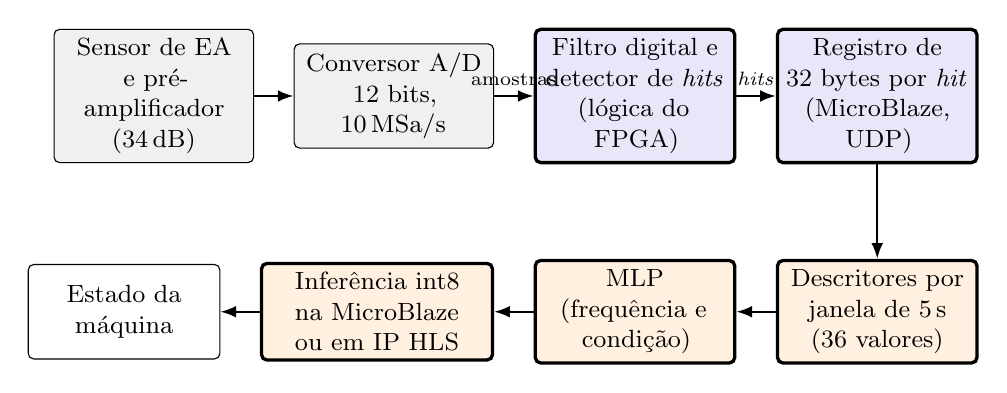
\begin{tikzpicture}[
		font=\small, node distance=5mm and 5mm,
		bloco/.style={draw, rounded corners=2pt, align=center, minimum height=12mm, text width=23mm},
		exist/.style={bloco, fill=gray!12},
		novo/.style={bloco, fill=blue!10, very thick},
		sw/.style={bloco, fill=orange!12, very thick},
		seta/.style={-{Latex[length=2mm]}, thick}]
		\node[exist] (sens) {Sensor de EA\\e pré-amplificador\\(34\,dB)};
		\node[exist, right=of sens] (adc) {Conversor A/D\\12 bits,\\10\,MSa/s};
		\node[novo, right=of adc] (hit) {Filtro digital e\\detector de \textit{hits}\\(lógica do FPGA)};
		\node[novo, right=of hit] (reg) {Registro de\\32 bytes por \textit{hit}\\(MicroBlaze, UDP)};
		\node[sw, below=12mm of reg] (jan) {Descritores por\\janela de 5\,s\\(36 valores)};
		\node[sw, left=of jan] (mlp) {MLP\\(frequência e\\condição)};
		\node[sw, left=of mlp, text width=27mm] (emb) {Inferência int8\\na MicroBlaze\\ou em IP HLS};
		\node[bloco, left=of emb, text width=22mm] (dec) {Estado da\\máquina};
		\draw[seta] (sens) -- (adc);
		\draw[seta] (adc) -- node[above, font=\scriptsize]{amostras} (hit);
		\draw[seta] (hit) -- node[above, font=\scriptsize]{\textit{hits}} (reg);
		\draw[seta] (reg) -- (jan);
		\draw[seta] (jan) -- (mlp);
		\draw[seta] (mlp) -- (emb);
		\draw[seta] (emb) -- (dec);
	\end{tikzpicture}}
	\caption[Cadeia proposta: extração de \textit{hits} na borda e classificação por MLP]{Cadeia proposta. Em cinza, elementos que já existiam no Projeto MOMEA; em azul, o extrator de \textit{hits} em FPGA desenvolvido neste trabalho (Seções~\ref{sec:mm_decisoes} a~\ref{sec:mm_delineamento}); em laranja, a classificação a partir dos registros e sua implementação embarcada (Seções~\ref{sec:mm_bomba} a~\ref{sec:mm_cwru}). Fonte: o autor.}
	\label{fig:pipeline_proposto}
\end{figure}

Essa organização responde a uma questão central do trabalho: por que usar aprendizado de máquina se a detecção já seleciona os trechos que ultrapassam o limiar? As duas etapas têm papéis distintos. A detecção de \textit{hits} é uma etapa de \emph{redução de dados e extração de atributos}: ela descarta o ruído de fundo e resume cada evento em poucos números, mas não interpreta o que os eventos significam. Um único \textit{hit} não indica, por si só, a condição da máquina, porque eventos de mesma amplitude podem vir de cavitação, de impactos mecânicos ou de ruído hidráulico. A condição se manifesta na \emph{população} de \textit{hits} ao longo do tempo (taxa, distribuição de amplitudes e energias, duração, periodicidade), e é essa população que o classificador interpreta. Assim, o limiar decide \emph{o que} é registrado; o modelo decide \emph{o que} os registros indicam.

\subsection{Delimitação das contribuições}

Para deixar claro o que é contribuição desta dissertação, distinguem-se três grupos de elementos:
\begin{itemize}
	\item \textbf{pré-existentes no Projeto MOMEA}: sensores, pré-amplificadores e bancada; a plataforma de aquisição contínua MomeaProbe/MomeaCapture, com interface USB~3.0 (Seção~\ref{sec:mm_antecedentes}); e os estudos com redes convolucionais sobre espectrogramas, conduzidos por outro membro da equipe;
	\item \textbf{desenvolvidos nesta dissertação}: o extrator de \textit{hits} em FPGA, com registro compacto e comunicação por UDP (Seções~\ref{sec:mm_decisoes} e~\ref{sec:mm_implementacao}); sua avaliação em ensaio simultâneo com o sistema comercial Vallen AMSY-6 (Seção~\ref{sec:mm_delineamento}); a classificação das condições de operação de uma bomba a partir dos registros de \textit{hits} (Seção~\ref{sec:mm_bomba}); a implementação da classificação em int8, na MicroBlaze e em lógica dedicada, verificada por simulação (Seção~\ref{sec:mm_embarcado}); e a validação externa do método em uma base pública de rolamentos (Seção~\ref{sec:mm_cwru});
	\item \textbf{realizados apenas em simulação}: a execução da inferência na placa. O processador MicroBlaze e o acelerador HLS foram verificados por simulação RTL e por síntese, mas não executados no \textit{hardware}, pelos motivos discutidos na Seção~\ref{sec:mm_embarcado}.
\end{itemize}

\subsection{Bases de dados utilizadas}

A Tabela~\ref{tab:bases} resume as bases usadas, seu tamanho e a forma como foram divididas entre treino e teste. A base de bombas do UWA \textit{System Health Lab}, prevista na qualificação, não foi utilizada: os registros de \textit{hits} do próprio MOMEA e a base CWRU cobriram, respectivamente, a aplicação-alvo e a necessidade de uma referência pública.

\begin{table}[htbp]
	\centering
	\small
	\caption{Bases de dados utilizadas, tamanho e divisão entre treino e teste.}
	\label{tab:bases}
	\setlength{\tabcolsep}{4pt}
	\begin{tabular}{L{0.17\textwidth}L{0.29\textwidth}L{0.19\textwidth}L{0.24\textwidth}}
		\toprule
		\textbf{Base} & \textbf{Conteúdo} & \textbf{Tamanho} & \textbf{Divisão treino/teste} \\
		\midrule
		Ensaio elétrico R1 & \textit{Bursts} senoidais injetados simultaneamente no MOMEA e no AMSY-6 & 48\,303 estímulos; 3 frequências e 5 taxas & Não há treino: comparação de instrumentos \\
		Bancada da bomba (MOMEA) & Registros de \textit{hits} de 2 canais em 56 corridas (8 frequências \(\times\) 7 configurações de válvulas) & 283\,618 \textit{hits}; 3\,540 janelas de 5\,s; 36 descritores & Validação cruzada sem sorteio de \textit{hits}: blocos de tempo, corrida e série deixadas de fora \\
		CWRU (48\,kHz, lado do acionamento) & Vibração com rolamento são e com defeitos na pista interna, na esfera e na pista externa & 40 gravações; 1\,376 janelas de 0,25\,s & Janelas sorteadas, carga e diâmetro do defeito deixados de fora \\
		\bottomrule
	\end{tabular}
\end{table}

Em nenhuma das validações \textit{hits} ou janelas de uma mesma gravação foram sorteados livremente entre treino e teste como critério principal, porque isso superestima o desempenho, como se mostra nos Capítulos~\ref{chap:resultados} e na literatura \cite{kaufman2012,roberts2017}. O sorteio aparece apenas como referência, para tornar visível o tamanho desse viés.

% -------------------------------------------------------------------------------------------------------
\section{Antecedentes: aquisição contínua no Projeto MOMEA}
\label{sec:mm_antecedentes}

Na etapa inicial do Projeto MOMEA, foi desenvolvida a plataforma \textbf{MomeaProbe/MomeaCapture}. O MomeaProbe é o \textit{hardware} de aquisição, com dois conversores A/D de 12 bits a 8\,MSa/s e transmissão por USB~3.0 (Figura~\ref{fig:MomeaProbe12USB}). O MomeaCapture é a aplicação em C++/Qt que recebe, compacta, armazena em banco de dados e exibe os sinais (Figura~\ref{fig:MomeaCapture}). Essa infraestrutura permitiu registrar longas séries temporais contínuas, a partir das quais outro membro da equipe treinou redes convolucionais bidimensionais sobre espectrogramas para classificar regimes de cavitação.

\begin{figure}[htbp]
	\centering
	\begin{subfigure}[b]{0.38\textwidth}
		\centering
		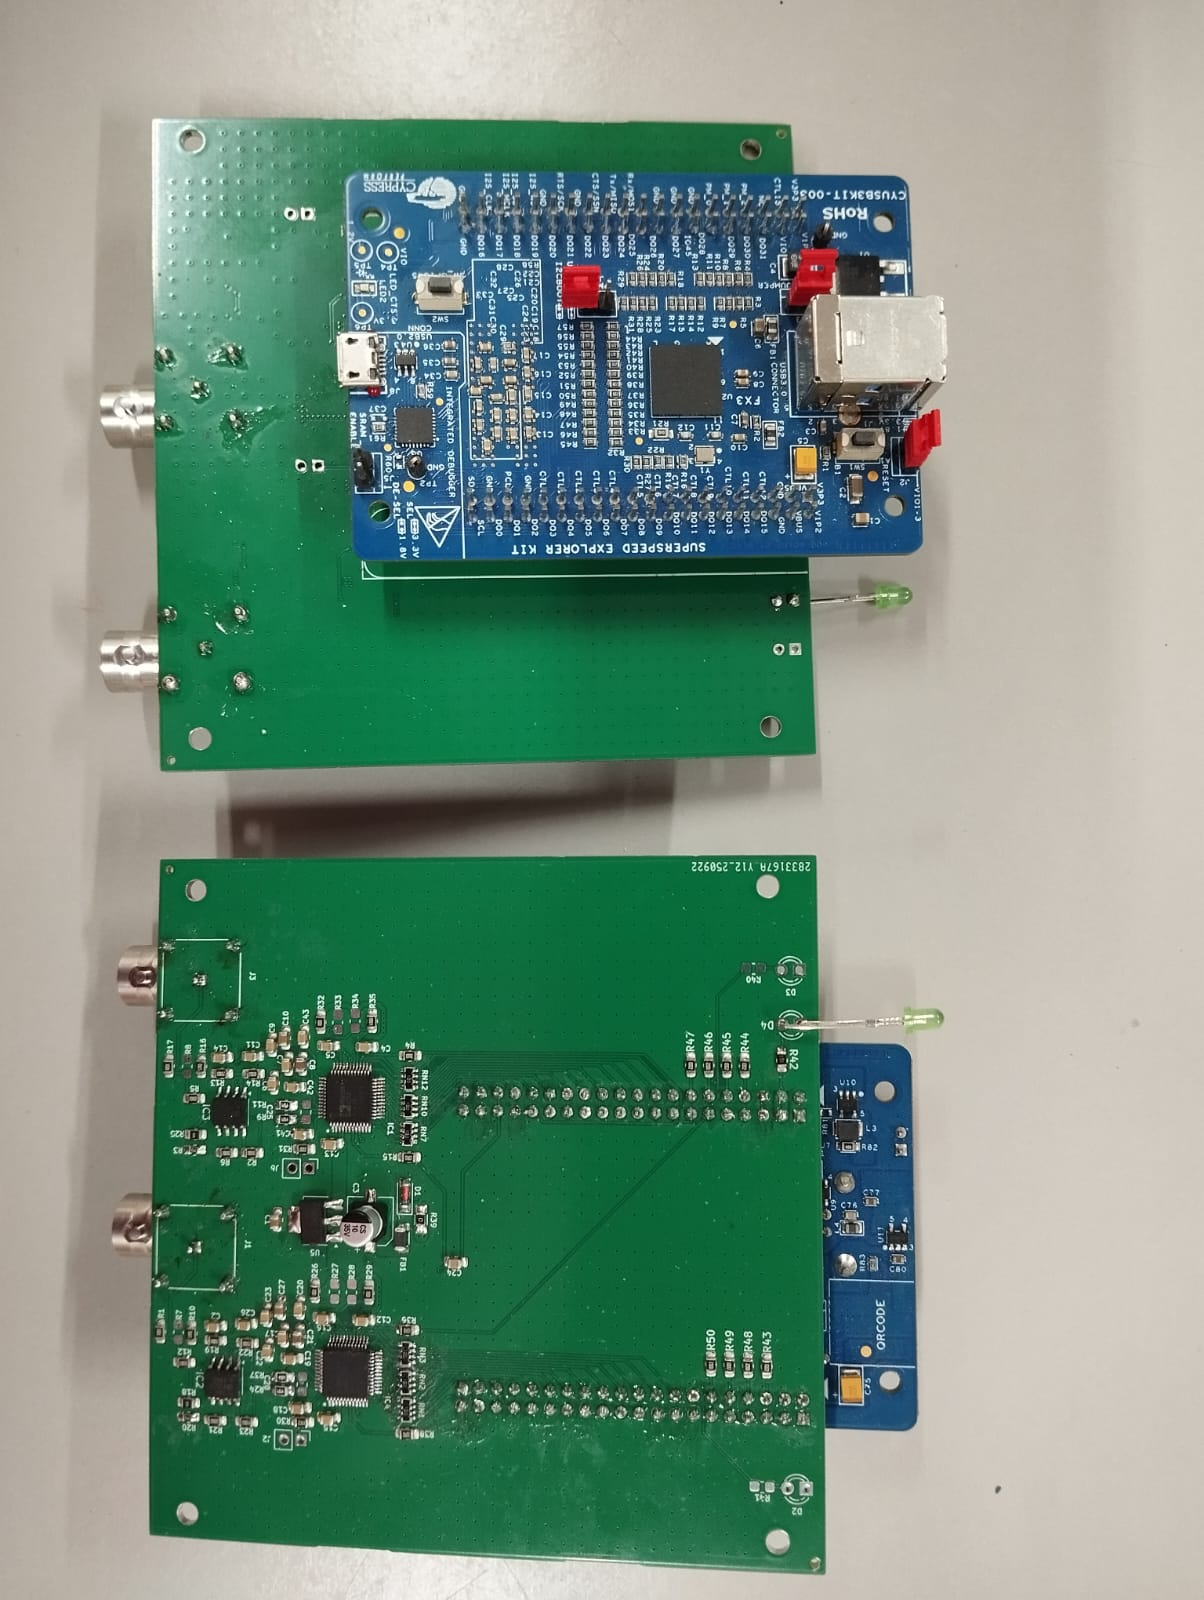
\includegraphics[angle=90, width=\linewidth]{figs/PlacasADC_AD9226.jpeg}
		\caption{Placas de captura MomeaProbe12USB.}
		\label{fig:MomeaProbe12USB}
	\end{subfigure}\hfill
	\begin{subfigure}[b]{0.58\textwidth}
		\centering
		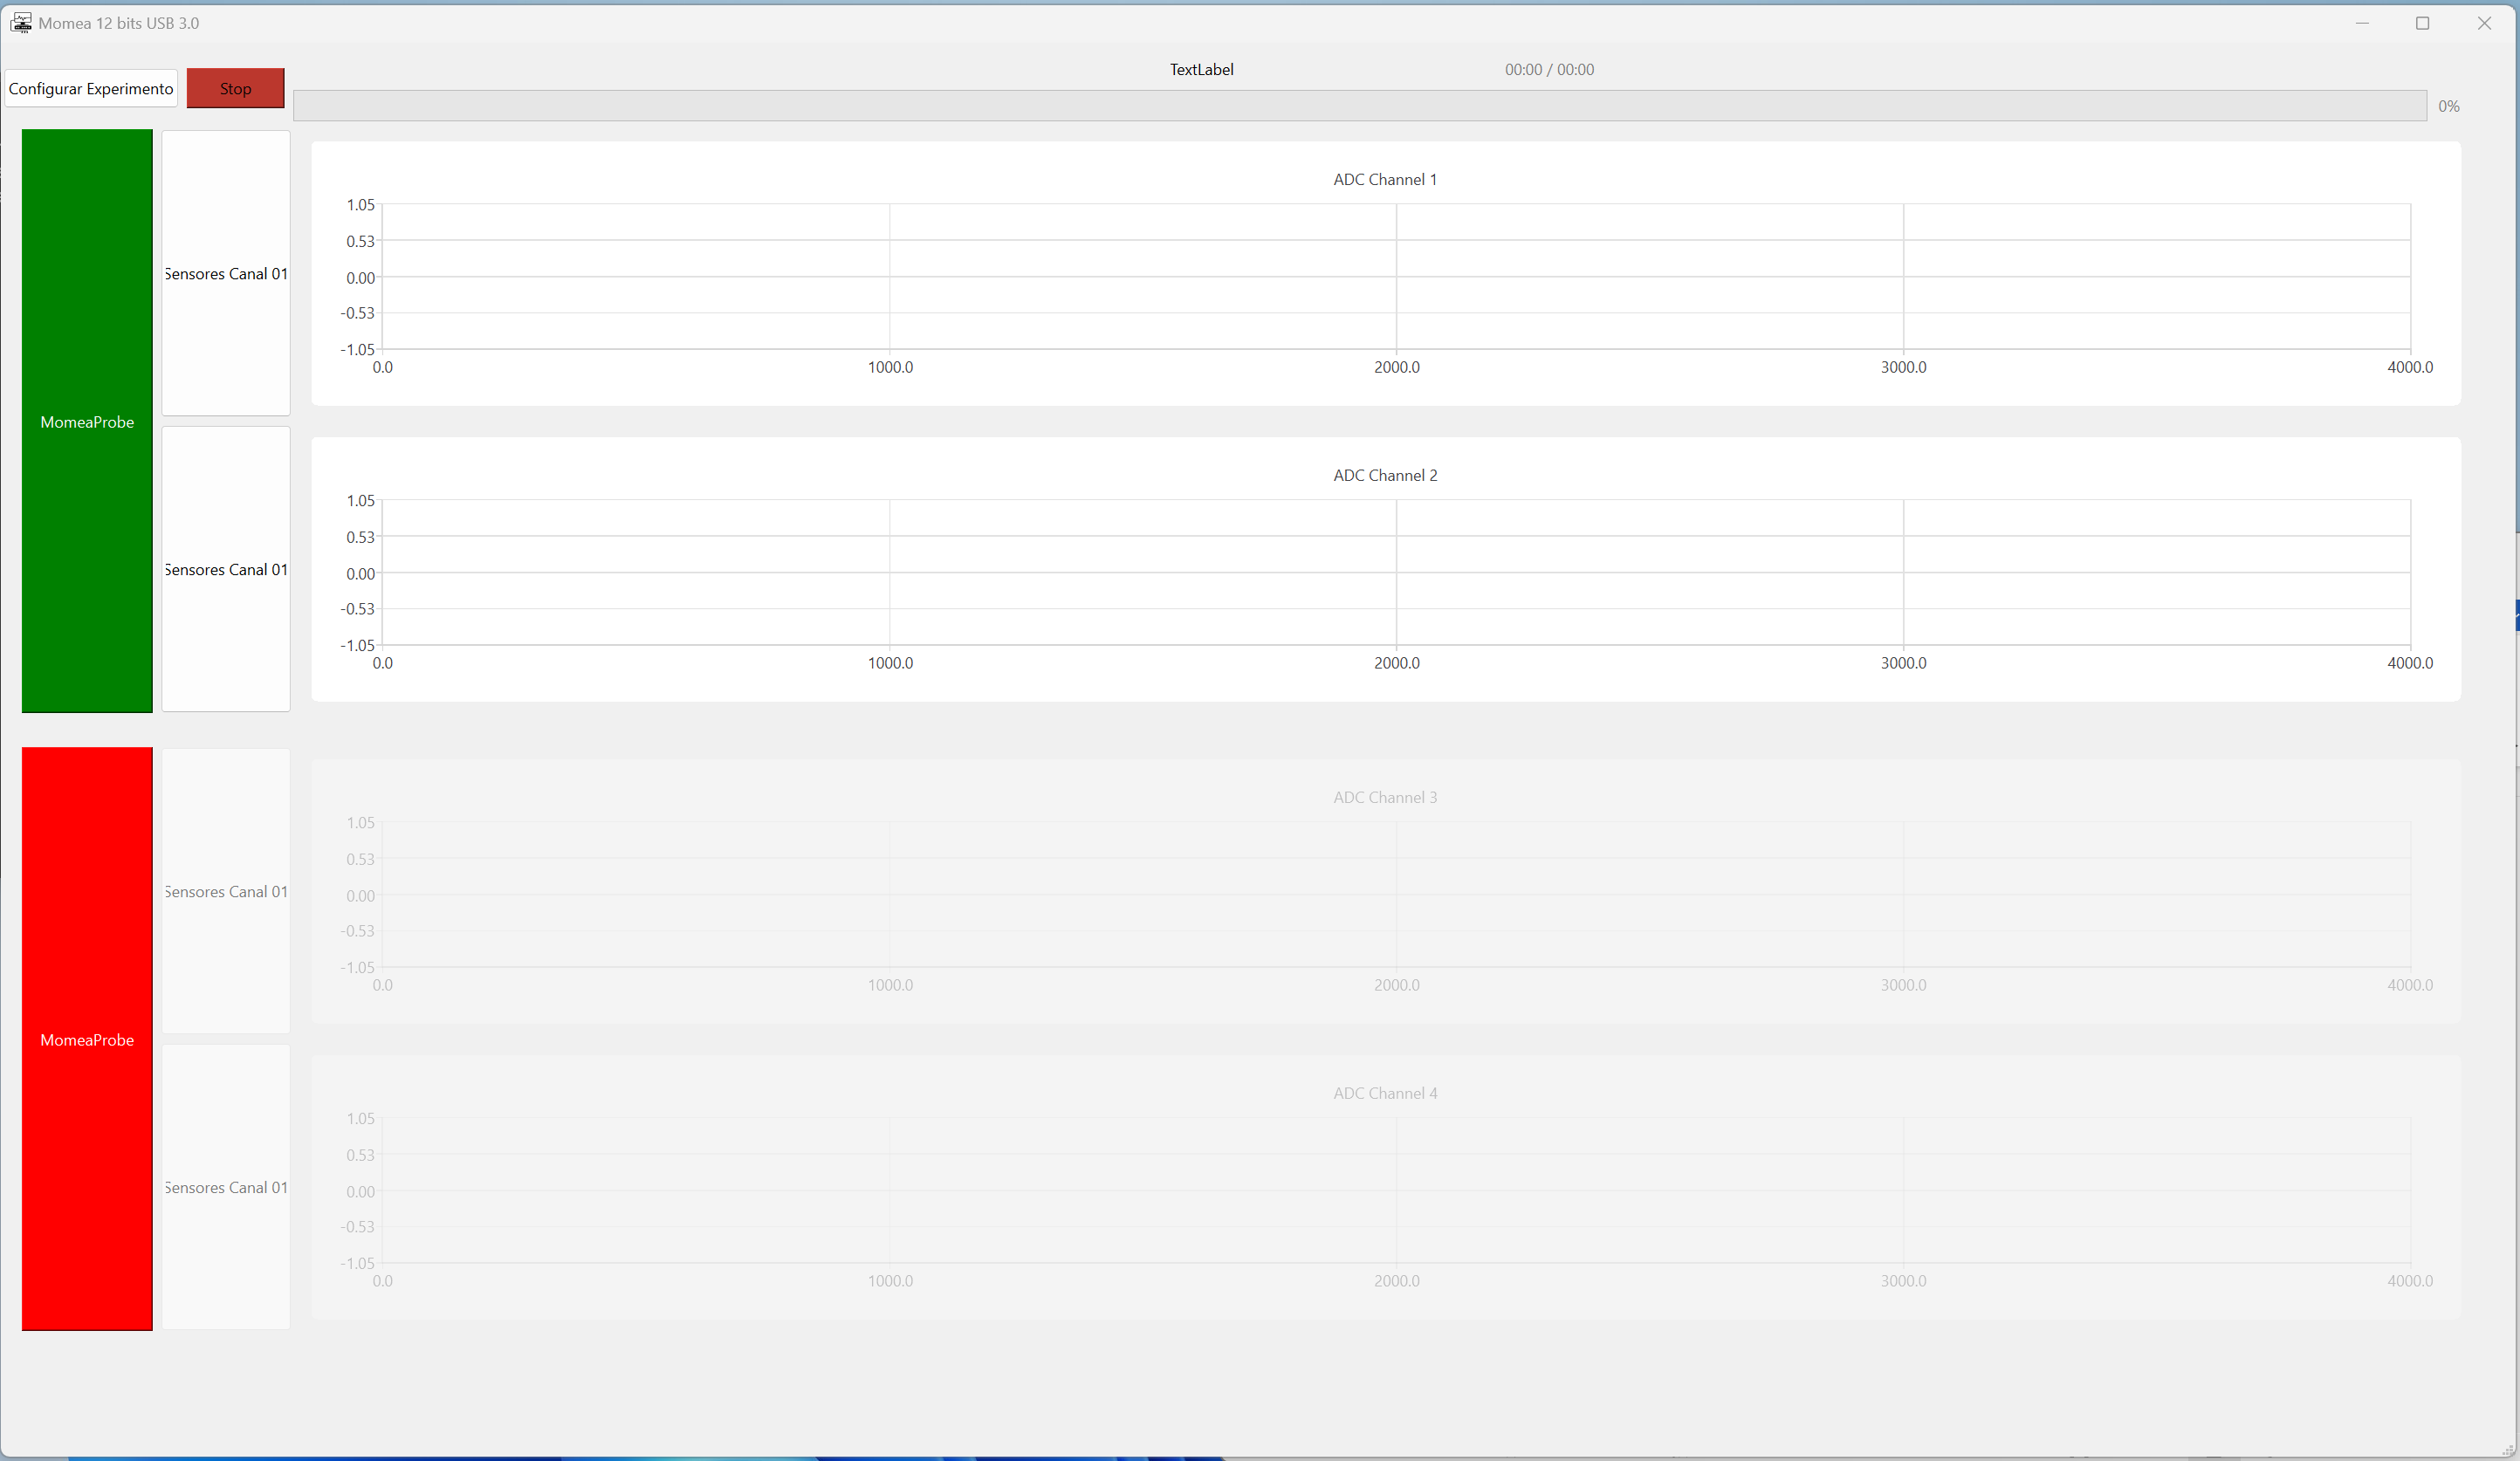
\includegraphics[width=\linewidth]{figs/MomeaCapture.png}
		\caption{Aplicação MomeaCapture.}
		\label{fig:MomeaCapture}
	\end{subfigure}
	\caption{Plataforma de aquisição contínua que antecedeu este trabalho. Fonte: o autor.}
	\label{fig:momea_usb}
\end{figure}

O uso dessa plataforma evidenciou o problema que motivou esta dissertação. A 8 a 10\,MSa/s por canal, com 12 a 16 bits por amostra, cada canal produz de 16 a 20\,MB/s, isto é, dezenas de gigabytes por hora. Manter esse fluxo exigiu, no computador, aquisição em múltiplas \textit{threads}, \textit{buffers} circulares, compactação contínua (LZMA) e escrita de alta vazão em disco. Na Figura~\ref{fig:MomeaUSB}, os dados brutos atravessam todo o caminho até a aplicação e só então são segmentados e analisados, de modo que a análise ocorre depois da gravação, e não em tempo real. A maior parte desse volume corresponde a ruído de fundo entre os eventos de interesse, que são esparsos.

\begin{figure}[htbp]
	\centering
	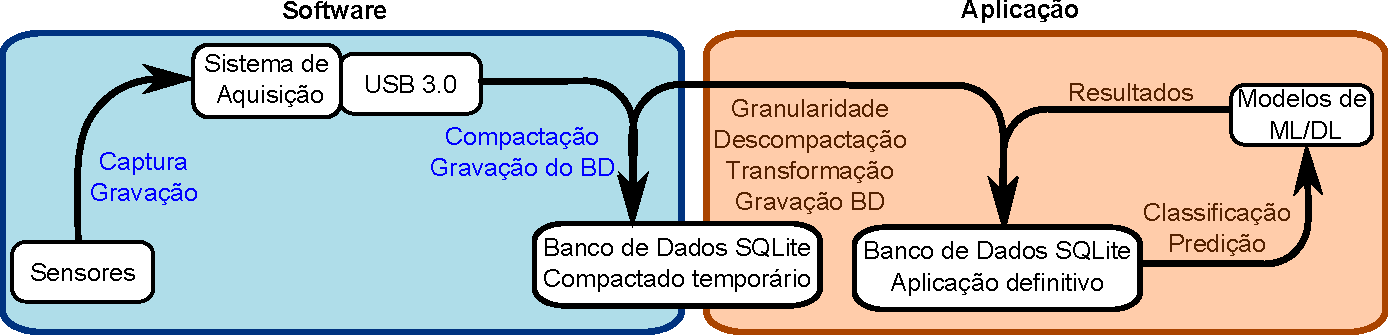
\includegraphics[width=0.95\linewidth]{figs/FluxoOperacaoMOMEAUSB}
	\caption[Fluxo de operação do sistema Momea USB]{Fluxo de operação do sistema MOMEA com aquisição contínua por USB: os dados brutos são compactados, armazenados em um banco temporário e só depois processados pela aplicação. Fonte: o autor.}
	\label{fig:MomeaUSB}
\end{figure}

A proposta desta dissertação desloca a redução de dados para antes da transmissão (Figura~\ref{fig:MomeaFPGA}): o FPGA detecta e parametriza os \textit{hits}, e apenas os registros seguem para a aplicação, por Ethernet a 100\,Mb/s. O destaque da figura é a diferença em relação ao fluxo USB: o bloco ``FPGA + HIT'' substitui a transmissão contínua de amostras, e a etapa de compactação deixa de ser necessária. As decisões que levaram a essa arquitetura são detalhadas a seguir.

\begin{figure}[htbp]
	\centering
	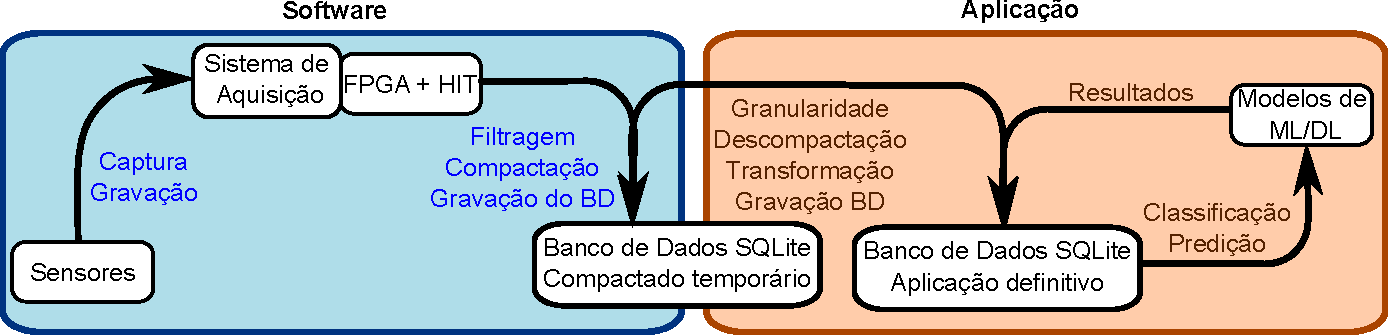
\includegraphics[width=0.9\linewidth]{figs/FluxoOperacaoMOMEAFPGA}
	\caption[Fluxo de operação do sistema Momea FPGA]{Fluxo de operação do sistema MOMEA com extração de \textit{hits} no FPGA. Em relação à Figura~\ref{fig:MomeaUSB}, o bloco ``FPGA + HIT'' (destacado) substitui a transmissão contínua das amostras. Fonte: o autor.}
	\label{fig:MomeaFPGA}
\end{figure}

% -------------------------------------------------------------------------------------------------------
\section{Arquitetura proposta: decisões de projeto}
\label{sec:mm_decisoes}
% Gerado por ferramentas/importar_relatorios.py a partir de ARTIGO_V2-10.11.2026/3-Decisoes_tecnologicas_metodologicas2.tex.
% Revisado à mão na dissertação: edite este arquivo, não a fonte.
% =======================================================================================================

Esta seção apresenta os requisitos e as decisões que conduziram à arquitetura adotada. A exposição é organizada segundo a relação requisito--alternativa--decisão--evidência, e não segundo a cronologia do desenvolvimento. O objetivo é explicitar os compromissos envolvidos e estabelecer quais resultados devem sustentar cada escolha nas Seções~\ref{sec:mm_implementacao} a~6.

% -------------------------------------------------------------------------------------------------------
\subsection{Requisitos e critérios de avaliação}
\label{v2:subsec:requisitos_arquitetura}

O cenário considerado é o monitoramento contínuo, distribuído e de longo prazo de sinais de EA. Nesse contexto, uma decisão de projeto somente pode ser considerada justificada quando o requisito correspondente é associado a um critério verificável. A Tabela~\ref{v2:tab:requisitos_sistema} resume os requisitos adotados e as evidências necessárias. Todavia, algumas informações são obtidas somente quando da realização dos ensaios, que são discutidos na Seção~\ref{sec:res_extrator}.

\begingroup
\footnotesize
\renewcommand{\arraystretch}{1.25}
\begin{longtable}{
		|>{\raggedright\arraybackslash}p{0.25\textwidth}
		|>{\raggedright\arraybackslash}p{0.34\textwidth}
		|>{\raggedright\arraybackslash}p{0.34\textwidth}|}
	\caption{Requisitos do sistema e respectivos valores quantitativos estabelecidos.}
	\label{v2:tab:requisitos_sistema}\\
	\hline
	\textbf{Requisito} & \textbf{Valor / meta} & \textbf{Situação} \\
	\hline
	\endfirsthead
	\multicolumn{3}{c}
	{\tablename\ \thetable{} -- continuação}\\
	\hline
	\textbf{Requisito} & \textbf{Valor / meta} & \textbf{Situação} \\
	\hline
	\endhead
	\hline
	\multicolumn{3}{r}{Continua na próxima página.}\\
	\endfoot
	\hline
	\endlastfoot
	Número de canais & 2 (dois canais independentes, A e B) & Definido \\
	\hline
	Taxa de amostragem efetiva & 10 MSa/s por canal ($\Delta t = 100$ ns) & Definido \\
	\hline
	Resolução do ADC & 12 bits + 1 bit de sobretensão por canal & Definido \\
	\hline
	Maior taxa sustentada de hits & Testada até 333 hits/s por canal (10\,000 \textit{bursts} em 30\,s), sem perda na comunicação (0/48\,280 registros) & Ensaio executado em 15/10/2026 (Seção~\ref{sec:res_extrator}); valor preliminar \\
	\hline
	Duração da rajada suportada & A medir (função da profundidade da FIFO/DMA) & Não ensaiada: com HLT de 2000\,\(\mu\)s cada \textit{hit} ocupa o canal por 2,27 a 2,44\,ms, e intervalos bem menores que 3\,ms exigem HLT reduzido e gerador com sequenciamento interno de rajadas \\
	\hline
	Latência admissível & A medir (caminho FSM$\to$DMA$\to$UDP$\to$receptor); mínimo de \(T_{\mathrm{HDT}} + T_{\mathrm{HLT}} = 2{,}25\,\mathrm{ms}\) após o último cruzamento & Não medida: a distribuição pedida exige instrumento com estatística de intervalos (Seção~\ref{sec:res_extrator}) \\
	\hline
	Erro máximo por descritor ($\tau_x$) & Valores iniciais propostos (Tabela~\ref{v2:tab:tau_x_iniciais}) & Metodológico; congelar antes da análise final \\
	\hline
	Custo-alvo por ponto & A consolidar (BOM do ponto completo) & A consolidar \\
\end{longtable}
\endgroup

Na versão submetida aos ensaios, o sistema tem dois canais a 10\,MSa/s e sustentou até 333 \textit{hits}/s por canal sem perda; os demais valores quantitativos são apresentados nas Seções~\ref{sec:mm_implementacao} e~\ref{sec:res_extrator}. 
% -------------------------------------------------------------------------------------------------------
\subsection{Arquitetura inicial baseada em \textit{streaming} contínuo}
\label{v2:subsec:streaming_continuo}

A plataforma inicialmente desenvolvida no Projeto MOMEA, denominada MOMEA-USB, transferia integralmente as amostras digitalizadas para um computador hospedeiro. O módulo de aquisição empregava dois conversores A/D com resolução nominal de 12 bits e taxa de amostragem de \(8\,\mathrm{MS/s}\) por canal, com transmissão por USB~3.0. A aplicação hospedeira, desenvolvida em C++ com o \textit{framework} Qt, realizava a recepção, a bufferização, o armazenamento e o processamento dos dados. 

O MOMEA-USB transporta os dois canais combinados em uma palavra de 32 bits, organizada como: 12 bits de dado + 1 bit de sobretensão + 3 bits de padding (canal A) e o mesmo arranjo para o canal B -- totalizando 16 bits por canal alinhados por byte -- e não empacotamento contínuo de 12 bits. Aplica-se compressão LZMA no nível 3 (a escala vai de 0 a 9), obtendo uma razão de compressão de aproximadamente 60\% em média (isto é, o arquivo comprimido fica em torno de 60\% do tamanho original).

A taxa associada às amostras depende do formato utilizado no transporte. Para \(N_{\mathrm{c}}\) canais, taxa \(f_{\mathrm{s}}\) e \(b_{\mathrm{tr}}\) bits transportados por amostra, a taxa sem sobrecargas é:
\begin{equation}
	R_{\mathrm{stream}} = N_{\mathrm{c}}f_{\mathrm{s}} \frac{b_{\mathrm{tr}}}{8}
	\label{v2:eq:taxa_streaming_secao3}
\end{equation}

Para dois canais a \(8\,\mathrm{MS/s}\), obtêm-se \(24\,\mathrm{MB/s}\) quando 12 bits são efetivamente empacotados e \(32\,\mathrm{MB/s}\) quando cada amostra ocupa uma palavra de 16 bits. Em aquisição ininterrupta, esses valores correspondem, respectivamente, a aproximadamente \(2{,}07\,\mathrm{TB/dia}\) e \(2{,}76\,\mathrm{TB/dia}\), antes de cabeçalhos, metadados, redundância e eventuais arquivos auxiliares.

Esses valores não mostram que o enlace USB~3.0, isoladamente, seja insuficiente. O desempenho depende da cadeia inteira, incluindo empacotamento, controlador USB, cópias em memória, escalonamento do sistema operacional, processamento, sistema de arquivos e unidade de armazenamento. A vazão sustentada medida foi de cerca de 28\,MB/s, sem perdas observadas. O sistema emprega um buffer circular de 1 GB, cuja ocupação máxima atingiu picos de cerca de 5\,\%. A aquisição durou 12 horas contínuas, a 8\,MSa/s, com compressão LZMA e sem perdas registradas pelos contadores. Assim, as limitações da arquitetura foram avaliadas por medições de vazão sustentada, ocupação dos \textit{buffers} e perdas, e não apenas pela taxa nominal da interface.

A arquitetura baseada em \textit{streaming} preserva o conjunto integral de amostras dentro dos limites de banda, resolução e ruído da cadeia. Isso mantém a possibilidade de aplicar posteriormente diferentes métodos de processamento ao mesmo registro. No cenário de operação contínua, entretanto, foram identificados três compromissos:

\begin{itemize}
	\item \textbf{Processamento e entrada/saída no computador hospedeiro:} a recepção sustentada exige bufferização, processamento concorrente e escrita com vazão suficiente. Por isso, neste trabalho, a ocorrência e a localização de perdas são demonstradas por contadores, e não inferidas de variações de desempenho.
	
	\item \textbf{Volume armazenado em relação à atividade de interesse:} em regimes esparsos, grande parte das amostras não pertence às janelas posteriormente identificadas como \textit{hits}. Essa fração depende do limiar, do DDT, da atividade observada e da definição da janela, devendo ser medida nos ensaios.
	
	\item \textbf{Latência variável:} as etapas de recepção, eventual compressão, armazenamento e análise introduzem atrasos dependentes da carga do hospedeiro e do subsistema de entrada e saída. Sem uma arquitetura de tempo real e uma análise de pior caso, não se deve atribuir limite determinístico a essa latência.
\end{itemize}

Esses compromissos não invalidam o \textit{streaming}. A preservação das formas de onda continua especialmente útil para caracterização de sinais, avaliação de novos algoritmos, investigação de 
ovo{eventos} não previstos e construção de bases de dados. A experiência com a MOMEA-USB motivou, porém, a avaliação de uma arquitetura em que o modo principal de operação transmite descritores extraídos localmente.

% -------------------------------------------------------------------------------------------------------
\subsection{Decisão pela extração de descritores na borda}
\label{v2:subsec:extracao_borda}

A arquitetura adotada desloca para o dispositivo de aquisição a detecção, a delimitação temporal e a extração dos descritores dos \textit{hits}. A decisão é adequada quando a informação requerida pelo nível superior pode ser representada por esses descritores e quando a taxa resultante é inferior à do fluxo de amostras.

Se \(\lambda_{\mathrm{h}}\) é a taxa total média de \textit{hits}, \(B_{\mathrm{reg}}\) é o tamanho do registro, \(m\) é o número médio de registros agregados por pacote, \(B_{\mathrm{ov}}\) é a sobrecarga por pacote referida ao ponto em que a vazão é avaliada e \(R_{\mathrm{aux}}\) reúne o tráfego de estado (keep-alive), comandos de configuração, mensagens de sincronização e retransmissões eventualmente implementadas, a taxa média pode ser aproximada por:
\begin{equation}
	R_{\mathrm{borda}} \approx \lambda_{\mathrm{h}}B_{\mathrm{reg}} + \frac{\lambda_{\mathrm{h}}}{m}B_{\mathrm{ov}} + R_{\mathrm{aux}}
	\label{v2:eq:taxa_borda}
\end{equation}

Todas as parcelas da Equação~\eqref{v2:eq:taxa_borda} devem ser expressas na mesma unidade, por exemplo, bytes por segundo. Para o registro de 256 bits descrito na Seção~\ref{sec:mm_implementacao}, \(B_{\mathrm{reg}}=32\) bytes, mas esse valor não inclui cabeçalhos, preenchimento, intervalo entre quadros nem retransmissões eventualmente implementadas pela aplicação. Na versão ensaiada, cada datagrama leva um único registro (\(m = 1\)), e a sobrecarga de Ethernet, IP e UDP é de 42 bytes por datagrama (46 com a sequência de verificação do quadro). A condição de redução de tráfego é
\begin{equation}
	R_{\mathrm{borda}} < R_{\mathrm{stream}}
	\label{v2:eq:condicao_reducao_borda}
\end{equation}

Desprezando a variação de \(R_{\mathrm{aux}}\) com a taxa de \textit{hits} (aproximação que deve ser verificada experimentalmente), a taxa aproximada de \textit{hits} no ponto de equilíbrio é:
\begin{equation}
	\lambda_{\mathrm{h,lim}} \approx \frac{R_{\mathrm{stream}}-R_{\mathrm{aux}}}{B_{\mathrm{reg}}+B_{\mathrm{ov}}/m}
	\label{v2:eq:taxa_limite_hits}
\end{equation}

Essa expressão evidencia que a redução não é uma constante da arquitetura. Ela depende da atividade detectada, do limiar, dos parâmetros temporais, do tamanho do registro, da agregação em pacotes e do tráfego auxiliar. A taxa de transmissão deixa de ser diretamente proporcional a \(N_{\mathrm{c}}f_{\mathrm{s}}\), mas a própria taxa de \textit{hits} ainda pode depender da amostragem, da banda e do detector.

O compromisso central é a não preservação integral da forma de onda no modo considerado. Após o descarte das amostras, não é possível recalcular os descritores com outro limiar ou outro DDT, aplicar retrospectivamente métodos baseados na forma de onda nem examinar 
ovo{eventos} não reconhecidos. A extração local é, portanto, uma transformação com perda de informação, e não uma compressão convencional com reconstrução do sinal.

Em atividade aproximadamente contínua ou sob ruído que produza muitos \textit{hits}, a vantagem de comunicação pode diminuir ou desaparecer. Além da taxa média, importa a maior rajada. Se a lógica produz registros à taxa \(\lambda_{\mathrm{in}}\), o software os retira à taxa de serviço \(\mu_{\mathrm{out}}\), e uma rajada com \(\lambda_{\mathrm{in}}>\mu_{\mathrm{out}}\) dura \(T_{\mathrm{b}}\), uma estimativa mínima para a capacidade adicional de fila é:
\begin{equation}
	C_{\mathrm{fila,min}} \geq \left(\lambda_{\mathrm{in}} - \mu_{\mathrm{out}}\right) T_{\mathrm{b}}
	\label{v2:eq:capacidade_fila_rajada}
\end{equation}

\noindent
expressa em número de registros. A validade dessa aproximação requer que as taxas sejam aproximadamente constantes durante a rajada. Quando a capacidade é excedida, o descarte é explícito e registrado por contadores de perda.

Um modo híbrido, com captura seletiva de formas de onda, pode reduzir a perda de flexibilidade analítica. Neste trabalho, esse modo não foi implementado e é tratado como extensão futura.

% -------------------------------------------------------------------------------------------------------
\subsection{Seleção da plataforma de hardware}
\label{v2:subsec:plataforma_hardware}

A seleção do hardware foi orientada pela execução contínua do caminho por amostra, pela necessidade de paralelismo nos filtros e acumuladores, pelas interfaces disponíveis, pelo custo por ponto e pela complexidade de integração. A Tabela~\ref{v2:tab:alternativas_arquitetura} resume as alternativas documentadas no desenvolvimento.

\begingroup
\footnotesize
\renewcommand{\arraystretch}{1.25}
\begin{longtable}
	{|>{\raggedright\arraybackslash}p{0.20\textwidth}
		|>{\raggedright\arraybackslash}p{0.25\textwidth}
		|>{\raggedright\arraybackslash}p{0.22\textwidth}
		|>{\raggedright\arraybackslash}p{0.20\textwidth}|}
	\caption{Alternativas arquiteturais consideradas e decisão adotada.}
	\label{v2:tab:alternativas_arquitetura}\\
	\hline
	\textbf{Alternativa} & \textbf{Vantagem preservada} & \textbf{Compromisso principal} & \textbf{Decisão} \\
	\hline
	\endfirsthead
	\multicolumn{4}{c}
	{\tablename\ \thetable{} -- continuação}\\
	\hline
	\textbf{Alternativa} & \textbf{Vantagem preservada} & \textbf{Compromisso principal} & \textbf{Decisão} \\
	\hline
	\endhead
	\hline
	\endlastfoot
	MOMEA-USB com processamento no hospedeiro & Forma de onda integral e grande flexibilidade de processamento posterior. & Vazão e armazenamento contínuos; dependência do hospedeiro; latência variável. & Linha de base. \\
	\hline
	Artix-7 com caminho de dados em lógica e MicroBlaze & Paralelismo por amostra, partição explícita entre dados e controle e ausência de processador \textit{hard} não utilizado. & O processador \textit{soft-core} e seus periféricos consomem recursos da lógica; rede e software continuam sujeitos a filas e variação temporal. & Selecionada. \\
	\hline
	Zynq-7000 com processador ARM integrado & Processador \textit{hard}, controladores e interfaces integrados ao sistema de processamento. & Complexidade de inicialização e integração entre PS e PL; eventual custo de recursos não exigidos pelo caminho crítico. & Considerada, não adotada. \\
\end{longtable}
\endgroup

O dispositivo selecionado foi o Artix-7 XC7A35T. A especificação da família informa \(33\,280\) células lógicas, \(5\,200\) \textit{slices}, 90 blocos DSP48E1 e \(1\,800\,\mathrm{Kb}\) de memória em blocos, equivalentes a 50 blocos de \(36\,\mathrm{Kb}\) \cite{xilinx2020ds180}. Como cada \textit{slice} da série 7 contém quatro LUTs e oito \textit{flip-flops}, o dispositivo oferece \(20\,800\) LUTs e \(41\,600\) registradores de \textit{slice}.

Esses números descrevem capacidade nominal, não suficiência para a aplicação. A decisão somente é sustentada pelos relatórios da versão implementada: utilização hierárquica de LUTs, registradores, BRAM e DSP; recursos de relógio e entrada/saída; potência estimada; e análise temporal pós-roteamento. O dispositivo é o Artix-7 XC7A35TICSG324-1L, encapsulamento CSG324, grau de velocidade -1L (baixa tensão, faixa industrial). A utilização e a análise temporal da versão implementada são apresentadas na Seção~\ref{sec:mm_implementacao} (Tabela~\ref{v2:tab:utilizacao_pos_implementacao}). 

A margem de recursos precisa ser avaliada em conjunto com a temporização e a largura de banda interna: baixa ocupação não garante que novos módulos possam ser acrescentados sem comprometer o fechamento temporal.

A família Zynq-7000 combina lógica programável e sistema de processamento baseado em ARM Cortex-A9 \cite{xilinx2018ds190}. No sistema proposto, o caminho por amostra é executado na lógica e as funções de controle possuem taxa inferior. Embora o Zynq pudesse oferecer maior desempenho de software, a complexidade adicional de inicialização e integração entre PS e PL não se justificava para as funções de controle requeridas, que são de baixa taxa e podem ser atendidas pelo MicroBlaze. Essa justificativa não demonstra superioridade geral do Artix-7: ela é válida para a partição adotada e deve ser complementada por comparação de custo, consumo, recursos e esforço de integração.

O argumento econômico deve considerar o ponto de medição completo. A comparação deve incluir placa de processamento, conversão A/D, condicionamento analógico, memória, comunicação, alimentação, conectores e proteções. Valores monetários devem trazer data, quantidade, moeda e natureza do item---placa de desenvolvimento, protótipo ou estimativa de produção.

% -------------------------------------------------------------------------------------------------------
\subsection{Partição entre lógica programável e software embarcado}
\label{v2:subsec:divisao_hw_sw}

A arquitetura separa o caminho de dados, executado na taxa das amostras, do caminho de controle, executado na taxa de geração e transmissão dos registros. Essa partição é resumida na Tabela~\ref{v2:tab:particao_hw_sw}.
\begin{table}[htbp]
	\centering
	\footnotesize
	\caption{Partição funcional entre lógica programável e software.}
	\label{v2:tab:particao_hw_sw}
	\renewcommand{\arraystretch}{1.25}
	\begin{tabular}
		{|>{\raggedright\arraybackslash}p{0.22\textwidth}
			|>{\raggedright\arraybackslash}p{0.35\textwidth}
			|>{\raggedright\arraybackslash}p{0.35\textwidth}|}
		\hline
		\textbf{Camada} & \textbf{Funções} & \textbf{Condição de desempenho} \\ 
		\hline
		Lógica programável & Recepção das amostras, filtragem, limiar, máquina de estados, pico, contagens e acumuladores. & Fechamento temporal; ausência de bloqueio no caminho por amostra; tratamento explícito de transbordos e cruzamentos de domínio. \\
		\hline
		MicroBlaze e FreeRTOS & Configuração, retirada e empacotamento dos registros, pilha de comunicação, comandos e informações de estado. & Tempo de serviço superior à taxa média de entrada; prioridades e filas dimensionadas para a rajada especificada. \\
		\hline
		Computador ou nível superior & Recepção, verificação de sequência, persistência, visualização e análise posterior. & Detecção de perdas, tratamento de reordenação e preservação dos metadados de configuração e sincronização. \\
		\hline
	\end{tabular}
\end{table}

A implementação em lógica explora paralelismo e produz uma latência de \textit{pipeline} expressa por número definido de ciclos, desde que todas as restrições temporais sejam satisfeitas e o caminho não seja interrompido por contenção ou contrapressão. Isso não torna fixa a latência de emissão do registro: o registro somente pode ser consolidado depois do último cruzamento e da expiração do DDT.

O MicroBlaze executa FreeRTOS para organizar tarefas assíncronas de comunicação e configuração. O escalonamento preemptivo facilita a atribuição de prioridades, mas não garante, isoladamente, ausência de perda ou prazo de resposta. Da arquitetura tem-se: processador soft-core MicroBlaze executando FreeRTOS e pilha lwIP, com transferência dos registros por DMA e transmissão UDP. Quando da pós-implementação será discutida a frequência do processador, as prioridades das tarefas, os tempos máximos de execução, as interrupções, a profundidade das filas, a política de \textit{cache} e o mecanismo de coerência com o DMA, quando aplicável.

Se a latência for medida desde a entrada da amostra correspondente ao primeiro cruzamento até a disponibilização do registro no receptor, uma decomposição apropriada é \(L_{\mathrm{total}} = L_{\mathrm{pipe}} + t_{\mathrm{dur}} + T_{\mathrm{DDT,impl}} + L_{\mathrm{fin}} + L_{\mathrm{fila}} + L_{\mathrm{SW}} + L_{\mathrm{rede}}\), em que \(L_{\mathrm{pipe}}\) é a latência até a decisão correspondente, \(t_{\mathrm{dur}}\) é a duração entre primeiro e último cruzamentos, \(L_{\mathrm{fin}}\) é a finalização do registro na lógica e as três últimas parcelas representam fila, software e rede. Se a referência temporal for o último cruzamento, o termo \(t_{\mathrm{dur}}\) deve ser omitido. Apenas \(L_{\mathrm{pipe}}\), \(T_{\mathrm{DDT,impl}}\) e \(L_{\mathrm{fin}}\) podem ser associados diretamente a quantidades determinadas de ciclos; as demais parcelas dependem da carga.

% -------------------------------------------------------------------------------------------------------
\subsection{Comunicação, observabilidade de perdas e sincronização}
\label{v2:subsec:interface_comunicacao}

Adotou-se Ethernet 10/100 para desacoplar o ponto de aquisição de uma conexão USB direta e permitir sua integração a uma rede comutada. No modo de \(100\,\mathrm{Mb/s}\), a taxa nominal do enlace equivale a \(12{,}5\,\mathrm{MB/s}\); no modo de \(10\,\mathrm{Mb/s}\), equivale a \(1{,}25\,\mathrm{MB/s}\). A vazão útil é menor devido aos cabeçalhos, ao preenchimento, ao preâmbulo e ao intervalo entre quadros. Nos ensaios, o enlace operou no modo de 100\,Mb/s. 

Para taxa de pacotes \(\lambda_{\mathrm{p}}\), conteúdo útil médio \(B_{\mathrm{payload}}\) e sobrecarga por pacote \(B_{\mathrm{ov,rede}}\), a taxa no enlace pode ser estimada por 
\begin{equation}
	R_{\mathrm{rede}} \approx 8\lambda_{\mathrm{p}} \left(B_{\mathrm{payload}} + B_{\mathrm{ov,rede}}\right)
	\label{v2:eq:taxa_rede}
\end{equation}

\noindent
em bits por segundo. A definição de \(B_{\mathrm{ov,rede}}\) deve indicar se a medição considera apenas UDP/IP, o quadro Ethernet ou todos os elementos transmitidos no meio físico.

Os registros são transportados por UDP. Esse protocolo reduz o estado e os mecanismos do transporte, mas não garante entrega, ordenação nem proteção contra duplicação \cite{postel1980udp}. A decisão por UDP deve, portanto, ser acompanhada na camada de aplicação por número sequencial de pacotes, quantidade de registros por pacote, contador cumulativo de registros produzidos e indicação de reinicialização. 

O cabeçalho de aplicação com versão do protocolo, identificação do dispositivo, número de sequência, quantidade de registros, contador cumulativo, carimbo de tempo de referência, tamanho do conteúdo e indicadores de erro ou reinicialização foi especificado, mas não implementado na versão ensaiada. Cada datagrama da porta 5007 leva apenas os 32 bytes de um registro de \textit{hit}, sem cabeçalho de aplicação nem número de sequência gerado no dispositivo. Na versão ensaiada, a observabilidade de perdas é obtida por contadores independentes em cada etapa: na lógica, o contador \texttt{HITCNT} (\textit{hits}, ROVL e MAXDUR por canal) e os registradores de depuração do mapa AXI; no firmware, os contadores de transferências do DMA e de falhas de envio; e, no receptor, a numeração dos datagramas e dos registros na chegada. Ao fim de cada captura, o \textit{software} de aquisição compara o total de registros contado na lógica com o total recebido e gravado, de modo que \(N_{\mathrm{perdidos}} = N_{\mathrm{HITCNT}} - N_{\mathrm{rx}}\). Duplicações e trocas de ordem não são detectáveis individualmente sem número de sequência; o risco é reduzido pelo enlace direto entre a placa e o computador, sem comutadores. O cabeçalho especificado permanece como evolução prevista, e o campo de 32 bits livre no registro é candidato a número de sequência.

A Ethernet também não fornece determinismo temporal nem qualificação industrial por si só. A robustez física depende de transceptor, isolamento, conectores, cabeamento, alimentação, proteção contra transientes e compatibilidade eletromagnética. A latência depende das filas, da pilha, do controlador, dos comutadores e da carga da rede.

Se registros de diferentes canais ou dispositivos forem correlacionados pelo tempo, deve existir mecanismo explícito de sincronização. A arquitetura prevista é um carimbo de tempo gerado por um contador livre no FPGA, com largura de 64 bits e resolução de 100 ns (um período de amostra a 10 MHz, igual à grade do AMSY-6), com época zerada nos comandos START e STOP. O campo correspondente já está reservado no registro do \textit{hit}, mas o \textit{bitstream} ensaiado o envia zerado. Como a conectividade Ethernet não estabelece base de tempo comum, a sincronização com o AMSY-6 prevista é um sinal de disparo do gerador aplicado às duas cadeias, com associação entre estímulos e \textit{hits} por janelas temporais em torno de cada disparo. Sem o carimbo, essa associação \textit{hit} a \textit{hit} e a medição da deriva entre as bases de tempo não são possíveis; nos ensaios desta etapa, a associação foi feita por bloco de estímulos.

% -------------------------------------------------------------------------------------------------------
\subsection{Verificação instrumental e validação no domínio de aplicação}
\label{v2:subsec:metodologia_validacao}

O trabalho distingue \textit{verificação instrumental} e \textit{validação no domínio de aplicação}. A primeira examina se a cadeia elétrica e digital implementa os descritores especificados. A segunda examina se o instrumento fornece informação útil para detectar ou caracterizar cavitação no ambiente de uso. As duas etapas respondem a perguntas diferentes e não são equivalentes.

\subsubsection{Estratégias experimentais}
Duas estratégias são complementares:

\begin{description}
	\item[Estímulo elétrico controlado:] um gerador produz formas de onda com amplitude, duração, frequência, fase e espaçamento configurados. A injeção após o sensor elimina da avaliação os efeitos do acoplamento e da propagação mecânica e é adequada para verificar aquisição, detecção e parametrização.
	
	\item[Ensaio de cavitação:] inclui o fenômeno físico, o sensor, o acoplamento, a estrutura e o ruído da máquina. É necessário para a validação no domínio, mas não isola com facilidade erros da eletrônica ou do algoritmo, pois as fontes físicas ativas não são diretamente conhecidas.
\end{description}

Este trabalho adota, nesta etapa, o estímulo elétrico controlado. Logo, suas conclusões limitam-se à parte da cadeia posterior ao ponto de injeção. O ensaio não valida sensor, acoplamento, propagação estrutural nem capacidade de discriminar cavitação em operação real.

\subsubsection{Hierarquia das referências}
Os valores configurados no gerador não constituem referência exata. Cabos, divisores, terminações, impedâncias de entrada e largura de banda modificam o sinal. A metodologia deve distinguir quatro níveis:

\begin{enumerate}
	\item Os valores nominais programados no gerador;
	
	\item A forma de onda efetivamente aplicada em um plano de referência elétrico, medida por instrumento independente com calibração, largura de banda, taxa de amostragem e incerteza conhecidas;
	
	\item Os descritores de referência calculados \textit{off-line} a partir dessa forma de onda, empregando as definições da Seção~\ref{sec:fund_hits} e convenções explícitas de amostragem, limiar e janela; e
	
	\item Os descritores do AMSY-6, utilizado como instrumento de comparação, mas não como 
ovo{referência primária}.
\end{enumerate}

A mesma forma de onda é aplicada simultaneamente às duas cadeias, por meio de um divisor cujas atenuação, largura de banda, isolamento e impedâncias precisam ser caracterizados; em ensaios sequenciais, a repetibilidade e a deriva do gerador entram na avaliação de incerteza. Os instrumentos são um gerador de sinais e um osciloscópio digital Minipa MVB DSO de 100\,MHz, usado como referência da forma de onda (nível 2 da hierarquia de referências), com as características da Tabela~\ref{v2:tab:instrumentos}.

\begingroup
\footnotesize
\renewcommand{\arraystretch}{1.25}
\begin{longtable}{
		|>{\raggedright\arraybackslash}p{0.19\textwidth}
		|>{\raggedright\arraybackslash}p{0.34\textwidth}
		|>{\raggedright\arraybackslash}p{0.38\textwidth}|}
	\caption{Instrumentos utilizados nos ensaios e respectivas especificações principais.}
	\label{v2:tab:instrumentos}\\
	\hline
	\textbf{Instrumento} & \textbf{Especificação} & \textbf{Valor / Observação} \\
	\hline
	\endfirsthead
	\multicolumn{3}{c}
	{\tablename\ \thetable{} -- continuação}\\
	\hline
	\textbf{Instrumento} & \textbf{Especificação} & \textbf{Valor / Observação} \\
	\hline
	\endhead
	\hline
	\multicolumn{3}{r}{Continua na próxima página.}\\
	\endfoot
	\hline
	\endlastfoot
	Osciloscópio digital & Modelo & Minipa, linha MVB DSO, 100 MHz \\
	\hline
	& Banda (upgrade) & 50 / 70 / 100 MHz \\
	\hline
	& Amostragem em tempo real & até 1 GSa/s \\
	\hline
	& Amostragem acumulativa & 50 GSa/s por canal (sinais repetitivos) \\
	\hline
	& Canais de entrada & 2 \\
	\hline
	& Base de tempo & 2 ns ~ 50 s/DIV \\
	\hline
	& Fator de deflexão vertical & 1 mV ~ 20 V/DIV \\
	\hline
	& Precisão vertical básica & 3\% \\
	\hline
	& Precisão horizontal básica & ±50 ppm \\
	\hline
	& Tempo de subida & 3,5 ns \\
	\hline
	& Tensão máxima de entrada & 400 V (DC + pico AC), 1 MHz \\
	\hline
	& Memória por canal & 25 kByte \\
	\hline
	Gerador de sinais & Modelo & Rigol DG832, 2 canais, 35 MHz \\
	\hline
	& Canais & 2 \\
	\hline
	& Frequência (seno) & 1 µHz ~ 35 MHz \\
	\hline
	& Taxa de amostragem & até 125 MSa/s \\
	\hline
	& Resolução vertical & 16 bits \\
	\hline
	& Profundidade de memória & 2 Mpts padrão (8 Mpts opcional) \\
	\hline
	& Estabilidade de frequência & ±1 ppm \\
	\hline
	& Ruído de fase & -105 dBc/Hz \\
	\hline
	& Jitter de saída & tão baixo quanto 200 ps \\
	\hline
	& Precisão de frequência & ±(1 ppm do ajuste + 10 µHz), 18--28 °C \\
	\hline
	& Formas de onda arbitrárias & até 160 integradas; edição por PC \\
	\hline
\end{longtable}
\endgroup

\subsubsection{Matriz de ensaios e critérios de aceitação}
A matriz de ensaios deve explorar não apenas condições nominais, mas também fronteiras que revelem diferenças de implementação:

\begin{itemize}
	\item Amplitudes próximas ao limiar e próximas à saturação;
	
	\item Diferentes frequências dentro da banda e próximas às frequências de corte;
	
	\item Durações e números de ciclos distintos; 
	
	\item Separações de \(N_{\mathrm{DDT}}-1\), \(N_{\mathrm{DDT}}\) e \(N_{\mathrm{DDT}}+1\) amostras;
	
	\item Condições comparáveis nas proximidades do RAT, quando houver comparação de cascatas; e
	
	\item Repetições suficientes para estimar dispersão, perdas e repetibilidade.
\end{itemize}

Para cada descritor \(x\), podem ser calculados o erro \(e_x = x_{\mathrm{prop}} - x_{\mathrm{ref}}\), e, quando \(x_{\mathrm{ref}}\) estiver suficientemente afastado de zero, o erro relativo
\begin{equation}
	e_{x,\mathrm{rel}} = \frac{x_{\mathrm{prop}}-x_{\mathrm{ref}}}{x_{\mathrm{ref}}}
	\label{v2:eq:erro_relativo_descritor}
\end{equation}

O erro relativo não é usado para referências nulas ou muito pequenas; nesses casos, usa-se o erro absoluto ou o desvio em unidades de resolução (LSB ou equivalente). Em ensaios repetidos, reportam-se viés, dispersão e intervalos de incerteza, além das taxas de detecção, perda e fragmentação. A avaliação de incerteza considera gerador, instrumento independente, divisor, ganho, resolução temporal, quantização e repetibilidade, seguindo princípios compatíveis com o JCGM~100 \cite{jcgm2008}.

Os limites de aceitação devem ser definidos antes da interpretação dos resultados e relacionados à resolução e à incerteza de cada descritor. Os valores iniciais de \(\tau_x\) da Tabela~\ref{v2:tab:tau_x_iniciais} partem da resolução de cada descritor e das componentes de incerteza descritas na Seção~\ref{sec:mm_delineamento}. A base do AMSY-6 provém da especificação do fabricante, e a do sistema proposto, dos componentes da cadeia. A banda do osciloscópio de referência (100 MHz) é adequada, mas sua precisão vertical de 3\,\% é a maior componente de incerteza da referência de amplitude e, como a energia é proporcional ao quadrado da tensão, da referência de energia, cuja incerteza relativa é \(2 \times 3\,\% \approx 6\,\%\). A referência de tempo do osciloscópio (\(\pm 50\) ppm) é folgada para os descritores temporais. A coluna de repetibilidade traz o desvio-padrão medido no ensaio simultâneo de 15/10/2026 como dado de entrada, e não como critério escolhido a partir do resultado.

\begingroup
\footnotesize
\renewcommand{\arraystretch}{1.25}
\begin{longtable}{
		|>{\raggedright\arraybackslash}p{0.11\textwidth}
		|>{\raggedright\arraybackslash}p{0.21\textwidth}
		|>{\raggedright\arraybackslash}p{0.15\textwidth}
		|>{\raggedright\arraybackslash}p{0.17\textwidth}
		|>{\raggedright\arraybackslash}p{0.22\textwidth}|}
	\caption{Valores iniciais propostos para as tolerâncias \(\tau_x\).}
	\label{v2:tab:tau_x_iniciais}\\
	\hline
	\textbf{Descritor} & \textbf{Base no sistema proposto (componentes)} & \textbf{Base no AMSY-6 (fabricante)} & \textbf{Repetibilidade medida no sistema proposto (15/10)} & \textbf{\(\tau_x\) inicial proposto} \\
	\hline
	\endfirsthead
	\hline
	\textbf{Descritor} & \textbf{Base no sistema proposto} & \textbf{Base no AMSY-6} & \textbf{Repetibilidade} & \textbf{\(\tau_x\) inicial} \\
	\hline
	\endhead
	\hline
	\endlastfoot
	Amplitude & 1 LSB referido à entrada (3,13--3,23\,mV no ADC) + incerteza do ganho do pré-amplificador (34,00\,dB medidos) & Não informada na especificação consultada & \(\sigma = 0{,}04\)--\(0{,}06\)\,dB & \(\pm\)(1 LSB + \(u\) do ganho); contra a referência do osciloscópio, \(\pm 3\,\%\) (\(0{,}26\)\,dB) \\
	\hline
	Tempo de subida & 1 amostra (100\,ns) + fase do \textit{burst} em relação à grade de 10\,MHz & Resolução de 100\,ns (ASIP-2 a 10\,MHz) & Não aplicável com envelope retangular (pico ambíguo) & \(\pm 1\) amostra + \textit{jitter} de fase; avaliado só com envelope realista \\
	\hline
	Duração & 1--2 amostras (100--200\,ns) + convenção de término & 100\,ns & \(\sigma = 0{,}04\)--\(0{,}06\,\mu\)s & \(\pm 2\) amostras; comparação com o AMSY-6 apenas como descritor assemelhado \\
	\hline
	Contagens & Discreto; depende do limiar e do sinal de decisão & Discreto & Constante (10) em 48\,197 de 48\,198 \textit{hits} & \(\pm 1\) \\
	\hline
	Energia & \(2\times\) a incerteza relativa da amplitude (entra ao quadrado) & Definição de eu do fabricante & 0,12--0,64\,\% (desvio relativo) & \(\pm 6\,\%\) contra a referência; comparação com o AMSY-6 apenas como descritor assemelhado \\
\end{longtable}
\endgroup

 Uma forma geral é:
\begin{equation}
	\left|x_{\mathrm{prop}} - x_{\mathrm{ref}} \right| \leq \tau_x
	\label{v2:eq:criterio_aceitacao_descritor}
\end{equation}

\noindent
em que \(\tau_x\) é a tolerância previamente estabelecida. A comparação com o AMSY-6 avalia concordância entre implementações; a comparação com os descritores derivados da forma de onda medida fornece referência independente. Nenhuma das duas substitui a posterior validação em uma bancada de cavitação.
% =======================================================================================================


% -------------------------------------------------------------------------------------------------------
\section{Implementação do extrator de \textit{hits}}
\label{sec:mm_implementacao}
% Gerado por ferramentas/importar_relatorios.py a partir de ARTIGO_V2-10.11.2026/4-Implementacao_sistema2.tex.
% Revisado à mão na dissertação: edite este arquivo, não a fonte.
% =======================================================================================================

Esta seção descreve a implementação da cadeia de aquisição, detecção, parametrização e transmissão dos registros de \textit{hits}. O protótipo avaliado nos ensaios da Seção~\ref{sec:res_extrator} foi construído segundo a arquitetura descrita a seguir. A exposição distingue os elementos confirmados no protótipo das informações que ainda dependem de verificação final no esquemático, no código-fonte e nos relatórios das ferramentas de desenvolvimento.

% -------------------------------------------------------------------------------------------------------
\subsection{Visão geral da arquitetura}
\label{v2:subsec:visao_geral_arquitetura}

O sistema adota uma organização funcional comparável à encontrada em instrumentos de EA, sem pretender reproduzir integralmente a arquitetura interna de um equipamento comercial. A cadeia compreende sensor, pré-amplificação, filtragem e ganho analógicos, conversão A/D, processamento em lógica programável, software embarcado e comunicação Ethernet.

\begin{figure}[htbp]
	\centering
	\IfFileExists{figuras/arquitetura_geral_sistema.pdf}
	{
		\includegraphics[width=\textwidth]
		{figuras/arquitetura_geral_sistema.pdf}
	}
	{
		\fbox{
			\parbox[c][4.0cm][c]{0.92\textwidth}{
				\centering
				\textbf{Diagrama da arquitetura}\\[0.3cm] (arquivo \texttt{figuras/arquitetura\_geral\_sistema.pdf})
				
			}
		}
	}
	\caption{Arquitetura geral do sistema embarcado de aquisição, detecção e parametrização de \textit{hits} de emissão acústica.}
	\label{v2:fig:arquitetura_geral}
\end{figure}

No domínio analógico, o sinal proveniente do sensor é amplificado e limitado em banda antes de ser adequado à faixa de entrada do conversor. O filtro analógico participa da rejeição das componentes que poderiam sofrer \textit{aliasing}; essa função não pode ser transferida integralmente para o processamento digital, pois componentes já sobrepostas à banda útil após a amostragem não podem ser separadas posteriormente.

No domínio digital, a lógica programável recebe as amostras, executa a filtragem, compara o sinal processado com o limiar, delimita os \textit{hits} e acumula seus descritores. Os registros consolidados são encaminhados ao subsistema com MicroBlaze e FreeRTOS, que realiza a retirada, o empacotamento, o atendimento aos comandos de configuração e a transmissão por UDP.

As interfaces da versão ensaiada, com largura, taxa, relógio e controle de fluxo, são:
\begin{itemize}
	\item ADC AD9226 \(\rightarrow\) \texttt{adc12\_frontend}: 2 canais \(\times\) 12 bits + OTR, 10\,MSa/s, relógio de 10\,MHz gerado por MMCM;
	\item filtro IIR (\texttt{adc\_ctrl\_axi} / \texttt{iir\_biquad\_df2}): Butterworth passa-baixas de 4ª ordem (2 \textit{biquads}), coeficientes Q3.17 de 20 bits, domínio de 100\,MHz;
	\item extrator (\texttt{ae\_hit\_extractor} rev 0.08, dentro do \texttt{ae\_hit\_axi\_wrapper} rev 0.08) \(\rightarrow\) \texttt{hit\_to\_axis} rev 0.07: palavra de 256 bits, AXI-Stream com TLAST ao fim de cada \textit{hit};
	\item \texttt{axis\_data\_fifo} \(\rightarrow\) AXI DMA (S2MM, modo simples) \(\rightarrow\) DDR3 pelo controlador MIG (interface a 81,25\,MHz; referência de 200\,MHz);
	\item MicroBlaze + FreeRTOS + lwIP (100\,MHz) \(\rightarrow\) AXI Ethernet Lite (PHY a 25\,MHz) \(\rightarrow\) UDP: comandos na porta 5006 e registros na porta 5007;
	\item controle de fluxo: sinal \texttt{tready} do AXI-Stream; estouro da FIFO sinalizado por \texttt{overflow\_out} do \texttt{hit\_to\_axis}.
\end{itemize}

% -------------------------------------------------------------------------------------------------------
\subsection{\textit{Front-end} analógico}
\label{v2:subsec:front_end_analogico}

O \textit{front-end} analógico realiza o acoplamento elétrico com o sensor, a amplificação, a limitação de banda e a adequação do sinal à entrada do conversor A/D. São utilizados dois sensores Vallen: o VS45-H (sensor de baixa frequência, faixa nominal 30–100 kHz) e o VS900-M (sensor de banda larga).

Em primeira aproximação e fora das regiões de ressonância, um sensor piezoelétrico pode ser representado por uma fonte de tensão associada a uma capacitância \(C_{\mathrm{s}}\). Sua impedância é, portanto, dependente da frequência:
\begin{equation}
	Z_{\mathrm{s}}(f)
	\approx
	\frac{1}{j2\pi f C_{\mathrm{s}}},
	\label{v2:eq:impedancia_sensor}
\end{equation}
sendo utilizado apenas para ilustrar a dependência frequencial da impedância, e não como substituto da resposta eletromecânica completa do transdutor.

O pré-amplificador utilizado nos ensaios possui ganho de patamar medido de \(34{,}00\,\mathrm{dB}\), próximo do ganho nominal do pré-amplificador AEP5 usado com o AMSY-6 (34\,dB). A descrição anterior deste texto (três amplificadores AD8065, com \textit{buffer} seguido de dois estágios de ganho 10, totalizando 40\,dB nominais) não corresponde ao circuito efetivamente ensaiado.

Ganho e banda foram medidos por varredura de 1\,kHz a 35\,MHz, com 100\,mVpp injetados pelo gerador e saída lida no osciloscópio de referência, na mesma montagem de cabos RG59 e divisor usada nos ensaios. Os resultados estão na Tabela~\ref{v2:tab:preamp_medido}. A versão original do circuito tinha corte superior em \(\approx 0{,}99\,\mathrm{MHz}\), abaixo da meta de 2\,MHz; a modificação do circuito levou o corte para \(\approx 2{,}5\,\mathrm{MHz}\), sem saturação na faixa. Também foi eliminada a oscilação de 43\,MHz que surgia no \textit{buffer} de entrada com o cabo do sensor conectado: o resistor de isolação na entrada passou de \(100\,\Omega\) para \(1\,\mathrm{k}\Omega\).

\begin{table}[htbp]
	\centering
	\footnotesize
		\caption{Ganho e banda medidos dos pré-amplificadores.}
	\label{v2:tab:preamp_medido}
	\begin{tabular}{|p{0.30\textwidth}|p{0.14\textwidth}|p{0.16\textwidth}|p{0.26\textwidth}|}
		\hline
		\textbf{Pré-amplificador} & \textbf{Ganho de patamar} & \textbf{Corte superior (\(-3\,\mathrm{dB}\))} & \textbf{Observação} \\
		\hline
		Sistema proposto, versão original & 33,90\,dB & \(\approx 0{,}99\,\mathrm{MHz}\) & Abaixo da meta de 2\,MHz \\
		\hline
		Sistema proposto, após modificação (usado nos ensaios) & 34,00\,dB & \(\approx 2{,}50\,\mathrm{MHz}\) & Atende a meta de 2\,MHz; sem saturação na faixa \\
		\hline
		Vallen AEP5 (referência) & 34,22\,dB & \(\approx 4{,}10\,\mathrm{MHz}\) & Próximo do nominal de 34\,dB \\
		\hline
	\end{tabular}
\end{table}

Todas as conversões entre \(\mathrm{dB}_{\mathrm{AE}}\) e códigos do ADC usam o ganho de 34\,dB: por exemplo, o limiar de \(80\,\mathrm{dB}_{\mathrm{AE}}\) corresponde a 155 códigos, ou \(\approx 0{,}50\,\mathrm{V}\) na entrada da placa.

O AD8065 é um amplificador de realimentação de tensão com entrada FET. A documentação informa, entre outros valores típicos, corrente de polarização de entrada de \(1\,\mathrm{pA}\), densidade espectral de ruído de tensão de \(7\,\mathrm{nV}/\sqrt{\mathrm{Hz}}\) a \(10\,\mathrm{kHz}\) e largura de banda de \(145\,\mathrm{MHz}\) em ganho unitário \cite{analogdevicesad8065}. Esses números não demonstram, isoladamente, a adequação do circuito montado. A banda do conjunto e a estabilidade com o cabo do sensor foram tratadas acima.

Denotando por \(G_{\mathrm{pre}}(f)\) a resposta do pré-amplificador, por \(H_{\mathrm{PB}}(f)\) a resposta do filtro passa-banda analógico e por \(G_{\mathrm{aj}}(f)\) a resposta do estágio de ganho ajustável, a resposta do \textit{front-end} é:
\begin{equation}
	G_{\mathrm{AFE}}(f) = G_{\mathrm{pre}}(f) H_{\mathrm{PB}}(f) G_{\mathrm{aj}}(f)
	\label{v2:eq:ganho_front_end}
\end{equation}

Consequentemente, a conversão da amplitude digital para uma grandeza referida à entrada não emprega apenas o produto dos ganhos nominais, mas um ganho efetivo \(G_{\mathrm{AFE,cal}}\) obtido por calibração, na banda e na configuração de ganho correspondentes ao ensaio. No lado digital, a banda é conformada por um Butterworth passa-baixas de 4ª ordem com corte padrão de 600\,kHz, configurável pelos comandos SETFILT e SETFILTCH (Subseção~\ref{v2:subsec:filtragem_digital}). A migração para um passa-banda de 25 a 800\,kHz, banda padrão do AMSY-6, foi decidida e depende da verificação de temporização e de recursos.

A placa é alimentada por tensões simétricas próximas de \(\pm12\,\mathrm{V}\). Reguladores das famílias 7809 e 7909 produzem, nominalmente, \(+9\,\mathrm{V}\) e \(-9\,\mathrm{V}\) para os estágios analógicos. No protótipo, sinal e alimentação são conduzidos por cabos ou condutores independentes. Não foi adotada uma interface IEPE; portanto, alimentação por corrente constante e transmissão de sinal no mesmo par de condutores permanecem fora do escopo da implementação avaliada.

% -------------------------------------------------------------------------------------------------------
\subsection{Conversão analógico-digital}
\label{v2:subsec:conversao_ad}

A conversão A/D emprega resolução nominal de 12 bits. A partir da análise do HDL (\texttt{ae\_hit\_extractor.v} e do \textit{wrapper}), as informações consolidadas para a caracterização da conversão A/D na versão atual do sistema são apresentadas na Tabela~\ref{v2:tab:caracterizacao_adc}.

\begingroup
\footnotesize
\renewcommand{\arraystretch}{1.2}
\begin{longtable}{
		|>{\raggedright\arraybackslash}p{0.20\textwidth}
		|>{\raggedright\arraybackslash}p{0.35\textwidth}
		|>{\raggedright\arraybackslash}p{0.35\textwidth}|}
	\caption{Informações necessárias para caracterizar a conversão A/D.}
	\label{v2:tab:caracterizacao_adc}\\
	\hline
	\textbf{Item} & \textbf{Situação nesta versão} & \textbf{Informação para fechamento} \\
	\hline
	\endfirsthead
	\multicolumn{3}{c}
	{\tablename\ \thetable{} -- continuação}\\
	\hline
	\textbf{Item} & \textbf{Situação nesta versão} & \textbf{Informação para fechamento} \\
	\hline
	\endhead
	\hline
	\endlastfoot
	Resolução & 12 bits por canal + 1 bit OTR (over-range). & Codificação offset-binary (signed = raw $-$ 0x800);\newline alinhamento paralelo;\newline códigos extremos indicados pelo bit OTR. \\
	\hline
	Componente & AD9226 (Analog Devices),\newline 1 conversor dedicado. & Modelo e fabricante confirmados;\newline folha de dados disponível para consulta. \\
	\hline
	Amostragem & 10 MSa/s por canal (alvo do projeto). & Taxa efetiva definida;\newline 1 canal dedicado (sem multiplexação);\newline desalinhamento entre canais não se aplica. \\
	\hline
	Entrada analógica & Unipolar 0--5 V, diferencial,\newline V\textsubscript{ref} interno 2 V. & Faixa total 0--5 V;\newline impedância 5\,k$\Omega$//7\,pF;\newline modo diferencial com circuito de acionamento compatível. \\
	\hline
	Interface digital & Paralela (12 bits ao FPGA),\newline níveis 3,3 V,\newline captura na borda de subida. & Padrão CMOS 3,3 V;\newline barramento paralelo de 12 bits;\newline dados válidos na borda de subida do clock. \\
	\hline
	Relógio & 10 MHz dedicada à captura dos ADCs,\newline gerada pelo MMCM. & Fontes geradas pelo MMCM:\newline 100 MHz (MicroBlaze/AXI),\newline 200 MHz (interface memória),\newline 25 MHz (Ethernet),\newline 10 MHz (ADCs);\newline jitter a ser caracterizado. \\
	\hline
	Faixa calibrada & Na entrada da placa, por ajuste senoidal (IEEE 1057), calibração de 12/10/2026. & Canal A: \(-6{,}92\) a \(+6{,}30\,\mathrm{V}\), \(3{,}2278\,\mathrm{mV/código}\), zero em 2142,325;\newline canal B: \(-6{,}70\) a \(+6{,}10\,\mathrm{V}\), \(3{,}1265\,\mathrm{mV/código}\), zero em 2143,889. \\
	\hline
	Simultaneidade & Os dois canais são amostrados no mesmo relógio de 10\,MHz. & --- \\
	\hline
	ENOB & Não estimado. & \\
\end{longtable}
\endgroup

Para um conversor ideal de \(N\) bits e faixa total \(V_{\mathrm{FS}}\), o incremento nominal de quantização é:
\begin{equation}
	\Delta V_{\mathrm{ADC}} = \frac{V_{\mathrm{FS}}}{2^N}
	\label{v2:eq:lsb_adc}
\end{equation}

Para \(N=12\),
\begin{equation}
	\Delta V_{\mathrm{ADC}} = \frac{V_{\mathrm{FS}}}{4096}
	\label{v2:eq:lsb_adc_12bits}
\end{equation}

Referido à entrada do pré-amplificador, o incremento nominal é:
\begin{equation}
	\Delta V_{\mathrm{in}} = \frac{\Delta V_{\mathrm{ADC}}} {\left|G_{\mathrm{AFE,cal}}\right|}
	\label{v2:eq:lsb_referido_entrada}
\end{equation}

\noindent
em que \(G_{\mathrm{AFE,cal}}\) é o ganho efetivo obtido por calibração. Esse incremento não representa, por si só, o menor sinal detectável. O limite prático também depende do ruído, da interferência, da linearidade, do relógio e do número efetivo de bits.

Quando o SINAD da cadeia estiver disponível, o ENOB pode ser estimado por:
\begin{equation}
	\mathrm{ENOB} = \frac{\mathrm{SINAD}-1{,}76}{6{,}02}
	\label{v2:eq:enob}
\end{equation}

Com a taxa confirmada de \(10\,\mathrm{MSa/s}\), o intervalo elementar entre amostras é:
\begin{equation}
	\Delta t_{\mathrm{s}} = \frac{1}{10\times10^6} = 100\,\mathrm{ns}
	\label{v2:eq:resolucao_temporal_8msps}
\end{equation}

Esse valor coincide com a resolução temporal dos descritores do AMSY-6. A especificação do AMSY-6 informa conversão A/D a \(40\,\mathrm{MS/s}\) com 16 bits por canal; os 18 bits referem-se ao resultado do filtro FIR interno. O processamento dos descritores de \textit{hits} opera a \(10\,\mathrm{MHz}\), com resolução temporal de \(100\,\mathrm{ns}\) \cite{vallen2022}. Logo, a comparação não deve opor simplesmente ``12 bits'' a ``18 bits'', mas considerar ADC, ENOB, faixa de entrada, ruído referido à entrada, ganho e resolução dos descritores.

% -------------------------------------------------------------------------------------------------------
\subsection{Filtragem digital e aritmética de ponto fixo}
\label{v2:subsec:filtragem_digital}

A cadeia digital utiliza filtros IIR em cascata de seções de segunda ordem (\textit{biquads}). O filtro implementado no HDL é um passa-baixas Butterworth de 4ª ordem, composto por duas seções de segunda ordem (dois \textit{biquads}) em cascata, realizadas em Forma Direta II Transposta (\texttt{iir\_biquad\_df2.v}), com coeficientes calculados em tempo de execução pelo firmware do MicroBlaze e escritos nos registradores AXI (mapa \texttt{adc\_ctrl\_axi} rev 0.10). A frequência de corte padrão é 600\,kHz. A versão anterior, de 2ª ordem (seção única), foi substituída porque a 4ª ordem atenua 80\,dB por década acima do corte, contra 40\,dB por década, e rejeita melhor o ruído entre a banda de interesse e a frequência de Nyquist (5\,MHz).

O método de projeto é o Butterworth analógico com transformada bilinear (\texttt{butter2\_lpf}) à taxa de amostragem de 10\,MHz. A frequência de corte é configurável em tempo de execução pelos comandos UDP \texttt{SETFILT} e \texttt{SETFILTCH}. O ganho DC do conjunto é unitário e é balanceado entre as duas seções pela raiz quadrada, de modo que nenhuma seção intermediária exceda a faixa; o resultado foi validado bit a bit contra o modelo de referência com senoide de 100\,kHz. Os coeficientes são representados em Q3.17 com 20 bits assinados. O exemplo do cabeçalho do HDL ($a_1 = -1,91119707$) corresponde a uma seção com $f_c = 100\,kHz$ a $f_s = 10\,MHz$. Mesmo com 4ª ordem, a rejeição de \textit{aliasing} continua a cargo do filtro analógico, pois o filtro digital atua após a amostragem; o filtro digital conforma a banda analisada.

Considerando \(a_0=1\) e a convenção de sinais adotada abaixo, cada seção é descrita por:
\begin{equation}
	y[n] = b_0x[n] + b_1x[n-1] + b_2x[n-2] - a_1y[n-1] - a_2y[n-2]
	\label{v2:eq:biquad}
\end{equation}

Os coeficientes utilizam uma palavra assinada de 20 bits, com 17 bits fracionários. Nesta seção, essa representação é denominada Q3.17 sob a convenção em que os três bits anteriores ao ponto incluem o sinal. Essa declaração é necessária porque a notação \(Qm.n\) não é uniforme na literatura. O intervalo representável é:
\begin{equation}
	-4 \leq c \leq 4-2^{-17}
	\label{v2:eq:intervalo_q317}
\end{equation}

\noindent
com resolução
\begin{equation}
	\Delta c = 2^{-17}
	\label{v2:eq:resolucao_q317}
\end{equation}

Para um coeficiente real \(c\) pertencente a esse intervalo, a quantização por arredondamento é representada por:
\begin{equation}
	\widehat{c} = 2^{-17} \operatorname{round} \left(2^{17}c\right)
	\label{v2:eq:quantizacao_coeficiente}
\end{equation}

A especificação dos coeficientes não caracteriza integralmente a aritmética. As amostras de entrada e saída são de 12 bits assinadas em complemento de 2 (\texttt{DATA\_W=12}, \texttt{DATA\_SIGNED=1}). Os coeficientes são de 20 bits assinados em Q3.17 (\texttt{COEF\_W=20}, \texttt{IIR\_FRAC=17}). O acumulador e os estados internos ($s_1$, $s_2$) possuem 36 bits (\texttt{ACC\_W = DATA\_W + COEF\_W + 4}) assinados. O produto de 36 bits pelo coeficiente de 20 bits é seguido de deslocamento aritmético de 17 bits (\texttt{>>> FRAC}); a política de arredondamento é o truncamento (deslocamento aritmético com sinal, sem soma de 1/2 LSB). O transbordo na saída é tratado por saturação para a faixa de 12 bits; os estados de 36 bits oferecem folga contra transbordo interno. O escalonamento entre as duas seções é feito pela divisão do ganho DC (raiz quadrada do ganho total em cada seção). A latência do \textit{pipeline} é de 5 ciclos de amostra e a taxa de iniciação é de 1 ciclo por amostra (\textit{II}=1); o modo \textit{bypass} (\texttt{filt\_enable=0}) aplica o atraso correspondente de 5 ciclos para manter o alinhamento.

A implementação inicial possuía intervalo insuficiente para alguns coeficientes. Nessas configurações, a conversão para ponto fixo provocava transbordo e alterava a resposta do filtro. A adoção da palavra assinada de 20 bits com 17 bits fracionários eliminou o transbordo observado nos coeficientes avaliados. A verificação numérica está em andamento na Camada 1/2 do plano de validação. Ela inclui a comparação entre a resposta em ponto flutuante e a resposta em ponto fixo com os mesmos coeficientes; a verificação da posição dos polos antes e depois da quantização para a representação Q3.17; a resposta ao impulso e a senóides, incluindo amplitudes próximas ao limite de 12 bits para exercitar a saturação de saída; testes de ciclos-limite (entrada nula após excitação) e de crescimento dos estados internos de 36 bits; além da avaliação de magnitude, fase e atraso de grupo, pois esses parâmetros afetam o primeiro cruzamento, o tempo de subida, a duração e as contagens do \textit{hit}. Enquanto apenas um conjunto de coeficientes for testado, a conclusão permanece restrita a esse conjunto.

% -------------------------------------------------------------------------------------------------------
\subsection{Máquina de estados para detecção de \textit{hits}}
\label{v2:subsec:maquina_estados_hit}

O núcleo de detecção opera sobre um sinal digital \(u[n]\). O sinal \(u[n]\) é a magnitude da diferença entre o código do ADC e o zero calibrado do canal, \(\texttt{mag} = |\texttt{código} - z_{\mathrm{c}}|\) (rev 0.07; os valores de \(z_{\mathrm{c}}\) são escritos nos registradores \texttt{ZERO\_A}/\texttt{ZERO\_B}). Essa escolha é consistente com a definição \(\mathcal{D}\{\cdot\}\) da Seção~\ref{v2:subsec:formalizacao_hit}: qualquer semiciclo, positivo ou negativo, pode iniciar ou manter o \textit{hit}, mas, com \texttt{pos\_only} = 1, apenas os cruzamentos ascendentes do semiciclo positivo são contados (rev 0.05).

Para um comparador sem histerese, o cruzamento ascendente é definido pela borda de subida do sinal lógico \texttt{above = (mag >= threshold)}. Assim, a condição de cruzamento ascendente no índice \(n\) é:
\begin{equation}
	u[n-1] < V_{\mathrm{th}} \quad\text{e}\quad u[n] \ge V_{\mathrm{th}}
	\label{v2:eq:cruzamento_ascendente_secao4}
\end{equation}
A igualdade está incluída para refletir a implementação no HDL, que utiliza \(\ge\) (e não \(>\)). Não há histerese nem comparação bipolar.

De acordo com a arquitetura confirmada, a máquina de estados possui quatro estados: \texttt{IDLE}, \texttt{ACTIVE}, \texttt{CLOSING} e \texttt{LOCKOUT}:

\begin{description}
	\item[\texttt{IDLE}:] aguarda o primeiro cruzamento. Quando ele ocorre, registra-se o índice inicial \(n_0\), inicializam-se os acumuladores e a máquina passa a \texttt{ACTIVE}.
	
	\item[\texttt{ACTIVE}:] atualiza os descritores (pico, contagens, energia) enquanto o sinal permanece acima do limiar. O temporizador de silêncio (HDT) é zerado a cada amostra que excede o limiar. Quando a condição ativa deixa de ser satisfeita, o temporizador passa a contar amostras de silêncio; se o sinal retornar acima do limiar antes da expiração, o temporizador é reiniciado e a máquina permanece em \texttt{ACTIVE}. Se o temporizador atingir o valor configurado, a máquina transita para \texttt{CLOSING} em um único ciclo.
	
	\item[\texttt{CLOSING}:] estado de duração de um único ciclo. Apenas captura os valores já consolidados e inicia o \texttt{LOCKOUT}, ao fim do qual o sinal \texttt{hit\_valid} é gerado para transmissão. Nenhum descritor (pico, contagens, energia) é atualizado durante este estado; todos se referem à janela ativa \([n_0, n_\ell]\), e a cauda de discriminação (HDT) não é incluída na duração nem na energia.
	
	\item[\texttt{LOCKOUT}:] estado de bloqueio re-armável (HLT) após o encerramento do \textit{hit}. Desde a rev 0.05, um cruzamento do limiar durante o \texttt{LOCKOUT} reinicia a contagem do HLT e marca o \textit{hit} com o indicador ROVL, equivalente ao indicador R do AMSY-6; o registro só é emitido (\texttt{hit\_valid}) ao fim do rearme. O mecanismo reproduz o bloqueio do RAT do AMSY-6, mas não produz descritores de cascata, pois não integra os \textit{hits} consecutivos.
\end{description}

Para uma taxa \(f_{\mathrm{s}}\), o temporizador de encerramento (HDT) é configurado por um registrador de 20 bits (\texttt{HDT\_CYCLES}), com incremento de uma amostra e faixa de 0 a \(2^{20}-1\) (até \(\approx 0{,}105\,\text{s}\) a 10 MHz). O contador é zerado a cada amostra acima do limiar e incrementado nas amostras de silêncio. O encerramento ocorre quando o contador atinge ou ultrapassa o valor configurado, ou seja, na \(N_{\mathrm{HDT}}\)-ésima amostra de silêncio. A relação entre o número de ciclos e o tempo é:
\begin{equation}
	N_{\mathrm{HDT}} = \texttt{HDT\_CYCLES}, \qquad T_{\mathrm{HDT,impl}} = \frac{N_{\mathrm{HDT}}}{f_{\mathrm{s}}}
	\label{v2:eq:ddt_implementado}
\end{equation}
com a convenção de que o fechamento se dá no ciclo em que a condição \(\text{contador} \ge N_{\mathrm{HDT}}\) é satisfeita.

A máquina de três estados original foi expandida para quatro estados. O \texttt{LOCKOUT} re-armável reproduz o bloqueio e o indicador do RAT do AMSY-6, mas não há descritores de cascata; essa diferença funcional é considerada na comparação com o AMSY-6 e neutralizada nos ensaios pelo uso de estímulos isolados. Duas consequências do rearme são relevantes para os ensaios: um estímulo que chega durante o bloqueio é absorvido no \textit{hit} anterior (marcado com ROVL), e a latência mínima de emissão a partir do último cruzamento é \(T_{\mathrm{HDT}} + T_{\mathrm{HLT}}\).

Para limitar \textit{hits} longos, a rev 0.06 introduziu uma duração máxima \(T_{\max}\), configurável pelo comando SETHITMAX (padrão de 100\,ms, próximo do \textit{timeout} de \(\approx 100\,\mathrm{ms}\) do AMSY-6). Ao atingi-la, o \textit{hit} é encerrado e marcado com o indicador MAXDUR, contado por canal no registrador \texttt{HITCNT}. Sem esse limite, um sinal contínuo acima do limiar manteria o canal ocupado indefinidamente sem emitir registros.

\textbf{Testes de fronteira do DDT.} A convenção de encerramento foi verificada em 29/10/2026 por simulação do HDL atual (\texttt{ae\_hit\_extractor} rev 0.08, Icarus Verilog, \textit{testbench} \texttt{tb\_ddt.v}). Com amostras a 10\,MSa/s (uma a cada 10 ciclos de 100\,MHz) e limiar de 100 códigos, aplicaram-se dois pulsos de 5 amostras a 500 códigos separados por \(G\) amostras de silêncio. Os resultados estão na Tabela~\ref{v2:tab:fronteira_ddt}: o \textit{hit} se encerra na \(N_{\mathrm{HDT}}\)-ésima amostra de silêncio; a separação de \(N_{\mathrm{HDT}}-1\) amostras funde os pulsos em um \textit{hit} (duração de \(5+G+5\) amostras e 2 contagens), e as separações de \(N_{\mathrm{HDT}}\) e \(N_{\mathrm{HDT}}+1\) geram dois \textit{hits}, com o mesmo resultado para \(N_{\mathrm{HDT}} = 20\) e \(N_{\mathrm{HDT}} = 2500\). Com HLT de \(N_{\mathrm{HLT}}\) amostras, o segundo pulso é absorvido no rearme (ROVL) para \(N_{\mathrm{HDT}} \le G \le N_{\mathrm{HDT}} + N_{\mathrm{HLT}} - 1\) e torna-se novo \textit{hit} para \(G \ge N_{\mathrm{HDT}} + N_{\mathrm{HLT}}\). O tempo morto efetivo após o último cruzamento é, portanto, exatamente \(N_{\mathrm{HDT}} + N_{\mathrm{HLT}}\) amostras.

\begingroup
\footnotesize
\renewcommand{\arraystretch}{1.15}
\begin{longtable}{|c|c|c|c|c|>{\raggedright\arraybackslash}p{0.38\textwidth}|}
	\caption{Teste de fronteira do DDT por simulação do extrator rev 0.08 (\texttt{tb\_ddt.v}).}
	\label{v2:tab:fronteira_ddt}\\
	\hline
	\(N_{\mathrm{HDT}}\) & \(N_{\mathrm{HLT}}\) & \(G\) & \(G - N_{\mathrm{HDT}}\) & \textit{Hits} & Resultado \\
	\hline
	\endfirsthead
	\hline
	\(N_{\mathrm{HDT}}\) & \(N_{\mathrm{HLT}}\) & \(G\) & \(G - N_{\mathrm{HDT}}\) & \textit{Hits} & Resultado \\
	\hline
	\endhead
	\hline
	\endlastfoot
	20 & 0 & 19 & \(-1\) & 1 & 1 \textit{hit} fundido (29 amostras, 2 contagens) \\
	20 & 0 & 20 & 0 & 2 & 2 \textit{hits} separados \\
	20 & 0 & 21 & \(+1\) & 2 & 2 \textit{hits} separados \\
	\hline
	2500 & 0 & 2499 & \(-1\) & 1 & 1 \textit{hit} fundido (2509 amostras, 2 contagens) \\
	2500 & 0 & 2500 & 0 & 2 & 2 \textit{hits} separados \\
	2500 & 0 & 2501 & \(+1\) & 2 & 2 \textit{hits} separados \\
	\hline
	20 & 50 & 20 & 0 & 1 & 1 \textit{hit}; 2º pulso absorvido (ROVL) \\
	20 & 50 & 21 & \(+1\) & 1 & 1 \textit{hit}; 2º pulso absorvido (ROVL) \\
	20 & 50 & 69 & \(+49\) & 1 & 1 \textit{hit}; 2º pulso absorvido (ROVL) \\
	20 & 50 & 70 & \(+50\) & 2 & 2 \textit{hits} separados \\
	20 & 50 & 71 & \(+51\) & 2 & 2 \textit{hits} separados \\
\end{longtable}
\endgroup

Os demais itens da verificação foram tratados da seguinte forma:
\begin{itemize}
	\item \textbf{Erro de uma amostra:} o defeito observado durante o desenvolvimento (transição \texttt{ACTIVE}\(\rightarrow\)\texttt{CLOSING} que nunca ocorria e tempo de subida com \(-1\) amostra) foi corrigido na rev 0.04: a FSM passou a testar o contador de silêncio a cada ciclo, e o tempo de subida recebeu \(+1\). Desde então, duração e energia vão até o último cruzamento \(n_\ell\).
	\item \textbf{\textit{Hits} longos e encerramento forçado:} a duração máxima (MAXDUR) foi verificada em simulação (\textit{testbench} \texttt{tb\_maxdur}), e o \textit{hardware} possui contadores próprios.
	\item \textbf{Transbordo dos acumuladores:} energia em 48 bits, \textit{Signal Strength} em 32 bits, tempos em 24 bits e contagens em 16 bits, todos com saturação, sem retorno a zero.
	\item \textbf{Saturação do ADC:} indicador OTR pegajoso por \textit{hit} (SAT). Nenhum \textit{hit} com SAT ocorreu nos ensaios.
\end{itemize}

% -------------------------------------------------------------------------------------------------------
\subsection{Formato do registro de \textit{hit}}
\label{v2:subsec:formato_registro_hit}

Cada \textit{hit} consolidado é representado por uma palavra de 256 bits, correspondente a 32 bytes (\texttt{hit\_to\_axis} rev 0.07). O mapa do registro, extraído da declaração no HDL, é apresentado na Tabela~\ref{v2:tab:mapa_registro_hit}; no datagrama, o byte 0 corresponde aos bits [7:0]. Os campos incluem amplitude de pico, contagens, tempo de subida, duração, energia, \textit{Signal Strength}, canal, os indicadores SAT, ROVL e MAXDUR, um campo de 64 bits reservado ao carimbo de tempo e 32 bits livres. A versão anterior, de 128 bits, foi ampliada porque a energia passou a 48 bits (com 32 bits, ela saturava em \(\approx 0{,}8\,\mathrm{ms}\) com senoide a meia escala), os indicadores ROVL e MAXDUR entraram nas revisões 0.05 e 0.06 e o carimbo de tempo precisava de espaço próprio.

\begingroup
\footnotesize
\renewcommand{\arraystretch}{1.2}
\begin{longtable}{|
		>{\raggedright\arraybackslash}p{2.3cm}|
		>{\raggedright\arraybackslash}p{1.4cm}|
		>{\raggedright\arraybackslash}p{1.1cm}|
		>{\raggedright\arraybackslash}p{2.2cm}|
		>{\raggedright\arraybackslash}p{2.6cm}|
		>{\raggedright\arraybackslash}p{3.2cm}|}
	\caption{Mapa do registro de \textit{hit} (256 bits).}
	\label{v2:tab:mapa_registro_hit}\\
	\hline
	\textbf{Campo} & \textbf{Bits} & \textbf{Larg.} & \textbf{Codificação} & \textbf{Escala} & \textbf{Faixa e condição excepcional} \\
	\hline
	\endfirsthead
	\multicolumn{6}{c}
	{\tablename\ \thetable{} -- continuação}\\
	\hline
	\textbf{Campo} & \textbf{Bits} & \textbf{Larg.} & \textbf{Codificação} & \textbf{Escala} & \textbf{Faixa e condição excepcional} \\
	\hline
	\endhead
	\hline
	\endlastfoot
	Amplitude de pico & 255:244 & 12 bits & Inteiro sem sinal & Código ADC (\(|\text{código} - z_{\mathrm{c}}|\)) & 0 a 4095; verificar indicador de saturação. \\
	\hline
	Contagens & 243:228 & 16 bits & Inteiro sem sinal & 1 cruzamento ascendente do limiar positivo & Satura em 65\,535. \\
	\hline
	Tempo de subida & 227:204 & 24 bits & Inteiro sem sinal & Amostras (100 ns) & Satura em \(2^{24}-1\). \\
	\hline
	Duração & 203:180 & 24 bits & Inteiro sem sinal & Amostras (100 ns) & Até \(n_\ell\); satura em \(2^{24}-1\). \\
	\hline
	Energia & 179:132 & 48 bits & Inteiro sem sinal & \(\Sigma \text{mag}^2\) até \(n_\ell\) (código)\textsuperscript{2} & Satura em \(2^{48}-1\) (sem \textit{wrap}). \\
	\hline
	\textit{Signal Strength} & 131:100 & 32 bits & Inteiro sem sinal & \(\Sigma |\text{mag}|\) até \(n_\ell\) (código) & Satura em \(2^{32}-1\) (sem \textit{wrap}). \\
	\hline
	Saturação (SAT) & 99 & 1 bit & Indicador OTR pegajoso & 1 = \textit{over-range} no ADC durante o \textit{hit} & Indica recorte no conversor. \\
	\hline
	Canal & 98 & 1 bit & Identificador & 0 = A, 1 = B & 2 canais. \\
	\hline
	ROVL & 97 & 1 bit & Indicador & 1 = estímulo absorvido no rearme & Equivalente ao indicador R do AMSY-6. \\
	\hline
	\textit{Timestamp} & 96:33 & 64 bits & Inteiro sem sinal & Previsto: ciclos de 100 ns & Reservado; enviado zerado na versão ensaiada. \\
	\hline
	MAXDUR & 32 & 1 bit & Indicador & 1 = \textit{hit} encerrado pela duração máxima & --- \\
	\hline
	Reservado & 31:0 & 32 bits & -- & -- & Livre (candidato a número de sequência). \\
\end{longtable}
\endgroup

O carimbo de tempo de 64 bits está reservado no registro, mas não implementado (Seção~\ref{v2:subsec:formalizacao_hit}). O número de sequência também não é gerado no dispositivo; o campo livre de 32 bits é candidato a recebê-lo.

Para um campo inteiro sem sinal de largura \(w\) e resolução \(\delta\), a maior grandeza representável é
\begin{equation}
	x_{\max} = \left(2^w-1\right)\delta
	\label{v2:eq:faixa_campo_registro}
\end{equation}

Esse cálculo se aplica aos campos temporais, contagens e energia. A energia acumulada é a soma dos quadrados da magnitude (\(\Sigma \text{mag}^2\)), durante a fase ativa do \textit{hit} e até o último cruzamento \(n_\ell\). Essa grandeza é proporcional à integral do quadrado da tensão (\(\int v^2 dt\), a ``\textit{True Energy}'') a menos do intervalo de amostragem \(\Delta t\) e do fator de calibração \(K_q\). O acumulador interno tem largura de 48 bits e aritmética inteira exata: mag (12 bits) \(\rightarrow\) mag² (24 bits) \(\rightarrow\) acumulação em 48 bits, sem arredondamento. O campo transmitido é o acumulador bruto em (código)², sem escalonamento prévio. A conversão para unidade física é realizada em \textit{software}: \(E_{\mathrm{V^2s}} \approx \Delta t \cdot K_q^2 \cdot \Sigma \text{mag}^2\), com o resultado expresso em eu (\(10^{-14}\,\mathrm{V^2s}\)) no arquivo de registros. O sistema acumula em paralelo o \textit{Signal Strength} (\(\Sigma |\text{mag}|\)), também de 32 bits e com saturação, reutilizando o mesmo caminho de dados sem multiplicador. Nenhum logaritmo ou reescalonamento é aplicado no hardware, preservando a resolução.

O indicador de saturação do ADC é distinto dos indicadores de transbordo interno. Quando ocorre recorte no conversor, amplitude e energia calculadas a partir do sinal recortado constituem limites inferiores para os valores que seriam obtidos sem saturação. Contagens e tempos também podem ser alterados, mas não possuem necessariamente viés de direção conhecido.

O carimbo de tempo associado ao primeiro cruzamento e os números de sequência do registro ou do pacote são necessários para ordenação, associação entre canais e observabilidade de perdas. Um cabeçalho de protocolo de aplicação, precedendo os registros no mesmo datagrama UDP, foi especificado com os seguintes campos: versão do protocolo (8 bits); identificação do dispositivo (16 bits); número de sequência do pacote (32 bits); quantidade de registros no pacote (16 bits); contador cumulativo de registros produzidos (32 bits); carimbo de tempo de referência (64 bits, resolução de 100\,ns); tamanho do conteúdo (16 bits); e indicadores de reinicialização, erro e estouro de fila (8 bits).

Esse cabeçalho não foi implementado na versão ensaiada. O \texttt{hit\_to\_axis} encerra cada transferência AXI-Stream com TLAST ao fim de cada \textit{hit}, de modo que cada transferência do DMA corresponde a um registro e é enviada imediatamente: cada datagrama da porta 5007 leva apenas os 32 bytes de um \textit{hit}, sem cabeçalho de aplicação, sem número de sequência e sem carimbo de tempo de referência. A observabilidade de perdas é obtida por contadores, descritos na Subseção~\ref{v2:subsec:software_comunicacao}. O agrupamento de vários registros por datagrama reduziria a sobrecarga, mas exige mudar a geração do TLAST e aumenta a latência; na taxa ensaiada (333 \textit{hits}/s por canal), ele não é necessário.

A palavra de 256 bits constitui uma representação reduzida com perda de informação, e não uma codificação que preserve a possibilidade de reconstruir a forma de onda. Se:
\begin{equation}
	N_{\mathrm{jan}} = \left\lceil T_{\mathrm{jan}}f_{\mathrm{s}} \right\rceil 
	\label{v2:eq:numero_amostras_janela}
\end{equation}

\noindent
é o número de amostras da janela e \(b_{\mathrm{tr}}\) é o número de bits transportados por amostra, o volume bruto arredondado para bytes é:
\begin{equation}
	B_{\mathrm{bruto,hit}} = \left\lceil \frac{N_{\mathrm{jan}}b_{\mathrm{tr}}}{8} \right\rceil
	\label{v2:eq:volume_bruto_hit}
\end{equation}

A razão intrínseca de redução por registro é:
\begin{equation}
	\Gamma_{\mathrm{hit}} = \frac{B_{\mathrm{bruto,hit}}}{32}
	\label{v2:eq:reducao_por_hit}
\end{equation}

Para os \textit{bursts} de 10 ciclos usados nos ensaios, a janela de um \textit{hit} amostrada a 10\,MSa/s em 16 bits ocupa 3776 bytes em 50\,kHz, 944 bytes em 200\,kHz e 420 bytes em 450\,kHz, o que dá \(\Gamma_{\mathrm{hit}} \approx 118\), 30 e 13, respectivamente (valores calculados).

A janela \(T_{\mathrm{jan}}\) não se confunde automaticamente com a duração reportada. Seu término depende da política de integração durante \texttt{CLOSING}. Além disso, a redução global é calculada no mesmo intervalo \(\Delta T\), incluindo pacotes, estado e configuração:
\begin{equation}
	\Gamma_{\mathrm{global}}(\Delta T) = \frac{B_{\mathrm{streaming}}(\Delta T)}{B_{\mathrm{borda}}(\Delta T)}
	\label{v2:eq:reducao_global}
\end{equation}

% -------------------------------------------------------------------------------------------------------
\subsection{Software embarcado e comunicação}
\label{v2:subsec:software_comunicacao}

O MicroBlaze executa FreeRTOS e mantém as tarefas de retirada dos registros, empacotamento, configuração e comunicação pela pilha lwIP. Os registros são transferidos da lógica programável para memória por DMA e encapsulados em datagramas UDP sobre Ethernet. A saída para o módulo \texttt{hit\_to\_axis} possui um \textit{gate} \texttt{hit\_run} (CTRL[2]) que impede a aceitação de \textit{hits} com o extrator parado. O subsistema de transferência tem a seguinte configuração:

\begin{itemize}
	\item \textbf{Controlador:} AXI DMA (\texttt{axi\_dma\_0}), canal S2MM em modo simples, sem \textit{scatter-gather}.
	\item \textbf{Caminho:} \texttt{hit\_to\_axis} (256 bits, TLAST por \textit{hit}) \(\rightarrow\) \texttt{axis\_data\_fifo} \(\rightarrow\) AXI DMA \(\rightarrow\) DDR3 pelo controlador MIG (região de 256\,MB a partir de \texttt{0x8000\_0000}).
	\item \textbf{\textit{Buffers}:} dois \textit{buffers} de 1024 bytes em DDR3, alinhados a 64 bytes, usados em alternância (\textit{ping-pong}). O próximo \textit{buffer} é armado assim que uma transferência termina. Cada \textit{buffer} comporta 32 registros, mas, com TLAST por \textit{hit}, cada transferência leva um registro (32 bytes).
	\item \textbf{Notificação:} consulta (\textit{polling}) ao registrador de estado do S2MM (bits \textit{Idle} e de erro) a cada \textit{tick} do FreeRTOS, com tempo-limite de 200\,ms; em caso de erro, o DMA é reiniciado e rearmado.
	\item \textbf{Coerência de \textit{cache}:} \texttt{Xil\_DCacheInvalidateRange} sobre o \textit{buffer} antes de armar a transferência e depois de concluí-la, antes da leitura pelo processador.
	\item \textbf{Contrapressão:} o sinal \texttt{tready} do AXI DMA retém a FIFO; com a FIFO cheia, o \texttt{hit\_to\_axis} sinaliza estouro (\texttt{overflow\_out}), lido no \textit{wrapper}.
	\item \textbf{Ethernet:} o AXI Ethernet Lite não possui DMA próprio; o MicroBlaze copia cada datagrama pela pilha lwIP (\texttt{lwip\_sendto}). Os comandos chegam pela porta 5006 e os registros saem pela porta 5007, com destino igual ao endereço IP de quem enviou o comando START.
\end{itemize}

O UDP evita estabelecimento de conexão, confirmações e retransmissões automáticas no transporte. Não fornece, contudo, entrega garantida, ordenação, proteção contra duplicação nem latência determinística \cite{postel1980udp}. No sistema implementado, como não há cabeçalho de aplicação (Subseção~\ref{v2:subsec:formato_registro_hit}), a observabilidade dessas propriedades é obtida por contadores independentes em cada etapa: na lógica, o registrador \texttt{HITCNT} conta \textit{hits}, ROVL e MAXDUR por canal, e os registradores de depuração (\texttt{0x50} a \texttt{0x74} do mapa AXI) expõem contadores de amostras e de \textit{hits}; no \textit{firmware}, há contadores de transferências do DMA e de falhas de envio, lidos pela porta serial; no receptor, os datagramas e os registros são numerados na chegada. Ao parar cada captura, o \textit{software} de aquisição lê o \texttt{HITCNT}, grava-o junto com os dados e o compara com o total recebido.

Os registros gerados, entregues ao DMA, encapsulados e recebidos são contados separadamente. Com \(N_{\mathrm{tx}}\) registros informados pelo transmissor e \(N_{\mathrm{rx}}\) registros válidos recebidos, após o tratamento de duplicações e retorno modular, podem ser calculados
\begin{equation}
	N_{\mathrm{perdidos}} = N_{\mathrm{tx}}-N_{\mathrm{rx}}, \qquad \widehat{p}_{\mathrm{perda}} = \frac{N_{\mathrm{perdidos}}}{N_{\mathrm{tx}}}
	\label{v2:eq:taxa_perda_udp}
\end{equation}

Essa expressão pressupõe que os contadores se referem ao mesmo intervalo e que reinicializações foram detectadas. Na versão ensaiada, \(N_{\mathrm{tx}}\) é o total do \texttt{HITCNT} na lógica.

\textbf{Ensaio de carga.} O ensaio foi executado com blocos de 1, 100, 1000, 5000 e 10\,000 \textit{bursts}, cada um em 30\,s (intervalos nominais de 300\,ms a 3\,ms), em 50, 200 e 450\,kHz, na captura simultânea com o AMSY-6 de 15/10/2026 (Seção~\ref{sec:mm_delineamento}). Não houve perda na comunicação: 0 em 48\,280 registros. Todos os estímulos não registrados pelo sistema proposto foram explicados no detector, por \textit{hits} com ROVL (estímulo absorvido no rearme) ou por \textit{hits} fundidos; como cada ROVL absorve pelo menos um estímulo, a perda entre a lógica e o computador tem limite superior zero. Pela Equação~\eqref{v2:eq:limite_zero_falhas}, o limite superior unilateral de 95\,\% para a probabilidade de perda é \(3/48\,280 \approx 6\times10^{-5}\). A maior taxa testada foi de 333 \textit{hits}/s em média por canal, com intervalo nominal de 3\,ms. A tabela por bloco está na Seção~\ref{sec:res_extrator}. O resultado é registrado como \(0/48\,280\), e não como garantia universal de perda nula.

Durante o ensaio, foi identificada e corrigida uma perda no receptor: a interface gráfica descartava datagramas acima de \(\approx 300\) \textit{hits}/s por causa do \textit{buffer} de recepção padrão do Windows. O receptor passou a usar \textit{buffer} de 8\,MB (\texttt{SO\_RCVBUF}, \textit{dashboard} rev 0.6), e as perdas na comunicação foram a zero.


O número de registros por datagrama estabelece um compromisso entre eficiência e latência de acumulação. O conteúdo IP deve respeitar a MTU efetiva do caminho para evitar fragmentação. Na versão ensaiada, cada datagrama leva 32 bytes de dados (um registro), o que resulta em quadro Ethernet de 74 bytes (14 de Ethernet + 20 de IP + 8 de UDP + 32), mais 4 bytes de sequência de verificação. O máximo é limitado pelo \textit{buffer} de 1024 bytes (32 registros), abaixo dos 1472 bytes que evitam fragmentação, com verificação em tempo de compilação no \textit{firmware}; com TLAST por \textit{hit}, sai sempre um registro por datagrama. Cada transferência concluída é enviada imediatamente, sem espera por agrupamento, de modo que não há envio parcial nem tempo-limite de agrupamento. A soma de verificação UDP é gerada pela pilha lwIP (\texttt{CHECKSUM\_GEN\_UDP} = 1, valor padrão).

Comandos de configuração enviados por UDP exigem identificadores de operação, confirmação e tratamento de duplicação, e operações repetidas precisam ser idempotentes ou ter regra explícita que impeça efeitos inconsistentes.

% -------------------------------------------------------------------------------------------------------
\subsection{Utilização de recursos e desempenho temporal}
\label{v2:subsec:utilizacao_recursos}

A utilização e a temporização definitivas são as do relatório pós-implementação; os valores pós-síntese servem como informação intermediária.

Para o XC7A35T, a documentação informa \(20\,800\) LUTs e \(41\,600\) registradores de \textit{slice}. O dispositivo também possui 50 blocos equivalentes de \(36\,\mathrm{Kb}\) e 90 DSP48E1 \cite{xilinx2020ds180}. Os valores da Tabela~\ref{v2:tab:utilizacao_pos_implementacao} vêm do relatório pós-síntese da versão anterior à migração da FIFO para BRAM; a situação da versão ensaiada é descrita logo após a tabela. A tabela mantém a unidade usada pelo relatório para BRAM (blocos RAMB36E1 e RAMB18E1), sem misturar as duas unidades.

\begingroup
\footnotesize
\renewcommand{\arraystretch}{1.2}
\begin{longtable}{
		|>{\raggedright\arraybackslash}p{0.20\textwidth}
		|>{\raggedright\arraybackslash}p{0.2\textwidth}
		|>{\raggedright\arraybackslash}p{0.2\textwidth}
		|>{\raggedright\arraybackslash}p{0.2\textwidth}|}
	\caption{Utilização pós-síntese da versão anterior à migração da FIFO para BRAM (valores de síntese).}
	\label{v2:tab:utilizacao_pos_implementacao}\\
	\hline
	\textbf{Recurso} & \textbf{Utilizado} & \textbf{Disponível} & \textbf{Utilização (\%)} \\
	\hline
	\endfirsthead
	\multicolumn{4}{c}
	{\tablename\ \thetable{} -- continuação}\\
	\hline
	\textbf{Recurso} & \textbf{Utilizado} & \textbf{Disponível} & \textbf{Utilização (\%)} \\
	\hline
	\endhead
	\hline
	\endlastfoot
	LUTs como lógica & 17.448 & \(20\,800\) & 83,9\% \\
	\hline
	LUTs como memória & 8.615 & 9.600 (LUTRAM) & 89,7\% \\
	\hline
	LUTs totais & 26.063 & \(20\,800\) & 125,3\% \\
	\hline
	Registradores de slice & 24.269 & \(41\,600\) & 58,3\% \\
	\hline
	BRAM36 equivalentes & 25,5 & 50 & 51,0\% \\
	\hline
	DSP48E1 & 23 & 90 & 25,6\% \\
	\hline
	Recursos de relógio & MMCM: 2, PLL: 1 & 5 cada & 40\% / 20\% \\
	\hline
	Entradas e saídas & 118 & 210 & 56,2\% \\
	\hline
	WNS (setup) & +0,427 ns & -- & -- \\
	\hline
	TNS (setup) & 0,000 ns & -- & -- \\
\end{longtable}
\endgroup

\textbf{Observações sobre a temporização:} O caminho crítico de \textit{setup} encontra-se no filtro IIR (\texttt{s1\_reg} do biquad em forma direta II), com atraso de 9,43 ns para um período de 10 ns (folga de +0,427 ns). Não há violações de \textit{setup} (TNS = 0). Entretanto, o relatório pós-síntese aponta violações de \textit{hold}: WHS = $-1,645$\,ns, THS = $-26,916$\,ns, com 55 \textit{endpoints} falhando. Essas violações são comuns nessa etapa e normalmente são corrigidas pelo \textit{place \& route}; caso persistam, serão tratadas individualmente. Além disso, 41 portas de entrada e 27 de saída não possuem restrições de \textit{I/O delay}, essas restrições serão adicionadas ao XDC. O excesso de LUTs totais (125,3\%) decorre principalmente do uso de LUT como memória (8.615, dos quais 7.912 como RAM distribuída), que será mitigado pela migração dessas memórias para Block RAM (há BRAM livre, 49\%) e pela execução de \texttt{opt\_design} após a síntese. As violações de \textit{hold} e o excesso de LUTs estão em correção para a versão pós-implementação final.

\textbf{Situação atual.} Após migrar a FIFO de LUTRAM para Block RAM, o uso de LUTs caiu de 125\,\% para 92\,\%. O fechamento temporal foi obtido após a inserção de um \textit{pipeline} de 2 estágios na entrada do extrator (rev 0.08, bit-exata à rev 0.07) e da restrição de cruzamento de domínio de relógio do monitor de temperatura do controlador MIG (\texttt{momea\_timing.xdc}).

A utilização pode ser decomposta por bloco funcional, conforme a hierarquia do projeto:

\begin{itemize}
	\item \textbf{Blocos compartilhados}: front-end ADC (\texttt{adc12\_frontend\_1mhz}, \texttt{adc\_ctrl\_axi}), serialização do \textit{hit} (\texttt{hit\_to\_axis}), \textit{buffer} de \textit{stream} (\texttt{axis\_data\_fifo}), DMA (\texttt{axi\_dma}), processador MicroBlaze (com \texttt{intc}, temporizador, memória \texttt{lmb\_bram}), controlador Ethernet (\texttt{axi\_ethernetlite}) e controlador de memória externa (\texttt{mig\_7series}).
	\item \textbf{Blocos replicados por canal}: o filtro IIR (\texttt{iir\_biquad\_df2}) e o extrator de \textit{hit} (\texttt{ae\_hit\_axi\_wrapper}, que contém a FSM e os acumuladores) são duplicados para cada canal (atualmente 2 canais).
	\item \textbf{Custo incremental}: a adição de um novo canal replicaria apenas o filtro IIR e o extrator de \textit{hit}, sem duplicar a infraestrutura compartilhada. Os números exatos de LUT/FF/DSP/BRAM por instância serão extraídos do relatório de utilização hierárquico pós-implementação (\texttt{report\_utilization -hierarchical}) para quantificar esse custo incremental.
\end{itemize}

Uma frequência máxima não pode ser inferida apenas do relatório pós-síntese nem do inverso de um único atraso crítico.

A latência do caminho por amostra é:
\begin{equation}
	L_{\mathrm{PL}} = \frac{N_{\mathrm{pipe}}}{f_{\mathrm{clk}}}
	\label{v2:eq:latencia_pl}
\end{equation}

\noindent
em que \(N_{\mathrm{pipe}}\) é medido entre pontos de referência explicitamente definidos. A partir do último cruzamento, a emissão do registro ocorre aproximadamente após
\begin{equation}
	L_{\mathrm{emissao}} = T_{\mathrm{DDT,impl}} + \frac{N_{\mathrm{fin}}}{f_{\mathrm{clk}}}
	\label{v2:eq:latencia_emissao_registro}
\end{equation}

\noindent
sem incluir esperas variáveis no DMA, no software e na rede. Para medir desde o primeiro cruzamento, inclui-se também a duração do \textit{hit}.

Com o \texttt{LOCKOUT} re-armável, o registro só é emitido ao fim do rearme, de modo que, na versão ensaiada, a Equação~\eqref{v2:eq:latencia_emissao_registro} passa a incluir o HLT: a latência mínima a partir do último cruzamento é \(T_{\mathrm{HDT}} + T_{\mathrm{HLT}} = 2{,}25\,\mathrm{ms}\) com 250/2000\,\(\mu\)s, mais cerca de 3 ciclos de \textit{pipeline}. Depois vêm até um \textit{tick} do FreeRTOS de consulta ao DMA e a cópia para a pilha lwIP. A hora de chegada no computador tem dispersão de dezenas de milissegundos causada pelo sistema operacional e não serve para medir a latência. O procedimento proposto é alternar um pino de GPIO a cada datagrama enviado e medir o intervalo entre a saída de sincronismo do gerador e esse pulso, em cada bloco da matriz experimental, reportando mediana e percentis.


A margem de recursos remanescente mostra disponibilidade física, mas não sustenta isoladamente a viabilidade de inferência embarcada. Esse argumento exige ao menos uma classe concreta de modelos e estimativas de operações, precisão, memória, largura de banda, potência e impacto no fechamento temporal.

% -------------------------------------------------------------------------------------------------------
\subsection{Software de apoio à configuração e aos ensaios}
\label{v2:subsec:software_apoio}

As ferramentas executadas no computador hospedeiro foram desenvolvidas em Python e não integram o caminho crítico de detecção. Elas estão organizadas em três grupos:
\begin{itemize}
	\item \textbf{Configuração e verificação:} rotinas para configurar limiar e parâmetros temporais e verificar a cadeia de detecção. O limiar é fixo e configurado em \(\mathrm{dB}_{\mathrm{AE}}\); o \textit{software} o converte em códigos com a calibração do canal e o ganho do pré-amplificador (por exemplo, \(80\,\mathrm{dB}_{\mathrm{AE}}\) com 34\,dB equivalem a 155 códigos, ou \(0{,}50\,\mathrm{V}\) no ADC). O ruído de fundo é medido pelo comando RAWSTAT (estatística exata dos códigos brutos numa janela configurável em milissegundos) ou pelo comando LEVEL (nível em códigos, volts e \(\mathrm{dB}_{\mathrm{AE}}\)). Com os pré-amplificadores de 34\,dB, o AMSY-6 registrou ruído RMS de 369 a \(414\,\mu\mathrm{V}\) (51 a \(52\,\mathrm{dB}_{\mathrm{AE}}\)); o limiar de \(80\,\mathrm{dB}_{\mathrm{AE}}\) fica, portanto, cerca de 28\,dB acima do ruído.

	\item \textbf{Visualização:} interface construída com \texttt{tkinter} e \texttt{matplotlib} para apresentar registros e estado da comunicação. Sua atualização assíncrona não integra a latência do instrumento.

	\item \textbf{Aquisição e persistência:} o \textit{dashboard} de aquisição (\texttt{ae\_hit\_dashboard.py} rev 0.6) recebe os datagramas com \textit{buffer} de 8\,MB, decodifica os registros e cria, a cada captura, uma pasta \texttt{AAAA-MM-DD\_HH-MM-SS} com três arquivos: \texttt{hits.csv}, com uma linha por \textit{hit} e 21 colunas (\texttt{hit\_id}, \texttt{rx\_time\_s}, \texttt{pkt\_id}, \texttt{channel}, \texttt{peak}, \texttt{peak\_v}, \texttt{amp\_dbae}, \texttt{counts}, \texttt{rise}, \texttt{rise\_us}, \texttt{duration}, \texttt{duration\_us}, \texttt{energy}, \texttt{energy\_eu}, \texttt{signal\_strength}, \texttt{ss\_nvs}, \texttt{sat}, \texttt{rovl}, \texttt{maxdur}, \texttt{timestamp}, \texttt{raw\_hex}); \texttt{config.json}, com limiar, HDT, HLT, duração máxima, \texttt{pos\_only}, ganho, calibração do ADC e a configuração lida do FPGA (comando GETHITCFG); e \texttt{summary.json}, com os totais por canal, os indicadores e os contadores \texttt{HITCNT} lidos ao parar. O computador numera datagramas e registros na chegada. Sem sequência gerada no dispositivo, as perdas são detectadas pela diferença entre o \texttt{HITCNT} e o total gravado; duplicações e trocas de ordem não são detectáveis individualmente, risco reduzido pelo enlace direto entre a placa e o computador (endereçamento 169.254.0.0/16), sem comutadores.
\end{itemize}

Para reprodutibilidade, as versões dos componentes usados nos ensaios estão na Tabela~\ref{v2:tab:reprodutibilidade}. Os \textit{scripts} e os exemplos de configuração estão nos repositórios do projeto.

\begingroup
\footnotesize
\renewcommand{\arraystretch}{1.15}
\begin{longtable}{|>{\raggedright\arraybackslash}p{0.30\textwidth}|>{\raggedright\arraybackslash}p{0.18\textwidth}|>{\raggedright\arraybackslash}p{0.42\textwidth}|}
	\caption{Versões dos componentes usados nos ensaios.}
	\label{v2:tab:reprodutibilidade}\\
	\hline
	\textbf{Componente} & \textbf{Versão} & \textbf{Observação} \\
	\hline
	\endfirsthead
	\hline
	\textbf{Componente} & \textbf{Versão} & \textbf{Observação} \\
	\hline
	\endhead
	\hline
	\endlastfoot
	Vivado / Vitis Classic & 2024.2 & Síntese, implementação e \textit{firmware} \\
	\hline
	\texttt{ae\_hit\_extractor.v} & rev 0.08 & \textit{Pipeline} de 2 estágios na entrada; bit-exato à rev 0.07 \\
	\hline
	\texttt{ae\_hit\_axi\_wrapper.v} & rev 0.08 & Registradores \texttt{ZERO\_A/B} (0x8C/0x90), \texttt{MAX\_DUR} (0x80), contadores ROVL e MAXDUR \\
	\hline
	\texttt{hit\_to\_axis.v} & rev 0.07 & Palavra de 256 bits com indicador MAXDUR \\
	\hline
	\texttt{adc\_ctrl\_axi} / IIR & mapa rev 0.10 & Butterworth de 4ª ordem (2 \textit{biquads}) \\
	\hline
	\texttt{momea\_timing.xdc} & --- & Restrição de CDC do monitor de temperatura do MIG \\
	\hline
	\texttt{udp\_control.c} & rev 1.0 & Calibração do ADC (SETCAL, GETCAL, RAWSTAT, LEVEL) \\
	\hline
	\texttt{hit\_dma\_task.c} & rev 0.07 & Destino = IP de quem enviou START \\
	\hline
	\texttt{network.c} & rev 0.13 & DHCP com retorno ao IP fixo 169.254.10.10 \\
	\hline
	\texttt{status\_led.c} / \texttt{main.c} & out/2026 & LEDs de estado (LD7 piscando = operacional) \\
	\hline
	\textit{Bootloader} SREC SPI & out/2026 & \textit{Bitstream} em 0x0 e \textit{firmware} em 0x400000 da memória QSPI \\
	\hline
	\texttt{ae\_hit\_dashboard.py} & rev 0.6 & \textit{Buffer} UDP de 8\,MB; gravação em CSV/JSON; comparação FPGA \(\times\) PC \\
	\hline
	\texttt{momea\_hit.py}, \texttt{adc\_cal.py}, \texttt{adc\_cal.json} & calibração de 12/10/2026 & Decodificação de 256 bits; calibração por canal \\
	\hline
	\texttt{momea\_burst\_dg832.py} & --- & Geração dos blocos no DG832; registro em \texttt{bursts\_*.csv} \\
	\hline
	\hline
	\hline
	\hline
\end{longtable}
\endgroup

% -------------------------------------------------------------------------------------------------------


% -------------------------------------------------------------------------------------------------------
\section{Delineamento experimental do extrator}
\label{sec:mm_delineamento}
% Gerado por ferramentas/importar_relatorios.py a partir de ARTIGO_V2-10.11.2026/5-Delineamento_experimental2.tex.
% Revisado à mão na dissertação: edite este arquivo, não a fonte.
%=======================================================================================================

Esta seção descreve o procedimento empregado para verificar a detecção e a parametrização de \textit{hits} pelo sistema proposto mediante estímulos elétricos controlados. O delineamento separa três questões que não devem ser tratadas como equivalentes: a capacidade de detectar os estímulos aplicados, o erro dos descritores em relação a uma referência elétrica independente e a concordância entre o sistema proposto e o Vallen AMSY-6.

O experimento constitui uma verificação instrumental da cadeia posterior ao ponto de injeção. Ele não reproduz a geração física da emissão acústica, a resposta do sensor, o acoplamento, a propagação das ondas pela estrutura nem as condições hidrodinâmicas da cavitação. Consequentemente, seus resultados não demonstram, isoladamente, a capacidade de detectar cavitação incipiente em uma máquina real. Portanto, os resultados não podem ser extrapolados para a detecção de cavitação em operação real sem uma campanha adicional de ensaios em campo.

% -------------------------------------------------------------------------------------------------------
\subsection{Objetivos, questões de avaliação e alcance}
\label{v2:subsec:objetivos_experimento}

O objetivo geral é caracterizar o comportamento dos dois sistemas quando submetidos, nas condições especificadas, a sinais elétricos transitórios repetíveis e mensuráveis. Esse objetivo é decomposto nas seguintes questões: 
\begin{enumerate}
	\item Qual é a probabilidade de detecção de um estímulo em função de sua amplitude, de sua relação sinal--ruído e de sua separação temporal em relação aos estímulos adjacentes;
	
	\item Com que frequência ocorrem falsos \textit{hits}, fragmentação de um estímulo em múltiplos \textit{hits} ou fusão de estímulos distintos em um único registro;
	
	\item Quais são o viés, a dispersão e o erro dos descritores de amplitude, tempo de subida, duração, contagens e energia em relação aos descritores obtidos de uma forma de onda de referência medida independentemente; e 
	
	\item Qual é a concordância entre os descritores fornecidos pelo sistema proposto e pelo AMSY-6, consideradas as diferenças de configuração e de arquitetura.
\end{enumerate}

O AMSY-6 é empregado como instrumento comercial de comparação, e não como referência primária. Analogamente, os valores programados no gerador não constituem, por si sós, valores exatos do sinal aplicado. Cabos, divisores, terminações, impedâncias de entrada e largura de banda modificam a forma de onda entregue a cada instrumento.

O termo ``equivalência'' não é utilizado neste trabalho; em seu lugar, emprega-se ``concordância'', que é quantificada pelos limites de concordância de Bland--Altman e pelos critérios de aceitação \(\tau_x\) definidos na Subseção~\ref{v2:subsec:criterios_aceitacao_incerteza}. Na ausência desses limites, o experimento caracteriza erro e concordância, mas não demonstra equivalência metrológica ou funcional.

% -------------------------------------------------------------------------------------------------------
\subsection{Sistema comercial de comparação e hierarquia das referências}
\label{v2:subsec:sistema_referencia_experimento}

O sistema comercial utilizado na comparação é o Vallen AMSY-6, sistema multicanal de medição de EA. Cada canal é constituído por sensor, pré-amplificador e um canal de uma placa ASIP-2, responsável pelo condicionamento, pela detecção e pela extração dos descritores dos \textit{hits} \cite{vallen2022}.

A especificação pública do ASIP-2/S informa conversão A/D a \(40\,\mathrm{MS/s}\) com resolução nominal de 16 bits por canal. O resultado do filtro FIR possui 18 bits; esse valor não corresponde à resolução do conversor. A extração dos descritores opera, na configuração padrão informada, a \(10\,\mathrm{MHz}\), com resolução temporal de \(100\,\mathrm{ns}\). Também são especificados filtros analógicos de entrada, um estágio FIR e filtros passa-banda digitais configuráveis. Portanto, não é correto caracterizar o AMSY-6 como uma cadeia exclusivamente digital após a conversão \cite{vallen2022}.

Nos ensaios, foi usado o canal 1 do AMSY-6, com AE habilitado e gravação de transientes desabilitada; os canais 2 a 4 ficaram desabilitados. Na sessão sem pré-amplificador (06/10/2026), a entrada foi configurada como ``AC input@100k (0 dB)'' e ligada diretamente ao gerador. Na sessão com pré-amplificador (15/10/2026), foi usado o AEP5 de 34\,dB, com ganho medido de 34,22\,dB e corte superior em \(\approx 4{,}1\,\mathrm{MHz}\). O limiar foi fixo em \(80\,\mathrm{dB}_{\mathrm{AE}}\), com DDT de \(250\,\mu\mathrm{s}\) e RAT de \(2000\,\mu\mathrm{s}\).

As diferenças entre os instrumentos devem ser descritas por grandezas mensuráveis, e não apenas pelo número nominal de bits. A comparação deve considerar, pelo menos, faixa de entrada, ganho efetivo, ruído referido ao plano de injeção, resolução temporal dos descritores, resposta em magnitude e fase, quantização e margem até a saturação. Para evitar uma circularidade na definição da referência, adota-se a seguinte hierarquia:

\begin{enumerate}
	\item \textbf{Programação nominal do gerador:} sequência digital, forma de onda, amplitude, frequência, duração, fase e parâmetros do ruído solicitados ao equipamento; 
	
	\item \textbf{Forma de onda elétrica de referência:} tensão efetivamente aplicada em um plano de referência definido, medida por um instrumento independente, com calibração, largura de banda, taxa de amostragem e incerteza documentadas;
	
	\item \textbf{Descritores de referência:} valores calculados \textit{off-line} a partir da forma de onda elétrica medida, empregando as definições da Seção~\ref{sec:fund_hits} e convenções explícitas de filtragem, amostragem, limiar, DDT e janela de integração; e 
	
	\item \textbf{Descritores dos instrumentos:} registros produzidos pelo sistema proposto e pelo AMSY-6.
\end{enumerate}

Os níveis 2 e 3 fornecem a referência independente para a avaliação dos dois instrumentos. Quando não for possível medir a forma de onda no plano de injeção com incerteza suficientemente pequena, os valores programados no gerador são identificados como nominais, e a análise fica restrita à concordância entre os sistemas.

% -------------------------------------------------------------------------------------------------------
\subsection{Configuração experimental e planos de injeção}
\label{v2:subsec:configuracao_experimental}

O sinal é produzido por um gerador de formas de onda arbitrárias e distribuído aos dois sistemas. Foi usado o gerador Rigol DG832 (2 canais, senoide até 35\,MHz, taxa de amostragem de saída de até 125\,MSa/s, resolução vertical de 16 bits, faixa de 0 a 10\,V, componente contínua programável, impedância de saída configurável em \(50\,\Omega\) ou alta impedância, estabilidade de frequência de \(\pm 1\) ppm, precisão de frequência de \(\pm\)(1\,ppm + 10\,\(\mu\)Hz), ruído de fase de \(-105\) dBc/Hz e \textit{jitter} de \(\approx 200\) ps; Tabela~\ref{v2:tab:instrumentos}). Nos ensaios, o canal CH2 operou em modo \textit{burst} de \(N\) ciclos, com disparo por \textit{software} via SCPI (USB) pelo \textit{script} \texttt{momea\_burst\_dg832.py}.

O sinal é distribuído por um divisor, atenuador ou rede de terminações. O divisor e os cabos não têm marca nem especificação de fabricante; por isso foram caracterizados por medição. A resposta em frequência do conjunto (cabos coaxiais RG59 e divisor) foi levantada de 1\,kHz a 35\,MHz, com o DG832 a 1\,Vpp e leitura no osciloscópio de referência.

A forma de onda no plano de referência é medida por um instrumento independente. Foi usado o osciloscópio Minipa MVB DSO: banda de 100\,MHz, até 1\,GSa/s em tempo real, 2 canais, resolução vertical de 8 bits, precisão vertical básica de \(\approx 3\,\%\) e horizontal de \(\pm 50\) ppm, com ponta de prova \(1\times/10\times\) de 100\,MHz (Tabela~\ref{v2:tab:instrumentos}). Com \(\approx 3\,\%\) de precisão vertical, o osciloscópio é a maior fonte de incerteza da referência de amplitude e, ao quadrado, da de energia (Subseção~\ref{v2:subsec:criterios_aceitacao_incerteza}).

\subsubsection{Pontos de injeção}
O ponto de injeção determina quais partes das cadeias são efetivamente avaliadas. Duas configurações de injeção foram consideradas:

\begin{description}
	\item[Injeção anterior aos pré-amplificadores:] avalia a cadeia eletrônica a partir da entrada dos pré-amplificadores, incluindo ganho, ruído, saturação e resposta em frequência dos \textit{front-ends}. A tensão aplicada foi compatível com a faixa de sinais esperada nesse ponto, e as impedâncias e alimentações eventualmente presentes na entrada devem ser consideradas.
	
	\item[Injeção posterior aos pré-amplificadores:] reduz a influência dos \textit{front-ends} e concentra a comparação nos estágios posteriores. Essa configuração somente é válida se o plano de injeção, as faixas de entrada e as terminações dos dois caminhos forem explicitamente compatibilizados. Ela não elimina as diferenças de filtragem, conversão, relógio, representação numérica e algoritmo.
\end{description}

Os dois planos foram executados, em sessões diferentes. \textbf{Posterior aos pré-amplificadores} (06/10/2026 no AMSY-6 e 13/10/2026 no sistema proposto): gerador ligado diretamente à entrada de cada sistema, sem pré-amplificador, a 1\,Vpp; no AMSY-6, entrada ``AC input@100k (0 dB)''; no sistema proposto, entrada da placa, cuja faixa calibrada é de \(-6{,}9\) a \(+6{,}3\,\mathrm{V}\). \textbf{Anterior aos pré-amplificadores} (15/10/2026, captura simultânea): um divisor leva o mesmo sinal ao pré-amplificador de 34\,dB de cada sistema. Se apenas uma configuração for executada, a conclusão é limitada à parte da cadeia posterior ao plano correspondente.


\subsubsection{Distribuição, aterramento e caracterização dos ramos}
O uso de um sinal proveniente do mesmo gerador não garante que as tensões aplicadas aos dois instrumentos sejam comparáveis. Os ramos de distribuição são caracterizados quanto a ganho, fase, largura de banda, impedância e assimetria. A caracterização prevista (Experimento A: senoide nos dois ramos, varrendo a frequência na banda de interesse, e repetição com as saídas trocadas) ainda não foi executada e é necessária para interpretar o ensaio de 15/10/2026: a diferença de amplitude de \(+0{,}47\) a \(+0{,}76\,\mathrm{dB}\) entre o sistema proposto e o AMSY-6 soma a assimetria do divisor e a diferença de ganho entre os dois pré-amplificadores (34,00 e 34,22\,dB). Repetir um bloco com os ramos trocados separa as duas parcelas. As terminações são escolhidas com base nas impedâncias efetivas do gerador e das entradas. O procedimento de aterramento definido, ainda não verificado por medição, é um ponto de terra comum em estrela para gerador, sistema proposto, AMSY-6 e osciloscópio, com cabos coaxiais curtos e de mesmo comprimento, e verificação da tensão de modo comum entre os terras dos dois sistemas com o gerador desligado.

\subsubsection{Sincronização e associação dos registros}
Cada estímulo gerado possui um identificador \(k\) e um instante de referência \(t_k\). Quando disponível, um sinal auxiliar de disparo é registrado pelo sistema de referência e utilizado para alinhar as bases de tempo. Se os instrumentos operarem com relógios independentes, são estimados o deslocamento inicial e a deriva durante cada aquisição. No sistema proposto, os relógios são gerados por MMCM a partir de uma referência única: 10\,MHz para o ADC (grade de 100\,ns), 100\,MHz para MicroBlaze/AXI, 200\,MHz de referência do controlador DDR e 25\,MHz para o PHY Ethernet. O carimbo de tempo de 64 bits está reservado no registro, mas o \textit{bitstream} ensaiado o envia zerado (Seção~\ref{sec:mm_implementacao}). Sem ele, a deriva entre as bases de tempo não pode ser medida, e a única referência temporal do sistema proposto é a hora de chegada no computador.

A associação entre estímulos e \textit{hits} não depende apenas da ordem de chegada dos pacotes. O registro do sistema proposto preserva canal e indicadores, mas, na versão ensaiada, não contém carimbo de tempo nem número de sequência (Seção~\ref{sec:mm_implementacao}). Por isso, nos ensaios desta etapa, a associação foi feita por bloco: contagem de registros por bloco, \textit{hits} com ROVL e \textit{hits} fundidos (contagens múltiplas de 10). Os contadores mantidos na lógica, no \textit{firmware} e no receptor são utilizados para distinguir ausência de detecção de perda posterior no caminho de comunicação.

% -------------------------------------------------------------------------------------------------------
\subsection{Composição e caracterização dos sinais de teste}
\label{v2:subsec:sinais_teste}

O sinal aplicado pode ser representado por:
\begin{equation}
	v_{\mathrm{g}}(t) = v_{\mathrm{n}}(t) + \sum_{k=1}^{N_{\mathrm{evt}}} s_k\left(t-t_k\right)
	\label{v2:eq:sinal_teste_composto}
\end{equation}

\noindent
em que \(v_{\mathrm{n}}(t)\) é a componente de fundo, \(N_{\mathrm{evt}}\) é o número de estímulos transitórios e \(s_k(t)\) representa o \(k\)-ésimo estímulo.

\subsubsection{Ruído de fundo}
A componente de fundo é especificada quanto à distribuição, à densidade espectral, à banda, ao valor eficaz e ao mecanismo de geração. Nos ensaios executados, não foi somado ruído ao estímulo: o fundo é o ruído próprio das cadeias. Com os pré-amplificadores de 34\,dB, o AMSY-6 registrou RMS de 369 a \(414\,\mu\mathrm{V}\); com o transiente de \(\approx 58\,\mathrm{mV}\) de pico (\(41\,\mathrm{mV}\) RMS), a SNR desses ensaios, pela Equação~\eqref{v2:eq:snr_estimulo}, é de cerca de 40\,dB. Para a matriz com SNR variável, o mecanismo definido é ruído gaussiano gerado em Python (numpy, semente fixa), somado ao estímulo e carregado no gerador como forma arbitrária, com o RMS medido na mesma banda e janela da SNR. A expressão ``ruído branco'' é evitada quando o sinal estiver limitado pela banda do gerador ou por um filtro. Para uma janela e uma banda comuns, a relação sinal--ruído é definida por:

\begin{equation}
	\mathrm{SNR}_{\mathrm{dB}} = 20\log_{10} \left(\frac{V_{\mathrm{s,rms}}}{V_{\mathrm{n,rms}}}\right)
	\label{v2:eq:snr_estimulo}
\end{equation}

\noindent
em que \(V_{\mathrm{s,rms}}\) é o valor eficaz do transiente na janela especificada e \(V_{\mathrm{n,rms}}\) é o valor eficaz do ruído medido na mesma banda. Se for utilizada uma razão entre amplitude de pico e ruído eficaz, ela recebe outra notação e é definida explicitamente.

Para estimar probabilidade de detecção, as repetições empregam realizações independentes ou controladamente variadas do ruído. A repetição da mesma sequência de ruído mede repetibilidade para uma entrada idêntica, mas não fornece, isoladamente, uma amostra da variabilidade decorrente do ruído. Os blocos executados não usam ruído nem semente: a sequência é determinística, com o \textit{burst} \(i\) do bloco de \(N\) disparado em \(t_i = (i + 0{,}5)\cdot 30\,\mathrm{s}/N\). O \textit{script} de geração grava, em arquivo \texttt{bursts\_*.csv}, o instante-alvo, o instante real de envio e o atraso de cada disparo. Os valores por bloco (média, mínimo e máximo) estão na Seção~\ref{sec:res_extrator}.

\subsubsection{Transiente senoidal amortecido}
Uma família de estímulos adequada à verificação é o seno amortecido de duração finita:

\begin{equation}
	s(t) =
	\begin{cases} 
		A \exp\left(-t/\tau\right) 	\sin\left(\omega_0 t\right), &
		0\leq t\leq T_{\mathrm{b}},\\[0.2cm] 0,
		&
		\text{caso contrário},
	\end{cases}
	\qquad
	\omega_0=2\pi f_0, 
	\label{v2:eq:seno_amortecido}
\end{equation}

\noindent
em que \(A\) é um fator de escala, \(f_0\) é a frequência portadora, \(\tau\) é a constante de decaimento e \(T_{\mathrm{b}}\) é a duração programada do \textit{burst}. A forma é representativa de uma oscilação amortecida, mas não é apresentada como modelo universal de uma fonte de EA ou de um sensor específico.

Na ausência de ruído e de filtragem, e desde que \(T_{\mathrm{b}}\geq t_{\mathrm{p}}\), a primeira amplitude máxima ocorre em:
\begin{equation}
	t_{\mathrm{p}} = \frac{\arctan\left(\omega_0\tau\right)}{\omega_0}
	\label{v2:eq:tempo_pico_seno_amortecido}
\end{equation}

\noindent
e o módulo do pico é:
\begin{equation}
	V_{\mathrm{pico,s}} = A \frac{\omega_0\tau}{\sqrt{1+\left(\omega_0\tau\right)^2}}\exp \left[-\frac{\arctan\left(\omega_0\tau\right)}{\omega_0\tau}\right]
	\label{v2:eq:pico_seno_amortecido}
\end{equation}

Portanto, \(A\) não é identificado automaticamente como amplitude de pico. Para \(a=2/\tau\) e \(b=2\omega_0\), a integral quadrática do transiente ideal é:
\begin{equation}
	E_{\mathrm{s}} = \frac{A^2}{2} \left[\frac{1-\exp\left(-aT_{\mathrm{b}}\right)}{a}-\frac{a+\exp\left(-aT_{\mathrm{b}}\right) \left[-a\cos\left(bT_{\mathrm{b}}\right)+ b\sin\left(bT_{\mathrm{b}}\right)
		\right]}{a^2+b^2}\right]
	\label{v2:eq:energia_seno_amortecido}
\end{equation}

Essa expressão possui unidade \(\mathrm{V^2s}\) quando \(A\) é expresso em volts e corresponde à integral sobre todo o suporte do transiente ideal. Ela não é necessariamente igual à energia registrada pelos instrumentos, pois a janela efetivamente integrada pode iniciar no primeiro cruzamento, permanecer aberta durante o DDT e conter ruído e resposta transitória dos filtros.

Os instantes de cruzamento do seno amortecido satisfazem uma equação transcendente. Além disso, sua definição depende de o comparador operar sobre o sinal com sinal, seu módulo ou um envelope. Por essa razão, tempo de chegada, duração e contagens não possuem, em geral, expressões elementares fechadas. A determinação dos descritores de referência é feita numericamente a partir da forma de onda medida, e não pelas expressões analíticas do sinal ideal.

Para uma convenção de decisão \(u_{\mathrm{ref}}(t)\), os cruzamentos ascendentes de referência podem ser representados pelo conjunto:
\begin{equation}
	\mathcal{C}_{\mathrm{ref}} = \left\{t: u_{\mathrm{ref}}(t)=V_{\mathrm{th}}, \quad \frac{\mathrm{d}u_{\mathrm{ref}}}{\mathrm{d}t}(t)>0 \right\}
	\label{v2:eq:cruzamentos_referencia_continuos}
\end{equation}

 Procedimento definido: capturar no osciloscópio a forma de onda efetivamente injetada, exportá-la e processá-la no modelo Python bit-exato (Camada 1) com as mesmas convenções do sistema proposto (\(|x - z_{\mathrm{c}}|\), limiar com \(\ge\), HDT em amostras, energia até \(n_\ell\) e o mesmo tratamento de bordas), com o mesmo corte de filtro do ensaio. Situação da validação em camadas: Camada 1 (referência em Python) iniciada em 11/08/2026; Camada 2 com o \textit{front-end} do ADC bit-exato em 8 casos; extrator rev 0.08 verificado bit a bit contra a rev 0.07.

\subsubsection{Famílias funcionais de ensaio}
Além da varredura paramétrica do seno amortecido, o protocolo inclui:

\begin{itemize}
	\item Intervalos contendo somente ruído, para estimar a taxa de falsos \textit{hits};
	
	\item Estímulos isolados, separados por intervalo superior à duração, ao DDT e a qualquer condição de rearme relevante;
	
	\item Pares de estímulos com separações próximas às fronteiras do DDT, incluindo, no domínio do sistema proposto, \(N_{\mathrm{DDT}}-1\), \(N_{\mathrm{DDT}}\) e \(N_{\mathrm{DDT}}+1\) amostras;
	
	\item Sequências com diferentes taxas médias e padrões de rajada, para avaliar carga, filas e perda de registros; e
	
	\item Condições próximas à saturação, identificadas separadamente das condições utilizadas para avaliar linearidade.
\end{itemize}

Ensaios relacionados ao RAT e a cascatas somente são tratados como comparação pareada se o sistema proposto implementar função correspondente. Desde a rev 0.05 do extrator, o bloqueio pós-\textit{hit} do sistema proposto é re-armável: cada cruzamento durante o rearme reinicia a espera e marca o \textit{hit} com ROVL, equivalente ao indicador R do AMSY-6, e o \textit{hit} só é emitido ao fim do rearme. Nos ensaios, \(T_{\mathrm{HLT}} = 2000\,\mu\mathrm{s}\), igual ao RAT do AMSY-6, e a simulação de fronteira (Seção~\ref{sec:mm_implementacao}) confirma o comportamento. Os descritores de cascata não são implementados; essa parte permanece como diferença funcional declarada, sem ser classificada como erro de implementação, e é neutralizada nos ensaios pelo uso de estímulos isolados.

% -------------------------------------------------------------------------------------------------------
\subsection{Matriz experimental, randomização e replicação}
\label{v2:subsec:matriz_experimental}

A matriz experimental cobre a região nominal e as fronteiras nas quais diferenças de implementação se tornam mais prováveis. O Quadro~\ref{v2:qua:matriz_experimental_secao5} apresenta os fatores mínimos a serem especificados.

\begingroup
\renewcommand{\tablename}{Quadro}
\footnotesize
\renewcommand{\arraystretch}{1.22}
\begin{longtable}{|
		>{\raggedright\arraybackslash}p{3.2cm}|
		>{\raggedright\arraybackslash}p{4.6cm}|
		>{\raggedright\arraybackslash}p{6.6cm}|}
	\caption{Estrutura mínima da matriz experimental.}
	\label{v2:qua:matriz_experimental_secao5}\\
	\hline
	\textbf{Fator} & \textbf{Níveis a informar} & \textbf{Finalidade e observações} \\
	\hline
	\endfirsthead
	\multicolumn{3}{c}
	{\tablename\ \thetable{} -- continuação}\\
	\hline
	\textbf{Fator} & \textbf{Níveis a informar} & \textbf{Finalidade e observações} \\
	\hline
	\endhead
	\hline
	\multicolumn{3}{r}{Continua na próxima página.}\\
	\endfoot
	\hline
	\endlastfoot
	Plano de injeção & Posterior aos pré-amplificadores (06/10 e 13/10/2026); anterior, com pré-amplificadores de 34\,dB (15/10/2026). & Define o trecho da cadeia submetido à verificação. Os dois níveis somente devem constar se tiverem sido efetivamente executados. Detalhe na Subseção~\ref{v2:subsec:configuracao_experimental}. \\
	\hline
	Amplitude & 1\,Vpp sem pré-amplificador; \(\approx 95\)--\(96\,\mathrm{dB}_{\mathrm{AE}}\) (\(\approx 57\)--\(62\,\mathrm{mV}\) de pico na entrada do pré-amplificador) com pré-amplificador. & Incluir níveis abaixo e próximos ao limiar, região linear e proximidade da saturação. Os valores efetivamente medidos substituem os valores apenas nominais. \\
	\hline
	Frequência \(f_0\) & 50, 200 e 450\,kHz. & Investiga os efeitos das respostas em magnitude e fase e não apenas o comportamento em uma frequência favorável. As três frequências estão dentro da banda dos dois sistemas. \\
	\hline
	Decaimento e duração & Envelope retangular, 10 ciclos (\(T_{\mathrm{b}} = 200\), 50 e \(22{,}2\,\mu\mathrm{s}\)), sem decaimento. & Modifica pico, energia, número de cruzamentos, duração e interação com o DDT. \\
	\hline
	Relação sinal--ruído & \(\approx 40\,\mathrm{dB}\) (ruído próprio das cadeias; sem ruído somado). & Caracteriza a região de transição da probabilidade de detecção. Informar banda, janela e realizações do ruído. \\
	\hline
	Separação entre estímulos & Blocos de 1, 100, 1000, 5000 e 10\,000 \textit{bursts} em 30\,s (intervalos de 300\,ms a 3\,ms); fronteiras do DDT verificadas em simulação. & Permite medir separação, fusão, fragmentação, \textit{timeout} e perda sob carga. Os blocos de 5000 e 10\,000 exercitam o rearme. \\
	\hline
	Fase relativa aos relógios & Naturalmente variável: disparo por \textit{software}, assíncrono à grade de 10\,MHz; fase inicial do \textit{burst} de \(0^\circ\). & A fase entre o estímulo e as grades de amostragem influencia pico e descritores temporais. Ela é amostrada naturalmente pelo disparo assíncrono e deve ser controlada ou registrada em repetições futuras. \\
	\hline
	Ramo de distribuição & Configuração normal e ramos trocados. & Verifica viés introduzido por cabos, atenuadores e pelo distribuidor. \\
	\hline
	Bloco experimental & 3 sessões: 06/10/2026 (AMSY-6), 13/10/2026 (sistema proposto) e 15/10/2026 (simultânea, R1). & Separa repetição de pulsos dentro de uma aquisição da replicação de todo o procedimento. \\
\end{longtable}
\endgroup

A ordem das condições é randomizada dentro de cada bloco ou organizada por um esquema de blocos cuja justificativa é apresentada. Se houver tempo de aquecimento, recalibração ou estabilização, esses procedimentos são aplicados de forma uniforme.

\textbf{Matriz efetiva executada.} Foram executados 3 frequências \(\times\) 5 taxas = 15 blocos por sessão, em 3 sessões (Tabela~\ref{v2:tab:sessoes_executadas}). Na sessão simultânea R1, a ordem foi fixa, sem randomização: frequências em sequência e, dentro de cada uma, taxa crescente (Tabela~\ref{v2:tab:ordem_r1}). Cada bloco ocupou uma janela de 30\,s, com \(\approx 10\)\,s entre janelas; no bloco de 1 \textit{burst}, o disparo cai no meio da janela. A ordem crescente facilita localizar perdas na taxa máxima, mas deve ser justificada ou randomizada nas repetições.

\begin{table}[htbp]
	\centering
	\footnotesize
		\caption{Sessões executadas (\textit{bursts} registrados de 16\,101 programados por frequência, na ordem 50/200/450\,kHz).}
	\label{v2:tab:sessoes_executadas}
	\begin{tabular}{|p{0.13\textwidth}|p{0.30\textwidth}|p{0.18\textwidth}|p{0.27\textwidth}|}
		\hline
		\textbf{Sessão} & \textbf{Configuração} & \textbf{Sistemas} & \textbf{Registrados} \\
		\hline
		06/10/2026 & Sem pré-amplificador; gerador direto na entrada & AMSY-6 & 15\,578 / 15\,698 / 15\,749 \\
		\hline
		13/10/2026 & Sem pré-amplificador; 1\,Vpp & Sistema proposto & 16\,038 / 16\,083 / 16\,077 \\
		\hline
		15/10/2026 (R1) & Pré-amplificadores de 34\,dB; divisor comum & Ambos, simultâneos & Proposto: 16\,094 / 16\,092 / 16\,094; AMSY-6: 15\,580 / 15\,716 / 15\,710 \\
		\hline
	\end{tabular}
\end{table}

Na sessão de 13/10, as perdas maiores do sistema proposto vieram de \textit{bursts} mais próximos absorvidos no rearme (ROVL), porque os instantes dos disparos por USB variam de uma execução para outra.

\begingroup
\footnotesize
\renewcommand{\arraystretch}{1.12}
\begin{longtable}{|c|c|r|c|c|>{\raggedright\arraybackslash}p{0.21\textwidth}|>{\raggedright\arraybackslash}p{0.17\textwidth}|}
	\caption{Ordem de execução da sessão R1 (15/10/2026). Início em segundos após o bloco de 1 \textit{burst}; registrados (perda; indicadores).}
	\label{v2:tab:ordem_r1}\\
	\hline
	\textbf{Ordem} & \textbf{Freq.} & \textbf{Bursts} & \textbf{Intervalo} & \textbf{Início} & \textbf{Sistema proposto} & \textbf{AMSY-6} \\
	\hline
	\endfirsthead
	\hline
	\textbf{Ordem} & \textbf{Freq.} & \textbf{Bursts} & \textbf{Intervalo} & \textbf{Início} & \textbf{Sistema proposto} & \textbf{AMSY-6} \\
	\hline
	\endhead
	\hline
	\endlastfoot
	1 & 50\,kHz & 1 & --- & 0 (17:22) & 1 (0; ROVL 0) & 1 (0; R 0) \\
	2 & 50\,kHz & 100 & 300\,ms & 25\,s & 100 (0; ROVL 0) & 100 (0; R 0) \\
	3 & 50\,kHz & 1000 & 30\,ms & 65\,s & 1000 (0; ROVL 0) & 1000 (0; R 0) \\
	4 & 50\,kHz & 5000 & 6\,ms & 105\,s & 5000 (0; ROVL 0) & 4983 (\(-17\); R 13) \\
	5 & 50\,kHz & 10\,000 & 3\,ms & 145\,s & 9993 (\(-7\); ROVL 4; 2 fundidos) & 9496 (\(-504\); R 438) \\
	\hline
	6 & 200\,kHz & 1 & --- & 0 (17:27) & 1 (0; ROVL 0) & 1 (0; R 0) \\
	7 & 200\,kHz & 100 & 300\,ms & 25\,s & 100 (0; ROVL 0) & 100 (0; R 0) \\
	8 & 200\,kHz & 1000 & 30\,ms & 65\,s & 1000 (0; ROVL 0) & 1000 (0; R 0) \\
	9 & 200\,kHz & 5000 & 6\,ms & 105\,s & 4997 (\(-3\); ROVL 3) & 4975 (\(-25\); R 16) \\
	10 & 200\,kHz & 10\,000 & 3\,ms & 145\,s & 9994 (\(-6\); ROVL 6) & 9640 (\(-360\); R 299) \\
	\hline
	11 & 450\,kHz & 1 & --- & 0 (17:36) & 1 (0; ROVL 0) & 1 (0; R 0) \\
	12 & 450\,kHz & 100 & 300\,ms & 25\,s & 100 (0; ROVL 0) & 100 (0; R 0) \\
	13 & 450\,kHz & 1000 & 30\,ms & 65\,s & 1000 (0; ROVL 0) & 1000 (0; R 0) \\
	14 & 450\,kHz & 5000 & 6\,ms & 105\,s & 4999 (\(-1\); ROVL 1) & 4985 (\(-15\); R 10) \\
	15 & 450\,kHz & 10\,000 & 3\,ms & 145\,s & 9994 (\(-6\); ROVL 6) & 9624 (\(-376\); R 310) \\
\end{longtable}
\endgroup

O número de estímulos por condição não é escolhido apenas por uma regra genérica de ``algumas centenas''. Ele decorre da precisão desejada para as estimativas. Para uma proporção de detecção \(p\), o erro-padrão binomial aproximado é:
\begin{equation}
	\operatorname{EP}\left(\widehat{p}\right) \approx \sqrt{\frac{\widehat{p}\left(1-\widehat{p}\right)}{N}}
	\label{v2:eq:erro_padrao_deteccao}
\end{equation}

Se nenhuma falha for observada em \(N\) tentativas independentes, um limite superior unilateral \(1-\alpha\) para a probabilidade de falha é:
\begin{equation}
	p_{\mathrm{falha,U}} = 1-\alpha^{1/N} \approx \frac{-\ln\left(\alpha\right)}{N}
	\label{v2:eq:limite_zero_falhas}
\end{equation}

Para \(\alpha=0{,}05\), obtém-se a aproximação conhecida \(p_{\mathrm{falha,U}}\approx 3/N\). A independência não é pressuposta para pulsos repetidos dentro do mesmo bloco; a análise considera a estrutura de agrupamento por aquisição, configuração ou sessão.

Para cada condição, são informados o número de estímulos programados, o número de blocos independentes, a duração de cada aquisição, a duração total dos intervalos contendo apenas ruído e o critério utilizado para encerrar ou repetir um ensaio.

% -------------------------------------------------------------------------------------------------------
\subsection{Configuração pareada dos sistemas}
\label{v2:subsec:configuracao_pareada}

Os dois sistemas são configurados tão proximamente quanto suas arquiteturas admitem. A palavra ``equivalente'' é substituída por uma descrição quantitativa sempre que as configurações efetivas não coincidirem. O Quadro~\ref{v2:qua:configuracao_pareada_secao5} apresenta os valores utilizados em cada série experimental.

\begingroup
\renewcommand{\tablename}{Quadro}
\scriptsize
\renewcommand{\arraystretch}{1.22}
\begin{longtable}{|
		>{\raggedright\arraybackslash}p{3.0cm}|
		>{\raggedright\arraybackslash}p{3.7cm}|
		>{\raggedright\arraybackslash}p{3.7cm}|
		>{\raggedright\arraybackslash}p{3.8cm}|}
	\caption{Configuração pareada dos ensaios de outubro de 2026, com a classificação de cada parâmetro em equivalente, assemelhado ou não comparável.}
	\label{v2:qua:configuracao_pareada_secao5}\\
	\hline
	\textbf{Parâmetro} & \textbf{Sistema proposto} & \textbf{AMSY-6} & \textbf{Critério de comparação} \\
	\hline
	\endfirsthead
	\multicolumn{4}{c}
	{\tablename\ \thetable{} -- continuação}\\
	\hline
	\textbf{Parâmetro} & \textbf{Sistema proposto} & \textbf{AMSY-6} & \textbf{Critério de comparação} \\
	\hline
	\endhead
	\hline
	\multicolumn{4}{r}{Continua na próxima página.}\\
	\endfoot
	\hline
	\endlastfoot
	Identificação & Arty A7-35T, canal A; versões na Tabela~\ref{v2:tab:reprodutibilidade}. & Canal 1 do AMSY-6. & Preservar identificadores e arquivos de configuração. Classificação: registro. \\
	\hline
	Plano de injeção & Entrada da placa; faixa calibrada de \(-6{,}9\) a \(+6{,}3\,\mathrm{V}\). Impedância a medir. & ``AC input@100k (0 dB)'' sem pré-amplificador; AEP5 com pré-amplificador. & Referir as tensões ao mesmo plano elétrico. Classificação: assemelhado. \\
	\hline
	Pré-amplificador & Próprio; 34,00\,dB medidos; \(-3\,\mathrm{dB}\) em \(\approx 2{,}5\,\mathrm{MHz}\). & AEP5; 34,22\,dB medidos; \(-3\,\mathrm{dB}\) em \(\approx 4{,}1\,\mathrm{MHz}\). & Informar magnitude e fase na banda; não usar apenas o ganho nominal. Classificação: assemelhado (mesmo ganho, bandas diferentes). \\
	\hline
	Conversão A/D & 12 bits; 10\,MSa/s; \textit{offset-binary}; faixa calibrada por canal. ENOB a estimar. & 16 bits a \(40\,\mathrm{MS/s}\); descritores a 10\,MHz. & Comparar LSB referido à entrada, ruído, saturação e resolução dos descritores. Classificação: assemelhado. \\
	\hline
	Banda de passagem & Digital: Butterworth passa-baixas de 4ª ordem, 600\,kHz. Filtro analógico não caracterizado. & Filtro analógico + FIR + passa-banda digital.  & Medir ou documentar resposta em magnitude, fase e atraso de grupo. Classificação: assemelhado. \\
	\hline
	Sinal de decisão & \(|\text{código} - z_{\mathrm{c}}|\) com zero calibrado por canal; contagens no limiar positivo (\texttt{pos\_only} = 1). & Contagens no limiar positivo. & Diferenças alteram cruzamentos e contagens mesmo sob o mesmo estímulo. Classificação: assemelhado (10 contra 11 contagens: o AMSY-6 conta a oscilação após o \textit{burst}). \\
	\hline
	Limiar & Fixo; definido em \(\mathrm{dB}_{\mathrm{AE}}\) e convertido em códigos (\(80\,\mathrm{dB}_{\mathrm{AE}}\) com 34\,dB = 155 códigos). & Fixo, \(80\,\mathrm{dB}_{\mathrm{AE}}\). & Usar base comum em volts e, quando aplicável, \(\mathrm{dB}_{\mathrm{AE}}\). Informar incerteza e quantização. Classificação: equivalente em \(\mathrm{dB}_{\mathrm{AE}}\). \\
	\hline
	DDT & HDT = \(250\,\mu\mathrm{s}\) = 2500 amostras; encerra na \(N\)-ésima amostra de silêncio. & DDT = \(250\,\mu\mathrm{s}\), resolução de 100\,ns. & Comparar tempos efetivamente implementados e convenções de expiração. Classificação: equivalente. \\
	\hline
	RAT e cascatas & HLT re-armável de \(2000\,\mu\mathrm{s}\) com indicador ROVL; sem cascatas. & RAT de \(2000\,\mu\mathrm{s}\) com indicador R; cascatas. & Não declarar equivalência se o sistema proposto não implementar agrupamento de cascatas. Classificação: rearme equivalente; cascatas não comparáveis. \\
	\hline
	\textit{Timeout} & Duração máxima de 100\,ms (padrão), indicador MAXDUR e contadores. & Aproximadamente \(100\,\mathrm{ms}\), segundo a especificação. & Analisar encerramentos forçados separadamente. Classificação: equivalente. \\
	\hline
	Energia & \(\Sigma \mathrm{mag}^2\) em 48 bits até \(n_\ell\), convertida em eu (\(10^{-14}\,\mathrm{V^2s}\)) no computador; \textit{Signal Strength} \(\Sigma|\mathrm{mag}|\) em nVs. & \textit{True Energy} em eu. & Aplicar a definição da Subseção~\ref{v2:subsec:energia_ea}; não presumir equivalência numérica. Classificação: assemelhado (razão entre sistemas de 1,28 a 1,44 em 15/10/2026). \\
	\hline
	Saturação e transbordos & Indicador SAT (OTR pegajoso), acumuladores saturantes, indicador MAXDUR. & Indicadores do campo MRSFXCTAEDN. & Manter separados saturação analógica, saturação do ADC e transbordos digitais. Classificação: assemelhado. \\
	\hline
	Base temporal & \textit{Timestamp} de 64 bits reservado, enviado zerado; apenas hora de chegada no computador. & Tempo de chegada do AMSY-6.  & Medir deslocamento e deriva ou utilizar referência compartilhada. Classificação: não comparável até a implementação do \textit{timestamp}. \\
	\hline
	Integridade dos registros & \texttt{HITCNT} na lógica; depuração 0x50--0x74; contadores do \textit{firmware}; numeração de pacotes e registros no computador. & Indicadores de estado e de \textit{buffer}. & Separar falha de detecção de perda posterior ao detector. Classificação: assemelhado. Sem contador de DMA na lógica. \\
\end{longtable}
\endgroup

Quando não for possível igualar as bandas, seleciona-se uma região de interseção e caracterizam-se as duas funções de transferência. Ensaios no centro da banda avaliam o comportamento em uma região favorável; ensaios próximos às transições revelam diferenças sistemáticas e são interpretados separadamente.

Para comparação de \textit{hits} isolados, a separação entre estímulos é superior ao maior intervalo relevante de duração, DDT e rearme dos dois sistemas. Os testes de fronteira do DDT e do RAT constituem séries específicas, pois não satisfazem a condição de isolamento.

% -------------------------------------------------------------------------------------------------------
\subsection{Associação de eventos e métricas de comparação}
\label{v2:subsec:metricas_comparacao}

\subsubsection{Regra de associação}
Antes do cálculo das métricas, define-se uma regra unívoca de associação entre o estímulo \(k\), de instante de referência \(t_k\), e os \textit{hits} registrados. Para cada estímulo, estabelece-se uma janela:
\begin{equation}
	\mathcal{W}_k = \left[t_k-\delta_-, t_k+\delta_+ \right]
	\label{v2:eq:janela_associacao_evento}
\end{equation}

\noindent
em que \(\delta_-\) e \(\delta_+\) consideram a incerteza de sincronização e a latência admissível, sem tornar janelas adjacentes ambíguas. O algoritmo definido impede que o mesmo registro seja atribuído a mais de um estímulo: os estímulos e os registros são ordenados por tempo e percorridos uma única vez; para cada estímulo \(k\), associa-se o \textit{hit} cujo carimbo cai em \(\mathcal{W}_k\), que é marcado como consumido. Estímulo sem \textit{hit} é não detecção; dois \textit{hits} na mesma janela, fragmentação; um \textit{hit} em duas janelas, fusão.

Uma janela sem registro caracteriza ausência de detecção, desde que os contadores confirmem não ter ocorrido perda posterior. Dois ou mais registros associados ao mesmo estímulo caracterizam fragmentação. Um registro que englobe ou seja associado a dois ou mais estímulos caracteriza fusão. Registros fora das janelas, após excluídos \textit{timeouts}, pulsos de calibração e outros casos identificáveis, constituem falsos \textit{hits}.

\subsubsection{Concordância de detecção}
Denotando por \(N_{\geq 1}\) o número de estímulos com ao menos um registro associado e por \(N_{\mathrm{evt}}\) o número de estímulos aplicados, a proporção de estímulos detectados é:
\begin{equation}
	\widehat{P}_{\mathrm{D}} = \frac{N_{\geq 1}}{N_{\mathrm{evt}}}
	\label{v2:eq:probabilidade_deteccao}
\end{equation}

Essa métrica é acompanhada pela proporção de associação unívoca:
\begin{equation}
	\widehat{P}_{1:1} = \frac{N_{1:1}}{N_{\mathrm{evt}}}
	\label{v2:eq:proporcao_associacao_univoca}
\end{equation}

\noindent
em que \(N_{1:1}\) é o número de estímulos associados a exatamente um \textit{hit} que não esteja simultaneamente associado a outro estímulo. Fragmentações e fusões são reportadas em métricas próprias, e não ocultadas em uma contagem total de registros.

Como o tempo contínuo não fornece naturalmente um número finito de ``eventos negativos'', a ocorrência espúria em intervalos contendo apenas ruído é expressa preferencialmente como taxa:
\begin{equation}
	\widehat{\lambda}_{\mathrm{FP}} = \frac{N_{\mathrm{FP}}}{T_{\mathrm{ruido}}}
	\label{v2:eq:taxa_falsos_hits}
\end{equation}

\noindent
em \textit{hits} por unidade de tempo. Se forem definidas janelas de fundo discretas, a proporção de janelas com falso \textit{hit} também pode ser reportada, desde que a duração da janela seja informada.

As proporções são acompanhadas por intervalos de confiança binomiais. Na região próxima ao limiar, a probabilidade de detecção é apresentada em função da amplitude medida ou da SNR. Havendo número suficiente de níveis e repetições, um modelo binomial pode ser utilizado para estimar amplitudes associadas, por exemplo, a 50\% e 90\% de probabilidade de detecção, com intervalos de confiança.

\subsubsection{Erro em relação à referência elétrica}
Para um descritor \(x\), um instrumento \(j\in\{\mathrm{P},\mathrm{A}\}\), em que \(\mathrm{P}\) representa o sistema proposto e \(\mathrm{A}\) o AMSY-6, e um estímulo associado \(i\), define-se:

\begin{equation}
	e_{x,i}^{(j)} = x_i^{(j)} - x_{i,\mathrm{ref}}
	\label{v2:eq:erro_referencia_secao5}
\end{equation}

Quando \(x_{i,\mathrm{ref}}\) estiver suficientemente afastado de zero, calcula-se:

\begin{equation}
	e_{x,i,\mathrm{rel}}^{(j)} = \frac{x_i^{(j)} - x_{i,\mathrm{ref}}}{x_{i,\mathrm{ref}}}
	\label{v2:eq:erro_relativo_referencia_secao5}
\end{equation}

O erro relativo não é utilizado para valores nulos ou próximos de zero. Para cada condição, são reportados, no mínimo, viés, desvio-padrão, erro absoluto médio e raiz do erro quadrático médio:

\begin{equation}
	\overline{e}_x^{(j)} = \frac{1}{N} \sum_{i=1}^{N} e_{x,i}^{(j)}, \qquad \mathrm{MAE}_x^{(j)} = \frac{1}{N} \sum_{i=1}^{N} \left| e_{x,i}^{(j)} \right|
	\label{v2:eq:vies_mae_secao5}
\end{equation}

\begin{equation}
	\mathrm{RMSE}_x^{(j)} = \sqrt{\frac{1}{N} \sum_{i=1}^{N} \left(e_{x,i}^{(j)}\right)^2}
	\label{v2:eq:rmse_secao5}
\end{equation}

Os erros temporais são apresentados tanto em unidades de tempo quanto em unidades da grade de processamento de cada sistema. Contagens são tratadas como variáveis discretas. Registros saturados, com \textit{timeout}, transbordo, fragmentação ou fusão são identificados e analisados em estratos próprios; amplitude e energia de sinais recortados não integram uma análise de linearidade como medidas não censuradas.

\subsubsection{Concordância entre os instrumentos}
Para os estímulos com associação válida nos dois sistemas, definem-se a diferença e a média pareadas:

\begin{equation}
	d_{x,i} = x_i^{(\mathrm{P})} - x_i^{(\mathrm{A})}, \qquad m_{x,i} = \frac{x_i^{(\mathrm{P})} + x_i^{(\mathrm{A})}}{2}
	\label{v2:eq:bland_altman_diferenca_media}
\end{equation}

O gráfico de \(d_{x,i}\) em função de \(m_{x,i}\) é empregado para investigar viés, heteroscedasticidade e dependência da diferença em relação à magnitude \cite{bland1986}. Sob diferenças aproximadamente independentes, com variância constante e distribuição adequadamente representada por um modelo normal, os limites de concordância de 95\% são estimados por:
\begin{equation}
	\overline{d}_x \pm 1{,}96s_{d_x}
	\label{v2:eq:limites_concordancia_bland_altman}
\end{equation}

\noindent
em que \(\overline{d}_x\) e \(s_{d_x}\) são a média e o desvio-padrão das diferenças.

As repetições desta pesquisa são agrupadas por condição e por aquisição. Portanto, a Equação~\eqref{v2:eq:limites_concordancia_bland_altman} não é aplicada de modo ingênuo a todos os pulsos como se fossem observações independentes. Os limites de concordância são calculados por condição experimental, ou por uma extensão para medidas repetidas, com intervalos de confiança para o viés e para os limites \cite{bland1999}, e aplicados somente aos descritores classificados como equivalentes ou assemelhados no Quadro~\ref{v2:qua:configuracao_pareada_secao5}, sem agregar pulsos como observações independentes.

Se a dispersão crescer proporcionalmente à magnitude, avalia-se uma transformação logarítmica e reportam-se razões entre instrumentos, desde que todos os valores sejam positivos. Para descritores discretos, como contagens, as diferenças exatas, a distribuição das discordâncias e modelos próprios para contagens são mais informativos do que a aplicação automática do gráfico de Bland--Altman.

O coeficiente de correlação pode ser apresentado apenas como informação complementar. Correlação elevada não demonstra concordância, pois permanece elevada mesmo diante de viés constante ou proporcional.

\subsubsection{Critérios de aceitação e incerteza}
\label{v2:subsec:criterios_aceitacao_incerteza}

Para sustentar uma afirmação de concordância, são definidos limites \(\tau_x\) coerentes com a aplicação, a resolução e a incerteza de cada descritor. Os valores iniciais de \(\tau_x\) estão na Tabela~\ref{v2:tab:tau_x_iniciais} (Seção~\ref{sec:mm_decisoes}) e são congelados antes da análise final. Uma condição elementar de aceitação em relação à referência é:
\begin{equation}
	\left|x_i^{(j)} - x_{i,\mathrm{ref}} \right| \leq \tau_x
	\label{v2:eq:criterio_aceitacao_secao5}
\end{equation}

\noindent
mas a conclusão não é baseada apenas na fração observada dentro dos limites. São considerados os intervalos de confiança, os limites de concordância e a proporção mínima de resultados aceitáveis previamente estabelecida.

 A estrutura do orçamento está na Tabela~\ref{v2:tab:orcamento_incerteza}. Como a energia é proporcional ao quadrado da tensão, sua incerteza relativa é o dobro da incerteza relativa da amplitude: \(2 \times 3\,\% \approx 6\,\%\). O valor de \(\approx 9\,\%\) informado em versão anterior estava errado. A contribuição de tempo do osciloscópio (\(\pm 50\) ppm) é desprezível na energia.

\begin{table}[htbp]
	\centering
	\footnotesize
		\caption{Estrutura do orçamento de incerteza.}
	\label{v2:tab:orcamento_incerteza}
	\begin{tabular}{|p{0.22\textwidth}|p{0.33\textwidth}|p{0.35\textwidth}|}
		\hline
		\textbf{Componente} & \textbf{Origem} & \textbf{Ordem de grandeza} \\
		\hline
		Osciloscópio & Precisão vertical de \(\approx 3\,\%\) & Dominante em amplitude e energia \\
		\hline
		Gerador DG832 & Exatidão de amplitude; \(\pm 1\) ppm em frequência & Pequena em frequência; amplitude a verificar \\
		\hline
		Divisor e assimetria & Experimento A & A medir \\
		\hline
		Cabos & Atenuação na banda & Levantada de 1\,kHz a 35\,MHz \\
		\hline
		Ganho da cadeia & Calibração do pré-amplificador e do ADC & 34,00\,dB medidos; ADC calibrado por senoide (ajuste IEEE 1057) \\
		\hline
		Quantização & 12 bits & 1 LSB \(\approx 3{,}1\)--\(3{,}2\,\mathrm{mV}\) no ADC \\
		\hline
		Resolução temporal & 10\,MHz & 100\,ns \\
		\hline
		Sincronização & Deriva entre bases & Não mensurável sem \textit{timestamp} \\
		\hline
		Repetibilidade & Dentro e entre blocos & Dentro do bloco: \(\sigma = 0{,}04\)--\(0{,}06\,\mathrm{dB}\) em amplitude; entre sessões: a medir \\
		\hline
	\end{tabular}
\end{table}

% -------------------------------------------------------------------------------------------------------
\subsection{Integridade dos dados e reprodutibilidade}
\label{v2:subsec:integridade_dados_experimento}

Para cada estímulo, o conjunto de dados de análise preserva:
\begin{itemize}
	\item Identificador do ensaio, bloco, condição e estímulo;
	
	\item Parâmetros nominais e sequência digital programada no gerador;
	
	\item Forma de onda de referência ou referência inequívoca ao arquivo que a contém;
	
	\item Canal, \textit{timestamp}, sequência e indicadores produzidos por cada sistema;
	
	\item Configuração completa dos instrumentos;
	
	\item Indicadores de saturação, \textit{timeout}, transbordo, fragmentação, fusão, perda e reinicialização; e
	
	\item Decisão de inclusão ou exclusão na análise, acompanhada de seu motivo.
\end{itemize}

No sistema proposto, são comparados os números de registros gerados pela máquina de estados, entregues ao DMA, encapsulados, transmitidos e recebidos. Essa rastreabilidade impede que uma perda na comunicação UDP seja classificada como falha do detector. Na versão ensaiada, os contadores da lógica (\texttt{HITCNT}: \textit{hits}, ROVL e MAXDUR por canal), os do \textit{firmware} (transferências e falhas de envio) e os do computador (registros recebidos e gravados) separam falha de detecção de perda na comunicação, e o \textit{software} de aquisição grava o \texttt{HITCNT} e o compara com o total recebido ao parar cada captura. As perdas são reportadas como \(N_{\mathrm{perdidos}}/N_{\mathrm{transmitidos}}\) por camada. No ensaio de 15/10/2026, todas as diferenças entre estímulos e registros do sistema proposto foram explicadas no detector (ROVL e fusões), com 0 perdas de comunicação em 48\,280 registros. Para o AMSY-6, preservam-se os indicadores de saturação, \textit{timeout}, enchimento de \textit{buffer} e modo de longa duração disponíveis na aquisição.

As versões dos componentes estão na Tabela~\ref{v2:tab:reprodutibilidade} (Seção~\ref{sec:mm_implementacao}); o tratamento de dados ausentes, duplicados ou fora de ordem está descrito na Subseção~\ref{v2:subsec:software_apoio}; e a matriz efetiva está nas Tabelas~\ref{v2:tab:sessoes_executadas} e~\ref{v2:tab:ordem_r1}.

% -------------------------------------------------------------------------------------------------------


% -------------------------------------------------------------------------------------------------------
\section{Classificação das condições de operação de uma bomba}
\label{sec:mm_bomba}

Esta seção descreve o uso dos registros de \textit{hits} do MOMEA para reconhecer as condições de operação de uma bomba ensaiada em bancada. O objetivo é verificar se os descritores extraídos na borda bastam para classificar a condição e, sobretudo, com que confiança o resultado se generaliza para condições não vistas no treino. O modelo é treinado com os \emph{descritores} calculados a partir dos registros de \textit{hits}, e não com o sinal bruto: a cadeia proposta não transmite as amostras, de modo que o classificador precisa funcionar com o que o FPGA entrega.

% Gerado por ferramentas/importar_relatorios.py a partir de MLP/artigo/MLP_EA_bomba.tex.
% Revisado à mão na dissertação (versão enxuta): edite este arquivo, não a fonte.
\subsection{Dados e delineamento}
\label{mlp:sec:dados}

A bancada \completar{descrever: bomba, motor e inversor, tubulação, sensores de EA, posição dos canais A e B, pré-amplificadores} foi operada em delineamento cruzado: oito frequências do motor (20 a 90\,Hz, em passos de 10\,Hz) combinadas com sete configurações de abertura das válvulas de recalque e sucção. Em cada configuração, uma válvula ficava totalmente aberta e a outra em 75, 50 ou 25\,\%; no formato recalque-sucção, as configurações são 100-100, 100-75, 100-50, 100-25, 75-100, 50-100 e 25-100. Cada combinação foi registrada uma única vez, por cerca de 300\,s, em 56 corridas. O MOMEA registrou dois canais (A e B), com ganho de 34\,dB, HDT de 250\,\(\mu\)s, HLT re-armável de 2\,ms e MAXDUR de 100\,ms; os rótulos foram lidos da estrutura de pastas.

Cada série de válvulas foi ensaiada em bloco contínuo, em dois dias (Tabela~\ref{mlp:tab:ordem}), com as frequências em ordem crescente ou decrescente. Assim, as válvulas estão confundidas com o dia, o horário e o limiar de detecção, e a frequência está confundida com o tempo dentro de cada série, mas não entre séries, porque o sentido da varredura muda.

\begin{table}[htbp]
	\centering
	\caption{Séries de válvulas, horários, sentido da varredura de frequência e limiares.}
	\label{mlp:tab:ordem}
	\small
	\begin{tabular}{llll}
		\toprule
		\textbf{Série} & \textbf{Dia e horário} & \textbf{Ordem das freq.} & \textbf{Limiar A/B (dB\(_{\mathrm{AE}}\))} \\
		\midrule
		100-100 & 05/11, 10h42--12h09 & 30\(\rightarrow\)90, depois 20 & 63/50 (20\,Hz: 65/55) \\
		25-100 & 05/11, 15h54--16h41 & 90\(\rightarrow\)20 & 65/55 \\
		100-50 & 05/11, 16h52--17h45 & 90\(\rightarrow\)20 & 65/55 \\
		100-25 & 06/11, 09h49--10h32 & 20\(\rightarrow\)90 & 50/50 \\
		100-75 & 06/11, 11h17--12h01 & 20\(\rightarrow\)90 & 50/50 \\
		75-100 & 06/11, 14h49--15h32 & 20\(\rightarrow\)90 & 50/50 \\
		50-100 & 06/11, 15h52--16h41 & 20\(\rightarrow\)90 & 50/50 \\
		\bottomrule
	\end{tabular}
\end{table}

\subsection{Qualidade dos dados}
\label{mlp:sec:qualidade}

Cinco características dos registros condicionam a análise:
\begin{itemize}
	\item \textbf{saturação}: 69,8\,\% dos \textit{hits} têm o indicador SAT; a partir de 40 a 50\,Hz, praticamente todos saturam e a amplitude acumula-se no fundo de escala, 102,8\,dB\(_{\mathrm{AE}}\) (Figuras~\ref{mlp:fig:exemplo} e~\ref{mlp:fig:amplitude}), deixando de discriminar as condições;
	\item \textbf{duração máxima}: 17,8\,\% dos \textit{hits}, quase todos no canal A, foram encerrados pelo MAXDUR, o que indica emissão contínua, coerente com ruído de escoamento ou cavitação;
	\item \textbf{rearme}: o ROVL está ativo em todos os \textit{hits}, e os \textit{hits} chegam espaçados em cerca de 0,1\,s, de modo que o detector passa a amostrar um sinal quase contínuo a cerca de 10\,Hz e a taxa de \textit{hits} deixa de medir a atividade acústica;
	\item \textbf{limiar variável}: o limiar mudou entre sessões (Tabela~\ref{mlp:tab:ordem}); como a duração, as contagens e a energia são medidas acima do limiar da sessão, esse efeito não pode ser corrigido depois;
	\item \textbf{tempo}: o carimbo de tempo está zerado, e usou-se a hora de chegada no computador, suficiente para janelas de segundos.
\end{itemize}
A Figura~\ref{mlp:fig:mapas} resume esses indicadores por condição.

\begin{figure}[htbp]
	\centering
	\includegraphics[width=\textwidth]{figs/mlp/fig_exemplo_hits.png}
	\caption{Trechos de 10\,s de \textit{hits} em duas corridas. A 20\,Hz (esquerda), as amplitudes variam e não há saturação. A 80\,Hz (direita), todos os \textit{hits} estão no fundo de escala e quase todos os do canal A atingem a duração máxima (pontos pretos). As linhas pontilhadas marcam as janelas de 5\,s.}
	\label{mlp:fig:exemplo}
\end{figure}

\begin{figure}[htbp]
	\centering
	\includegraphics[width=0.9\textwidth]{figs/mlp/fig_amplitude_saturacao.png}
	\caption{Distribuição da amplitude de pico por faixa de frequência do motor. A partir de 40\,Hz, a maior parte dos \textit{hits} acumula-se em 102,8\,dB\(_{\mathrm{AE}}\) (saturação do ADC).}
	\label{mlp:fig:amplitude}
\end{figure}

\begin{figure}[htbp]
	\centering
	\includegraphics[width=\textwidth]{figs/mlp/fig_mapas_condicao.png}
	\caption{Indicadores por condição, um valor por corrida: taxa de \textit{hits}, fração de \textit{hits} saturados (SAT), fração com duração máxima (MAXDUR) e mediana de \(\log_{10}\) da energia por segundo no canal A.}
	\label{mlp:fig:mapas}
\end{figure}

\subsection{Descritores por janela}
\label{mlp:sec:descritores}

Como a cavitação e o ruído de escoamento são quase contínuos, um \textit{hit} isolado não carrega a condição. Os \textit{hits} foram agregados em janelas consecutivas de \(T_w = 5\)\,s, sem sobreposição, o que resulta em 3\,540 janelas (cerca de 63 por corrida, com 25 a 50 \textit{hits} por canal). Para cada janela e canal calcularam-se 18 descritores, 36 no total:
\begin{itemize}
	\item \textbf{com todos os \textit{hits}}: taxa de \textit{hits}, frações SAT e MAXDUR, mediana da frequência média \(\mathrm{FM} = N_{\mathrm{cont}}/t_{\mathrm{dur}}\) e o logaritmo da energia por segundo,
	\begin{equation}
		E_s = \log_{10}\!\Big(\frac{1}{T_w}\sum_{i\in w} E_i + 1\Big),
		\label{mlp:eq:energia_s}
	\end{equation}
	que funciona como um indicador de nível RMS;
	\item \textbf{só com os \textit{hits} sem MAXDUR}, cuja duração não foi truncada: média e percentis 10, 50 e 90 da amplitude; percentis 50 e 90 de \(\log_{10}\) da energia, da duração e das contagens; medianas de \(\log_{10}\) do tempo de subida, da frequência média e de \(\log_{10}\) de \(\mathrm{RA} = t_{\mathrm{sub}}/A_{\mathrm{pico}}\) \cite{ohno2010}.
\end{itemize}
Janelas sem \textit{hits} normais (6,7\,\% dos valores) têm descritores imputados pela mediana; imputação e padronização são ajustadas apenas no treino de cada partição. A energia por segundo cresce de forma monotônica com a frequência e estabiliza a partir de cerca de 60\,Hz; por válvula, as diferenças são menores que a dispersão entre frequências.

\subsection{Alvos, modelos e validação}
\label{mlp:sec:metodo}

A \textbf{frequência} do motor, grandeza ordenada, foi tratada como regressão, com leitura ordinal pelo arredondamento ao nível mais próximo, de modo que errar 40 por 50\,Hz custe menos que errar por 90\,Hz. As \textbf{válvulas} foram modeladas como uma classe de 7 níveis, equilibrada com 8 corridas por classe, porque o delineamento cruzado só contém 7 das 16 combinações possíveis; os acertos em \% recalque e \% sucção foram derivados da classe prevista.

Foram comparados três modelos com hiperparâmetros fixos, precedidos de imputação e padronização no mesmo \textit{pipeline} \cite{pedregosa2011}: uma \textbf{MLP} com duas camadas ocultas de 64 e 32 neurônios, ReLU, Adam, penalidade L2 \(\alpha = 10^{-3}\) e parada antecipada com 15\,\% do treino e paciência de 30 épocas \cite{prechelt1998}; uma \textit{Random Forest} (RF) de 300 árvores \cite{breiman2001}; e um \textit{gradient boosting} por histogramas (GB) \cite{friedman2001}. Não houve busca de hiperparâmetros: com 56 corridas, uma busca aninhada teria pouca resolução \cite{varma2006}, e os números são linhas de base.

Nenhuma validação sorteia \textit{hits} ou janelas entre treino e teste. Usaram-se três esquemas, em ordem crescente de independência \cite{roberts2017}:
\begin{description}
	\item[BLOCOS (5 partições).] Cada corrida é dividida em 5 trechos consecutivos de cerca de 60\,s; na partição \(k\), o \(k\)-ésimo trecho de todas as corridas é o teste, com uma janela de exclusão de cada lado. A mesma corrida aparece no treino e no teste.
	\item[LORO (\textit{leave-one-run-out}, 56 partições).] Uma corrida inteira é o teste; sua frequência aparece no treino com outras válvulas, e sua configuração, com outras frequências. É o teste de generalização para uma condição não vista.
	\item[LOSO (\textit{leave-one-series-out}, 7 partições, só frequência).] Uma série de válvulas inteira, isto é, uma sessão contínua, é o teste.
\end{description}
Para a frequência, as métricas são MAE, RMSE, \(R^2\), acerto do nível exato e acerto em \(\pm 10\)\,Hz; para as válvulas, acurácia, acurácia balanceada, F1 macro e acertos de \% recalque e \% sucção. Todas foram calculadas por janela e por corrida (mediana das previsões ou voto majoritário).


% -------------------------------------------------------------------------------------------------------
\section{Inferência embarcada e verificação por simulação}
\label{sec:mm_embarcado}

Nos ensaios da Seção~\ref{sec:mm_bomba}, a classificação ocorre no computador. Esta seção descreve como a mesma cadeia (descritores por janela e MLP) foi levada para o FPGA. Como o acesso às placas foi encerrado antes desta etapa, toda a verificação foi feita por simulação, com critérios de aceitação explícitos em cada nível, desde o modelo de referência em Python até a simulação RTL do processador executando o binário final.

% Gerado por ferramentas/importar_relatorios.py a partir de MLP/ARTIGO_SIM_EMBARCADO-10.11.2026/ARTIGO_SIM_EMBARCADO.tex.
% Revisado à mão na dissertação (versão enxuta): edite este arquivo, não a fonte.
\subsection{Modelos e cadeia embarcada}
\label{sim:sec:sistema}

Os dados são as 56 corridas da Seção~\ref{sec:mm_bomba}; após a harmonização do limiar (canal A \(\ge 65{,}12\,\mathrm{dB_{AE}}\), canal B \(\ge 54{,}99\,\mathrm{dB_{AE}}\)), restam 281\,595 \textit{hits} em 3\,540 janelas de 5\,s. As duas redes têm os hiperparâmetros daquela seção: um regressor da frequência (36-64-32-1, 4\,481 parâmetros) e um classificador das válvulas (36-64-32-7, 4\,679 parâmetros). Para a implantação, ambas foram retreinadas com todas as janelas; o desempenho fora da amostra continua sendo o da Seção~\ref{sec:res_bomba}, e as acurácias ``no treino'' citadas adiante servem apenas para comparar implementações entre si.

Na cadeia embarcada (Figura~\ref{sim:fig:cadeia}), a lógica do MOMEA continua produzindo os registros. A MicroBlaze converte cada registro em unidades físicas, aplica o limiar harmonizado e acumula o \textit{hit} na janela corrente; a cada 5\,s, calcula os 36 descritores, padroniza e quantiza a entrada e executa as duas redes, em \textit{software} ou no acelerador HLS.

\begin{figure}[htbp]
	\centering
	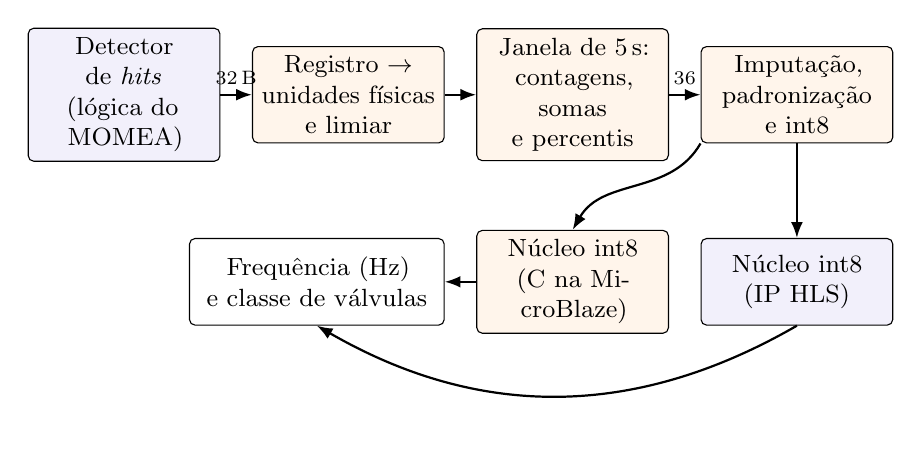
\begin{tikzpicture}[
		font=\small, node distance=4mm and 4mm,
		bloco/.style={draw, rounded corners=2pt, align=center, minimum height=11mm, text width=22mm, fill=white},
		hw/.style={bloco, fill=blue!6},
		sw/.style={bloco, fill=orange!8},
		seta/.style={-{Latex[length=2mm]}, thick}]
		\node[hw] (det) {Detector de \textit{hits}\\(lógica do MOMEA)};
		\node[sw, right=of det] (conv) {Registro \(\to\)\\unidades físicas\\e limiar};
		\node[sw, right=of conv] (jan) {Janela de 5\,s:\\contagens, somas\\e percentis};
		\node[sw, right=of jan] (pre) {Imputação,\\padronização\\e int8};
		\node[hw, below=12mm of pre] (hls) {Núcleo int8\\(IP HLS)};
		\node[sw, left=of hls] (mbn) {Núcleo int8\\(C na MicroBlaze)};
		\node[bloco, left=of mbn, text width=30mm] (out) {Frequência (Hz)\\e classe de válvulas};
		\draw[seta] (det) -- node[above, font=\scriptsize]{32\,B} (conv);
		\draw[seta] (conv) -- (jan);
		\draw[seta] (jan) -- node[above, font=\scriptsize]{36} (pre);
		\draw[seta] (pre) -- (hls);
		\draw[seta] (pre.south west) to[out=-120, in=60] (mbn.north);
		\draw[seta] (mbn) -- (out);
		\draw[seta] (hls.south) to[out=-150, in=-30] (out.south);
	\end{tikzpicture}
	\caption{Cadeia embarcada. Em azul, lógica dedicada; em laranja, \textit{software} na MicroBlaze. O núcleo int8 tem uma única fonte em C, que compila para a MicroBlaze ou é sintetizada como IP pelo Vitis HLS.}
	\label{sim:fig:cadeia}
\end{figure}

\subsection{Implementação}
\label{sim:sec:implementacao}

\paragraph{Conversão e descritores.} O registro traz o pico em códigos (\(|x - z_c|\)), as contagens, o tempo de subida e a duração em amostras e a energia bruta \(\sum u^2\) em 48 bits. Com o fator de calibração do canal \(v_c\) (volts por código) e o ganho \(G = 10^{34/20}\),
\begin{equation}
	V_p = p\, v_c, \qquad
	A = 20 \log_{10}\frac{V_p}{G \cdot 1\,\mu\mathrm{V}}, \qquad
	E = \frac{\sum u^2\, (v_c/G)^2}{f_s \cdot 10^{-14}\,\mathrm{V^2 s}}, \qquad
	t = \frac{n}{f_s},
	\label{sim:eq:conversao}
\end{equation}
com \(E\) em eu e \(f_s = 10\,\)MSa/s; os fatores constantes são calculados uma vez por canal. Cada \textit{hit} atualiza contagens e somas da janela e, se não foi truncado, guarda sete valores para os percentis. No modo \textbf{exato}, esses valores ficam em vetores de até 1\,024 posições por canal, ordenados por \textit{heapsort} ao fechar a janela e interpolados como no \texttt{numpy} \cite{hyndman1996} (65,6\,kB); no modo \textbf{histograma}, cada variável tem um histograma de largura fixa (10,3\,kB e custo constante por \textit{hit}), alternativa para taxas altas de \textit{hits}.

\paragraph{Quantização.} A entrada é padronizada em ponto flutuante, saturada em \(\pm 8\) desvios e quantizada como \(q^x = \mathrm{rint}(z \cdot 127/8)\). Os pesos usam escala simétrica por camada (\(s_W = \max|W|/127\)), e as escalas das ativações foram calibradas no percentil 99,9 do máximo por janela. Cada camada densa com ReLU acumula em 32 bits e requantiza por uma multiplicação inteira e um deslocamento \cite{jacob2018,krishnamoorthi2018}:
\begin{equation}
	\begin{gathered}
		a_o = \sum_{i} q^{x}_{i}\, q^{W}_{io} + q^{b}_{o}, \qquad
		M = \mathrm{round}\!\left(2^{31}\,\frac{s_x\, s_W}{s_y}\right), \\
		q^{y}_{o} = \min\!\left(127,\ \left\lfloor \frac{\max(a_o, 0)\, M + 2^{30}}{2^{31}} \right\rfloor\right),
	\end{gathered}
	\label{sim:eq:requant}
\end{equation}
em que \(s_x\), \(s_W\) e \(s_y\) são as escalas da entrada, dos pesos e da saída. A camada de saída mantém o acumulador de 32 bits, convertido em Hz (regressor) ou usado no \(\arg\max\) (classificador). Como a Equação~\eqref{sim:eq:requant} é determinística, pode-se exigir igualdade bit a bit entre implementações; para isso, a quantização da entrada foi emulada em Python com as mesmas operações em precisão simples e o mesmo arredondamento do C \cite{goldberg1991,ieee754}, e o C foi compilado sem contração em FMA.

\paragraph{Núcleo int8 com fonte única.} As duas redes são escritas como laços de multiplicação e acumulação, com pesos em vetores constantes gerados do modelo treinado. O mesmo arquivo compila com \texttt{gcc} no computador, com \texttt{mb-gcc} para a MicroBlaze e no Vitis HLS como função de topo. No HLS, cada laço interno tem \textit{pipeline} com intervalo de iniciação 1, os pesos viram ROMs e a interface é AXI4-Lite; a escolha privilegia área, pois uma decisão a cada 5\,s não justifica paralelismo.

\subsection{Verificação por simulação}
\label{sim:sec:verificacao}

A verificação foi organizada em seis níveis, cada um com sua referência e seu critério de aceitação (Tabela~\ref{sim:tab:niveis}). Os níveis V1 a V3 usam todos os dados; V4 e V5 usam subconjuntos, porque a simulação RTL é lenta.

\begin{table}[htbp]
	\centering
	\small
	\caption{Níveis de verificação e critérios de aceitação.}
	\label{sim:tab:niveis}
	\begin{tabular}{L{0.06\textwidth}L{0.28\textwidth}L{0.30\textwidth}L{0.26\textwidth}}
		\toprule
		\textbf{Nível} & \textbf{O que se verifica} & \textbf{Como} & \textbf{Critério} \\
		\midrule
		V0 & Exportação do modelo & Rede em ponto flutuante reconstruída a partir dos pesos exportados, contra o \texttt{scikit-learn} & Diferença numérica desprezível; classes iguais \\
		V1 & Inferência em C no PC & 3\,540 janelas; float32 contra Python e int8 contra a emulação inteira & int8 bit a bit; float32 com diferença \(< 10^{-2}\)\,Hz \\
		V2 & Cadeia completa no PC & 281\,595 \textit{hits} \(\to\) descritores em C \(\to\) MLP int8, contra os descritores e as saídas int8 do Python & Erro normalizado \(\le 10^{-3}\); NaN idênticos; mesma classe e nível \\
		V3 & Núcleo HLS & csim e cosim C/RTL (Verilog, xsim) com 256 janelas & Acumuladores e classe idênticos \\
		V4 & Implementação do IP & Síntese e roteamento fora de contexto no XC7A35T, 100\,MHz & Temporização atendida \\
		V5 & Programa na MicroBlaze & Simulação RTL do processador executando o ELF final; até 2 janelas reais (163 \textit{hits}) e 2 vetores para a MLP & Resultados idênticos aos do PC; ciclos medidos \\
		\bottomrule
	\end{tabular}
\end{table}

O nível V5 substitui a medição em placa. Um sistema mínimo foi montado no Vivado 2022.2 para a mesma peça do MOMEA (xc7a35ticsg324-1L): MicroBlaze v11 com \textit{pipeline} de cinco estágios, sem caches, com \textit{barrel shifter}, multiplicador e divisor, 128\,kB de memória local em BRAM e um GPIO de 32 bits; foram simuladas as configurações sem FPU e com FPU estendida \cite{amd_ug984}. O programa escreve uma marca no GPIO antes e depois de cada etapa (processar os \textit{hits}, fechar a janela, executar a MLP), e o testbench registra o ciclo de cada mudança; ao fim de cada janela, escreve também a classe e parte do acumulador, e a sequência simulada tem de ser idêntica à do computador \cite{amd_ug900}. Como a memória é local e não há interrupções nem pilha de rede, os ciclos medidos são o melhor caso do código; no \textit{firmware} real, o tempo de parede será maior.


% -------------------------------------------------------------------------------------------------------
\section{Validação externa na base CWRU}
\label{sec:mm_cwru}
% Gerado por ferramentas/importar_relatorios.py a partir de CWRU/RELATORIO_CWRU-10.11.2026/RELATORIO_CWRU.tex.
% Revisado à mão na dissertação: edite este arquivo, não a fonte.
\subsection{Objetivo e enquadramento}
\label{cwru:sec:objetivo}

O estudo da bomba (Seção~\ref{sec:mm_bomba}) mostrou que modelos treinados com descritores de \textit{hits} reconhecem bem as condições quando a corrida aparece no treino, mas generalizam mal quando a corrida inteira é deixada de fora, e que os dados tinham problemas de aquisição: 70\,\% dos \textit{hits} saturados e muitos truncados pela duração máxima. Como os dados do ensaio têm uma única corrida por condição, não era possível separar o que é limitação do método do que é limitação dos dados.

A base CWRU \cite{cwru} é a referência mais usada em diagnóstico de rolamentos e permite testar o mesmo fluxo em dados públicos e rotulados. Ela tem, porém, uma estrutura parecida com a do ensaio da bomba: cada rolamento com defeito foi montado uma vez e gravado em quatro cargas, de modo que há poucas unidades físicas independentes. Parte da literatura relata acurácias próximas de 100\,\% com janelas sorteadas, e trabalhos posteriores mostraram que esses números caem quando a divisão respeita as gravações ou os rolamentos \cite{smith2015,rauber2021,hendriks2022}.

Os sinais são de vibração (acelerômetros a 48\,kHz), e não de EA. O extrator de \textit{hits} do MOMEA é aplicado aqui como detector de impulsos: os defeitos localizados produzem impactos periódicos, e a lógica de limiar, DDT e rearme se aplica a eles. Os descritores, porém, têm outro significado físico, e as conclusões sobre cavitação não se transferem. O objetivo é responder a três perguntas:
\begin{enumerate}
	\item os descritores de \textit{hits} no estilo MOMEA capturam a física do defeito?
	\item como a acurácia depende da validação, quando as unidades físicas são separadas?
	\item o fluxo embarcado (MLP int8) preserva a decisão?
\end{enumerate}

% =======================================================================================================

% Gerado por ferramentas/importar_relatorios.py a partir de CWRU/RELATORIO_CWRU-10.11.2026/RELATORIO_CWRU.tex.
% Revisado à mão na dissertação (versão enxuta): edite este arquivo, não a fonte.
\subsection{Base de dados}
\label{cwru:sec:dados}

Foram usados os sinais do acelerômetro do lado do acionamento (DE), a 48\,kHz, dos conjuntos \textit{48k Drive End Bearing Fault Data} e \textit{Normal Baseline Data} \cite{cwru}. O rolamento é um 6205-2RS JEM SKF, com frequências de defeito de 5,4152 (pista interna, BPFI), 3,5848 (pista externa, BPFO) e 2,3570 (esfera, BSF) vezes a frequência de rotação. O subconjunto tem delineamento cruzado completo: máquina sã (N) e defeitos por eletroerosão na pista interna (IR), na esfera (B) e na pista externa na zona de carga (OR@6h), com diâmetros de 0,007, 0,014 e 0,021~polegada, nas cargas de 0 a 3\,HP. São 40 gravações de cerca de 10\,s. As inconsistências conhecidas dos arquivos foram tratadas explicitamente: arquivos com variáveis de outras gravações (usou-se sempre a de número igual ao do arquivo), um arquivo com apenas 1,3\,s, uma rotação ausente (usou-se a nominal) e cinco gravações com saturação em \(\pm 3{,}418\,g\), em fração desprezível. Cada gravação foi dividida em janelas de 0,25\,s (cerca de 7 rotações), sem sobreposição, num total de 1\,376 janelas: 140 da máquina sã, 396 de IR, 420 de B e 420 de OR.

\subsection{Métodos}
\label{cwru:sec:metodos}

O extrator reproduz a lógica do MOMEA sobre \(|x - \bar{x}|\) (início no primeiro cruzamento, término após o DDT, HLT re-armável com ROVL e truncamento por MAXDUR), com os tempos escalados para 48\,kHz: DDT e HLT de 1\,ms e duração máxima de 20\,ms. Foram comparados dois limiares: \textbf{fixo}, de 0,3\,\(g\), como o MOMEA opera hoje; e \textbf{flutuante}, de 1,5 vez o RMS da janela anterior (causal), com mínimo de 0,3\,\(g\), análogo ao de sistemas comerciais de EA \cite{vallen2022} e implementável na lógica. O fator 1,5 e o DDT foram escolhidos por varredura, pelo critério de a ordem do intervalo entre \textit{hits} coincidir com BPFO e BPFI; o critério usa os rótulos, mas não a divisão de treino e teste de nenhuma validação.

Três grupos de descritores foram calculados por janela:
\begin{itemize}
	\item \textbf{clássicos} (8): RMS, pico, fator de crista, curtose, assimetria e fatores de forma, de impulso e de folga;
	\item \textbf{envelope} (7): curtose do envelope e amplitudes do espectro do envelope (filtro de 1 a 10\,kHz) em 1\(\times\) e 2\(\times\) BPFO, BPFI e 2\(\times\)BSF, em dB acima da mediana \cite{randall2011};
	\item \textbf{\textit{hits}} (14): taxa, frações truncadas e com ROVL, percentis dos descritores e, como medidas de periodicidade, a ordem do intervalo entre \textit{hits}, \((1/\mathrm{mediana}\,\Delta t)/f_r\), e seu coeficiente de variação.
\end{itemize}

A MLP tem os hiperparâmetros do estudo da bomba \cite{pedregosa2011}, e uma \textit{Random Forest} serve de referência. As tarefas são quatro classes (N, IR, B, OR) e dez classes (tipo e diâmetro), com três validações de independência crescente: \textbf{janelas sorteadas} (5 partes estratificadas); \textbf{carga deixada de fora} (LOLO, 4 partes), que separa gravações, mas não rolamentos; e \textbf{diâmetro deixado de fora} (LOSO, 3 partes, só em quatro classes), em que o teste contém rolamentos físicos nunca vistos, análogo ao LORO da bomba. As métricas são a acurácia por janela e por gravação (voto majoritário).


% -------------------------------------------------------------------------------------------------------
\section{Ferramentas e ambiente de desenvolvimento}
\label{sec:mm_ferramentas}

O \textit{hardware} do extrator usa a placa Arty A7-35T, com o FPGA Artix-7 XC7A35T \cite{xilinx2020ds180}. O desenvolvimento usou o ecossistema da AMD/Xilinx, versão 2022.2:
\begin{itemize}
	\item \textbf{Vivado Design Suite}: síntese, implementação, integração de blocos (\textit{IP Integrator}) e simulação lógica (\textit{Vivado Simulator}, xsim). As métricas de utilização de recursos (LUTs, \textit{flip-flops}, BRAMs e DSPs) e de temporização foram obtidas dessa ferramenta \cite{amd_ug900};
	\item \textbf{Vitis HLS}: síntese de alto nível do núcleo da MLP a partir de C, com simulação C, cossimulação C/RTL e exportação como IP. Diretivas como \textit{pipeline} e desenrolamento de laços controlam o compromisso entre latência e área \cite{amd_ug1399,cong2011hls};
	\item \textbf{Vitis} e \texttt{mb-gcc}: compilação do \textit{firmware} e dos programas da MicroBlaze \cite{amd_ug984};
	\item \textbf{Python 3}, com \texttt{numpy}, \texttt{pandas}, \texttt{scipy}, \texttt{matplotlib} e \texttt{scikit-learn} \cite{pedregosa2011}: análise dos registros, treinamento e validação dos modelos, exportação dos pesos e geração das figuras.
\end{itemize}
Os \textit{scripts} de cada etapa estão organizados nos repositórios do projeto e permitem reproduzir os resultados do Capítulo~\ref{chap:resultados} a partir dos dados brutos.


\chapter{Resultados e Discussão}
\label{chap:resultados}
% =======================================================================================================
% Capítulo 4 - Resultados e Discussão
% =======================================================================================================

Este capítulo apresenta os resultados na mesma ordem do Capítulo~\ref{chap:metodos}: o ensaio do extrator de \textit{hits} contra o sistema comercial (Seção~\ref{sec:res_extrator}), a classificação das condições da bomba a partir dos registros (Seção~\ref{sec:res_bomba}), a implementação embarcada da classificação (Seção~\ref{sec:res_embarcado}) e a validação externa na base CWRU (Seção~\ref{sec:res_cwru}). A Seção~\ref{sec:discussao_integrada} reúne os resultados para responder às questões que motivaram o trabalho.

% -------------------------------------------------------------------------------------------------------
\section{Extrator de \textit{hits}: ensaio simultâneo com o AMSY-6}
\label{sec:res_extrator}
% Gerado por ferramentas/importar_relatorios.py a partir de ARTIGO_V2-10.11.2026/6-Resultados_discussao2.tex.
% Revisado à mão na dissertação: edite este arquivo, não a fonte.
% =======================================================================================================

Esta seção apresenta os resultados dos ensaios descritos na Seção~\ref{sec:mm_delineamento}. Ela reúne os resultados preliminares obtidos até o momento e o plano de análise para as condições ainda não ensaiadas.

Nenhum resultado esperado é incorporado antecipadamente à redação. Em particular, não se pressupõe convergência para 100\% de detecção em amplitudes elevadas, superioridade de um dos sistemas próximo ao limiar, subestimação obrigatória das contagens ou adequação ao Projeto MOMEA. Essas hipóteses podem orientar a investigação, mas as conclusões decorrem dos dados, das incertezas e dos critérios de aceitação previamente definidos.

Os resultados apresentados são os da sessão simultânea R1 (15/10/2026: bursts senoidais de 10 ciclos a 50, 200 e 450\,kHz, \(\approx 95\,\mathrm{dB}_{\mathrm{AE}}\), pré-amplificadores de 34\,dB, blocos de 1 a 10\,000 \textit{bursts} em 30\,s). Eles são identificados como preliminares porque ainda faltam as repetições independentes da sessão, a referência elétrica medida no osciloscópio e a varredura de amplitude e SNR. Nas partes ainda sem dados, o texto descreve o plano de análise.

A apresentação distingue:
\begin{enumerate}
	\item Desempenho de detecção e de segmentação;
	
	\item Erro dos descritores em relação à referência elétrica independente;
	
	\item Concordância entre o sistema proposto e o AMSY-6;
	
	\item Influência do plano de injeção e das configurações instrumentais; e
	
	\item Desempenho computacional, integridade da comunicação e redução do volume de dados.
\end{enumerate}

% -------------------------------------------------------------------------------------------------------
\subsection{Integridade dos dados e população analisada}
\label{v2:subsec:integridade_resultados}

Antes de qualquer comparação paramétrica, é apresentada a rastreabilidade dos estímulos e registros. Para o sistema proposto, os contadores documentam, quando disponíveis:
\begin{equation}
	N_{\mathrm{ger}} \longrightarrow N_{\mathrm{FSM}} \longrightarrow N_{\mathrm{DMA}} \longrightarrow N_{\mathrm{tx}} \longrightarrow N_{\mathrm{rx}}
	\label{v2:eq:fluxo_contadores_resultados}
\end{equation}

\noindent
em que \(N_{\mathrm{ger}}\) é o número de estímulos aplicados, \(N_{\mathrm{FSM}}\) é o número de registros consolidados pela lógica, \(N_{\mathrm{DMA}}\) é o número entregue ao caminho de memória, \(N_{\mathrm{tx}}\) é o número transmitido e \(N_{\mathrm{rx}}\) é o número recebido e validado pelo computador hospedeiro.

As diferenças entre contadores consecutivos são apresentadas separadamente. A condição \(N_{\mathrm{rx}}<N_{\mathrm{FSM}}\), por exemplo, não demonstra falha de detecção; ela indica perda posterior à máquina de estados. Para o AMSY-6, são preservados e reportados os indicadores de saturação, \textit{timeout}, enchimento de \textit{buffer}, modo de longa duração e demais estados relevantes disponibilizados pelo sistema \cite{vallen2022}. Para cada condição experimental, são informados:

\begin{itemize}
	\item Número de estímulos programados e confirmados pela forma de onda de referência;
	
	\item Número de \textit{hits} produzidos por cada sistema;
	
	\item Número de estímulos sem registro associado;
	
	\item Número de associações unívocas, fragmentações e fusões;
	
	\item Número de falsos \textit{hits} nos intervalos contendo apenas ruído;
	
	\item Número de registros saturados, encerrados por \textit{timeout}, com transbordo ou com outro indicador de exceção;
	
	\item Número de perdas, duplicações e registros fora de ordem em cada camada observável; e
	
	\item Número e motivo das exclusões realizadas antes de cada análise.
\end{itemize}

\textbf{Resultados preliminares (R1).} A Tabela~\ref{v2:tab:fluxo_r1} resume a seleção dos registros na sessão R1, com as três frequências somadas. Na versão ensaiada, \(N_{\mathrm{FSM}}\) corresponde ao \texttt{HITCNT}, \(N_{\mathrm{DMA}}\) e \(N_{\mathrm{tx}}\) aos contadores do \textit{firmware} e \(N_{\mathrm{rx}}\) ao total gravado; não houve diferença entre \(N_{\mathrm{FSM}}\) e \(N_{\mathrm{rx}}\).

\begin{table}[htbp]
	\centering
	\footnotesize
		\caption{Seleção dos estímulos e registros na sessão R1 (15/10/2026), três frequências somadas (preliminar).}
	\label{v2:tab:fluxo_r1}
	\begin{tabular}{|p{0.30\textwidth}|p{0.30\textwidth}|p{0.30\textwidth}|}
		\hline
		\textbf{Etapa} & \textbf{Sistema proposto} & \textbf{AMSY-6} \\
		\hline
		Estímulos programados & \multicolumn{2}{c|}{\(3 \times 16\,101 = 48\,303\) \textit{bursts}} \\
		\hline
		Registros recebidos & 48\,282 & 47\,009 \\
		\hline
		Excluídos fora dos blocos & 2 (desligamento das saídas do gerador no fim das capturas de 200 e 450\,kHz) & 3 (transitório de configuração do gerador no início de cada captura) \\
		\hline
		Registros de \textit{bursts} & 48\,280 & 47\,006 \\
		\hline
		Estímulos sem registro próprio & 23, todos explicados no detector: 20 absorvidos no rearme (\textit{hits} com ROVL) e 3 em 2 \textit{hits} fundidos & 1\,297; 1\,086 \textit{hits} com indicador R \\
		\hline
		Exclusões por SAT ou MAXDUR & 0 & --- \\
		\hline
		Perdas na comunicação & 0/48\,280 & --- \\
		\hline
	\end{tabular}
\end{table}


As regras de exclusão são definidas antes da inspeção dos resultados e aplicadas de maneira simétrica. Registros saturados ou fragmentados não são simplesmente descartados: sua frequência é um resultado do experimento. Eles podem ser excluídos de uma análise específica de linearidade ou concordância, desde que permaneçam contabilizados e sejam apresentados em estrato próprio. Regra proposta, a fixar antes da análise final: registros com SAT, MAXDUR ou acumulador saturado entram nas contagens de detecção e formam estrato próprio; ficam fora das análises de linearidade e de concordância dos descritores; e o número de cada caso é reportado. \textit{Hits} fundidos (contagens múltiplas do esperado) entram na análise de detecção como fusão. Nos ensaios até 15/10/2026, não ocorreu nenhum \textit{hit} com SAT ou MAXDUR.

% -------------------------------------------------------------------------------------------------------
\subsection{Desempenho de detecção e segmentação}
\label{v2:subsec:concordancia_deteccao_resultados}

A análise de detecção segue a regra de associação da Subseção~\ref{v2:subsec:metricas_comparacao}. Para cada sistema e condição, são apresentadas:
\begin{itemize}
	\item Proporção de estímulos com ao menos um \textit{hit} associado;
	
	\item Proporção de associações unívocas \(1{:}1\);
	
	\item Proporções de ausência de detecção, fragmentação e fusão;
	
	\item Taxa de falsos \textit{hits} por unidade de tempo de fundo; e
	
	\item Intervalos de confiança compatíveis com o delineamento em blocos.
\end{itemize}

Para expressar a amplitude em relação ao limiar em uma base comum, define-se:
\begin{equation}
	\rho_i = \frac{V_{\mathrm{pico,ref},i}}{V_{\mathrm{th,ref}}}, \qquad A_{\mathrm{exc},i} = 20\log_{10}\left(\rho_i\right)
	\label{v2:eq:amplitude_relativa_limiar_resultados}
\end{equation}

\noindent
em que \(V_{\mathrm{pico,ref},i}\) é a amplitude do estímulo medida no plano de referência e \(V_{\mathrm{th,ref}}\) é o limiar referido ao mesmo plano. Essa normalização é válida somente quando as conversões de ganho e limiar estão calibradas e quando a grandeza utilizada pelo comparador é compatível. Se os sistemas operarem sobre sinais de decisão distintos, os valores em volts e as configurações originais também são apresentados.

A probabilidade de detecção é representada em função de \(A_{\mathrm{exc}}\), ou da SNR, separadamente para frequências, durações e demais fatores capazes de alterar a resposta. A agregação de condições heterogêneas em uma única curva pode produzir uma transição artificialmente larga ou deslocada.

Quando a faixa de amplitudes contiver observações abaixo e acima da região de transição e o ajuste for adequado, pode-se utilizar um modelo binomial. Em sua forma mais simples, para o sistema \(j\),
\begin{equation}
	\operatorname{logit} \left[p_j\left(A_{\mathrm{exc}}\right) \right] = \beta_{0,j} + \beta_{1,j}A_{\mathrm{exc}}	\label{v2:eq:modelo_deteccao_logistico}
\end{equation}

\noindent
com:
\begin{equation}
	\operatorname{logit}(p) = \ln \left(\frac{p}{1-p}\right)
\end{equation}

Se houver agrupamento por aquisição ou bloco, emprega-se um modelo binomial de efeitos mistos ou outra abordagem que preserve essa dependência. Frequência, SNR, duração e sistema podem ser incluídos como fatores, com interações justificadas pelo delineamento. 

A amplitude relativa associada a uma probabilidade \(q\) é estimada por:
\begin{equation}
	A_{q,j} = \frac{\operatorname{logit}(q)-\widehat{\beta}_{0,j}}{\widehat{\beta}_{1,j}}
	\label{v2:eq:amplitude_probabilidade_deteccao}
\end{equation}

Podem ser reportados \(A_{50}\) e \(A_{90}\), acompanhados de intervalos de confiança. Esses valores não são extrapolados quando a matriz não abrange a probabilidade correspondente, quando a curva não é aproximadamente monotônica ou quando há separação completa sem informação suficiente para estimar a transição.

A afirmação de que diferenças próximas ao limiar decorrem exclusivamente da diferença nominal entre 12 e 16 bits é insuficiente. A interpretação considera ruído referido à entrada, ENOB, faixa de entrada, ganho, resposta dos filtros, quantização do limiar e convenção do sinal de decisão.

\textbf{Resultados preliminares (R1).} A Tabela~\ref{v2:tab:deteccao_r1} resume a detecção por frequência e a Tabela~\ref{v2:tab:carga_r1}, por bloco de carga. Como a associação foi feita por bloco (sem \textit{timestamp}), \(N_{1:1}\) é estimado como os registros com 10 contagens e sem ROVL. O sistema proposto detectou de 99,94 a 99,96\,\% dos \textit{bursts} por frequência, e o AMSY-6, de 96,8 a 97,6\,\%. Não houve fragmentação: todos os \textit{hits} do sistema proposto têm 10 contagens ou múltiplos de 10. Houve 2 fusões no sistema proposto em 50\,kHz, cobrindo 3 \textit{bursts} extras. Nos blocos de 1, 100 e 1000 \textit{bursts} (intervalos \(\ge 30\,\mathrm{ms}\)), nenhum dos sistemas deixou de registrar estímulos; as diferenças concentram-se nos blocos de 5000 e 10\,000, em que o intervalo entre estímulos (6 e 3\,ms) se aproxima do tempo de ocupação do canal (duração + DDT + RAT \(\approx 2{,}3\)--\(2{,}4\,\mathrm{ms}\)).

\begin{table}[htbp]
	\centering
	\footnotesize
		\caption{Detecção por frequência na sessão R1 (16\,101 \textit{bursts} por frequência; preliminar).}
	\label{v2:tab:deteccao_r1}
	\begin{tabular}{|c|c|c|c|c|c|c|}
		\hline
		 & \multicolumn{4}{c|}{\textbf{Sistema proposto}} & \multicolumn{2}{c|}{\textbf{AMSY-6}} \\
		\cline{2-7}
		\textbf{Freq.} & \textbf{Registrados} & \textbf{Detecção} & \textbf{ROVL} & \textbf{Fundidos} & \textbf{Registrados} & \textbf{Detecção} \\
		\hline
		50\,kHz & 16\,094 & 99,96\,\% & 4 & 2 & 15\,580 & 96,8\,\% \\
		\hline
		200\,kHz & 16\,092 & 99,94\,\% & 9 & 0 & 15\,716 & 97,6\,\% \\
		\hline
		450\,kHz & 16\,094 & 99,96\,\% & 7 & 0 & 15\,710 & 97,6\,\% \\
		\hline
	\end{tabular}
\end{table}

\begin{table}[htbp]
	\centering
	\footnotesize
		\caption{Registros por bloco de carga na sessão R1 (diferença em relação ao número de \textit{bursts} entre parênteses; preliminar).}
	\label{v2:tab:carga_r1}
	\setlength{\tabcolsep}{3pt}
	\begin{tabular}{|p{0.13\textwidth}|c|c|c|c|c|c|}
		\hline
		\textbf{Bloco (30\,s)} & \textbf{50\,kHz P} & \textbf{50\,kHz A} & \textbf{200\,kHz P} & \textbf{200\,kHz A} & \textbf{450\,kHz P} & \textbf{450\,kHz A} \\
		\hline
		1, 100 e 1000 & sem perda & sem perda & sem perda & sem perda & sem perda & sem perda \\
		\hline
		5000 (6\,ms) & 5000 (0) & 4983 (\(-17\)) & 4997 (\(-3\)) & 4975 (\(-25\)) & 4999 (\(-1\)) & 4985 (\(-15\)) \\
		\hline
		10\,000 (3\,ms) & 9993 (\(-7\)) & 9496 (\(-504\)) & 9994 (\(-6\)) & 9640 (\(-360\)) & 9994 (\(-6\)) & 9624 (\(-376\)) \\
		\hline
		\multicolumn{7}{|l|}{P: sistema proposto; A: AMSY-6.} \\
		\hline
	\end{tabular}
\end{table}


% -------------------------------------------------------------------------------------------------------
\subsection{Concordância e diferenças paramétricas}
\label{v2:subsec:concordancia_parametrica_resultados}

A análise paramétrica principal utiliza estímulos com associação unívoca nos dois sistemas. Os casos de saturação, \textit{timeout}, fragmentação, fusão e transbordo são apresentados separadamente. Para cada descritor, apresentam-se:

\begin{itemize}
	\item Distribuição dos valores de referência e dos valores produzidos pelos dois sistemas;
	
	\item Gráfico do sistema proposto em função do AMSY-6, com linha de identidade e escalas iguais;
	
	\item Gráfico de Bland--Altman das diferenças em função da magnitude;
	
	\item Viés, desvio-padrão das diferenças, limites de concordância e intervalos de confiança; e
	
	\item Resultados estratificados pelos fatores para os quais houver evidência de alteração do viés ou da dispersão.
\end{itemize}

O procedimento original de Bland--Altman é descrito em \cite{bland1986}. Como existem repetições por condição e por bloco, os limites de concordância consideram medidas repetidas ou são estimados em estratos homogêneos. A extensão metodológica para medidas repetidas é apresentada em \cite{bland1999}. Os estratos são as condições experimentais (frequência \(\times\) bloco de carga \(\times\) plano de injeção), e os limites são calculados por condição, ou por modelo de medidas repetidas com a sessão como bloco, com intervalos de confiança, somente para os descritores classificados como equivalentes ou assemelhados no Quadro~\ref{v2:qua:configuracao_pareada_secao5}; para contagens, reporta-se a distribuição das discordâncias. A simples aplicação de \(\overline{d}\pm1{,}96s_d\) a todos os pulsos, ignorando o agrupamento, pode subestimar a incerteza. O coeficiente de correlação, quando apresentado, permanece suplementar e não pode fundamentar afirmações de concordância.

O Quadro~\ref{v2:qua:interpretacao_descritores_secao6} organiza as verificações necessárias. As possíveis origens listadas não constituem diagnósticos automáticos; uma divergência pode resultar de mais de um mecanismo. Segundo a especificação do fabricante, o processamento convencional dos \textit{hits} no AMSY-6 opera a \(10\,\mathrm{MHz}\) \cite{vallen2022}.

\begingroup
\renewcommand{\tablename}{Quadro}
\footnotesize
\renewcommand{\arraystretch}{1.22}
\begin{longtable}{|
		>{\raggedright\arraybackslash}p{2.5cm}|
		>{\raggedright\arraybackslash}p{4.0cm}|
		>{\raggedright\arraybackslash}p{4.1cm}|
		>{\raggedright\arraybackslash}p{3.6cm}|}
	\caption{Análises e cuidados de interpretação para os descritores.}
	\label{v2:qua:interpretacao_descritores_secao6}\\
	\hline
	\textbf{Descritor} & \textbf{Apresentação mínima} & \textbf{Fontes plausíveis de diferença} & \textbf{Verificação necessária} \\
	\hline
	\endfirsthead
	\multicolumn{4}{c}
	{\tablename\ \thetable{} -- continuação}\\
	\hline
	\textbf{Descritor} & \textbf{Apresentação mínima} & \textbf{Fontes plausíveis de diferença} & \textbf{Verificação necessária} \\
	\hline
	\endhead
	\hline
	\multicolumn{4}{r}{Continua na próxima página.}\\
	\endfoot
	\hline
	\endlastfoot
	Amplitude & Volts no plano comum, \(\mathrm{dB}_{\mathrm{AE}}\), erro perante a referência, dispersão, Bland--Altman e linearidade. & Ganho calibrado, resposta em frequência, carregamento, faixa de entrada, fase de amostragem, quantização, não linearidade e saturação. & Calibração da cadeia completa e ensaios em frequência e amplitude. \\
	\hline
	Tempo de subida & Erro em tempo e em unidades da grade de processamento; diferenças em função de frequência, amplitude e duração. & Limiar, resposta transitória e fase dos filtros, instante do pico, amostragem, interpolação e definição da primeira ocorrência do pico. & Comparar formas de onda de referência e respostas impulsivas ou de grupo das cadeias. \\
	\hline
	Duração & Diferença em tempo e amostras, distribuição discreta e estratificação por DDT. & Primeiro e último cruzamentos, sinal de decisão, limiar, filtragem, quantização temporal e convenção de encerramento. & Confirmar que a duração termina no último cruzamento e não na expiração do DDT. \\
	\hline
	Contagens & Diferença inteira, distribuição das discordâncias e análise por frequência, amplitude e SNR. & Filtragem, limiar, sinal com sinal ou módulo, grade de processamento, histerese, DDT, fase relativa e ruído. & Não atribuir a diferença diretamente a \(8\) contra \(40\,\mathrm{MS/s}\); comparar as grades efetivamente utilizadas na extração dos descritores. \\
	\hline
	Energia & \(\mathrm{V^2s}\), eu, razão ou diferença em escala logarítmica, erro perante a referência e indicação de saturação. & Fator de escala, janela integrada, ruído, filtros, truncamento, saturação, largura do acumulador e arredondamento. & Comparar \textit{True Energy} com a integral quadrática definida na Subseção~\ref{v2:subsec:energia_ea}; tratar \textit{Signal Strength} separadamente. \\
	\hline
	Tempo de chegada & Diferença temporal, deslocamento inicial e deriva ao longo de cada aquisição. & Bases de tempo, sincronização, atraso dos filtros, limiar e regra de interpolação. & Medir ou estimar deslocamento e deriva; não interpretar tempo absoluto sem sincronização. \\
\end{longtable}
\endgroup

Se a diferença for proporcional à magnitude, a análise em escala logarítmica é mais apropriada, desde que os valores sejam positivos. Nesse caso, são reportadas razões geométricas e limites multiplicativos, e não uma mistura entre diferenças em escala original e logarítmica.

% -------------------------------------------------------------------------------------------------------
\subsection{Erro em relação à referência elétrica independente}
\label{v2:subsec:exatidao_referencia_resultados}

Esta análise compara os dois instrumentos com os descritores obtidos da forma de onda elétrica medida independentemente, conforme a hierarquia da Subseção~\ref{v2:subsec:sistema_referencia_experimento}. A referência possui incerteza e depende do plano de medição, da banda e do processamento \textit{off-line}.

Os parâmetros nominais dos estímulos (Subseção~\ref{v2:subsec:sinais_teste}) fornecem diretamente pico e energia do sinal ideal, mas não fornecem automaticamente todos os descritores observados após filtros, ruído, amostragem, limiar e DDT. Tempo de chegada, tempo de subida, duração e contagens são calculados sobre a forma de onda de referência efetivamente medida, empregando as definições da Seção~\ref{sec:fund_hits}.

Para cada descritor e instrumento, são apresentados os erros definidos na Seção~\ref{sec:mm_delineamento}, acompanhados de viés, MAE, RMSE e intervalos de confiança. A incerteza-padrão combinada da diferença pode ser representada, em uma forma geral, por:

\begin{equation}
	u_{\mathrm{c}}^2\left(e_x\right) = u^2\left(x^{(j)}\right) + u^2\left(x_{\mathrm{ref}}\right) - 2\operatorname{cov} \left(	x^{(j)}, x_{\mathrm{ref}}\right)
	\label{v2:eq:incerteza_erro_referencia}
\end{equation}

\noindent
em que a covariância é mantida quando o descritor do instrumento e o de referência compartilham fatores de calibração ou dados. O orçamento de incerteza é compatível com o modelo definido conforme o JCGM~100 \cite{jcgm2008}.

Uma conclusão de equivalência é defensável somente se os intervalos obtidos forem confrontados com tolerâncias previamente estabelecidas. Ser mais próximo da referência do que o outro instrumento não demonstra, por si só, adequação à aplicação.

\textbf{Resultados preliminares (R1).} Ainda não há descritores de referência: falta capturar no osciloscópio a forma de onda efetivamente injetada. A comparação entre os instrumentos na sessão R1, com a amplitude do sistema proposto recalculada para o ganho de 34\,dB, está na Tabela~\ref{v2:tab:descritores_r1}, e os valores por bloco, na Tabela~\ref{v2:tab:valores_bloco_r1}. Nesse ensaio, o \textit{software} de aquisição do sistema proposto estava configurado com ganho de 35\,dB, de modo que o limiar efetivo foi de \(81\,\mathrm{dB}_{\mathrm{AE}}\).

\begin{table}[htbp]
	\centering
	\footnotesize
		\caption{Descritores na sessão R1: sistema proposto \(\times\) AMSY-6 (preliminar).}
	\label{v2:tab:descritores_r1}
	\begin{tabular}{|p{0.22\textwidth}|p{0.20\textwidth}|p{0.20\textwidth}|p{0.20\textwidth}|}
		\hline
		\textbf{Descritor} & \textbf{50\,kHz} & \textbf{200\,kHz} & \textbf{450\,kHz} \\
		\hline
		Amplitude (\(\mathrm{dB}_{\mathrm{AE}}\)) & 95,78 \(\times\) 95,30 (\(+0{,}47\)\,dB) & 95,79 \(\times\) 95,04 (\(+0{,}76\)\,dB) & 95,88 \(\times\) 95,29 (\(+0{,}59\)\,dB) \\
		\hline
		Desvio-padrão da amplitude & 0,06 \(\times\) 0,05\,dB & 0,05 \(\times\) 0,06\,dB & 0,04 \(\times\) 0,07\,dB \\
		\hline
		Duração (\(\mu\)s) & 188,8 \(\times\) 226,4 & 47,19 \(\times\) 51,48 & 20,97 \(\times\) 22,84 \\
		\hline
		Duração (períodos) & 9,44 \(\times\) 11,32 & 9,44 \(\times\) 10,30 & 9,44 \(\times\) 10,28 \\
		\hline
		Contagens & 10 \(\times\) 11 (12 em 1,6\,\%) & 10 \(\times\) 11 & 10 \(\times\) 11 \\
		\hline
		Energia (razão proposto/AMSY-6) & 1,28 & 1,36 & 1,44 \\
		\hline
		Energia / (\(A^2/2 \cdot\) duração) & 0,95 \(\times\) 0,69 & 0,97 \(\times\) 0,78 & 0,98 \(\times\) 0,71 \\
		\hline
		Tempo de subida (\(\mu\)s) & \(87 \pm 58\) \(\times\) \(37{,}0 \pm 4{,}7\) & \(27 \pm 15\) \(\times\) \(5{,}34 \pm 0{,}05\) & \(10{,}2 \pm 6{,}5\) \(\times\) \(1{,}45 \pm 0{,}05\) \\
		\hline
	\end{tabular}
\end{table}

A diferença de amplitude, de \(+0{,}47\) a \(+0{,}76\,\mathrm{dB}\), soma a assimetria do divisor e a diferença de ganho entre os pré-amplificadores (34,00 e 34,22\,dB) e só poderá ser separada com o Experimento A. A dispersão da amplitude é pequena e semelhante nos dois sistemas (0,04 a 0,07\,dB). A duração do sistema proposto corresponde a 9,44 períodos em todas as frequências, coerente com a convenção de término no último cruzamento; a do AMSY-6 é maior e varia com a frequência, assim como a contagem de 11 (e 12 em 1,6\,\% dos \textit{hits} em 50\,kHz), o que é compatível com a contagem da oscilação após o fim do \textit{burst}. A energia do sistema proposto é coerente com sua amplitude e duração (razão de 0,95 a 0,98 em relação a \(A^2/2 \cdot t_{\mathrm{dur}}\)); a do AMSY-6 fica 22 a 31\,\% abaixo do que sua própria amplitude e duração indicam. Por isso, duração e energia são tratadas como descritores assemelhados, e não como erros de detecção. O tempo de subida do sistema proposto não é repetível com envelope retangular, porque os 10 ciclos têm o mesmo pico a menos do ruído; a comparação desse descritor exige envelope realista.

\begingroup
\scriptsize
\setlength{\tabcolsep}{2pt}
\renewcommand{\arraystretch}{1.12}
\begin{longtable}{|c|r|c|c|c|c|}
	\caption{Valores por bloco na sessão R1: média [mínimo--máximo] (amplitude do sistema proposto recalculada para 34\,dB; preliminar).}
	\label{v2:tab:valores_bloco_r1}\\
	\hline
	\textbf{Freq.} & \textbf{Bursts} & \textbf{Ampl. P (\(\mathrm{dB}_{\mathrm{AE}}\))} & \textbf{Ampl. A (\(\mathrm{dB}_{\mathrm{AE}}\))} & \textbf{Dur. P (\(\mu\)s)} & \textbf{Dur. A (\(\mu\)s)} \\
	\hline
	\endfirsthead
	\hline
	\textbf{Freq.} & \textbf{Bursts} & \textbf{Amplitude P} & \textbf{Amplitude A} & \textbf{Duração P} & \textbf{Duração A} \\
	\hline
	\endhead
	\hline
	\multicolumn{6}{|l|}{P: sistema proposto; A: AMSY-6.} \\
	\hline
	\endlastfoot
	50\,kHz & 1 & 95,77 [95,77--95,77] & 95,40 [95,4--95,4] & 188,70 [188,7--188,7] & 226,8 [226,8--226,8] \\
	50\,kHz & 100 & 95,76 [95,63--95,90] & 95,31 [95,2--95,4] & 188,76 [188,6--188,9] & 226,5 [225,1--229,7] \\
	50\,kHz & 1000 & 95,76 [95,60--95,93] & 95,30 [95,1--95,5] & 188,76 [188,6--188,9] & 226,4 [214,4--230,4] \\
	50\,kHz & 5000 & 95,78 [95,58--96,03] & 95,30 [95,1--95,5] & 188,76 [188,6--188,9] & 226,4 [214,2--230,9] \\
	50\,kHz & 10\,000 & 95,78 [95,60--96,03] & 95,30 [95,1--95,5] & 188,76 [188,6--188,9] & 226,4 [214,3--230,8] \\
	\hline
	200\,kHz & 1 & 95,79 [95,79--95,79] & 95,10 [95,1--95,1] & 47,20 [47,2--47,2] & 51,4 [51,4--51,4] \\
	200\,kHz & 100 & 95,78 [95,69--95,88] & 95,04 [94,9--95,2] & 47,19 [47,1--47,2] & 51,5 [51,4--51,6] \\
	200\,kHz & 1000 & 95,79 [95,68--96,07] & 95,04 [94,9--95,3] & 47,19 [47,1--47,3] & 51,5 [51,4--51,6] \\
	200\,kHz & 5000 & 95,80 [95,66--96,00] & 95,04 [94,8--95,3] & 47,18 [47,1--47,3] & 51,5 [51,3--51,6] \\
	200\,kHz & 10\,000 & 95,79 [95,67--96,05] & 95,04 [94,8--95,3] & 47,19 [47,1--47,3] & 51,5 [51,3--51,6] \\
	\hline
	450\,kHz & 1 & 95,79 [95,79--95,79] & 95,30 [95,3--95,3] & 21,00 [21,0--21,0] & 22,9 [22,9--22,9] \\
	450\,kHz & 100 & 95,87 [95,80--96,00] & 95,28 [95,1--95,4] & 20,98 [20,9--21,0] & 22,8 [22,8--22,9] \\
	450\,kHz & 1000 & 95,87 [95,76--96,08] & 95,29 [95,1--95,5] & 20,97 [20,9--21,0] & 22,8 [22,8--23,7] \\
	450\,kHz & 5000 & 95,88 [95,76--96,14] & 95,30 [95,0--95,6] & 20,97 [20,9--21,0] & 22,8 [22,7--23,7] \\
	450\,kHz & 10\,000 & 95,88 [95,75--96,10] & 95,29 [95,1--95,5] & 20,97 [20,9--21,0] & 22,8 [22,7--23,7] \\
\end{longtable}
\endgroup


% -------------------------------------------------------------------------------------------------------
\subsection{Contraste entre os planos de injeção}
\label{v2:subsec:decomposicao_divergencias_resultados}

Se as injeções anterior e posterior aos pré-amplificadores forem realizadas sob condições pareadas, é possível quantificar quanto a diferença entre os sistemas se altera quando os \textit{front-ends} são incluídos. Para um descritor \(x\), definem-se:
\begin{equation}
	\delta_{x,\mathrm{pre}} = \operatorname{E} \left[x^{(\mathrm{P})}_{\mathrm{pre}} - x^{(\mathrm{A})}_{\mathrm{pre}}\right], \qquad \delta_{x,\mathrm{pos}} = \operatorname{E} \left[x^{(\mathrm{P})}_{\mathrm{pos}} - x^{(\mathrm{A})}_{\mathrm{pos}}\right]	\label{v2:eq:diferencas_planos_injecao}
\end{equation}

O contraste: \(C_{x,\mathrm{inj}} = \delta_{x,\mathrm{pre}} - \delta_{x,\mathrm{pos}}\) mede a alteração da diferença entre sistemas associada à mudança do plano de injeção. Ele pode ser estimado por um modelo com efeitos de sistema, plano de injeção, interação e bloco experimental:

\begin{equation}
	e_{x,ijk} = \beta_0 + \beta_{\mathrm{S}}S_j + \beta_{\mathrm{I}}I_k + \beta_{\mathrm{SI}}S_jI_k + b_i + \varepsilon_{x,ijk}
	\label{v2:eq:modelo_contraste_injecao}
\end{equation}

\noindent
em que \(e_{x,ijk}\) é o erro perante a referência, \(S_j\) identifica o sistema, \(I_k\) identifica o plano de injeção, \(b_i\) representa o bloco e \(\beta_{\mathrm{SI}}\) quantifica o contraste de interesse. 

Esse resultado é denominado contraste diagnóstico, e não automaticamente ``erro do \textit{front-end}''. A atribuição causal exige que os planos sejam comparáveis e que não existam interações não controladas entre ganho, impedância, faixa, filtragem, limiar e saturação. Para grandezas multiplicativas, como amplitude e energia, a análise pode ser mais interpretável em escala logarítmica.

Se apenas um plano for ensaiado, esta subseção é substituída por uma descrição explícita do alcance da cadeia verificada, sem tentativa de decomposição. 
Os dois planos foram executados, mas em sessões separadas (Subseção~\ref{v2:subsec:configuracao_experimental}): o plano posterior aos pré-amplificadores com cada sistema isolado (06/10 e 13/10/2026) e o plano anterior com os dois sistemas simultâneos (15/10/2026). Um resultado já se destaca: as perdas do AMSY-6 no bloco de 10\,000 \textit{bursts} praticamente não mudaram entre os planos (510/381/339 sem pré-amplificador e 504/360/376 com pré-amplificador, em 50/200/450\,kHz), o que indica que elas são próprias do instrumento, e não do \textit{front-end}.

% -------------------------------------------------------------------------------------------------------
\subsection{Desempenho computacional e redução do volume de dados}
\label{v2:subsec:desempenho_reducao_resultados}

A latência não é representada por um único valor sem especificar os marcos temporais. Distinguem-se:
\begin{description}
	\item[Latência do caminho por amostra:] intervalo entre a disponibilidade da amostra no caminho digital e o resultado correspondente do filtro ou comparador;
	
	\item[Latência de consolidação:] intervalo entre o último cruzamento e a disponibilidade do registro na saída da lógica, incluindo DDT e finalização; e
	
	\item[Latência fim a fim:] intervalo entre o primeiro cruzamento e a disponibilidade do registro no receptor ou em outro plano de observação explicitado.
\end{description}

Em uma decomposição aproximada, \(L_{\mathrm{e2e}} \approx t_{\mathrm{dur}} + T_{\mathrm{DDT,impl}} + L_{\mathrm{fin}} + L_{\mathrm{DMA}} + L_{\mathrm{sw}} + L_{\mathrm{rede}}\), em que \(L_{\mathrm{fin}}\) representa a finalização na lógica e os termos subsequentes representam espera e serviço nas respectivas camadas. A decomposição é ajustada ao ponto de medição efetivamente utilizado. Como o registro não existe antes do encerramento do \textit{hit}, a latência fim a fim depende da duração do sinal e do DDT.

As latências variáveis são apresentadas por distribuição, mediana, percentis 95 e 99 e valor máximo observado, além da média quando pertinente. As medições abrangem carga baixa, típica, máxima sustentada e rajadas.

A taxa máxima sustentada é definida como a maior taxa para a qual os critérios de perda, ocupação de filas, latência e integridade permanecem satisfeitos durante um intervalo de ensaio especificado. Se nenhuma perda for observada, reporta-se \(0/N\) e o limite de confiança correspondente, sem afirmar capacidade de perda nula para qualquer duração.

Para um intervalo experimental \(T\), a taxa de dados efetivamente transmitida é:
\begin{equation}
	R_{\mathrm{borda}} = \frac{B_{\mathrm{borda}}(T)}{T}
	\label{v2:eq:taxa_borda_resultados}
\end{equation}

\noindent
em que \(B_{\mathrm{borda}}(T)\) inclui todos os bytes no limite de medição declarado. A linha de base de transmissão contínua é:
\begin{equation}
	R_{\mathrm{stream}} = N_{\mathrm{c}} f_{\mathrm{s}}\frac{b_{\mathrm{tr}}}{8}
	\label{v2:eq:taxa_stream_resultados}
\end{equation}

\noindent
antes das sobrecargas adicionais, em que \(b_{\mathrm{tr}}\) é o número de bits efetivamente transportados por amostra. A razão global de redução é:
\begin{equation}
	\Gamma_{\mathrm{global}} = \frac{B_{\mathrm{stream}}(T)}{B_{\mathrm{borda}}(T)}
	\label{v2:eq:razao_reducao_global_resultados}
\end{equation}

O limite contabilizado---conteúdo da aplicação, UDP/IP ou quadro Ethernet---é o mesmo no numerador e no denominador, ou as diferenças são corrigidas explicitamente. Cabeçalhos, preenchimento, mensagens de estado, comandos e retransmissões da aplicação são incluídos quando atravessam o limite escolhido.

O termo ``compressão'' é evitado quando sugerir reconstrução da forma de onda. O sistema realiza redução com perda de informação mediante substituição das amostras por descritores. A razão é apresentada em função da taxa de \textit{hits}, pois pode diminuir substancialmente em regime de atividade elevada.

Também são apresentados:
\begin{itemize}
	\item Perdas e ocupação máxima de filas por camada;
	
	\item Alteração das métricas de detecção e segmentação sob carga;
	
	\item Utilização pós-implementação, WNS, TNS e potência, conforme a Seção~\ref{sec:mm_implementacao};
	
	\item Número de registros por datagrama e distribuição dos tamanhos; e
	
	\item Ponto de equilíbrio entre a borda e o \textit{streaming}, quando determinável.
\end{itemize}

\textbf{Resultados preliminares (R1).}
\begin{itemize}
	\item \textbf{Latência:} não medida. A latência mínima de consolidação, a partir do último cruzamento, é \(T_{\mathrm{HDT}} + T_{\mathrm{HLT}} = 2{,}25\,\mathrm{ms}\) com 250/2000\,\(\mu\)s, pois o registro só é emitido ao fim do rearme; o procedimento de medição está na Subseção~\ref{v2:subsec:utilizacao_recursos}.
	\item \textbf{Taxa sustentada:} 10\,000 \textit{hits} em 30\,s (333 \textit{hits}/s) por canal, sem perda na comunicação em 48\,280 registros; limite superior unilateral de 95\,\% para a probabilidade de perda de \(\approx 6\times10^{-5}\) (Equação~\eqref{v2:eq:limite_zero_falhas}). Rajadas não foram ensaiadas.
	\item \textbf{Redução por \textit{hit} (calculada):} a janela de um \textit{hit} amostrada a 10\,MSa/s em 16 bits ocupa 3776 bytes em 50\,kHz, 944 em 200\,kHz e 420 em 450\,kHz, contra 32 bytes do registro: \(\Gamma_{\mathrm{hit}} \approx 118\), 30 e 13.
	\item \textbf{Redução global (calculada):} um canal em \textit{streaming} produz 20\,MB/s. A 333 \textit{hits}/s, o sistema proposto envia 10,7\,kB/s de dados de registro (\(\Gamma \approx 1\,900\)) ou \(\approx 26\,\mathrm{kB/s}\) contando os cabeçalhos Ethernet, IP e UDP de cada datagrama (\(\Gamma_{\mathrm{global}} \approx 770\)).
\end{itemize}


% -------------------------------------------------------------------------------------------------------
\subsection{Estrutura da discussão}
\label{v2:subsec:discussao_resultados}

A discussão responde às questões seguintes com base nos resultados, nas incertezas e nos critérios definidos:
\begin{enumerate}
	\item Em quais combinações de amplitude, frequência, duração, SNR e taxa de repetição o sistema proposto atende aos limites de detecção e parametrização;
	
	\item Quais descritores apresentam viés constante, erro proporcional, heteroscedasticidade ou efeito de quantização;
	
	\item Quais diferenças são compatíveis com as configurações documentadas de ganho, banda, limiar, DDT, sinal de decisão e resolução temporal;
	
	\item Quais diferenças permanecem sem explicação e indicam necessidade de investigação ou refinamento;
	
	\item Como a redução de dados e a latência variam com a atividade de \textit{hits}; e
	
	\item Quais conclusões são sustentadas pelo estímulo elétrico controlado e quais dependem de validação posterior em cavitação.
\end{enumerate}

\subsubsection{Equivalência e faixa de operação}
Não se declara que os sistemas são ``equivalentes'' em um parâmetro apenas porque o viés não foi estatisticamente diferente de zero. Ausência de evidência de diferença não constitui evidência de equivalência. A conclusão confronta intervalos de confiança e limites de concordância com tolerâncias previamente estabelecidas e declara a faixa de operação na qual os critérios foram avaliados.

Uma formulação adequada assume a forma: para as condições \( [\,\cdot\,] \), o descritor \(x\) apresentou viés \([\,\cdot\,]\), limites de concordância \([\,\cdot\,]\) e \([\,\cdot\,]\%\) dos resultados dentro da tolerância \(\tau_x=[\,\cdot\,]\). Fora dessa faixa, observou-se \([\,\cdot\,]\).

Com os dados preliminares, a formulação proposta é: ``Para \textit{bursts} senoidais de 10 ciclos a 50, 200 e 450\,kHz, com amplitude de \(\approx 95\,\mathrm{dB}_{\mathrm{AE}}\) e pré-amplificadores de 34\,dB, as amplitudes do sistema proposto e do AMSY-6 diferiram de \(+0{,}47\) a \(+0{,}76\,\mathrm{dB}\), com desvio-padrão de 0,04 a 0,07\,dB em ambos; a contagem foi constante em cada sistema (10 e 11); a duração e a energia apresentaram diferenças sistemáticas associadas às convenções de término e de cálculo, e por isso foram tratadas como descritores assemelhados.''

\subsubsection{Adequação ao Projeto MOMEA}

Os ensaios elétricos podem demonstrar que a eletrônica e o algoritmo possuem desempenho compatível com requisitos instrumentais definidos. Eles não demonstram, isoladamente, que esse desempenho é suficiente para detectar cavitação incipiente, acompanhar tendência ou distinguir mudanças de regime. Essas afirmações exigem critérios derivados da aplicação e validação com sensores e fontes físicas em bancada ou campo.

Consequentemente, antes da validação no domínio, a conclusão emprega formulações como ``potencialmente adequado à etapa de aquisição e parametrização'' ou ``atendeu aos requisitos instrumentais avaliados'', e não ``adequado ao monitoramento de cavitação''.

O experimento também não avalia localização de fonte. Não se conclui que aplicações de localização permanecem necessariamente restritas ao sistema comercial apenas porque a arquitetura proposta ainda não foi ensaiada para essa finalidade.

\subsubsection{Limitações}
São discutidas, no mínimo:
\begin{itemize}
	\item Utilização de estímulos elétricos sintéticos e ausência de sensor, acoplamento e propagação estrutural;
	
	\item Incerteza da referência elétrica e diferenças entre os planos de injeção;
	
	\item Diferenças residuais de filtros, limiares, sinais de decisão e parâmetros temporais;
	
	\item Faixa limitada de amplitudes, frequências, durações, SNRs, taxas e condições ambientais;
	
	\item Dependência entre repetições realizadas no mesmo bloco; 
	
	\item Perda da forma de onda no modo normal de operação;
	
	\item Número de canais e duração limitada dos ensaios de carga;
	
	\item Ausência de validação de longo prazo, em cavitação e em ambiente industrial; e
	
	\item Eventuais pendências de calibração, sincronização ou observabilidade de perdas.
\end{itemize}

\subsubsection{Comparação de custo}
Uma comparação econômica é incluída somente se as bases forem compatíveis. São informados moeda, data, impostos, número de canais e itens incluídos. O custo do sistema proposto considera, no mínimo, sensor quando aplicável, \textit{front-end}, ADC, FPGA, placa, alimentação, gabinete, conectores, comunicação e computador hospedeiro indispensável. O valor de aquisição de um sistema comercial inclui funções, calibração, software, suporte e maturidade que não estão automaticamente presentes no custo de componentes.

Assim, apresentam-se o custo de materiais por canal e o escopo funcional, sem inferir uma relação custo--desempenho a partir de bases incompletas.

Os dados preliminares já sustentam os seguintes pontos:
\begin{itemize}
	\item O tempo morto efetivo do sistema proposto é \(N_{\mathrm{HDT}} + N_{\mathrm{HLT}}\) amostras após o último cruzamento, verificado em simulação; com os mesmos disparos, o AMSY-6 deixou de registrar de 60 a 72 vezes mais estímulos no bloco de 10\,000, o que sugere tempo morto efetivo maior que o nominal no instrumento comercial.
	\item A comunicação UDP não perdeu registros na carga testada, após a correção do \textit{buffer} do receptor no computador.
	\item As diferenças de amplitude são compatíveis com a tolerância de ganho dos pré-amplificadores e com a assimetria do divisor ainda não medida; as diferenças de duração, contagens e energia decorrem de convenções diferentes, e não de erro de detecção.
\end{itemize}


% -------------------------------------------------------------------------------------------------------
\section{Classificação das condições de operação da bomba}
\label{sec:res_bomba}
% Gerado por ferramentas/importar_relatorios.py a partir de MLP/artigo/MLP_EA_bomba.tex.
% Revisado à mão na dissertação: edite este arquivo, não a fonte.
\subsection{Resultados}
\label{mlp:sec:resultados}

\subsubsection{Frequência do motor}

A Tabela~\ref{mlp:tab:freq} e as Figuras~\ref{mlp:fig:blocos_loro} a~\ref{mlp:fig:conf_loso} resumem os resultados. Com a corrida presente no treino (BLOCOS), o MAE fica entre 1,1 e 2,1\,Hz. Com a corrida ou a série inteira fora do treino, o MAE sobe para 4,2 a 5,6\,Hz, mas 92 a 95\,\% das janelas continuam a até um nível do valor real. Os níveis de 20 e 30\,Hz, sem saturação, são reconhecidos quase sempre. Os erros concentram-se entre níveis vizinhos de 40 a 90\,Hz, onde a saturação achata a amplitude. Por frequência, o MAE em LORO vai de 0,1 a 1,6\,Hz em 20 e 30\,Hz e de 9,5 a 11,5\,Hz em 50\,Hz.

\begin{table}[htbp]
	\centering
	\caption{Frequência do motor: métricas por janela e por corrida. MAE e RMSE em Hz; Nível = acerto da previsão arredondada a 20, 30, \ldots, 90\,Hz; Corrida = acerto do nível usando a mediana das janelas da corrida.}
	\label{mlp:tab:freq}
	\small
	\begin{tabular}{llrrrrrr}
		\toprule
		\textbf{Validação} & \textbf{Modelo} & \textbf{MAE} & \textbf{RMSE} & \(\boldsymbol{R^2}\) & \textbf{Nível} & \(\boldsymbol{\pm}\)\textbf{10\,Hz} & \textbf{Corrida} \\
		\midrule
		BLOCOS & MLP & 2,06 & 4,47 & 0,962 & 0,927 & 0,991 & 0,982 \\
		BLOCOS & RF & 1,08 & 2,84 & 0,985 & 0,943 & 0,990 & 0,982 \\
		BLOCOS & GB & 1,16 & 2,98 & 0,983 & 0,952 & 0,988 & 0,982 \\
		\midrule
		LORO & MLP & 5,61 & 10,56 & 0,790 & 0,691 & 0,918 & 0,714 \\
		LORO & RF & 4,85 & 7,87 & 0,883 & 0,612 & 0,942 & 0,589 \\
		LORO & GB & 4,97 & 8,03 & 0,879 & 0,608 & 0,949 & 0,625 \\
		\midrule
		LOSO & MLP & 5,09 & 8,93 & 0,850 & 0,698 & 0,939 & 0,768 \\
		LOSO & RF & 4,23 & 7,80 & 0,885 & 0,691 & 0,951 & 0,679 \\
		LOSO & GB & 4,21 & 7,72 & 0,888 & 0,701 & 0,951 & 0,714 \\
		\bottomrule
	\end{tabular}
\end{table}

RF e GB têm MAE menor, enquanto a MLP acerta mais o nível exato em LORO (69\,\% contra 61\,\%). Com 56 corridas, nenhuma das diferenças entre modelos é conclusiva.

Em LOSO (Figura~\ref{mlp:fig:mae_fold}), o pior caso é a série 100-25, com sucção a 25\,\% e MAE de 9,9 a 10,6\,Hz. Essa série é a mais distinta: a energia do canal A cai acima de 70\,Hz e a fração MAXDUR é praticamente nula, o que é coerente com outro regime de escoamento na sucção estrangulada. As séries ensaiadas em ordem decrescente (25-100 e 100-50) têm MAE de 3,6 a 7,9\,Hz. A previsão da frequência, portanto, não se apoia apenas no sentido crescente da varredura.

Um teste adicional fora do tempo, treinando com as séries de um dia e testando nas do outro (Figura~\ref{mlp:fig:oot}), deu MAE de 4,4 a 6,6\,Hz (05/11\(\rightarrow\)06/11) e de 4,0 a 5,7\,Hz (06/11\(\rightarrow\)05/11). Esses valores estão na mesma faixa do LOSO, apesar da troca de dia e de limiar.

\begin{figure}[htbp]
	\centering
	\includegraphics[width=\textwidth]{figs/mlp/fig_blocos_vs_loro.png}
	\caption{O mesmo modelo avaliado por validações diferentes. A frequência perde precisão, mas generaliza. As válvulas caem para perto do acaso quando a corrida sai do treino.}
	\label{mlp:fig:blocos_loro}
\end{figure}

\begin{figure}[htbp]
	\centering
	\includegraphics[width=\textwidth]{figs/mlp/fig_freq_previsto_real_BLOCOS.png}
	\caption{Frequência prevista \(\times\) real na validação BLOCOS. Caixas: distribuição das janelas; pontos: mediana de cada corrida.}
	\label{mlp:fig:pr_blocos}
\end{figure}

\begin{figure}[htbp]
	\centering
	\includegraphics[width=\textwidth]{figs/mlp/fig_freq_previsto_real_LORO.png}
	\caption{Frequência prevista \(\times\) real com a corrida deixada de fora (LORO).}
	\label{mlp:fig:pr_loro}
\end{figure}

\begin{figure}[htbp]
	\centering
	\includegraphics[width=\textwidth]{figs/mlp/fig_freq_previsto_real_LOSO.png}
	\caption{Frequência prevista \(\times\) real com a série de válvulas deixada de fora (LOSO).}
	\label{mlp:fig:pr_loso}
\end{figure}

\begin{figure}[htbp]
	\centering
	\includegraphics[width=\textwidth]{figs/mlp/fig_confusao_LOSO.png}
	\caption{Matrizes de confusão da frequência arredondada em LOSO, com linhas normalizadas.}
	\label{mlp:fig:conf_loso}
\end{figure}

\begin{figure}[htbp]
	\centering
	\includegraphics[width=\textwidth]{figs/mlp/fig_mae_por_fold.png}
	\caption{MAE da frequência por fold: trechos de tempo em BLOCOS (esquerda) e séries de válvulas em LOSO (direita).}
	\label{mlp:fig:mae_fold}
\end{figure}

\begin{figure}[htbp]
	\centering
	\includegraphics[width=\textwidth]{figs/mlp/fig_oot_por_dia.png}
	\caption{Teste fora do tempo entre dias: treino com as séries de um dia e teste nas do outro (mediana e quartis das janelas).}
	\label{mlp:fig:oot}
\end{figure}

\subsubsection{Configuração das válvulas}

A Tabela~\ref{mlp:tab:valv} mostra o contraste central do trabalho. Em BLOCOS, as válvulas parecem bem reconhecidas: 89 a 95\,\% por janela e 100\,\% por corrida. Em LORO, a acurácia cai para 21 a 28\,\%, pouco acima do acaso de 14\,\%. Os acertos de \% recalque e \% sucção (53 a 59\,\%) ficam no nível de um classificador que sempre responde 100\,\% (57\,\%).

\begin{table}[htbp]
	\centering
	\caption{Configuração das válvulas (7 classes): acurácia por janela, acurácia balanceada, F1 macro, acerto de \% recalque e \% sucção derivados e acurácia por corrida (voto majoritário).}
	\label{mlp:tab:valv}
	\small
	\begin{tabular}{llrrrrrr}
		\toprule
		\textbf{Validação} & \textbf{Modelo} & \textbf{Acurácia} & \textbf{Ac. bal.} & \textbf{F1} & \textbf{\% rec} & \textbf{\% suc} & \textbf{Corrida} \\
		\midrule
		BLOCOS & MLP & 0,888 & 0,888 & 0,888 & 0,919 & 0,946 & 1,000 \\
		BLOCOS & RF & 0,945 & 0,944 & 0,944 & 0,958 & 0,970 & 1,000 \\
		BLOCOS & GB & 0,934 & 0,933 & 0,933 & 0,948 & 0,964 & 1,000 \\
		\midrule
		LORO & MLP & 0,280 & 0,279 & 0,276 & 0,573 & 0,594 & 0,304 \\
		LORO & RF & 0,210 & 0,208 & 0,194 & 0,535 & 0,530 & 0,179 \\
		LORO & GB & 0,224 & 0,221 & 0,209 & 0,546 & 0,532 & 0,232 \\
		\midrule
		\multicolumn{2}{l}{Acaso} & 0,143 & 0,143 & --- & 0,571 & 0,571 & 0,143 \\
		\bottomrule
	\end{tabular}
\end{table}

Os modelos aprendem, portanto, a assinatura de cada corrida, e essa assinatura não se transfere para a mesma configuração em outra frequência. Ela inclui o estado do acoplamento, a deriva térmica, o limiar da sessão e a própria frequência. As confusões em LORO são sistemáticas: 75-100 com 50-100, e 100-75 e 100-50 com 100-25 (Figura~\ref{mlp:fig:conf_loro}). As configurações mais restritivas (100-25 e 25-100) têm acerto próximo de 50\,\%, mas concentrado em poucas frequências (Figura~\ref{mlp:fig:mapa_loro}). Com uma corrida por condição, não é possível distinguir um efeito de válvula de um efeito de sessão.

\begin{figure}[htbp]
	\centering
	\includegraphics[width=\textwidth]{figs/mlp/fig_confusao_BLOCOS.png}
	\caption{Matrizes de confusão em BLOCOS (linhas normalizadas): frequência arredondada (acima) e válvulas (abaixo).}
	\label{mlp:fig:conf_blocos}
\end{figure}

\begin{figure}[htbp]
	\centering
	\includegraphics[width=\textwidth]{figs/mlp/fig_confusao_LORO.png}
	\caption{Matrizes de confusão em LORO. A diagonal das válvulas praticamente desaparece.}
	\label{mlp:fig:conf_loro}
\end{figure}

\begin{figure}[htbp]
	\centering
	\includegraphics[width=\textwidth]{figs/mlp/fig_mapa_LORO.png}
	\caption{Desempenho por corrida deixada de fora: MAE da frequência nos três modelos e acerto das válvulas na MLP.}
	\label{mlp:fig:mapa_loro}
\end{figure}

\subsubsection{Importância dos descritores}

A importância foi medida pela queda de desempenho ao permutar cada descritor nos blocos de teste (Figura~\ref{mlp:fig:imp}). Para a frequência, dominam a energia por segundo do canal A, o RA e a amplitude baixa (p10) do canal B e os percentis de energia dos dois canais. Ou seja, o modelo lê o nível de energia contínua, que cresce com a rotação. Para as válvulas, dominam a frequência média e a fração MAXDUR do canal A, além da duração e das contagens dos dois canais, que são descritores de forma e de continuidade do sinal. Pelo resultado em LORO, porém, esses descritores identificam a corrida, e não a válvula. Como os descritores são correlacionados, a permutação individual subestima grupos redundantes, como energia, contagens e duração. A ordem relativa é mais confiável que os valores absolutos.

\begin{figure}[htbp]
	\centering
	\includegraphics[width=\textwidth]{figs/mlp/fig_importancia_descritores.png}
	\caption{Importância por permutação (média dos 5 blocos de teste) dos 15 principais descritores para a frequência e para as válvulas.}
	\label{mlp:fig:imp}
\end{figure}

\subsubsection{Sensibilidade}

Sem o corte comum de limiar, o MAE da frequência mudou menos de 0,2\,Hz e a acurácia das válvulas menos de 1 ponto percentual, como esperado de um corte que remove 0,001\,\% dos \textit{hits}. Com janelas de 2\,s, a MLP melhorou um pouco: acerto do nível em LORO de 72\,\%, ou 79\,\% por corrida. RF e GB pioraram (MAE de 5,6 a 5,7\,Hz), porque cada janela passa a ter cerca de 20 \textit{hits} por canal e os percentis ficam mais ruidosos (Figura~\ref{mlp:fig:sens}). Nenhuma variante altera as conclusões.

\begin{figure}[htbp]
	\centering
	\includegraphics[width=\textwidth]{figs/mlp/fig_sensibilidade.png}
	\caption{Sensibilidade ao corte de limiar e ao tamanho da janela, em LORO e LOSO.}
	\label{mlp:fig:sens}
\end{figure}

% =======================================================================================================
\subsection{Verificação não supervisionada}
\label{mlp:sec:naosup}

Para checar se a estrutura dos dados acompanha os fatores sem usar rótulos, aplicou-se o \textit{k}-means aos 36 descritores padronizados, com \(k \in \{2, 3, 7, 8, 14, 56\}\). Os agrupamentos foram comparados aos fatores pelo índice de Rand ajustado (ARI) \cite{hubert1985} e pela informação mútua normalizada (NMI).

\begin{table}[htbp]
	\centering
	\caption{ARI entre os agrupamentos do \textit{k}-means e os fatores (0 = acaso; 1 = partição idêntica).}
	\label{mlp:tab:ari}
	\small
	\begin{tabular}{rrrrrr}
		\toprule
		\(\boldsymbol{k}\) & \textbf{Frequência} & \textbf{Válvulas} & \textbf{Corrida} & \textbf{Dia} & \textbf{Limiar} \\
		\midrule
		2 & 0,163 & 0,002 & 0,024 & 0,007 & 0,010 \\
		3 & 0,202 & 0,094 & 0,055 & 0,012 & \(-\)0,007 \\
		7 & 0,309 & 0,095 & 0,110 & 0,035 & 0,011 \\
		8 & 0,310 & 0,096 & 0,110 & 0,035 & 0,011 \\
		14 & 0,309 & 0,145 & 0,205 & 0,038 & 0,063 \\
		56 & 0,200 & 0,124 & 0,465 & 0,023 & 0,034 \\
		\bottomrule
	\end{tabular}
\end{table}

A estrutura dominante é a frequência, com ARI de 0,31 para \(k = 8\) (Tabela~\ref{mlp:tab:ari}, Figuras~\ref{mlp:fig:pca} a~\ref{mlp:fig:naosup}). A primeira componente principal explica 56\,\% da variância e separa as janelas de 20 e 30\,Hz, sem saturação, das de 40\,Hz ou mais, saturadas. As válvulas quase não aparecem (ARI \(\approx 0{,}1\)). Com \(k = 56\), os grupos coincidem bastante com as corridas (ARI = 0,47), o que confirma, sem rótulos, a assinatura de corrida vista nos modelos supervisionados. O ARI contra o dia e contra o limiar é próximo de zero: a sessão não domina a estrutura global, embora possa pesar na separação fina entre corridas.

\begin{figure}[htbp]
	\centering
	\includegraphics[width=\textwidth]{figs/mlp/fig_pca.png}
	\caption{Projeção PCA das 3\,540 janelas, colorida por frequência, por válvula e por dia do ensaio.}
	\label{mlp:fig:pca}
\end{figure}

\begin{figure}[htbp]
	\centering
	\includegraphics[width=0.7\textwidth]{figs/mlp/fig_pca_carregamentos.png}
	\caption{Carregamentos dos descritores nas duas primeiras componentes principais.}
	\label{mlp:fig:pca_load}
\end{figure}

\begin{figure}[htbp]
	\centering
	\includegraphics[width=\textwidth]{figs/mlp/fig_kmeans_ari.png}
	\caption{ARI e NMI entre os agrupamentos do \textit{k}-means e cada fator, em função de \(k\).}
	\label{mlp:fig:ari}
\end{figure}

\begin{figure}[htbp]
	\centering
	\includegraphics[width=\textwidth]{figs/mlp/fig_nao_supervisionado.png}
	\caption{PCA e tabela de contingência entre os grupos do \textit{k}-means (\(k = 8\)) e a frequência.}
	\label{mlp:fig:naosup}
\end{figure}

% =======================================================================================================
\subsection{Discussão e limitações}
\label{mlp:sec:discussao}

\paragraph{O que os dados sustentam.} Os descritores de \textit{hits} do MOMEA, agregados em janelas, permitem estimar a frequência do motor com erro de cerca de 5\,Hz em condições e sessões não vistas, e com acerto de \(\pm 10\)\,Hz em mais de 92\,\% das janelas. O sinal útil é essencialmente o nível de energia contínua e a forma dos \textit{hits}. A estimativa é mais precisa abaixo de 40\,Hz, onde não há saturação.

\paragraph{O que os dados não sustentam.} Não é possível afirmar que a configuração das válvulas seja reconhecível a partir destes dados. O desempenho alto em BLOCOS é um artefato da presença da corrida no treino, e o LORO derruba a acurácia para perto do acaso. O resultado também não prova que as válvulas não tenham assinatura de EA. Com uma corrida por condição e as séries ensaiadas em blocos contínuos, o efeito da válvula está confundido com o dia, o horário, a temperatura e o limiar.

\paragraph{Validação interna da MLP.} A parada antecipada da MLP usa 15\,\% das janelas do treino, sorteadas. Essas janelas têm vizinhas da mesma corrida no treino efetivo. Na classificação das válvulas, a validação interna indicou cerca de 90\,\% de acurácia nos folds LORO, enquanto o teste deu 18\,\% (Figura~\ref{mlp:fig:val_int}). Isso não contamina o teste, que é sempre externo ao fold. Mas significa que a parada antecipada escolhe a época que melhor reconhece corridas já vistas. Uma validação interna por corrida inteira seria mais coerente com a pergunta.

\begin{figure}[htbp]
	\centering
	\includegraphics[width=\textwidth]{figs/mlp/fig_validacao_interna_vs_teste.png}
	\caption{MLP: escore da validação interna da parada antecipada (janelas sorteadas dentro do treino) \(\times\) escore no teste do fold. Em LORO, foram usados 14 dos 56 folds.}
	\label{mlp:fig:val_int}
\end{figure}

\paragraph{Saturação do conversor e filtragem.} Com o ganho de 34\,dB do pré-amplificador (fator 50), a faixa calibrada do conversor A/D, de \(\pm 6{,}3\) a \(\pm 6{,}9\)\,V na entrada da placa, corresponde a 126 a 138\,mV no sensor, ou seja, 102,0 a 102,8\,dB\(_{\mathrm{AE}}\) referidos à entrada. Nos ensaios na bomba, 69,8\,\% dos \textit{hits} atingiram esse limite. A partir de 40 a 50\,Hz de rotação, praticamente todos saturaram (Figuras~\ref{mlp:fig:exemplo}, \ref{mlp:fig:amplitude} e~\ref{mlp:fig:mapas}). Nessa faixa, a amplitude de pico deixou de distinguir as condições de operação. A energia, calculada sobre o sinal recortado, também ficou truncada: a energia por segundo do canal A praticamente estabiliza acima de 60\,Hz (Figura~\ref{mlp:fig:mapas}). Isso explica parte da confusão entre níveis vizinhos de 40 a 90\,Hz (Figuras~\ref{mlp:fig:conf_loro} e~\ref{mlp:fig:conf_loso}) e o melhor desempenho em 20 e 30\,Hz, sem saturação. Recomenda-se reduzir o ganho ou adotar o estágio de ganho ajustável previsto. Recomenda-se também estudar filtros passa-banda que separem o ruído hidráulico e mecânico da bomba, concentrado em frequências mais baixas, das componentes de alta frequência associadas a vórtices e à cavitação incipiente \cite{Neill1997Detection,Alfayez2005ndt}. Como os ensaios atuais não dispõem de referência independente do estado de cavitação, essa separação permanece uma hipótese a ser verificada.

\paragraph{Limitações.}
\begin{enumerate}
	\item \textbf{Sem repetições.} Não há como estimar a variabilidade entre repetições nem validar deixando uma repetição de fora. O BLOCOS é otimista por construção. O LORO é a estimativa honesta, mas cada fold testa uma única corrida.
	\item \textbf{Ordem fixa e deriva.} Válvulas, dia, horário e limiar estão confundidos. Para a frequência, o LOSO e o teste entre dias mostram robustez à troca de sessão. Para as válvulas, isso não pode ser testado.
	\item \textbf{Limiar variável} (50 a 65\,dB\(_{\mathrm{AE}}\)). Duração, contagens e energia foram medidas acima de limiares diferentes, sem correção possível.
	\item \textbf{Cadência imposta pelo rearme} (cerca de 10 \textit{hits}/s por canal) e ROVL sempre ativo. Os \textit{hits} são uma amostragem de um sinal contínuo, e a taxa de \textit{hits} não é um descritor físico.
	\item \textbf{Saturação a partir de 40\,Hz} (limite de 102,0 a 102,8\,dB\(_{\mathrm{AE}}\) com 34\,dB de ganho). A amplitude e a energia perdem informação justamente na faixa em que as condições mais se confundem; ver o parágrafo sobre saturação e filtragem.
	\item \textbf{Dependência entre janelas.} As métricas por janela inflam o número efetivo de amostras. A unidade independente é a corrida (56).
	\item \textbf{Hiperparâmetros fixos.} Os resultados são linhas de base, e não desempenho otimizado.
\end{enumerate}

\paragraph{Recomendações para o próximo ensaio.}
\begin{itemize}
	\item Repetir cada condição pelo menos 2 ou 3 vezes, em ordem aleatorizada ou em blocos aleatorizados por dia, voltando a condições já ensaiadas. Só assim é possível validar com uma repetição deixada de fora e separar o efeito da válvula da deriva.
	\item Manter ganho e limiar fixos em todas as sessões, reduzir o ganho (ou usar o estágio de ganho ajustável) para evitar a saturação acima de 40\,Hz e avaliar filtros passa-banda, como discutido acima.
	\item Confirmar no HDL o limite do bloqueio re-armável e, para sinal contínuo, complementar os \textit{hits} com descritores de nível, como RMS e energia por intervalo fixo, ou com bandas espectrais \cite{derakhshan1991}.
	\item Reservar uma campanha futura inteira como teste final bloqueado, fora do tempo, avaliado uma única vez.
\end{itemize}

% =======================================================================================================


% -------------------------------------------------------------------------------------------------------
\section{Inferência embarcada}
\label{sec:res_embarcado}
% Gerado por ferramentas/importar_relatorios.py a partir de MLP/ARTIGO_SIM_EMBARCADO-10.11.2026/ARTIGO_SIM_EMBARCADO.tex.
% Revisado à mão na dissertação: edite este arquivo, não a fonte.
\subsection{Resultados}
\label{sim:sec:resultados}

\subsubsection{Fidelidade numérica da inferência (V0 e V1)}

A rede reconstruída em ponto flutuante a partir dos pesos exportados reproduziu o \texttt{scikit-learn} com diferença máxima de \(7\times10^{-13}\)\,Hz e classes idênticas. Em C, o caminho float32 ficou a no máximo \(2{,}5\times10^{-4}\)\,Hz do Python, com classes idênticas, e o caminho int8 reproduziu bit a bit os acumuladores e as classes da emulação inteira nas 3\,540 janelas.

A Figura~\ref{sim:fig:quantizacao} mostra o efeito da própria quantização, isto é, int8 contra float32. A diferença na frequência é pequena e centrada (média de \(-0{,}22\)\,Hz, \(|\Delta|\) médio de 0,81\,Hz, 95\,\% das janelas abaixo de 2,3\,Hz), com poucos casos isolados de até 11,8\,Hz. O nível de 10\,Hz arredondado coincide em 96,6\,\% das janelas e a classe de válvulas em 98,2\,\% (Tabela~\ref{sim:tab:fidelidade}). No próprio conjunto de treino, o erro médio da frequência passou de 1,54 para 1,81\,Hz e a acurácia das válvulas, de 92,8 para 92,5\,\%; em ambos os casos, a perda é muito menor que a diferença entre validação dentro e fora da corrida (Seção~\ref{sec:res_bomba}).

\begin{figure}[htbp]
	\centering
	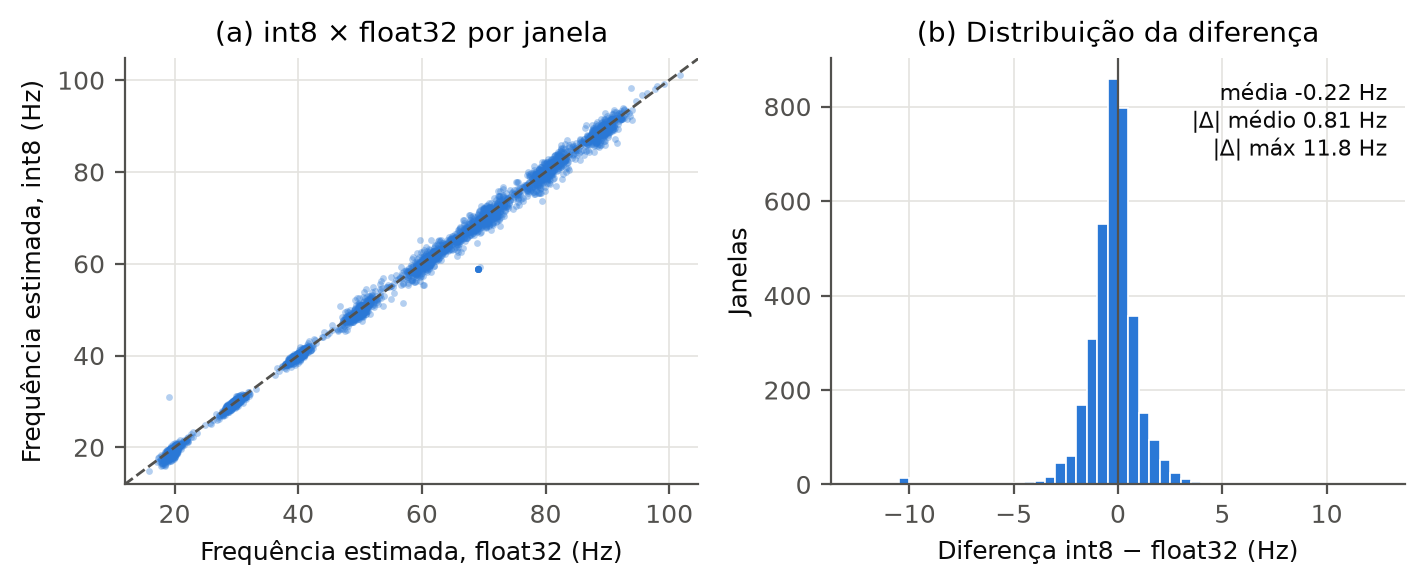
\includegraphics[width=\textwidth]{figs/embarcado/fig_quantizacao.png}
	\caption{Efeito da quantização int8 sobre a frequência estimada nas 3\,540 janelas: (a) estimativa int8 contra float32, com a reta identidade tracejada; (b) distribuição da diferença.}
	\label{sim:fig:quantizacao}
\end{figure}

\begin{table}[htbp]
	\centering
	\small
	\caption{Concordância entre implementações (3\,540 janelas). ``Nível'' é a frequência arredondada a 10\,Hz.}
	\label{sim:tab:fidelidade}
	\begin{tabular}{L{0.42\textwidth}ccc}
		\toprule
		\textbf{Comparação} & \textbf{Classe igual} & \textbf{Nível igual} & \textbf{\(|\Delta f|\) máx.} \\
		\midrule
		C float32 \(\times\) \texttt{scikit-learn} & 100\,\% & 100\,\% & \(2{,}5\times10^{-4}\)\,Hz \\
		C int8 \(\times\) emulação int8 (Python) & 100\,\% & 100\,\% & 0 (bit a bit) \\
		int8 \(\times\) float32 (efeito da quantização) & 98,2\,\% & 96,6\,\% & 11,8\,Hz \\
		Cadeia em C, percentis exatos \(\times\) Python int8 & 100\,\% & 100\,\% & 1,2\,Hz \\
		Cadeia em C, histograma \(\times\) Python int8 & 97,4\,\% & 96,2\,\% & 6,4\,Hz \\
		\bottomrule
	\end{tabular}
\end{table}

\subsubsection{Descritores e cadeia completa (V2)}

As fórmulas da Equação~\eqref{sim:eq:conversao}, aplicadas aos campos brutos, reproduziram as colunas físicas do \texttt{hits.csv} com erro relativo de no máximo \(10^{-5}\), compatível com o arredondamento do próprio arquivo. A Figura~\ref{sim:fig:descritores} mostra o erro normalizado máximo de cada descritor, nos dois canais, partindo do registro bruto. No modo exato, todos os erros ficaram abaixo de \(10^{-5}\), no nível da precisão simples; taxas e frações foram exatas, e os valores NaN coincidiram em todas as janelas. No modo histograma, os percentis ficaram acima da tolerância, como esperado de uma quantização em classes de largura fixa, com erros de até 0,2\,dB na amplitude, 0,04 nos logaritmos e 1,5\,kHz na frequência média.

\begin{figure}[htbp]
	\centering
	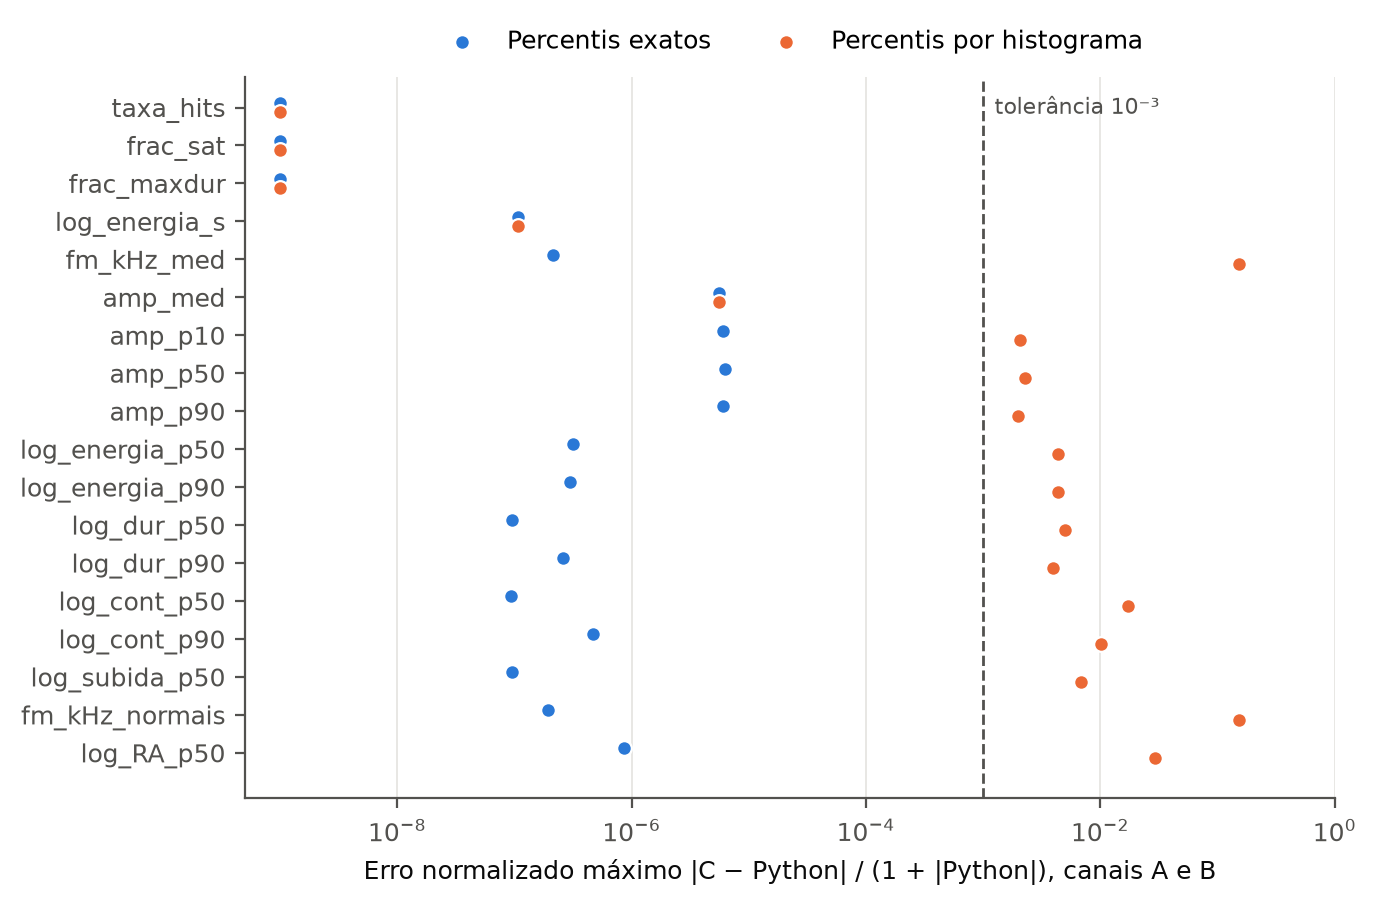
\includegraphics[width=0.92\textwidth]{figs/embarcado/fig_erro_descritores.png}
	\caption{Erro normalizado máximo, \(|x_{\mathrm{C}} - x_{\mathrm{Py}}|/(1+|x_{\mathrm{Py}}|)\), de cada descritor calculado em C a partir do registro bruto, nos dois modos de percentis, sobre as 3\,540 janelas e os dois canais. Erros nulos são desenhados em \(10^{-9}\). A linha tracejada é a tolerância de \(10^{-3}\).}
	\label{sim:fig:descritores}
\end{figure}

O que importa para a aplicação é a saída das redes. Com percentis exatos, a cadeia completa em C devolveu a mesma classe e o mesmo nível de frequência que o Python em 100\,\% das janelas; a maior diferença de frequência, 1,2\,Hz, vem do arredondamento da amplitude no \texttt{hits.csv}, que o C não usa ao partir do registro bruto. Com histogramas, a classe coincidiu em 97,4\,\% e o nível em 96,2\,\% (Tabela~\ref{sim:tab:fidelidade}), uma perda comparável à da própria quantização.

\subsubsection{Núcleo em lógica dedicada (V3 e V4)}

A simulação C e a cossimulação C/RTL do núcleo HLS, com 256 janelas, terminaram sem nenhuma divergência nos acumuladores ou na classe. A latência das duas redes foi de 11\,391 ciclos na síntese e de 11\,268 a 11\,393 ciclos na cossimulação, ou cerca de 114\,\(\mu\)s a 100\,MHz. Cada neurônio custa o número de entradas mais cerca de 12 ciclos de enchimento do \textit{pipeline}.

A Tabela~\ref{sim:tab:recursos} compara a estimativa da síntese HLS com o resultado após posicionamento e roteamento fora de contexto. A temporização foi atendida com folga: o caminho crítico tem 6,84\,ns, o que admitiria cerca de 146\,MHz. A implementação ocupou bem menos LUTs que a estimativa (656 contra 2\,421), porque a síntese lógica absorve parte da lógica de controle, e mais DSPs (14 contra 10), por causa da multiplicação de 64 bits da requantização. Os 3,5 blocos de BRAM guardam os 8\,960 pesos int8 das duas redes.

\begin{table}[htbp]
	\centering
	\small
	\caption{Recursos do IP HLS no XC7A35T (100\,MHz).}
	\label{sim:tab:recursos}
	\begin{tabular}{lrrrr}
		\toprule
		\textbf{Recurso} & \textbf{Estimativa HLS} & \textbf{Pós-roteamento} & \textbf{Disponível} & \textbf{Uso} \\
		\midrule
		LUT & 2\,421 & 656 & 20\,800 & 3,2\,\% \\
		\textit{Flip-flops} & 1\,648 & 682 & 41\,600 & 1,6\,\% \\
		DSP48E1 & 10 & 14 & 90 & 15,6\,\% \\
		BRAM (blocos de 36\,kb) & 3,5 & 3,5 & 50 & 7,0\,\% \\
		Período (ns) & 7,00 & 6,84 & 10,00 (alvo) & --- \\
		\bottomrule
	\end{tabular}
\end{table}

\subsubsection{Programa na MicroBlaze (V5)}

As seis simulações RTL (três programas \(\times\) duas configurações do processador) terminaram com a mesma sequência de valores de resultado da execução no computador: mesmas classes, mesmos acumuladores e, no modo exato, nenhum descritor fora da tolerância. Isso confirma, no nível do processador, que o binário embarcado reproduz o modelo. A Tabela~\ref{sim:tab:ciclos} resume os ciclos medidos.

\begin{table}[htbp]
	\centering
	\small
	\caption{Ciclos medidos na simulação RTL da MicroBlaze (100\,MHz, memória local, sem caches). Com FPU, médias sobre 2 vetores (MLP) e 2 janelas reais com 163 \textit{hits} (cadeia); sem FPU, 1 vetor e 1 janela com 81 \textit{hits}.}
	\label{sim:tab:ciclos}
	\begin{tabular}{lrr}
		\toprule
		\textbf{Etapa} & \textbf{Sem FPU} & \textbf{Com FPU} \\
		\midrule
		MLP float32, duas redes & \mbMlpFloatSoft & \mbMlpFloatFpu \\
		Quantização da entrada & \mbQuantSoft & \mbQuantFpu \\
		Núcleo int8, duas redes & \mbMlpIntSoft & \mbMlpIntFpu \\
		Inferência int8 completa (\(\mu\)s) & \mbMlpIntSoftUs & \mbMlpIntFpuUs \\
		\midrule
		Por \textit{hit}, modo exato & \mbHitSoft & \mbHitFpu \\
		Por \textit{hit}, modo histograma & \mbHitHistSoft & \mbHitHistFpu \\
		Fechar a janela, modo exato & \mbFecharSoft & \mbFecharFpu \\
		Fechar a janela, modo histograma & \mbFecharHistSoft & \mbFecharHistFpu \\
		\bottomrule
	\end{tabular}
\end{table}

\mbParagrafoMlp

A Figura~\ref{sim:fig:latencia} compara a latência da inferência nas plataformas. A Figura~\ref{sim:fig:ciclosjanela} decompõe o custo de uma janela típica dos dados (cerca de 80 \textit{hits}), e a Figura~\ref{sim:fig:carga} extrapola, a partir dos ciclos medidos, a ocupação da CPU em função da taxa de \textit{hits}.

\begin{figure}[htbp]
	\centering
	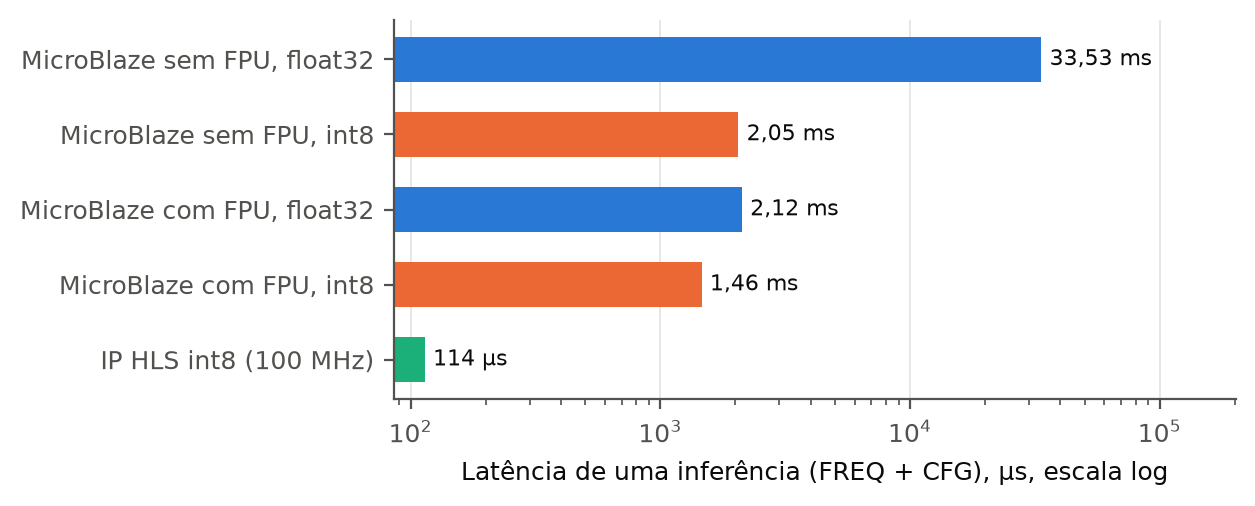
\includegraphics[width=0.85\textwidth]{figs/embarcado/fig_latencia_mlp.png}
	\caption{Latência de uma inferência (regressor e classificador) na MicroBlaze, medida em simulação RTL, e no IP HLS, medida na cossimulação. A MicroBlaze int8 inclui a quantização da entrada.}
	\label{sim:fig:latencia}
\end{figure}

\begin{figure}[htbp]
	\centering
	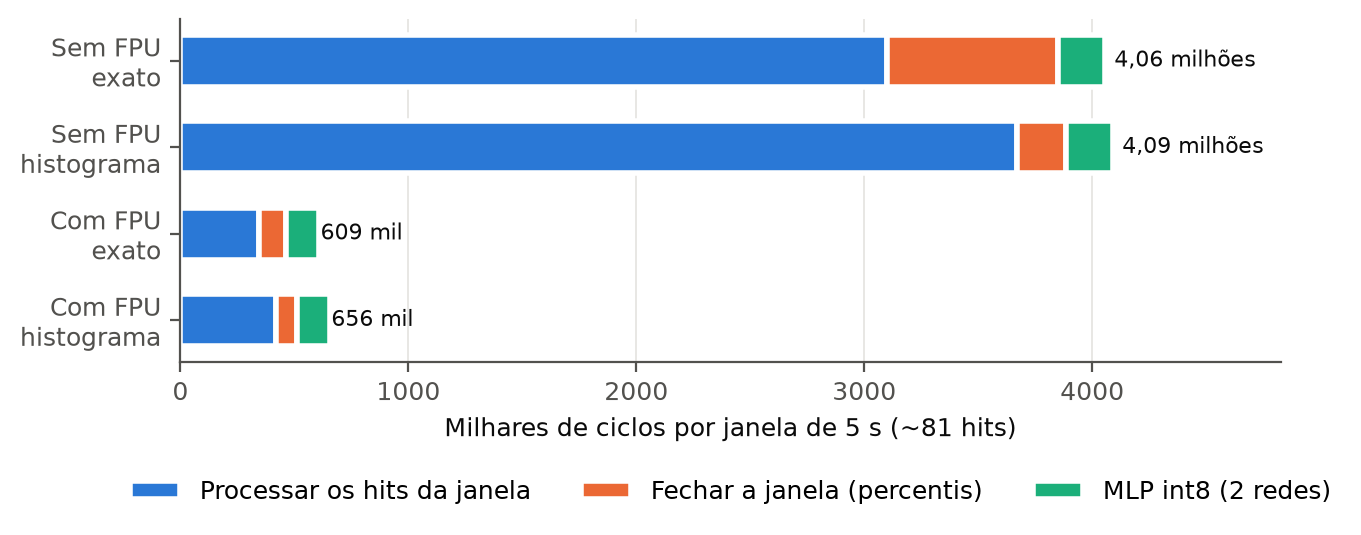
\includegraphics[width=0.92\textwidth]{figs/embarcado/fig_ciclos_janela.png}
	\caption{Composição dos ciclos de uma janela de 5\,s na MicroBlaze, para uma janela real de 81 \textit{hits} (custos por \textit{hit} medidos): processamento dos \textit{hits}, fechamento da janela (percentis) e MLP int8.}
	\label{sim:fig:ciclosjanela}
\end{figure}

\begin{figure}[htbp]
	\centering
	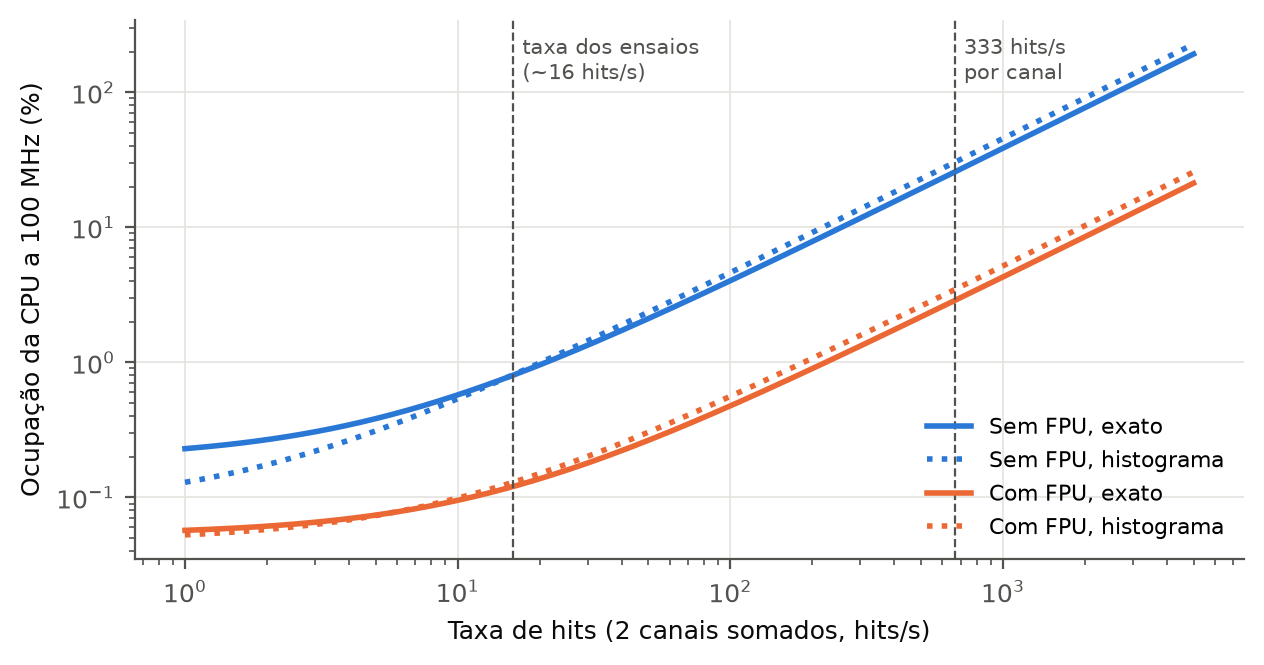
\includegraphics[width=0.85\textwidth]{figs/embarcado/fig_carga_cpu.png}
	\caption{Ocupação da CPU da MicroBlaze a 100\,MHz pela cadeia embarcada em função da taxa de \textit{hits}, extrapolada dos ciclos medidos por \textit{hit}, por fechamento de janela e pela MLP. As linhas verticais marcam a taxa dos ensaios da bomba e a maior taxa sustentada em ensaio elétrico. No modo exato, o fechamento da janela foi medido com cerca de 80 \textit{hits} e cresce como \(n \log n\); a extrapolação o subestima em taxas altas, e acima de 1\,024 \textit{hits} por canal por janela (cerca de 205 \textit{hits}/s por canal) o modo exato deixa de se aplicar.}
	\label{sim:fig:carga}
\end{figure}

\mbParagrafoCarga

A Tabela~\ref{sim:tab:memoria} resume a memória. O binário de teste da cadeia, com a MLP int8 e sem o caminho float32, ocupa de \mbTextoMin{} a \mbTextoMax\,kB de código e constantes, incluindo cerca de 10\,kB de \textit{hits} de teste que não existem no firmware real.

\begin{table}[htbp]
	\centering
	\small
	\caption{Memória da cadeia embarcada (ELF de teste, \texttt{mb-gcc} 2022.2, \texttt{-O2}).}
	\label{sim:tab:memoria}
	\begin{tabular}{lrr}
		\toprule
		\textbf{Item} & \textbf{Sem FPU} & \textbf{Com FPU} \\
		\midrule
		Código e constantes, modo exato (kB) & \mbTextoExatoSoft & \mbTextoExatoFpu \\
		Código e constantes, modo histograma (kB) & \mbTextoHistSoft & \mbTextoHistFpu \\
		Estado da janela, modo exato (kB) & 65,6 & 65,6 \\
		Estado da janela, modo histograma (kB) & 10,3 & 10,3 \\
		Pesos int8 e vieses das duas redes (kB) & \(\approx 9{,}8\) & \(\approx 9{,}8\) \\
		Pesos float32 das duas redes, se usados (kB) & \(\approx 37\) & \(\approx 37\) \\
		\bottomrule
	\end{tabular}
\end{table}

% =======================================================================================================
\subsection{Discussão}
\label{sim:sec:discussao}

\subsubsection{Qual rota usar}

A Tabela~\ref{sim:tab:rotas} reúne o custo em lógica de cada alternativa. Os números da MicroBlaze vêm da síntese do mesmo sistema usado na simulação e servem para dimensionar o acréscimo da FPU; o processador em si já existe no MOMEA e não é um custo da cadeia.

\begin{table}[htbp]
	\centering
	\small
	\caption{Recursos lógicos no XC7A35T: núcleo da MicroBlaze (síntese) e IP HLS (pós-roteamento).}
	\label{sim:tab:rotas}
	\begin{tabular}{lrrrr}
		\toprule
		\textbf{Bloco} & \textbf{LUT} & \textbf{FF} & \textbf{DSP} & \textbf{BRAM (36\,kb)} \\
		\midrule
		MicroBlaze sem FPU (núcleo) & 1\,361 & 857 & 4 & --- \\
		MicroBlaze com FPU estendida (núcleo) & 2\,322 & 1\,599 & 6 & --- \\
		Acréscimo da FPU & 961 & 742 & 2 & --- \\
		IP HLS int8 (duas redes) & 656 & 682 & 14 & 3,5 \\
		Memória local de 128\,kB (sistema simulado) & 17 & 16 & --- & 32 \\
		\bottomrule
	\end{tabular}
\end{table}

Para a aplicação atual, uma decisão a cada 5\,s, as duas rotas sobram. \mbParagrafoRota{} O IP HLS é \mbFatorHls{} vezes mais rápido que a MicroBlaze sem FPU e libera o processador, ao custo de 14 DSPs e 3,5 blocos de BRAM; ele se justificaria para classificar cada \textit{hit} em taxas altas, para modelos maiores ou se a MicroBlaze já estiver saturada pela pilha de rede. Em qualquer caso, a parte cara da cadeia não é a rede, mas o processamento por \textit{hit}, dominado pelos logaritmos; esse custo é o mesmo nas duas rotas, porque os descritores ficam no processador. Se a taxa de \textit{hits} crescer muito, o próximo passo natural é calcular na lógica as grandezas por \textit{hit} (incluindo os logaritmos, por tabela) e deixar à MicroBlaze apenas o fechamento da janela.

Entre os modos de percentis, o exato é preferível enquanto a janela couber na memória, porque preserva a decisão do modelo de referência em todas as janelas. O histograma troca cerca de 2,6\,\% de classes diferentes por memória constante e custo por \textit{hit} independente da taxa. Histogramas mais finos reduziriam essa diferença.

\subsubsection{O que a simulação garante}

A cadeia de verificação estabelece, com critérios explícitos, que: (i) a exportação do modelo e a implementação em C reproduzem o modelo de referência, bit a bit no caso int8; (ii) os descritores calculados em C a partir do registro bruto reproduzem os da Seção~\ref{sec:mm_bomba}; (iii) o RTL gerado pelo HLS é funcionalmente idêntico ao C e fecha a temporização na peça do MOMEA; e (iv) o binário compilado para a MicroBlaze produz os mesmos resultados em um processador simulado no nível RTL, com custo de tempo medido em ciclos.

A simulação não cobre, porém, o que depende da placa e do sistema completo:
\begin{itemize}
	\item a integração com o projeto atual do MOMEA, cuja ocupação de recursos não foi verificada; os recursos do IP foram obtidos fora de contexto, e o sistema MicroBlaze simulado não é o do MOMEA;
	\item o tempo de parede no firmware real, com caches ou memória externa, interrupções, recepção dos registros e pilha UDP concorrendo pelo processador;
	\item a base de tempo da janela: no treino, as janelas usaram a hora de chegada dos registros no computador; na placa, usarão o relógio local. Com o carimbo de tempo de \textit{hardware} ainda não implementado, pequenas diferenças na fronteira das janelas são esperadas;
	\item o comportamento elétrico do \textit{front-end} e do conversor, incluindo a saturação observada nos ensaios da bomba (Seção~\ref{sec:mm_bomba}).
\end{itemize}

\subsubsection{O modelo continua sendo o limite}

A implementação não muda a capacidade de generalização do modelo. Na Seção~\ref{sec:res_bomba}, a frequência generalizou para corridas não vistas (erro médio de 4 a 6\,Hz), mas a configuração das válvulas não (21 a 28\,\% de acurácia por corrida deixada de fora, para 14\,\% de acaso), e os dados têm limitações sérias: uma única corrida por condição, ordem fixa, limiar variável entre sessões e 70\,\% dos \textit{hits} saturados (Seção~\ref{sec:mm_bomba}). A contribuição deste trabalho é a infraestrutura: um fluxo que leva qualquer modelo do mesmo formato do Python ao FPGA, com verificação automática em cada nível. Retreinar com dados melhores exige apenas regenerar os cabeçalhos e repetir os testes; o código e o \textit{hardware} não mudam.

% =======================================================================================================


% -------------------------------------------------------------------------------------------------------
\section{Validação externa na base CWRU}
\label{sec:res_cwru}
% Gerado por ferramentas/importar_relatorios.py a partir de CWRU/RELATORIO_CWRU-10.11.2026/RELATORIO_CWRU.tex.
% Revisado à mão na dissertação: edite este arquivo, não a fonte.
\subsection{Resultados}
\label{cwru:sec:resultados}

\subsubsection{Os \textit{hits} capturam a física do defeito, mas só com limiar flutuante}

A Figura~\ref{cwru:fig:sinais} mostra trechos de 60\,ms das quatro condições, com os \textit{hits} detectados. Na pista externa, os impactos são nítidos e espaçados de cerca de 9\,ms, mas o anel de cada impacto permanece acima de 0,3\,\(g\) por vários milissegundos. Na pista interna, com RMS de 0,58\,\(g\), o sinal fica acima do limiar fixo quase o tempo todo. Com limiar fixo, os impactos se fundem: na gravação IR de 0,007~polegada com carga 0, 95\,\% dos \textit{hits} foram truncados pela duração máxima, e em três das quatro gravações IR de 0,021~polegada, cerca de 50\,\%. É o mesmo regime de emissão contínua observado nos ensaios da bomba. Com o limiar flutuante, a fração truncada caiu para no máximo 1\,\% em todas as gravações.

\begin{figure}[htbp]
	\centering
	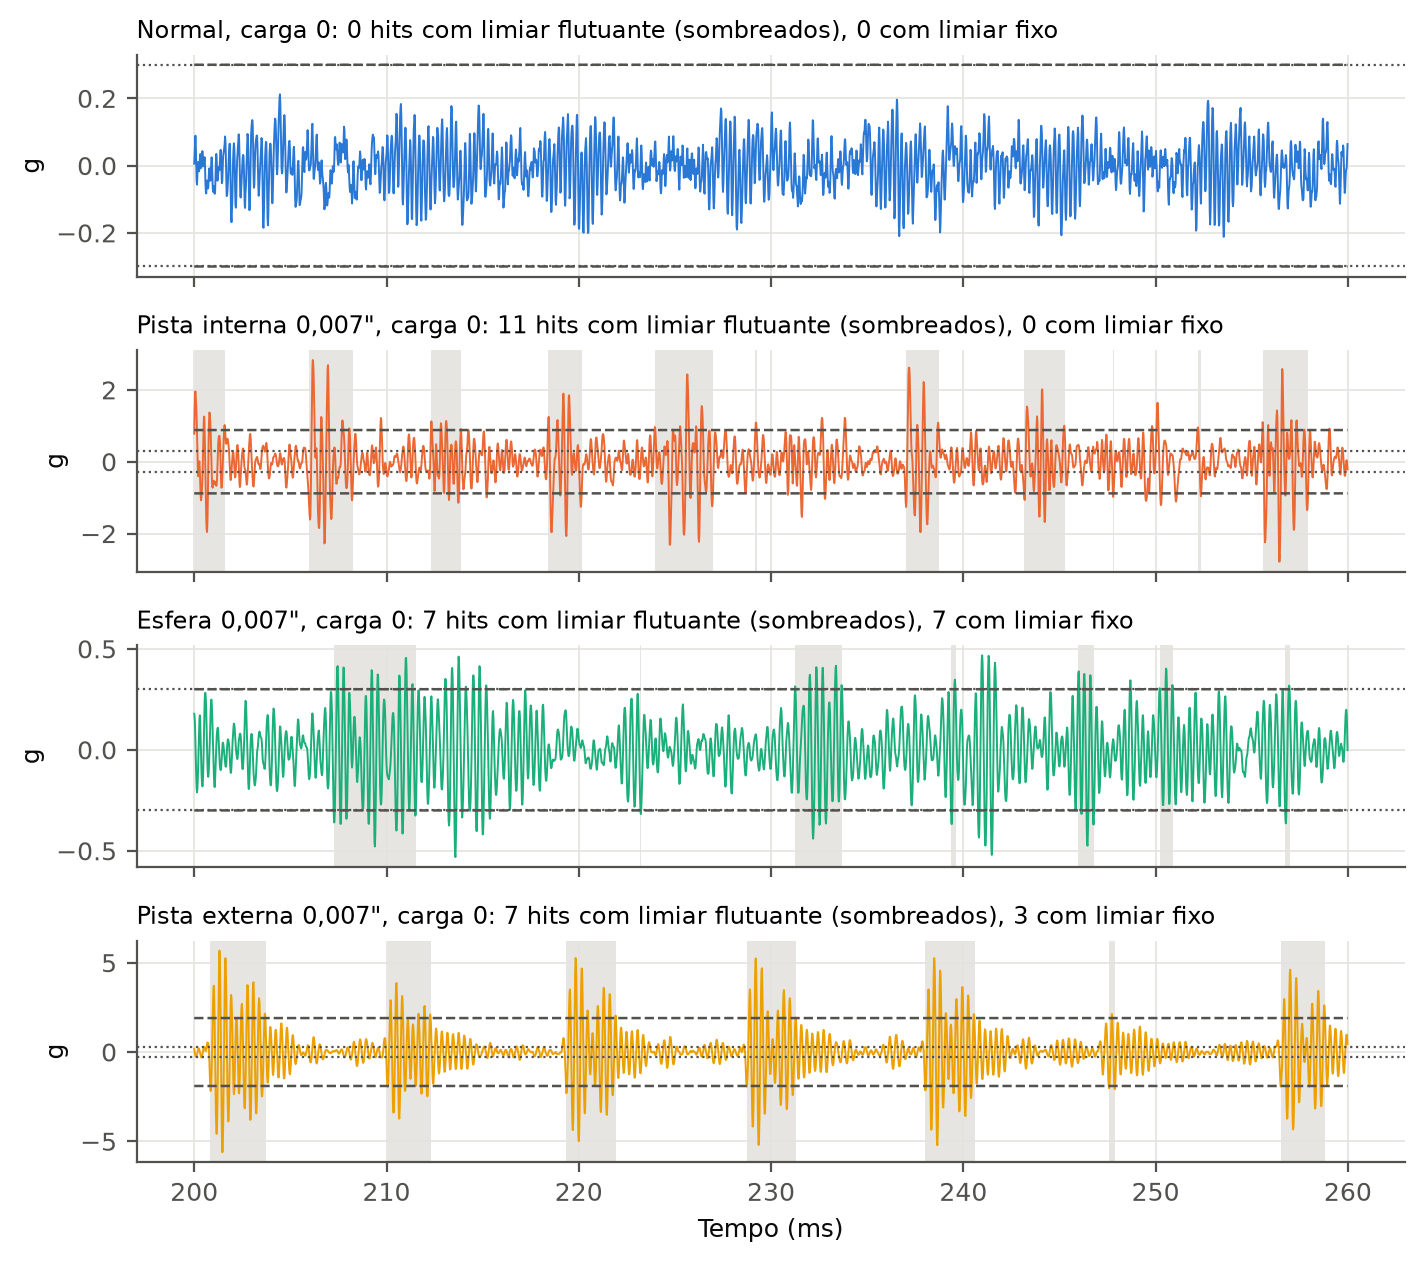
\includegraphics[width=\textwidth]{figs/cwru/fig_sinais_hits.png}
	\caption{Trechos de 60\,ms das quatro condições (carga 0, diâmetro de 0,007~polegada). Linhas pontilhadas: limiar fixo de 0,3\,\(g\); tracejadas: limiar flutuante. Áreas sombreadas: \textit{hits} detectados com o limiar flutuante.}
	\label{cwru:fig:sinais}
\end{figure}

A Figura~\ref{cwru:fig:ordem} mostra a ordem do intervalo entre \textit{hits}. Com limiar fixo, as distribuições são largas e têm picos espúrios perto de 1 e 2, que vêm de \textit{hits} fundidos e truncados. Com limiar flutuante, a pista externa concentra-se em 3,60 (BPFO = 3,58) e a pista interna em 5,27 (BPFI = 5,42); o pequeno desvio da pista interna é compatível com impactos perdidos quando o defeito sai da zona de carga. A esfera fica dispersa em torno de 5,5, longe de 2\(\times\)BSF = 4,71, o que concorda com a dificuldade conhecida de diagnosticar os defeitos de esfera dessa base \cite{smith2015}. Esse descritor é obtido sem FFT, apenas com os instantes dos \textit{hits}, o que reforça a importância do carimbo de tempo de \textit{hardware} ainda pendente no MOMEA.

\begin{figure}[htbp]
	\centering
	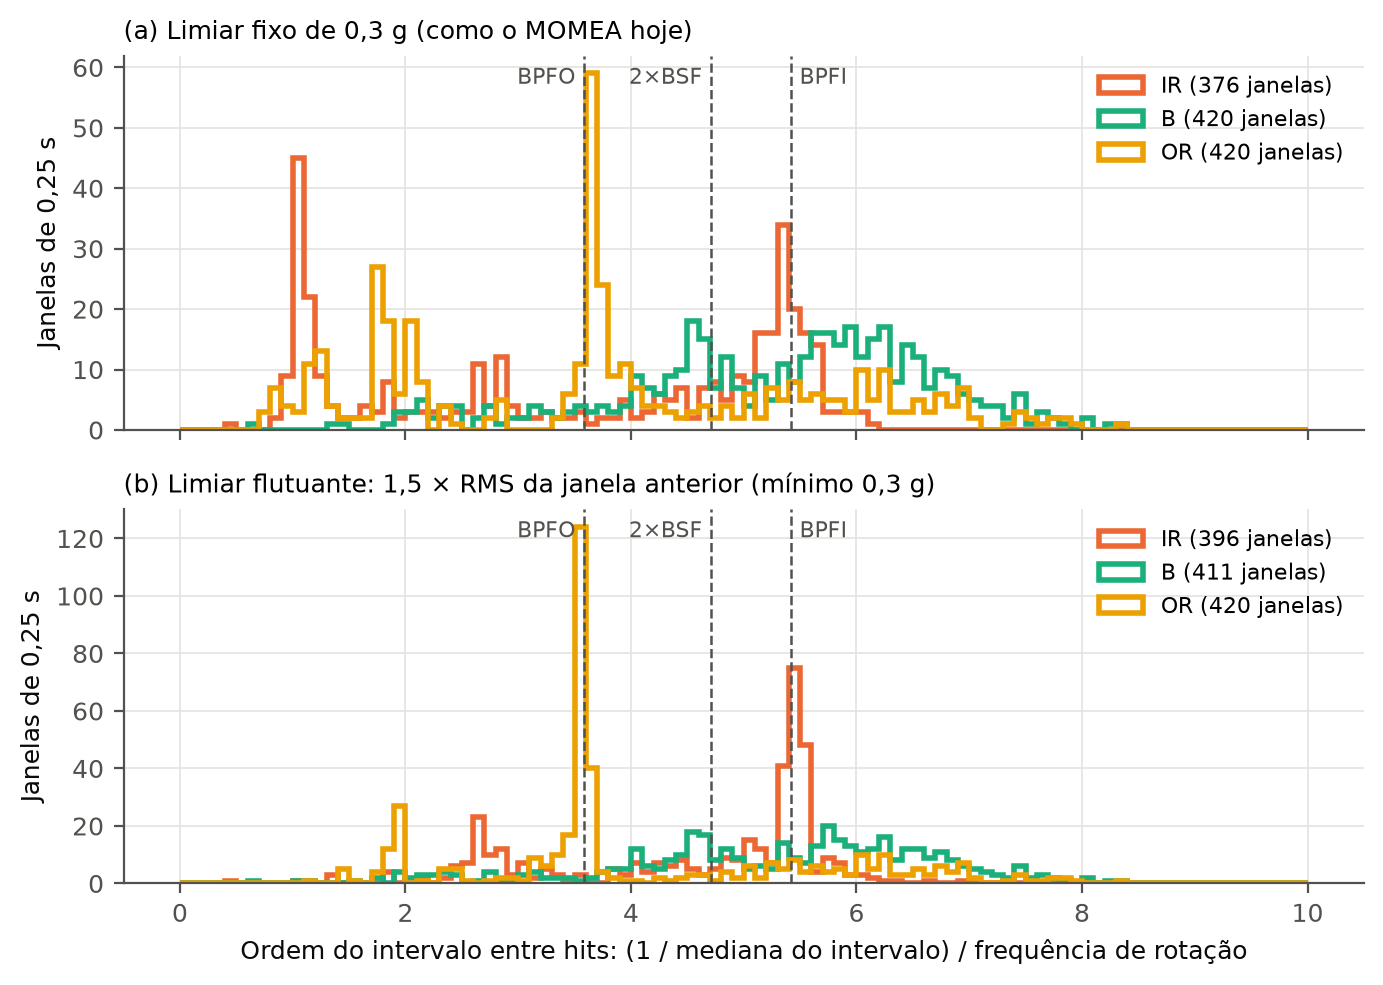
\includegraphics[width=\textwidth]{figs/cwru/fig_ordem_ihi.png}
	\caption{Ordem do intervalo entre \textit{hits} por janela, (a) com limiar fixo e (b) com limiar flutuante. Linhas tracejadas: frequências de defeito teóricas em múltiplos da rotação.}
	\label{cwru:fig:ordem}
\end{figure}

\subsubsection{A acurácia depende da validação}

A Figura~\ref{cwru:fig:acuracia} e a Tabela~\ref{cwru:tab:acuracia} resumem a classificação em quatro classes. Com janelas sorteadas, todos os grupos chegaram a 87--92\,\%, e as diferenças entre eles são pequenas. Deixar uma carga de fora quase não mudou o quadro (82--90\,\%), o que, à primeira vista, sugeriria boa generalização. Não é o caso: o teste ainda contém os mesmos rolamentos físicos, gravados em outra carga.

Quando o diâmetro inteiro sai do treino, a acurácia cai para perto do acaso nos descritores de amplitude: 21\,\% para os clássicos e 25\,\% para os \textit{hits} com limiar fixo, com a MLP. Os \textit{hits} com limiar flutuante sustentaram 46\,\% (53\,\% com RF), e o envelope, que mede diretamente as frequências de defeito, 63\,\%. Juntar todos os descritores não ajudou a MLP (41\,\%): os descritores de amplitude dominam o ajuste e não se transferem entre rolamentos, porque a severidade não é monotônica. Por exemplo, o defeito de 0,014~polegada na pista externa tem RMS de 4 a 8 vezes menor que os de 0,007 e 0,021. Na tarefa de dez classes, a queda das janelas sorteadas para a carga de fora foi um pouco maior (por exemplo, de 91 para 87\,\% com todos os descritores).

\begin{figure}[htbp]
	\centering
	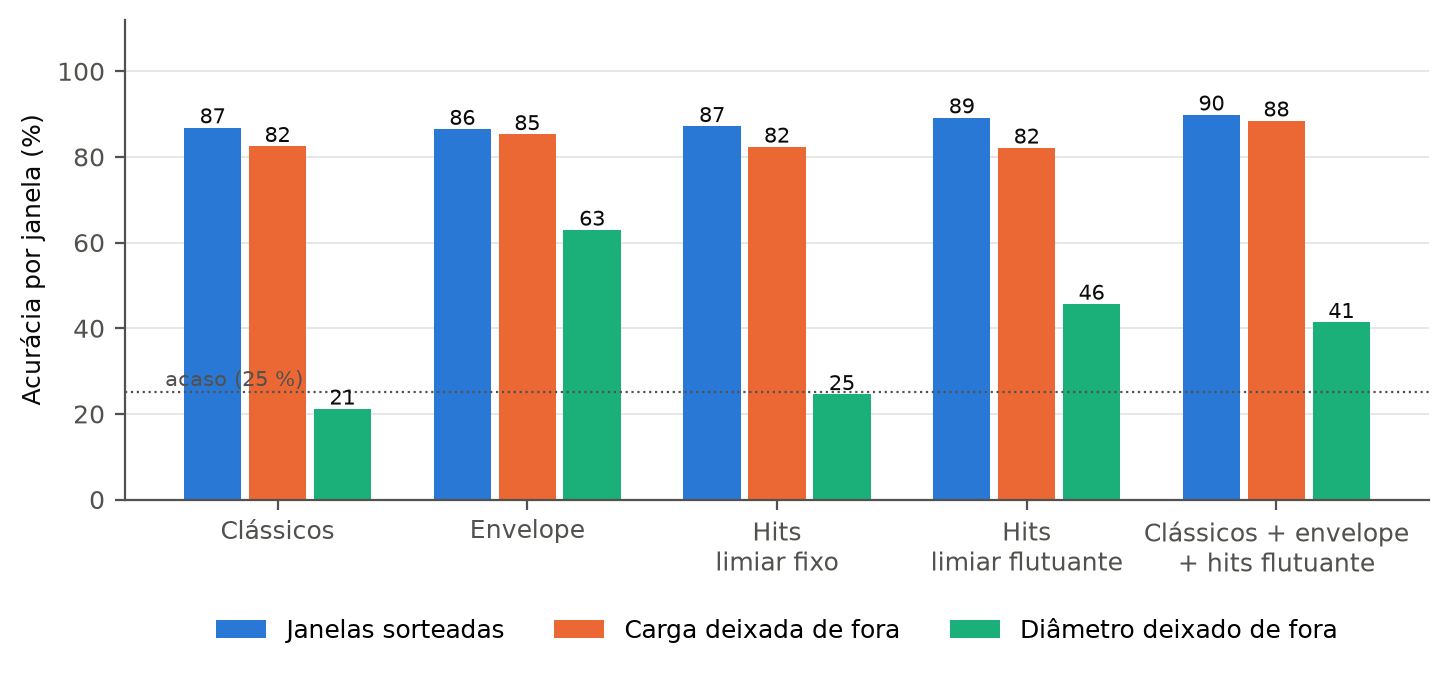
\includegraphics[width=\textwidth]{figs/cwru/fig_acuracia_validacoes.png}
	\caption{Acurácia por janela da MLP em quatro classes, por grupo de descritores e validação. A linha pontilhada marca o acaso (25\,\%).}
	\label{cwru:fig:acuracia}
\end{figure}

\begin{table}[htbp]
	\centering
	\small
	\caption{Acurácia por janela em quatro classes (entre parênteses, por gravação, com voto majoritário).}
	\label{cwru:tab:acuracia}
	\begin{tabular}{llccc}
		\toprule
		\textbf{Descritores} & \textbf{Modelo} & \textbf{Sorteada} & \textbf{Carga de fora} & \textbf{Diâmetro de fora} \\
		\midrule
		Clássicos & MLP & 86,8 (87,5) & 82,5 (82,5) & 21,2 (25,6) \\
		 & RF & 89,5 (92,5) & 86,4 (87,5) & 28,4 (28,2) \\
		Envelope & MLP & 86,5 (90,0) & 85,2 (90,0) & \textbf{62,9} (66,7) \\
		 & RF & 87,4 (90,0) & 85,8 (90,0) & 58,0 (59,0) \\
		\textit{Hits}, limiar fixo & MLP & 87,1 (90,0) & 82,3 (85,0) & 24,6 (20,5) \\
		 & RF & 88,7 (95,0) & 84,4 (80,0) & 35,3 (38,5) \\
		\textit{Hits}, limiar flutuante & MLP & 89,2 (92,5) & 82,1 (82,5) & 45,7 (43,6) \\
		 & RF & 90,5 (92,5) & 87,9 (90,0) & 53,3 (51,3) \\
		Todos (flutuante) & MLP & 89,8 (90,0) & 88,4 (87,5) & 41,4 (38,5) \\
		 & RF & 91,9 (90,0) & 89,6 (87,5) & 54,3 (51,3) \\
		\bottomrule
	\end{tabular}
\end{table}

A Figura~\ref{cwru:fig:confusao} mostra onde os erros se concentram, para os \textit{hits} com limiar flutuante. A máquina sã é sempre reconhecida, porque não gera \textit{hits}; o problema está em distinguir os defeitos entre si. Com o diâmetro de fora, a pista externa é confundida principalmente com a interna, e a esfera se divide entre as três classes de defeito.

\begin{figure}[htbp]
	\centering
	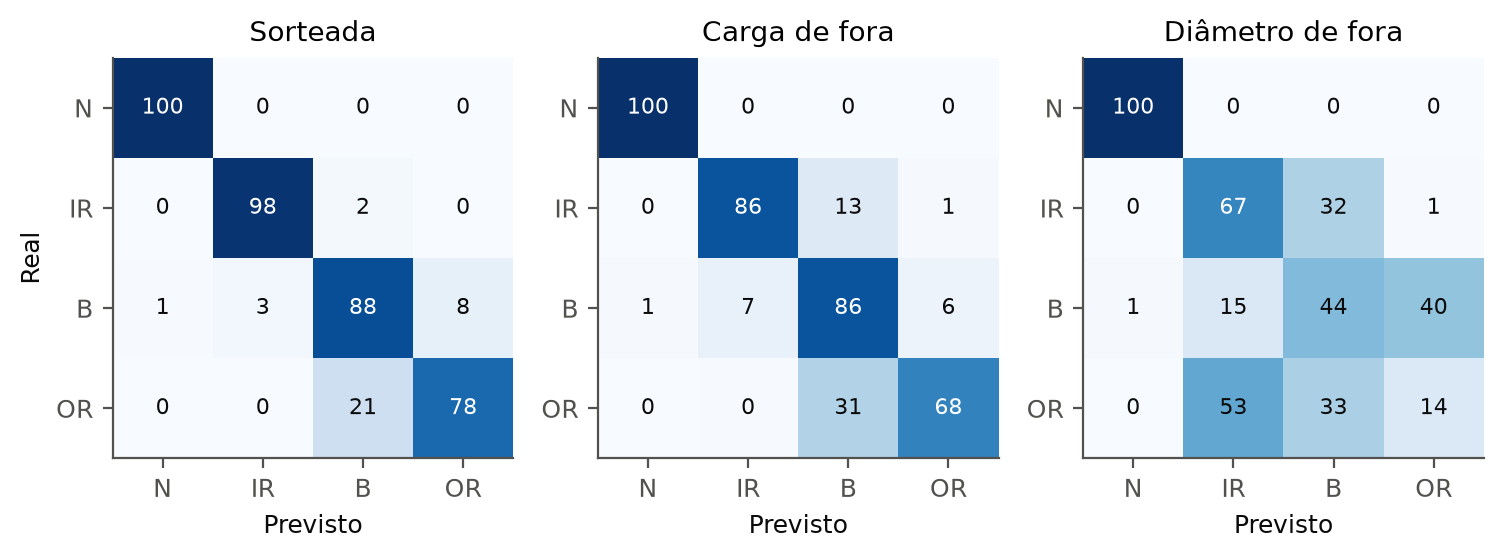
\includegraphics[width=\textwidth]{figs/cwru/fig_confusao_hits.png}
	\caption{Matrizes de confusão (\% por linha) da MLP com descritores de \textit{hits} e limiar flutuante, nas três validações.}
	\label{cwru:fig:confusao}
\end{figure}

\subsubsection{MLP int8}

Em cada parte da validação por carga, a MLP treinada foi quantizada para int8 com a mesma aritmética da implementação embarcada (Seção~\ref{sec:mm_embarcado}): escala de entrada fixa, pesos simétricos por camada e requantização inteira, com escalas calibradas apenas no treino da parte. A Tabela~\ref{cwru:tab:int8} mostra que a decisão int8 coincidiu com a de ponto flutuante em 98,4 a 100\,\% das janelas, e que a acurácia mudou no máximo 0,5 ponto percentual.

\begin{table}[htbp]
	\centering
	\small
	\caption{MLP em ponto flutuante e em int8 na validação por carga (quatro classes; faixas sobre as quatro partes).}
	\label{cwru:tab:int8}
	\setlength{\tabcolsep}{4pt}
	\begin{tabular}{lccccc}
		\toprule
		\textbf{Descritores} & \textbf{Entradas} & \textbf{MACs} & \textbf{Acc. float} & \textbf{Acc. int8} & \textbf{Concordância} \\
		\midrule
		\textit{Hits}, limiar flutuante & 14 & 3\,072 & 74,3--88,5\,\% & 73,8--88,2\,\% & 99,5--99,7\,\% \\
		Todos & 29 & 4\,032 & 86,5--90,5\,\% & 86,0--90,5\,\% & 98,4--100\,\% \\
		\bottomrule
	\end{tabular}
\end{table}

\subsubsection{Custo embarcado}

Os custos a seguir são estimativas derivadas dos ciclos medidos na simulação RTL da MicroBlaze a 100\,MHz (Seção~\ref{sec:mm_embarcado}), e não medições específicas para esta base:
\begin{itemize}
	\item \textbf{detecção dos \textit{hits}}: na lógica, como no MOMEA. A 48\,kHz, o detector é trivial para o FPGA;
	\item \textbf{descritores de \textit{hits}}: o custo medido foi de 4\,232 ciclos por \textit{hit} com FPU e 38\,287 sem. Na maior taxa observada (178 \textit{hits}/s), isso dá cerca de 0,8\,\% e 6,8\,\% da CPU, respectivamente;
	\item \textbf{MLP int8 com 14 entradas}: 3\,072 multiplicações-acumulações, ou cerca de 48 mil ciclos por janela (15,5 ciclos por operação, medidos), isto é, 0,5\,ms a cada 0,25\,s, ou 0,2\,\% da CPU;
	\item \textbf{envelope}: exige filtragem, transformada de Hilbert e FFT por janela. Com \(N = 16\,384\) pontos, cada FFT complexa custa cerca de \(5N\log_2 N \approx 1{,}1\) milhão de operações de ponto flutuante, e são necessárias pelo menos três. Isso dá da ordem de 3 a 4 milhões de operações por janela, ou 12 a 16 milhões por segundo. É inviável na MicroBlaze sem FPU e exigiria um núcleo de FFT na lógica.
\end{itemize}
Há, portanto, um compromisso claro: o envelope generaliza melhor entre rolamentos, mas custa uma FFT por janela; os \textit{hits} com limiar flutuante ficam a meio caminho, por uma fração do custo, e cabem na arquitetura atual do MOMEA.

% =======================================================================================================
\subsection{Discussão}
\label{cwru:sec:discussao}

\subsubsection{O que este estudo acrescenta à dissertação}

Os resultados reproduzem, numa base pública, as duas lições do estudo da bomba.
\begin{itemize}
	\item \textbf{A validação precisa separar as unidades físicas.} Janelas sorteadas e até cargas deixadas de fora deram 82--92\,\% com qualquer grupo de descritores, porque o modelo reconhece o rolamento, e não o tipo de defeito. Só separando os rolamentos a diferença entre os descritores aparece. É o mesmo padrão do LORO na bomba, em que a configuração das válvulas caiu de 89--95\,\% para 21--28\,\%. Na CWRU, porém, sabe-se que os defeitos são reais e localizados, de modo que a queda não pode ser atribuída à falta de efeito físico; ela vem da pouca diversidade de unidades (nove rolamentos com defeito e um são).
	\item \textbf{O limiar fixo do extrator falha diante de emissão contínua.} Com limiar fixo, os impactos se fundiram e foram truncados pela duração máxima, e os descritores de \textit{hits} ficaram no acaso fora da amostra. Com um limiar flutuante, os \textit{hits} recuperaram a periodicidade do defeito e a acurácia quase dobrou. Isso dá uma recomendação concreta para o MOMEA: oferecer um limiar flutuante na lógica, junto com a revisão do ganho já indicada pelos ensaios da bomba.
\end{itemize}

\subsubsection{Limitações}

\begin{itemize}
	\item Os sinais são de vibração, a 48\,kHz; nem os descritores nem as conclusões se transferem diretamente para EA de alta frequência ou para cavitação.
	\item O fator do limiar flutuante e o DDT foram escolhidos com base na concordância com as frequências de defeito, o que usa os rótulos; o ganho na validação por diâmetro pode estar ligeiramente otimista.
	\item Há apenas três partes na validação por diâmetro e nove rolamentos com defeito, de modo que as acurácias fora da amostra têm grande incerteza.
	\item Os defeitos são artificiais (eletroerosão) e únicos por condição; algumas gravações são atípicas, e os defeitos de esfera dessa base são sabidamente difíceis \cite{smith2015}.
	\item Os custos embarcados são estimativas a partir de medições em outra cadeia; o caminho completo para esta base não foi simulado em RTL.
\end{itemize}

% =======================================================================================================


% -------------------------------------------------------------------------------------------------------
\section{Discussão integrada}
\label{sec:discussao_integrada}

As seções anteriores avaliaram, separadamente, cada parte da cadeia. Esta seção as reúne em torno das perguntas que orientaram o trabalho, várias delas levantadas na qualificação.

\subsection{O que se ganha com a extração de \textit{hits} seguida de uma MLP?}

A extração de \textit{hits} resolve o problema de volume. Com registros de 32 bytes, o fluxo de um canal cai de 20\,MB/s para cerca de 26\,kB/s, incluindo os cabeçalhos de rede, na maior taxa ensaiada (redução global de cerca de 770 vezes; Seção~\ref{sec:res_extrator}). Isso dispensa a compactação contínua e a escrita de alta vazão que a plataforma USB exigia (Seção~\ref{sec:mm_antecedentes}) e permite transmitir por Ethernet a 100\,Mb/s. O extrator reproduziu as convenções temporais do sistema comercial e registrou de 99,94 a 99,96\,\% dos estímulos, sem perda na comunicação.

A extração, porém, não diz em que condição a máquina está. Um \textit{hit} é um evento; a condição aparece na estatística dos eventos ao longo do tempo. Por isso a classificação usa descritores por janela (taxa, percentis de amplitude, energia, duração, contagens e periodicidade), e não um limiar fixo sobre um único \textit{hit}. Nos ensaios da bomba, esses descritores permitiram estimar a frequência de rotação com erro médio de 4 a 6\,Hz em corridas não vistas (Seção~\ref{sec:res_bomba}). Na base CWRU, a ordem do intervalo entre \textit{hits} reproduziu as frequências teóricas de defeito dos rolamentos (Seção~\ref{sec:res_cwru}). Nenhum desses resultados seria obtido comparando cada \textit{hit} com um limiar.

\subsection{O sistema opera em tempo real?}

Depende da etapa. O extrator opera em tempo real: cada \textit{hit} é detectado e parametrizado na lógica, e o registro é emitido \(T_{\mathrm{DDT}} + T_{\mathrm{HLT}} = 2{,}25\,\mathrm{ms}\) após o último cruzamento, mais o serviço do DMA, do \textit{firmware} e da rede. Na plataforma USB, os dados passavam por um banco intermediário e eram analisados depois; com o extrator, os registros chegam à aplicação à medida que os eventos ocorrem.

A classificação, por construção, decide uma vez por janela. Com janelas de 5\,s, o atraso de decisão é de até 5\,s, mais o tempo de inferência, que é desprezível: de 1,5 a 2,1\,ms na MicroBlaze e 114\,\(\mu\)s no IP HLS (Seção~\ref{sec:res_embarcado}). Para o monitoramento de cavitação e de desgaste, cuja evolução ocorre em minutos ou horas, esse atraso é adequado. A janela é um compromisso entre estabilidade e rapidez: no estudo da bomba, janelas de 2\,s melhoraram ligeiramente o reconhecimento da frequência, mas aumentam a variância dos descritores quando a taxa de \textit{hits} é baixa.

\subsection{Quanto tempo de coleta é necessário para identificar uma condição?}

A resposta depende da taxa de \textit{hits}, porque os descritores são estatísticas da população de eventos. Nos ensaios da bomba, havia cerca de 30 a 50 \textit{hits} por canal em cada janela de 5\,s. Na base CWRU, com 60 a 180 impactos por segundo, janelas de 0,25\,s bastaram para estimar a periodicidade do defeito. Como regra prática, a janela precisa conter algumas dezenas de \textit{hits} e vários períodos do fenômeno de interesse. Em termos de coleta para \emph{treinar} o modelo, o fator limitante não foi a duração das gravações, mas o número de corridas independentes: com uma única corrida por condição, o modelo aprende a assinatura da corrida, e não a condição (Seções~\ref{sec:res_bomba} e~\ref{sec:res_cwru}).

\subsection{O FPGA tem capacidade para a cadeia completa?}

Para o fluxo de dados, sim: o detector processa as amostras a 10\,MSa/s na lógica, e a carga restante é proporcional à taxa de \textit{hits}, não à taxa de amostragem. Na MicroBlaze, a cadeia de descritores e a MLP ocupam menos de 1\,\% da CPU na taxa dos ensaios e cerca de 26\,\% sem FPU a 333 \textit{hits}/s por canal (Seção~\ref{sec:res_embarcado}).

Em recursos lógicos, a margem é pequena. Após a migração da FIFO para BRAM, o extrator de dois canais ocupa cerca de 92\,\% das LUTs do XC7A35T (Seção~\ref{sec:mm_implementacao}). O IP HLS da MLP acrescentaria 656 LUTs (3,2\,\%) e 14 DSPs, e a FPU da MicroBlaze, 961 LUTs (4,6\,\%). Ambas as opções caberiam, mas no limite, com risco para o fechamento temporal. A rota recomendada para o hardware atual é, portanto, a inferência int8 em software, na MicroBlaze já existente e sem FPU: ela não consome lógica adicional e cabe com folga no tempo disponível. O IP HLS e a FPU tornam-se justificáveis em um FPGA maior ou se a taxa de \textit{hits} crescer muito.

\subsection{Por que uma MLP, e não uma rede convolucional?}

Porque a entrada do classificador é um vetor de descritores, e não uma série temporal. A arquitetura proposta não transmite as amostras: o FPGA entrega registros de \textit{hits}, dos quais se calculam 36 descritores por janela. Uma rede convolucional unidimensional (CNN-1D) ou temporal exigiria a forma de onda, isto é, justamente o fluxo que se quer evitar. As redes convolucionais bidimensionais sobre espectrogramas, estudadas anteriormente no projeto, são compatíveis com a aquisição contínua, mas não com o processamento na borda proposto. A MLP é o modelo natural para um vetor curto de atributos, tem custo previsível (cerca de 4,6 mil multiplicações-acumulações por rede) e é simples de quantizar e de mapear em \textit{hardware}. Uma extensão possível é capturar seletivamente a forma de onda de alguns \textit{hits} e combiná-la com os descritores, o que é discutido como trabalho futuro.

\subsection{Como a MLP foi implementada no FPGA?}

Em vez de \textit{frameworks} como FINN ou hls4ml \cite{Umuroglu2017FINN,duarte2018}, que partem de modelos treinados em \textit{frameworks} de aprendizado profundo e visam redes maiores, optou-se por um núcleo próprio em C. O modelo do \texttt{scikit-learn} é exportado como tabelas de pesos int8, e um único código-fonte compila para a MicroBlaze e para o Vitis HLS. Isso manteve a aritmética sob controle a ponto de exigir igualdade bit a bit entre o Python, o C e o RTL gerado, o que um fluxo automatizado não garantiria com a mesma transparência.

\subsection{O que foi comparado e o que não foi}

A qualificação previa comparar a solução em FPGA com CPU e GPU quanto a eficiência, tempo de resposta e consumo. A comparação realizada foi entre as rotas viáveis no próprio FPGA (MicroBlaze sem e com FPU e acelerador HLS), com o computador como referência de exatidão. Comparar com uma GPU não faz sentido para duas redes de cerca de 4,6 mil operações cada, executadas uma vez a cada 5\,s: o custo é dominado pela transferência e pela inicialização, e não pelo cálculo. O consumo de energia não foi medido, porque exige a placa; as estimativas de potência das ferramentas de síntese não foram usadas como substitutas.

\subsection{Limites do que foi demonstrado}

Os resultados demonstram que o extrator é equivalente ao sistema comercial na faixa ensaiada, que os descritores de \textit{hits} contêm informação sobre a condição de operação e que a classificação pode ser executada no FPGA com fidelidade ao modelo de referência. Eles não demonstram que o sistema detecta cavitação em uma turbina. Os ensaios do extrator são elétricos, sem sensor nem propagação estrutural; o estudo da bomba tem uma única corrida por condição, saturação de 70\,\% dos \textit{hits} e limiar variável entre sessões; e a base CWRU é de vibração, com defeitos artificiais. Esses limites orientam os trabalhos futuros do Capítulo~\ref{chap:conclusoes}.


\chapter{Conclusões}
\label{chap:conclusoes}
% =======================================================================================================
% Capítulo 5 - Conclusões e trabalhos futuros
% =======================================================================================================

Esta dissertação propôs e avaliou uma arquitetura de processamento em FPGA para o monitoramento de falhas em motobombas por EA, na qual o sinal é reduzido a registros de \textit{hits} na própria lógica programável e a condição de operação é inferida por uma rede MLP a partir desses registros. O trabalho partiu de uma limitação concreta da plataforma de aquisição contínua do Projeto MOMEA, o volume de dezenas de gigabytes por hora, e chegou a uma cadeia que transmite poucos quilobytes por segundo e pode decidir na borda.

\section{Síntese das contribuições}

As contribuições podem ser resumidas em quatro resultados:

\begin{enumerate}[label=\textbf{\arabic*.}]
	\item \textbf{Extrator de \textit{hits} em FPGA equivalente a um sistema comercial.} O extrator, implementado no Artix-7 XC7A35T com as mesmas convenções temporais do Vallen AMSY-6, registrou de 99,94 a 99,96\,\% de 48\,303 estímulos em ensaio simultâneo com o instrumento comercial (que registrou de 96,8 a 97,6\,\%), sem perda na comunicação (0 em 48\,280 registros) e com amplitudes 0,47 a 0,76\,dB acima das do AMSY-6, diferença compatível com a tolerância de ganho dos pré-amplificadores. A redução do volume de dados foi de cerca de 770 vezes na maior taxa ensaiada.
	\item \textbf{Classificação a partir dos registros, com validação honesta.} Descritores de \textit{hits} agregados em janelas de 5\,s permitiram estimar a frequência de rotação da bomba com erro médio de 4 a 6\,Hz em corridas e séries não vistas. A configuração das válvulas, reconhecida com 89 a 95\,\% de acurácia quando a corrida aparecia no treino, caiu para 21 a 28\,\% quando a corrida inteira foi deixada de fora. O trabalho mostrou que essa diferença decorre do delineamento dos dados, e não do método, e propôs um novo delineamento.
	\item \textbf{Inferência embarcada verificada por simulação.} O cálculo dos descritores e duas MLPs quantizadas em int8 foram implementados com um único código-fonte para a MicroBlaze e para o Vitis HLS. A implementação reproduziu o modelo de referência bit a bit e, com percentis exatos, a mesma decisão em 100\,\% das 3\,540 janelas. Na simulação RTL do processador, a inferência levou cerca de 2\,ms sem FPU; o IP HLS, 114\,\(\mu\)s, com 656 LUTs após o roteamento. Para o FPGA atual, já com cerca de 92\,\% das LUTs ocupadas pelo extrator, a rota recomendada é a inferência em software na MicroBlaze existente.
	\item \textbf{Validação externa em base pública.} Na base de rolamentos CWRU, os \textit{hits} detectados com limiar flutuante recuperaram as frequências teóricas de defeito, e a validação que separa rolamentos físicos reduziu a acurácia de 87--92\,\% para 21--63\,\%, reproduzindo, em dados de referência, a lição de validação do estudo da bomba.
\end{enumerate}

Duas lições atravessam os resultados. A primeira é que a acurácia de um diagnóstico só tem significado quando a validação separa as unidades físicas independentes: corridas, sessões ou rolamentos. A segunda é que o limiar fixo do extrator falha diante de emissão contínua: na bomba, com 70\,\% dos \textit{hits} saturados e muitos truncados pela duração máxima, e na CWRU, em que até 95\,\% dos \textit{hits} de uma gravação foram truncados com limiar fixo e nenhum com limiar flutuante.

\section{Limitações}

\begin{itemize}
	\item Os ensaios do extrator são elétricos e posteriores ao ponto de injeção; não incluem sensor, acoplamento, propagação estrutural nem cavitação. A referência elétrica medida, as repetições independentes e a varredura de amplitude e de ruído ainda não foram feitas.
	\item O carimbo de tempo de \textit{hardware} não está implementado, o que limitou a associação entre estímulos e registros ao nível de bloco e impede, por ora, o uso dos instantes dos \textit{hits} medidos no próprio FPGA.
	\item Os dados da bomba têm uma corrida por condição, ordem fixa, limiar variável entre sessões e saturação do conversor; com o ganho de 34\,dB, o limite do conversor corresponde a cerca de 102 a 103\,dB\(_{\mathrm{AE}}\).
	\item A inferência embarcada não foi executada na placa; o tempo de parede com a pilha de rede ativa, o consumo de energia e a integração com o \textit{firmware} real dependem do ensaio em \textit{hardware}.
	\item A base CWRU é de vibração, com defeitos artificiais e poucas unidades físicas; o fator do limiar flutuante foi ajustado com o auxílio dos rótulos.
\end{itemize}

\section{Trabalhos futuros}

Em ordem de dependência, os próximos passos são:
\begin{enumerate}[label=\textbf{\arabic*.}]
	\item implementar o carimbo de tempo de \textit{hardware} e um limiar flutuante no extrator, ambos de baixo custo em lógica;
	\item completar a caracterização metrológica do extrator (referência elétrica, divisor, pré-amplificador, repetições independentes e ensaios próximos ao limiar e à saturação);
	\item revisar o ganho do \textit{front-end}, ou adotar ganho ajustável, e estudar filtros passa-banda que separem o ruído da bomba das componentes associadas a vórtices e à cavitação;
	\item repetir o ensaio da bomba com várias corridas por condição, ordem aleatória, limiar fixo e uma medida independente do estado de cavitação;
	\item integrar a inferência ao \textit{firmware} do MOMEA e medir, na placa, o tempo de parede e o consumo;
	\item avaliar a captura seletiva de formas de onda de alguns \textit{hits}, que permitiria combinar descritores e modelos convolucionais sem retomar a transmissão contínua;
	\item validar o sistema na bancada de cavitação do Itaipu Parquetec e, depois, em turbinas.
\end{enumerate}


\phantompart

% ----------------------------------------------------------
% ELEMENTOS PÓS-TEXTUAIS
% ----------------------------------------------------------
\postextual
% ----------------------------------------------------------

% ----------------------------------------------------------
% Referências bibliográficas
% ----------------------------------------------------------
\bibliography{bibliografia,bibliografia_resultados}



% ----------------------------------------------------------
% Glossário
% ----------------------------------------------------------
%
% Consulte o manual da classe abntex2 para orientações sobre o glossário.
%
%\glossary

% ----------------------------------------------------------
% Apêndices
% ----------------------------------------------------------

% ---
% Inicia os apêndices
% ---
% \begin{apendicesenv}

% Imprime uma página indicando o início dos apêndices
% \partapendices

% % ----------------------------------------------------------
% \chapter{Quisque libero justo}
% % ----------------------------------------------------------

% \lipsum[50]

% % ----------------------------------------------------------
% \chapter{Nullam elementum urna vel imperdiet sodales elit ipsum pharetra ligula
% ac pretium ante justo a nulla curabitur tristique arcu eu metus}
% % ----------------------------------------------------------
% \lipsum[55-57]

% \end{apendicesenv}
% ---


% ----------------------------------------------------------
% Anexos
% ----------------------------------------------------------

% ---
% Inicia os anexos
% ---
% \begin{anexosenv}

% Imprime uma página indicando o início dos anexos
% \partanexos

% ---
%\chapter{Morbi ultrices rutrum lorem.}
% ---
%\lipsum[30]

% ---
%\chapter{Cras non urna sed feugiat cum sociis natoque penatibus et magnis dis
%parturient montes nascetur ridiculus mus}
% ---

%\lipsum[31]

% ---
%\chapter{Fusce facilisis lacinia dui}
% ---

%\lipsum[32]

% \end{anexosenv}

%---------------------------------------------------------------------
% INDICE REMISSIVO
%---------------------------------------------------------------------
\phantompart
\printindex
%---------------------------------------------------------------------

\end{document}
